\documentclass[twoside]{book}

% Packages required by doxygen
\usepackage{fixltx2e}
\usepackage{calc}
\usepackage{doxygen}
\usepackage[export]{adjustbox} % also loads graphicx
\usepackage{graphicx}
\usepackage[utf8]{inputenc}
\usepackage{makeidx}
\usepackage{multicol}
\usepackage{multirow}
\PassOptionsToPackage{warn}{textcomp}
\usepackage{textcomp}
\usepackage[nointegrals]{wasysym}
\usepackage[table]{xcolor}

% Font selection
\usepackage[T1]{fontenc}
\usepackage[scaled=.90]{helvet}
\usepackage{courier}
\usepackage{amssymb}
\usepackage{sectsty}
\renewcommand{\familydefault}{\sfdefault}
\allsectionsfont{%
  \fontseries{bc}\selectfont%
  \color{darkgray}%
}
\renewcommand{\DoxyLabelFont}{%
  \fontseries{bc}\selectfont%
  \color{darkgray}%
}
\newcommand{\+}{\discretionary{\mbox{\scriptsize$\hookleftarrow$}}{}{}}

% Page & text layout
\usepackage{geometry}
\geometry{%
  a4paper,%
  top=2.5cm,%
  bottom=2.5cm,%
  left=2.5cm,%
  right=2.5cm%
}
\tolerance=750
\hfuzz=15pt
\hbadness=750
\setlength{\emergencystretch}{15pt}
\setlength{\parindent}{0cm}
\setlength{\parskip}{3ex plus 2ex minus 2ex}
\makeatletter
\renewcommand{\paragraph}{%
  \@startsection{paragraph}{4}{0ex}{-1.0ex}{1.0ex}{%
    \normalfont\normalsize\bfseries\SS@parafont%
  }%
}
\renewcommand{\subparagraph}{%
  \@startsection{subparagraph}{5}{0ex}{-1.0ex}{1.0ex}{%
    \normalfont\normalsize\bfseries\SS@subparafont%
  }%
}
\makeatother

% Headers & footers
\usepackage{fancyhdr}
\pagestyle{fancyplain}
\fancyhead[LE]{\fancyplain{}{\bfseries\thepage}}
\fancyhead[CE]{\fancyplain{}{}}
\fancyhead[RE]{\fancyplain{}{\bfseries\leftmark}}
\fancyhead[LO]{\fancyplain{}{\bfseries\rightmark}}
\fancyhead[CO]{\fancyplain{}{}}
\fancyhead[RO]{\fancyplain{}{\bfseries\thepage}}
\fancyfoot[LE]{\fancyplain{}{}}
\fancyfoot[CE]{\fancyplain{}{}}
\fancyfoot[RE]{\fancyplain{}{\bfseries\scriptsize Generated by Doxygen }}
\fancyfoot[LO]{\fancyplain{}{\bfseries\scriptsize Generated by Doxygen }}
\fancyfoot[CO]{\fancyplain{}{}}
\fancyfoot[RO]{\fancyplain{}{}}
\renewcommand{\footrulewidth}{0.4pt}
\renewcommand{\chaptermark}[1]{%
  \markboth{#1}{}%
}
\renewcommand{\sectionmark}[1]{%
  \markright{\thesection\ #1}%
}

% Indices & bibliography
\usepackage{natbib}
\usepackage[titles]{tocloft}
\setcounter{tocdepth}{3}
\setcounter{secnumdepth}{5}
\makeindex

% Hyperlinks (required, but should be loaded last)
\usepackage{ifpdf}
\ifpdf
  \usepackage[pdftex,pagebackref=true]{hyperref}
\else
  \usepackage[ps2pdf,pagebackref=true]{hyperref}
\fi
\hypersetup{%
  colorlinks=true,%
  linkcolor=blue,%
  citecolor=blue,%
  unicode%
}

% Custom commands
\newcommand{\clearemptydoublepage}{%
  \newpage{\pagestyle{empty}\cleardoublepage}%
}

\usepackage{caption}
\captionsetup{labelsep=space,justification=centering,font={bf},singlelinecheck=off,skip=4pt,position=top}

%===== C O N T E N T S =====

\begin{document}

% Titlepage & ToC
\hypersetup{pageanchor=false,
             bookmarksnumbered=true,
             pdfencoding=unicode
            }
\pagenumbering{alph}
\begin{titlepage}
\vspace*{7cm}
\begin{center}%
{\Large Block-\/chain framework }\\
\vspace*{1cm}
{\large Generated by Doxygen 1.8.15}\\
\end{center}
\end{titlepage}
\clearemptydoublepage
\pagenumbering{roman}
\tableofcontents
\clearemptydoublepage
\pagenumbering{arabic}
\hypersetup{pageanchor=true}

%--- Begin generated contents ---
\chapter{Block-\/chain Framework}
\label{md_README}
\Hypertarget{md_README}
\subsection*{Overview}

This project is a C++ Framework built to allow easy and fast development of any kind of block-\/chain. \textbackslash{} The idea is to limit the development to transactions and data representation only. No need to implement anything else. \textbackslash{} Of course, as a framework, it needs a big flexibility, therefore, it is possible to write much more advanced block-\/chain by configuring as many things as you want. \textbackslash{} \begin{quote}
Note that everything can change to allow more flexibility. \end{quote}
\subsection*{\mbox{\hyperlink{classNode}{Node}}}

The node is the peer itself. You only have to create it and it will run. 
\begin{DoxyCode}
\mbox{\hyperlink{classNode}{Node}} node(config);
\end{DoxyCode}
 \subsection*{\mbox{\hyperlink{classConfig}{Config}}}

The node is the peer itself. You only have to create it and it will run. 
\begin{DoxyCode}
\mbox{\hyperlink{classConfig}{Config}} config(\textcolor{stringliteral}{"configuration file path"}, serializer, Proof::WORK, reward);
\end{DoxyCode}
 The file itself is a json file. \#\#\#\#\# Example\+: 
\begin{DoxyCode}
\{
  "port": 3423,
  "encoding": "json",
  "debug": true
\}
\end{DoxyCode}
 the parameters serializer, proof and reward are explained later. \subsection*{\mbox{\hyperlink{classTransaction}{Transaction}}}

Transactions are the most important thing to implement. \textbackslash{} 
\begin{DoxyCode}
\textcolor{preprocessor}{\#include "./block\_chain/chain/block/transaction/Transaction.h"}
\end{DoxyCode}
 There is already a pure abstract class to implement, so you basicaly just have to fill the methods for your own \mbox{\hyperlink{classTransaction}{Transaction}} class. \subsubsection*{Useful methods}

\#\#\#\# get\+\_\+type 
\begin{DoxyCode}
\textcolor{keywordtype}{int} get\_type() \textcolor{keyword}{const override};
\end{DoxyCode}
 This method is used to give a type to a transaction. Each transaction type must have a different type. It is used as an ID. \#\#\#\#\# Example\+: 
\begin{DoxyCode}
\textcolor{keywordtype}{int} \mbox{\hyperlink{classMoneyTransaction_a705918a47c0471ee7cf82bcdf0aeb5ef}{MoneyTransaction::get\_type}}()\textcolor{keyword}{ const }\{
    \textcolor{keywordflow}{return} 2;
\}
\end{DoxyCode}
 \#\#\#\# == 
\begin{DoxyCode}
\textcolor{keywordtype}{bool} operator==(\mbox{\hyperlink{classTransaction}{Transaction}}* t) \textcolor{keyword}{const} \textcolor{keyword}{override}
\end{DoxyCode}
 This method is used to check if two transactions are the same \#\#\#\#\# Example\+: 
\begin{DoxyCode}
\textcolor{keywordtype}{bool} operator==(\mbox{\hyperlink{classTransaction}{Transaction}}* t)\textcolor{keyword}{ const override }\{
    \textcolor{keyword}{auto} * s = \textcolor{keyword}{dynamic\_cast<}\mbox{\hyperlink{classMoneyTransaction}{MoneyTransaction}}*\textcolor{keyword}{>}(t);
    \textcolor{keywordflow}{return} amount == s->amount \&\& target == s->target;
\}
\end{DoxyCode}
 \subsubsection*{Serialization methods}

\#\#\#\# Constructor 
\begin{DoxyCode}
\textcolor{keyword}{explicit} \mbox{\hyperlink{classTransaction}{Transaction}}();
\end{DoxyCode}
 For serialization, you need an empty default constructor. \#\#\#\# to\+Element 
\begin{DoxyCode}
\mbox{\hyperlink{classElement}{Element}}* toElement() \textcolor{keyword}{const override};
\end{DoxyCode}
 This method is used to transform the object into an \mbox{\hyperlink{classElement}{Element}} so it can easily be serialized \#\#\#\#\# Example\+: 
\begin{DoxyCode}
\mbox{\hyperlink{classElement}{Element}}* \mbox{\hyperlink{classMoneyTransaction_a84adc847266467965014cb04acd48bea}{MoneyTransaction::toElement}}()\textcolor{keyword}{ const }\{
    \mbox{\hyperlink{classElementObject}{ElementObject}}* e = \mbox{\hyperlink{classElementCreator_a9ecb3456bf27d6f9b3c9f5f8130cfe63}{ElementCreator::object}}();
    \textcolor{keywordflow}{return} e->\mbox{\hyperlink{classElementObject_ab9dd82037b752ab2e6f4e3de53348483}{put}}(\textcolor{stringliteral}{"type"}, \mbox{\hyperlink{classElementCreator_a4d2ee7d169ec568eb76e41dc0baaf314}{ElementCreator::create}}(
      \mbox{\hyperlink{classMoneyTransaction_a705918a47c0471ee7cf82bcdf0aeb5ef}{get\_type}}()))
            ->\mbox{\hyperlink{classElementObject_ab9dd82037b752ab2e6f4e3de53348483}{put}}(\textcolor{stringliteral}{"amount"}, \mbox{\hyperlink{classElementCreator_a4d2ee7d169ec568eb76e41dc0baaf314}{ElementCreator::create}}(amount))
            ->\mbox{\hyperlink{classElementObject_ab9dd82037b752ab2e6f4e3de53348483}{put}}(\textcolor{stringliteral}{"target"}, \mbox{\hyperlink{classElementCreator_a4d2ee7d169ec568eb76e41dc0baaf314}{ElementCreator::create}}(target));
\}
\end{DoxyCode}
 The \mbox{\hyperlink{classElement}{Element}} system is the key for serialization. You just have to fill all of the fields and their values. If you are using many differents type of Transactions, you should use a type to help your serializer.

\#\#\#\# from\+Element (protected) 
\begin{DoxyCode}
\textcolor{keywordtype}{void} fromElement(\mbox{\hyperlink{classElementObject}{ElementObject}}*, \textcolor{keyword}{const} \mbox{\hyperlink{classSerializer}{Serializer}}*, \textcolor{keyword}{const} \textcolor{keywordtype}{char}* encoding) \textcolor{keyword}{override};
\end{DoxyCode}
 This method is the opposite than to\+Element. It is used to build the object with a given \mbox{\hyperlink{classElement}{Element}} object. \#\#\#\#\# Example\+: 
\begin{DoxyCode}
\textcolor{keywordtype}{void} \mbox{\hyperlink{classMoneyTransaction_a6f4672dba3a75e2782d15366d9ed7a1e}{MoneyTransaction::fromElement}}(\mbox{\hyperlink{classElementObject}{ElementObject}}* e, \textcolor{keyword}{const} 
      \mbox{\hyperlink{classSerializer}{Serializer}}*, \textcolor{keyword}{const} \textcolor{keywordtype}{char}*) \{
    e->\mbox{\hyperlink{classElementObject_a7b3a1ef505e63d87ad39309c5ae1b5b3}{getItem}}(\textcolor{stringliteral}{"amount"}, \&amount);
    e->\mbox{\hyperlink{classElementObject_a7b3a1ef505e63d87ad39309c5ae1b5b3}{getItem}}(\textcolor{stringliteral}{"target"}, \&target);
\}
\end{DoxyCode}
 \subsubsection*{UI methods}

\#\#\#\# description 
\begin{DoxyCode}
std::string description() \textcolor{keyword}{const override};
\end{DoxyCode}
 This method is used to show the description of the transaction in the UI for the user to choose. \#\#\#\#\# Example\+: 
\begin{DoxyCode}
std::string \mbox{\hyperlink{classMoneyTransaction_a23b793077f5c5e3157155df148e0d5e1}{MoneyTransaction::description}}()\textcolor{keyword}{ const }\{
    \textcolor{keywordflow}{return} \textcolor{stringliteral}{"give money"};
\}
\end{DoxyCode}
 \#\#\#\# fill\+\_\+data 
\begin{DoxyCode}
\textcolor{keywordtype}{void} fill\_data() \textcolor{keyword}{override};
\end{DoxyCode}
 This method is used to ask the user to fill the transaction\textquotesingle{}s data \#\#\#\#\# Example\+: 
\begin{DoxyCode}
\textcolor{keywordtype}{void} \mbox{\hyperlink{classMoneyTransaction_a8666737a342f5eb1856006cd970967bf}{MoneyTransaction::fill\_data}}() \{
    \textcolor{keywordflow}{do} \{
        std::cout << \textcolor{stringliteral}{"Amount of money: "} << std::endl;
        std::cin >> amount;
    \}\textcolor{keywordflow}{while}(amount < 0);
    std::cout << \textcolor{stringliteral}{"Target key: "} << std::endl;
    std::cin >> target;
    std::cout << \textcolor{stringliteral}{"Money transaction created"} << std::endl;
\}
\end{DoxyCode}
 \#\#\#\# clone 
\begin{DoxyCode}
\mbox{\hyperlink{classTransaction}{Transaction}}* clone() \textcolor{keyword}{override};
\end{DoxyCode}
 This method is used to create a new object of the same class. \#\#\#\#\# Example\+: 
\begin{DoxyCode}
\mbox{\hyperlink{classTransaction}{Transaction}}* \mbox{\hyperlink{classMoneyTransaction_af777b46f577df3c089a44c78c1aebc40}{MoneyTransaction::clone}}() \{
    \textcolor{keywordflow}{return} \textcolor{keyword}{new} \mbox{\hyperlink{classMoneyTransaction}{MoneyTransaction}};
\}
\end{DoxyCode}
 \subsubsection*{\mbox{\hyperlink{classDatabase}{Database}} methods}

\#\#\#\# apply 
\begin{DoxyCode}
std::vector<std::string> apply(\mbox{\hyperlink{classRow}{Row}}* row) \textcolor{keyword}{override};
\end{DoxyCode}
 This method is used to apply changes into a database. It returns a list of users to apply the reverse transaction \#\#\#\#\# Example\+: 
\begin{DoxyCode}
std::vector<std::string> \mbox{\hyperlink{classMoneyTransaction_a8aa6f693c524d8e1e052b616546f9647}{MoneyTransaction::apply}}(\mbox{\hyperlink{classRow}{Row}}* row)\{
    \textcolor{keyword}{auto} * cr = \textcolor{keyword}{dynamic\_cast<}\mbox{\hyperlink{classCustomRow}{CustomRow}}*\textcolor{keyword}{>}(row);
    cr->money -= amount;
    std::vector<std::string> targets;
    targets.push\_back(target);
    \textcolor{keywordflow}{return}  targets;
\}
\end{DoxyCode}
 \#\#\#\# apply\+\_\+reverse 
\begin{DoxyCode}
\textcolor{keywordtype}{void} apply\_reverse(\mbox{\hyperlink{classRow}{Row}}* row) \textcolor{keyword}{override};
\end{DoxyCode}
 This method is used to apply the reverse transaction changes into a database. \#\#\#\#\# Example\+: 
\begin{DoxyCode}
\textcolor{keywordtype}{void} \mbox{\hyperlink{classMoneyTransaction_a9eaa71eed1cc8b06ef5773c76c814ad9}{MoneyTransaction::apply\_reverse}}(\mbox{\hyperlink{classRow}{Row}}* row)\{
    \textcolor{keyword}{auto} * cr = \textcolor{keyword}{dynamic\_cast<}\mbox{\hyperlink{classCustomRow}{CustomRow}}*\textcolor{keyword}{>}(row);
    cr->money += amount;
\}
\end{DoxyCode}
 \#\#\#\# create\+Row 
\begin{DoxyCode}
\mbox{\hyperlink{classRow}{Row}}* createRow() \textcolor{keyword}{const override};
\end{DoxyCode}
 Creates a row in the database. Since Rows are custom objects from the developper, it cannot be generated by the framework, so the transactions are generating it. \#\#\#\#\# Example\+: 
\begin{DoxyCode}
\mbox{\hyperlink{classRow}{Row}}* \mbox{\hyperlink{classMoneyTransaction_a53b636ba053baae7705976efce629d21}{MoneyTransaction::createRow}}()\textcolor{keyword}{ const }\{
    \textcolor{keywordflow}{return} \textcolor{keyword}{new} \mbox{\hyperlink{classCustomRow}{CustomRow}}();
\};
\end{DoxyCode}
 \#\#\#\# validate 
\begin{DoxyCode}
\textcolor{keywordtype}{bool} validate(\mbox{\hyperlink{classRow}{Row}} *row) \textcolor{keyword}{const override};
\end{DoxyCode}
 This method is used to check if the transaction is valid and can be add to the block chain \#\#\#\#\# Example\+: 
\begin{DoxyCode}
\textcolor{keywordtype}{bool} \mbox{\hyperlink{classMoneyTransaction_a20c58901a2aa8c51b73d56000545e82c}{MoneyTransaction::validate}}(\mbox{\hyperlink{classRow}{Row}} *row)\textcolor{keyword}{ const }\{
    \textcolor{keyword}{auto} * cr = \textcolor{keyword}{dynamic\_cast<}\mbox{\hyperlink{classCustomRow}{CustomRow}}*\textcolor{keyword}{>}(row);
    \textcolor{keywordflow}{return} amount >= cr->money;
\}
\end{DoxyCode}
 \subsection*{\mbox{\hyperlink{classReward}{Reward}}}

The reward is a very particular kind of \mbox{\hyperlink{classTransaction}{Transaction}}. You only have to override the methods {\ttfamily clone} and {\ttfamily create\+Row}. \subsection*{\mbox{\hyperlink{classTransactionManager}{Transaction\+Manager}}}

The transaction manager is a built in class from the framework. You only need to give it a list of transactions, and then to give it to the \mbox{\hyperlink{classNode}{Node}} object. 
\begin{DoxyCode}
\mbox{\hyperlink{classTransactionManager}{TransactionManager}} manager;
manager.\mbox{\hyperlink{classTransactionManager_a7956f511249bba3466ce3f3b57ee4518}{put}}(\textcolor{keyword}{new} \mbox{\hyperlink{classStatusTransaction}{StatusTransaction}});
manager.\mbox{\hyperlink{classTransactionManager_a7956f511249bba3466ce3f3b57ee4518}{put}}(\textcolor{keyword}{new} \mbox{\hyperlink{classMoneyTransaction}{MoneyTransaction}});
manager.\mbox{\hyperlink{classTransactionManager_a7956f511249bba3466ce3f3b57ee4518}{put}}(\textcolor{keyword}{new} \mbox{\hyperlink{classMessagesTransaction}{MessagesTransaction}});
node.start(manager);
\end{DoxyCode}
 \subsection*{\mbox{\hyperlink{classSerializer}{Serializer}}}

The serialization class is used to transfrom Objects into string using Elements and strings into Objects using Elements. One method from this class needs to be overridden\+: 
\begin{DoxyCode}
\textcolor{keyword}{virtual} \mbox{\hyperlink{classTransaction}{Transaction}}* unserializeTransaction(std::string transaction, \textcolor{keyword}{const} \textcolor{keywordtype}{char}* encoding) \textcolor{keyword}{const}
      ;
\end{DoxyCode}
 It need to be overridden because the framework doesn\textquotesingle{}t know about your transactions, therefore, you have to implement this method using the \mbox{\hyperlink{classSerializer}{Serializer}} methods \#\#\#\#\# Example\+: 
\begin{DoxyCode}
\mbox{\hyperlink{classTransaction}{Transaction}}* \mbox{\hyperlink{classCustomSerializer_abff58f1a955c2f399127b7e3cae23223}{CustomSerializer::unserializeTransaction}}(
      std::string transaction, \textcolor{keyword}{const} \textcolor{keywordtype}{char}* key)\textcolor{keyword}{ const }\{
    \mbox{\hyperlink{classElementObject}{ElementObject}}* e = \mbox{\hyperlink{classSerializer_ab3bcdbd49167109de13e03878337018a}{getElement}}(transaction, key);
    \textcolor{keywordtype}{int} type;
    e->\mbox{\hyperlink{classElementObject_a7b3a1ef505e63d87ad39309c5ae1b5b3}{getItem}}(\textcolor{stringliteral}{"type"}, \&type);
    \mbox{\hyperlink{classTransaction}{Transaction}}* t;
    \textcolor{keywordflow}{if}(!type)
        t = \textcolor{keyword}{new} \mbox{\hyperlink{classStatusTransaction}{StatusTransaction}}();
    \textcolor{keywordflow}{else}
        t = \textcolor{keyword}{new} \mbox{\hyperlink{classMessagesTransaction}{MessagesTransaction}}();
    t->\mbox{\hyperlink{classComponent_a28212595f8ee85fe009bd233bc99b2fc}{\_\_init\_\_}}(e, \textcolor{keyword}{this}, key);
    \textcolor{keywordflow}{return} t;
\}
\end{DoxyCode}
 \subsection*{\mbox{\hyperlink{classProof}{Proof}}}

Proofs are \#\# run the basis of block chain validation. Some proofs are implemented, but not all of them. Therefore, you can create your own proof and send it to the framework. \subsubsection*{New proof}

A new proof class needs to implements 2 methods \#\#\#\# run 
\begin{DoxyCode}
\textcolor{keyword}{virtual} \textcolor{keywordtype}{void} run(\mbox{\hyperlink{classBlock}{Block}}* block, std::string key) = 0;
\end{DoxyCode}
 This method will be called to generate the proof, and it will create a new \mbox{\hyperlink{classMetadata}{Metadata}} for the current block. \#\#\#\#\# Example\+: 
\begin{DoxyCode}
\textcolor{keywordtype}{void} \mbox{\hyperlink{classProofOfWork_a31d9107577bafc58c5ce2374e79f2b3c}{ProofOfWork::run}}(\mbox{\hyperlink{classBlock}{Block}}* block, std::string key)\{
    \mbox{\hyperlink{classHash}{Hash}} tmp((block->parent\_fingerprint != \textcolor{keyword}{nullptr} ? block->parent\_fingerprint->
      \mbox{\hyperlink{classHash_ab1c275871d3d81cd38d58dac5c634042}{to\_string}}() : \textcolor{stringliteral}{"0"}) + key);
    \textcolor{keywordflow}{for}(\textcolor{keywordtype}{long} \textcolor{keywordtype}{long} \textcolor{keywordtype}{int} i = 1; i > 0 ; i++)\{
        \mbox{\hyperlink{classHash}{Hash}} t(\&tmp, i);
        \textcolor{keywordflow}{for}(\textcolor{keywordtype}{long} \textcolor{keywordtype}{long} \textcolor{keywordtype}{int} j = 1; j > 0 ; j++) \{
            \mbox{\hyperlink{classHash}{Hash}} h(\&t, j);
            \textcolor{keywordflow}{if}(h.to\_string().substr(0, 1) == \textcolor{stringliteral}{"0"})\{
                block->data = \textcolor{keyword}{new} \mbox{\hyperlink{classProofOfWorkMetadata}{ProofOfWorkMetadata}}(i, j, key);
                \textcolor{keywordflow}{return};
            \}
        \}
    \}
\}
\end{DoxyCode}
 \#\#\#\# accept 
\begin{DoxyCode}
\textcolor{keyword}{virtual} \textcolor{keywordtype}{bool} accept(\mbox{\hyperlink{classBlock}{Block}}* block, \mbox{\hyperlink{classMessage}{Message}}*) = 0;
\end{DoxyCode}
 This method will be called to check is the metadata generated by the method run by another peer is correct. \textbackslash{} If it is not correct, it means the peer is generating false data, therefore the block must be rejected \#\#\#\#\# Example\+: 
\begin{DoxyCode}
\textcolor{keywordtype}{bool} \mbox{\hyperlink{classProofOfWork_aa414484a6dc03fec583996a591f36856}{ProofOfWork::accept}}(\mbox{\hyperlink{classBlock}{Block}}* block, \mbox{\hyperlink{classMessage}{Message}}* m)\{
    \textcolor{keyword}{auto} data = \textcolor{keyword}{dynamic\_cast<}\mbox{\hyperlink{classProofOfWorkMetadata}{ProofOfWorkMetadata}}*\textcolor{keyword}{>}(block->data);
    \mbox{\hyperlink{classHash}{Hash}} tmp((block->parent\_fingerprint != \textcolor{keyword}{nullptr} ? block->parent\_fingerprint->
      \mbox{\hyperlink{classHash_ab1c275871d3d81cd38d58dac5c634042}{to\_string}}() : \textcolor{stringliteral}{"0"}) + data->winner);
    \mbox{\hyperlink{classHash}{Hash}} t(\&tmp, data->first);
    \mbox{\hyperlink{classHash}{Hash}} h(\&t, data->second);
    \textcolor{keywordflow}{return} h.to\_string().substr(0, 1) == \textcolor{stringliteral}{"0"};
\}
\end{DoxyCode}
 \subsubsection*{Give the proof to the framework}

One your proof is done, you just have to give it to the framework using this method\+: 
\begin{DoxyCode}
\textcolor{keyword}{static} \textcolor{keywordtype}{void} \mbox{\hyperlink{classProof_a71874539fdbcc93c15594b889c95225b}{Proof::add\_proof}}(\textcolor{keywordtype}{int} \textcolor{keywordtype}{id}, std::function<\mbox{\hyperlink{classProof}{Proof}}*()> proof);
\end{DoxyCode}
 The id needs to be passed to the \mbox{\hyperlink{classNode}{Node}} object. The second parameter is a lambda that creates the proof. \#\#\#\#\# Example\+: 
\begin{DoxyCode}
\mbox{\hyperlink{classProof_a71874539fdbcc93c15594b889c95225b}{Proof::add\_proof}}(Proof::WORK, []() -> \mbox{\hyperlink{classProof}{Proof}}*\{\textcolor{keywordflow}{return} \textcolor{keyword}{new} 
      \mbox{\hyperlink{classProofOfWork}{ProofOfWork}};\});
\end{DoxyCode}
 \subsection*{\mbox{\hyperlink{classDatabase}{Database}}}

The database is basically a map of \mbox{\hyperlink{classRow}{Row}}. Rows are pure abstract classes that needs to be implemented, because their structure depends of your implementation \textbackslash{} There are 3 methods that must be implemented. \#\#\#\# clone 
\begin{DoxyCode}
\textcolor{keyword}{virtual} \mbox{\hyperlink{classRow}{Row}}* clone() \textcolor{keyword}{const} = 0;
\end{DoxyCode}
 Like Transactions, you need to duplicate the \mbox{\hyperlink{classRow}{Row}} in order to accept differents states on differents blocks in the block chain \#\#\#\#\# Example\+: 
\begin{DoxyCode}
\mbox{\hyperlink{classRow}{Row}}* \mbox{\hyperlink{classCustomRow_a9d3c1b6bda5e63de382cc4a2aa29210d}{CustomRow::clone}}()\textcolor{keyword}{ const}\{
    \textcolor{keyword}{auto} r = \textcolor{keyword}{new} \mbox{\hyperlink{classCustomRow}{CustomRow}};
    r->money = money;
    r->status = status;
    r->messages = messages;
    \textcolor{keywordflow}{return} r;
\}
\end{DoxyCode}
 \#\#\#\# to\+\_\+string 
\begin{DoxyCode}
\textcolor{keyword}{virtual} std::string to\_string() \textcolor{keyword}{const} = 0;
\end{DoxyCode}
 Like Transactions, you need a visual representation of the database \#\#\#\#\# Example\+: 
\begin{DoxyCode}
std::string \mbox{\hyperlink{classCustomRow_ae1e5a3b861829f8b295d3c743d6b3c7a}{CustomRow::to\_string}}()\textcolor{keyword}{ const }\{
    std::string str;
    str += \textcolor{stringliteral}{"["} + status + \textcolor{stringliteral}{"] (value: "} + std::to\_string(money) + \textcolor{stringliteral}{")\(\backslash\)n"};
    \textcolor{keywordflow}{for}(\textcolor{keyword}{auto}\& a : messages)
        str += \textcolor{stringliteral}{" - "} + a + \textcolor{stringliteral}{"\(\backslash\)n"};
    \textcolor{keywordflow}{return} str;
\}
\end{DoxyCode}
 \#\#\#\# reward 
\begin{DoxyCode}
\textcolor{keyword}{virtual} \textcolor{keywordtype}{void} reward() = 0;
\end{DoxyCode}
 The reward method is called to reward the user who validated the block \#\#\#\#\# Example\+: 
\begin{DoxyCode}
\textcolor{keywordtype}{void} \mbox{\hyperlink{classCustomRow_a007002dc965ca2727ec8db0183404bf1}{CustomRow::reward}}() \{
    money += 1;
\}
\end{DoxyCode}
 \subsection*{T\+O\+D\+O-\/\+List}

\subsubsection*{\mbox{\hyperlink{classHash}{Hash}}}

For now, there is only one hash class based on md5. \textbackslash{} It will be changed to make this hash class abstract with the possibility for the user to create his own hash class (And to keep some basic hash functions).

\subsubsection*{Cryptography}

For now, there is only one cryptography class based on R\+SA. \textbackslash{} It will be changed to make this cryptography class abstract with the possibility for the user to create his own cryptography class (And to keep some basic cryptography functions).

\subsubsection*{Proofs}

For now, there is only one proof\+: the proof of work. \textbackslash{} The framework will be updated with new proofs 
\chapter{Deprecated List}
\label{deprecated}
\Hypertarget{deprecated}

\begin{DoxyRefList}
\item[\label{deprecated__deprecated000001}%
\Hypertarget{deprecated__deprecated000001}%
Member \mbox{\hyperlink{classSocketServer_aaaa3c5145b286c3d492f9bf1bec5a5dc}{Socket\+Server\+:\+:run}} (\mbox{\hyperlink{classSerializer}{Serializer}} $\ast$serializer, \mbox{\hyperlink{classNode}{Node}} $\ast$node)]
\end{DoxyRefList}
\chapter{Hierarchical Index}
\section{Class Hierarchy}
This inheritance list is sorted roughly, but not completely, alphabetically\+:\begin{DoxyCompactList}
\item \contentsline{section}{Chain}{\pageref{classChain}}{}
\item \contentsline{section}{Component}{\pageref{classComponent}}{}
\begin{DoxyCompactList}
\item \contentsline{section}{Block}{\pageref{classBlock}}{}
\item \contentsline{section}{Merkle\+Tree}{\pageref{classMerkleTree}}{}
\item \contentsline{section}{Message}{\pageref{classMessage}}{}
\begin{DoxyCompactList}
\item \contentsline{section}{Block\+Answer\+Message}{\pageref{classBlockAnswerMessage}}{}
\item \contentsline{section}{Block\+Ask\+Message}{\pageref{classBlockAskMessage}}{}
\item \contentsline{section}{Block\+Message}{\pageref{classBlockMessage}}{}
\item \contentsline{section}{Sign\+Message}{\pageref{classSignMessage}}{}
\begin{DoxyCompactList}
\item \contentsline{section}{Answer\+Peers\+Message}{\pageref{classAnswerPeersMessage}}{}
\item \contentsline{section}{Ask\+Peers\+Message}{\pageref{classAskPeersMessage}}{}
\item \contentsline{section}{Sign\+In\+Message}{\pageref{classSignInMessage}}{}
\item \contentsline{section}{Sign\+Out\+Message}{\pageref{classSignOutMessage}}{}
\end{DoxyCompactList}
\item \contentsline{section}{Transaction\+Message}{\pageref{classTransactionMessage}}{}
\end{DoxyCompactList}
\item \contentsline{section}{Metadata}{\pageref{classMetadata}}{}
\begin{DoxyCompactList}
\item \contentsline{section}{Proof\+Of\+Work\+Metadata}{\pageref{classProofOfWorkMetadata}}{}
\end{DoxyCompactList}
\item \contentsline{section}{Transaction}{\pageref{classTransaction}}{}
\begin{DoxyCompactList}
\item \contentsline{section}{Messages\+Transaction}{\pageref{classMessagesTransaction}}{}
\item \contentsline{section}{Money\+Transaction}{\pageref{classMoneyTransaction}}{}
\item \contentsline{section}{Reward}{\pageref{classReward}}{}
\begin{DoxyCompactList}
\item \contentsline{section}{Reward\+Transaction}{\pageref{classRewardTransaction}}{}
\end{DoxyCompactList}
\item \contentsline{section}{Status\+Transaction}{\pageref{classStatusTransaction}}{}
\end{DoxyCompactList}
\end{DoxyCompactList}
\item \contentsline{section}{Config}{\pageref{classConfig}}{}
\item \contentsline{section}{Content\+Reader}{\pageref{classContentReader}}{}
\begin{DoxyCompactList}
\item \contentsline{section}{Content\+Creator}{\pageref{classContentCreator}}{}
\begin{DoxyCompactList}
\item \contentsline{section}{Json\+Creator}{\pageref{classJsonCreator}}{}
\end{DoxyCompactList}
\item \contentsline{section}{Content\+Parser}{\pageref{classContentParser}}{}
\begin{DoxyCompactList}
\item \contentsline{section}{Json\+Parser}{\pageref{classJsonParser}}{}
\end{DoxyCompactList}
\end{DoxyCompactList}
\item \contentsline{section}{Database}{\pageref{classDatabase}}{}
\item \contentsline{section}{Element}{\pageref{classElement}}{}
\begin{DoxyCompactList}
\item \contentsline{section}{Element\+Array}{\pageref{classElementArray}}{}
\item \contentsline{section}{Element\+Boolean}{\pageref{classElementBoolean}}{}
\item \contentsline{section}{Element\+Double}{\pageref{classElementDouble}}{}
\item \contentsline{section}{Element\+Int}{\pageref{classElementInt}}{}
\item \contentsline{section}{Element\+Object}{\pageref{classElementObject}}{}
\item \contentsline{section}{Element\+String}{\pageref{classElementString}}{}
\end{DoxyCompactList}
\item \contentsline{section}{Element\+Creator}{\pageref{classElementCreator}}{}
\item \contentsline{section}{Encoding}{\pageref{classEncoding}}{}
\item \contentsline{section}{Factory$<$ V $>$}{\pageref{classFactory}}{}
\item \contentsline{section}{Factory$<$ Content\+Creator $\ast$$>$}{\pageref{classFactory}}{}
\item \contentsline{section}{Factory$<$ Content\+Parser $\ast$$>$}{\pageref{classFactory}}{}
\item \contentsline{section}{Hash}{\pageref{classHash}}{}
\item \contentsline{section}{Message\+Parser}{\pageref{classMessageParser}}{}
\begin{DoxyCompactList}
\item \contentsline{section}{Block\+Answer\+Parser}{\pageref{classBlockAnswerParser}}{}
\item \contentsline{section}{Block\+Ask\+Parser}{\pageref{classBlockAskParser}}{}
\item \contentsline{section}{Block\+Parser}{\pageref{classBlockParser}}{}
\item \contentsline{section}{Peers\+Answer\+Parser}{\pageref{classPeersAnswerParser}}{}
\item \contentsline{section}{Peers\+Ask\+Parser}{\pageref{classPeersAskParser}}{}
\item \contentsline{section}{Sign\+In\+Parser}{\pageref{classSignInParser}}{}
\item \contentsline{section}{Sign\+Out\+Parser}{\pageref{classSignOutParser}}{}
\item \contentsline{section}{Transaction\+Parser}{\pageref{classTransactionParser}}{}
\end{DoxyCompactList}
\item \contentsline{section}{Node}{\pageref{classNode}}{}
\item \contentsline{section}{Node\+State}{\pageref{classNodeState}}{}
\item \contentsline{section}{Peer}{\pageref{classPeer}}{}
\item \contentsline{section}{Proof}{\pageref{classProof}}{}
\begin{DoxyCompactList}
\item \contentsline{section}{Proof\+Of\+Hold}{\pageref{classProofOfHold}}{}
\item \contentsline{section}{Proof\+Of\+Importance}{\pageref{classProofOfImportance}}{}
\item \contentsline{section}{Proof\+Of\+Minimum\+Aged\+Stake}{\pageref{classProofOfMinimumAgedStake}}{}
\item \contentsline{section}{Proof\+Of\+Stake}{\pageref{classProofOfStake}}{}
\item \contentsline{section}{Proof\+Of\+Stake\+Time}{\pageref{classProofOfStakeTime}}{}
\item \contentsline{section}{Proof\+Of\+Use}{\pageref{classProofOfUse}}{}
\item \contentsline{section}{Proof\+Of\+Work}{\pageref{classProofOfWork}}{}
\end{DoxyCompactList}
\item \contentsline{section}{Row}{\pageref{classRow}}{}
\begin{DoxyCompactList}
\item \contentsline{section}{Custom\+Row}{\pageref{classCustomRow}}{}
\end{DoxyCompactList}
\item \contentsline{section}{R\+S\+A\+\_\+\+Cryptography}{\pageref{classRSA__Cryptography}}{}
\item \contentsline{section}{Serializer}{\pageref{classSerializer}}{}
\begin{DoxyCompactList}
\item \contentsline{section}{Custom\+Serializer}{\pageref{classCustomSerializer}}{}
\end{DoxyCompactList}
\item \contentsline{section}{Socket}{\pageref{classSocket}}{}
\item \contentsline{section}{Socket\+Server}{\pageref{classSocketServer}}{}
\item \contentsline{section}{Transaction\+Manager}{\pageref{classTransactionManager}}{}
\end{DoxyCompactList}

\chapter{Class Index}
\section{Class List}
Here are the classes, structs, unions and interfaces with brief descriptions\+:\begin{DoxyCompactList}
\item\contentsline{section}{\mbox{\hyperlink{classAnswerPeersMessage}{Answer\+Peers\+Message}} }{\pageref{classAnswerPeersMessage}}{}
\item\contentsline{section}{\mbox{\hyperlink{classAskPeersMessage}{Ask\+Peers\+Message}} }{\pageref{classAskPeersMessage}}{}
\item\contentsline{section}{\mbox{\hyperlink{classBlock}{Block}} }{\pageref{classBlock}}{}
\item\contentsline{section}{\mbox{\hyperlink{classBlockAnswerMessage}{Block\+Answer\+Message}} }{\pageref{classBlockAnswerMessage}}{}
\item\contentsline{section}{\mbox{\hyperlink{classBlockAnswerParser}{Block\+Answer\+Parser}} }{\pageref{classBlockAnswerParser}}{}
\item\contentsline{section}{\mbox{\hyperlink{classBlockAskMessage}{Block\+Ask\+Message}} }{\pageref{classBlockAskMessage}}{}
\item\contentsline{section}{\mbox{\hyperlink{classBlockAskParser}{Block\+Ask\+Parser}} }{\pageref{classBlockAskParser}}{}
\item\contentsline{section}{\mbox{\hyperlink{classBlockMessage}{Block\+Message}} }{\pageref{classBlockMessage}}{}
\item\contentsline{section}{\mbox{\hyperlink{classBlockParser}{Block\+Parser}} }{\pageref{classBlockParser}}{}
\item\contentsline{section}{\mbox{\hyperlink{classChain}{Chain}} }{\pageref{classChain}}{}
\item\contentsline{section}{\mbox{\hyperlink{classComponent}{Component}} }{\pageref{classComponent}}{}
\item\contentsline{section}{\mbox{\hyperlink{classConfig}{Config}} }{\pageref{classConfig}}{}
\item\contentsline{section}{\mbox{\hyperlink{classContentCreator}{Content\+Creator}} }{\pageref{classContentCreator}}{}
\item\contentsline{section}{\mbox{\hyperlink{classContentParser}{Content\+Parser}} }{\pageref{classContentParser}}{}
\item\contentsline{section}{\mbox{\hyperlink{classContentReader}{Content\+Reader}} }{\pageref{classContentReader}}{}
\item\contentsline{section}{\mbox{\hyperlink{classCustomRow}{Custom\+Row}} }{\pageref{classCustomRow}}{}
\item\contentsline{section}{\mbox{\hyperlink{classCustomSerializer}{Custom\+Serializer}} }{\pageref{classCustomSerializer}}{}
\item\contentsline{section}{\mbox{\hyperlink{classDatabase}{Database}} }{\pageref{classDatabase}}{}
\item\contentsline{section}{\mbox{\hyperlink{classElement}{Element}} }{\pageref{classElement}}{}
\item\contentsline{section}{\mbox{\hyperlink{classElementArray}{Element\+Array}} }{\pageref{classElementArray}}{}
\item\contentsline{section}{\mbox{\hyperlink{classElementBoolean}{Element\+Boolean}} }{\pageref{classElementBoolean}}{}
\item\contentsline{section}{\mbox{\hyperlink{classElementCreator}{Element\+Creator}} }{\pageref{classElementCreator}}{}
\item\contentsline{section}{\mbox{\hyperlink{classElementDouble}{Element\+Double}} }{\pageref{classElementDouble}}{}
\item\contentsline{section}{\mbox{\hyperlink{classElementInt}{Element\+Int}} }{\pageref{classElementInt}}{}
\item\contentsline{section}{\mbox{\hyperlink{classElementObject}{Element\+Object}} }{\pageref{classElementObject}}{}
\item\contentsline{section}{\mbox{\hyperlink{classElementString}{Element\+String}} }{\pageref{classElementString}}{}
\item\contentsline{section}{\mbox{\hyperlink{classEncoding}{Encoding}} }{\pageref{classEncoding}}{}
\item\contentsline{section}{\mbox{\hyperlink{classFactory}{Factory$<$ V $>$}} }{\pageref{classFactory}}{}
\item\contentsline{section}{\mbox{\hyperlink{classHash}{Hash}} }{\pageref{classHash}}{}
\item\contentsline{section}{\mbox{\hyperlink{classJsonCreator}{Json\+Creator}} }{\pageref{classJsonCreator}}{}
\item\contentsline{section}{\mbox{\hyperlink{classJsonParser}{Json\+Parser}} }{\pageref{classJsonParser}}{}
\item\contentsline{section}{\mbox{\hyperlink{classMerkleTree}{Merkle\+Tree}} }{\pageref{classMerkleTree}}{}
\item\contentsline{section}{\mbox{\hyperlink{classMessage}{Message}} }{\pageref{classMessage}}{}
\item\contentsline{section}{\mbox{\hyperlink{classMessageParser}{Message\+Parser}} }{\pageref{classMessageParser}}{}
\item\contentsline{section}{\mbox{\hyperlink{classMessagesTransaction}{Messages\+Transaction}} }{\pageref{classMessagesTransaction}}{}
\item\contentsline{section}{\mbox{\hyperlink{classMetadata}{Metadata}} }{\pageref{classMetadata}}{}
\item\contentsline{section}{\mbox{\hyperlink{classMoneyTransaction}{Money\+Transaction}} }{\pageref{classMoneyTransaction}}{}
\item\contentsline{section}{\mbox{\hyperlink{classNode}{Node}} }{\pageref{classNode}}{}
\item\contentsline{section}{\mbox{\hyperlink{classNodeState}{Node\+State}} }{\pageref{classNodeState}}{}
\item\contentsline{section}{\mbox{\hyperlink{classPeer}{Peer}} }{\pageref{classPeer}}{}
\item\contentsline{section}{\mbox{\hyperlink{classPeersAnswerParser}{Peers\+Answer\+Parser}} }{\pageref{classPeersAnswerParser}}{}
\item\contentsline{section}{\mbox{\hyperlink{classPeersAskParser}{Peers\+Ask\+Parser}} }{\pageref{classPeersAskParser}}{}
\item\contentsline{section}{\mbox{\hyperlink{classProof}{Proof}} }{\pageref{classProof}}{}
\item\contentsline{section}{\mbox{\hyperlink{classProofOfHold}{Proof\+Of\+Hold}} }{\pageref{classProofOfHold}}{}
\item\contentsline{section}{\mbox{\hyperlink{classProofOfImportance}{Proof\+Of\+Importance}} }{\pageref{classProofOfImportance}}{}
\item\contentsline{section}{\mbox{\hyperlink{classProofOfMinimumAgedStake}{Proof\+Of\+Minimum\+Aged\+Stake}} }{\pageref{classProofOfMinimumAgedStake}}{}
\item\contentsline{section}{\mbox{\hyperlink{classProofOfStake}{Proof\+Of\+Stake}} }{\pageref{classProofOfStake}}{}
\item\contentsline{section}{\mbox{\hyperlink{classProofOfStakeTime}{Proof\+Of\+Stake\+Time}} }{\pageref{classProofOfStakeTime}}{}
\item\contentsline{section}{\mbox{\hyperlink{classProofOfUse}{Proof\+Of\+Use}} }{\pageref{classProofOfUse}}{}
\item\contentsline{section}{\mbox{\hyperlink{classProofOfWork}{Proof\+Of\+Work}} }{\pageref{classProofOfWork}}{}
\item\contentsline{section}{\mbox{\hyperlink{classProofOfWorkMetadata}{Proof\+Of\+Work\+Metadata}} }{\pageref{classProofOfWorkMetadata}}{}
\item\contentsline{section}{\mbox{\hyperlink{classReward}{Reward}} }{\pageref{classReward}}{}
\item\contentsline{section}{\mbox{\hyperlink{classRewardTransaction}{Reward\+Transaction}} }{\pageref{classRewardTransaction}}{}
\item\contentsline{section}{\mbox{\hyperlink{classRow}{Row}} }{\pageref{classRow}}{}
\item\contentsline{section}{\mbox{\hyperlink{classRSA__Cryptography}{R\+S\+A\+\_\+\+Cryptography}} }{\pageref{classRSA__Cryptography}}{}
\item\contentsline{section}{\mbox{\hyperlink{classSerializer}{Serializer}} }{\pageref{classSerializer}}{}
\item\contentsline{section}{\mbox{\hyperlink{classSignInMessage}{Sign\+In\+Message}} }{\pageref{classSignInMessage}}{}
\item\contentsline{section}{\mbox{\hyperlink{classSignInParser}{Sign\+In\+Parser}} }{\pageref{classSignInParser}}{}
\item\contentsline{section}{\mbox{\hyperlink{classSignMessage}{Sign\+Message}} }{\pageref{classSignMessage}}{}
\item\contentsline{section}{\mbox{\hyperlink{classSignOutMessage}{Sign\+Out\+Message}} }{\pageref{classSignOutMessage}}{}
\item\contentsline{section}{\mbox{\hyperlink{classSignOutParser}{Sign\+Out\+Parser}} }{\pageref{classSignOutParser}}{}
\item\contentsline{section}{\mbox{\hyperlink{classSocket}{Socket}} }{\pageref{classSocket}}{}
\item\contentsline{section}{\mbox{\hyperlink{classSocketServer}{Socket\+Server}} }{\pageref{classSocketServer}}{}
\item\contentsline{section}{\mbox{\hyperlink{classStatusTransaction}{Status\+Transaction}} }{\pageref{classStatusTransaction}}{}
\item\contentsline{section}{\mbox{\hyperlink{classTransaction}{Transaction}} }{\pageref{classTransaction}}{}
\item\contentsline{section}{\mbox{\hyperlink{classTransactionManager}{Transaction\+Manager}} }{\pageref{classTransactionManager}}{}
\item\contentsline{section}{\mbox{\hyperlink{classTransactionMessage}{Transaction\+Message}} }{\pageref{classTransactionMessage}}{}
\item\contentsline{section}{\mbox{\hyperlink{classTransactionParser}{Transaction\+Parser}} }{\pageref{classTransactionParser}}{}
\end{DoxyCompactList}

\chapter{Class Documentation}
\hypertarget{classAnswerPeersMessage}{}\section{Answer\+Peers\+Message Class Reference}
\label{classAnswerPeersMessage}\index{Answer\+Peers\+Message@{Answer\+Peers\+Message}}


{\ttfamily \#include $<$Answer\+Peers\+Message.\+h$>$}

Inheritance diagram for Answer\+Peers\+Message\+:\begin{figure}[H]
\begin{center}
\leavevmode
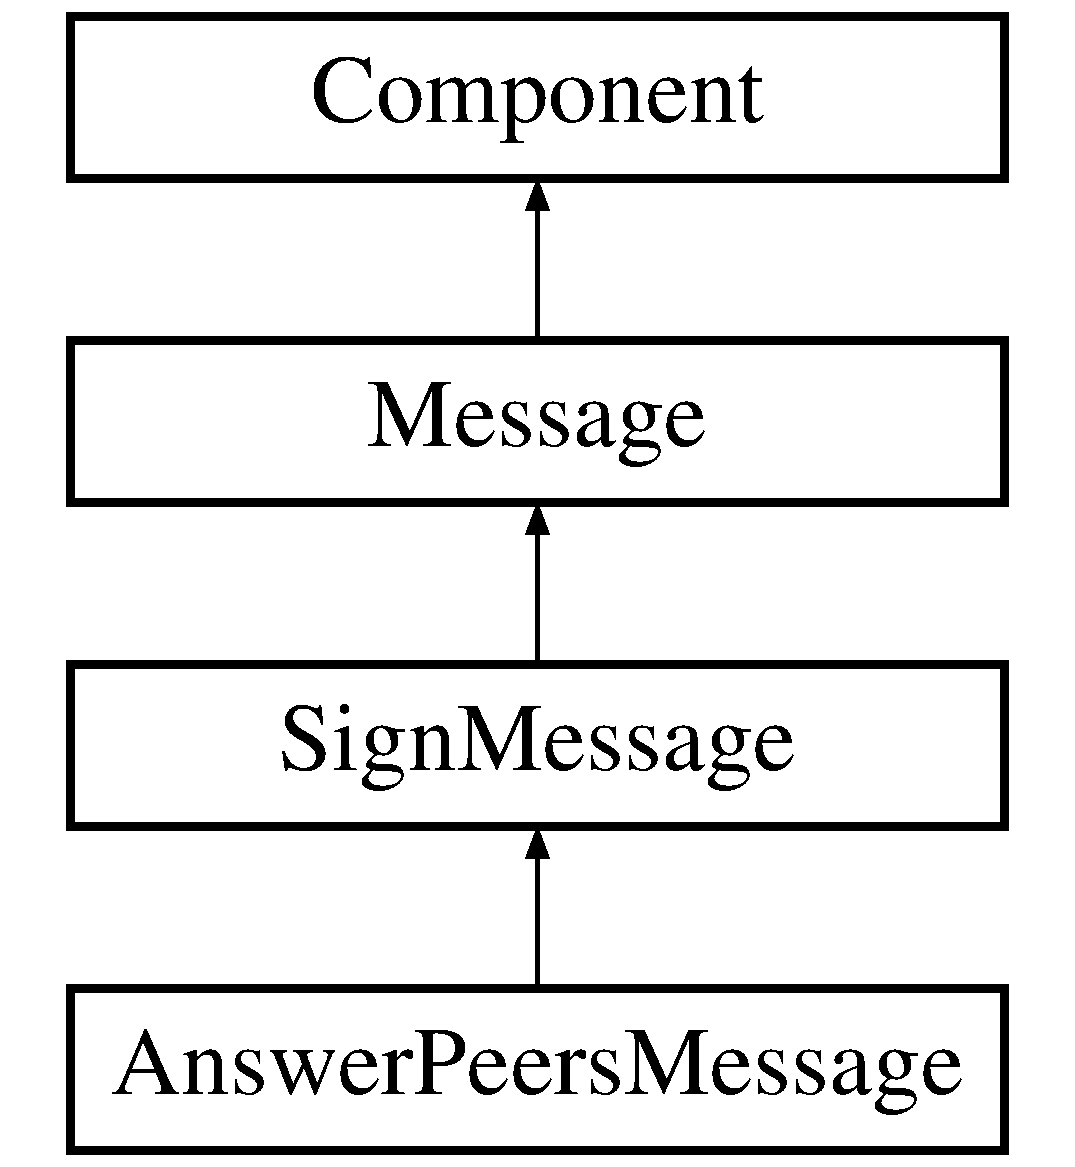
\includegraphics[height=4.000000cm]{classAnswerPeersMessage}
\end{center}
\end{figure}
\subsection*{Public Member Functions}
\begin{DoxyCompactItemize}
\item 
\mbox{\hyperlink{classAnswerPeersMessage_a9e187dfc2df64053694b5151db765eee}{Answer\+Peers\+Message}} (std\+::string p)
\item 
\mbox{\hyperlink{classElement}{Element}} $\ast$ \mbox{\hyperlink{classSignMessage_aee897c4bf78df966b8cca95e589566e4}{to\+Element}} () const override
\item 
const int \mbox{\hyperlink{classMessage_a2a576dcffd45c4574fcdf2897ec26086}{get\+\_\+type}} () const
\item 
void \mbox{\hyperlink{classComponent_a28212595f8ee85fe009bd233bc99b2fc}{\+\_\+\+\_\+init\+\_\+\+\_\+}} (\mbox{\hyperlink{classElementObject}{Element\+Object}} $\ast$element, const \mbox{\hyperlink{classSerializer}{Serializer}} $\ast$s, const char $\ast$encoding)
\end{DoxyCompactItemize}
\subsection*{Static Public Member Functions}
\begin{DoxyCompactItemize}
\item 
static \mbox{\hyperlink{classMessage}{Message}} $\ast$ \mbox{\hyperlink{classMessage_ad92a0e1cfa5b5a503ec9c61833e3e5ea}{generate}} (int id)
\end{DoxyCompactItemize}
\subsection*{Static Public Attributes}
\begin{DoxyCompactItemize}
\item 
\mbox{\Hypertarget{classMessage_a18a7a0d3879210c798f3d84c820f03c1}\label{classMessage_a18a7a0d3879210c798f3d84c820f03c1}} 
static const int {\bfseries T\+R\+A\+N\+S\+A\+C\+T\+I\+ON} = 4
\item 
\mbox{\Hypertarget{classMessage_a3d3ef3111518cd65c0b7f5ec6660888a}\label{classMessage_a3d3ef3111518cd65c0b7f5ec6660888a}} 
static const int {\bfseries B\+L\+O\+CK} = 5
\item 
\mbox{\Hypertarget{classMessage_a9810d3cefb1b33e709cb393583a7a877}\label{classMessage_a9810d3cefb1b33e709cb393583a7a877}} 
static const int {\bfseries A\+S\+K\+\_\+\+P\+E\+E\+RS} = 0
\item 
\mbox{\Hypertarget{classMessage_aa33f42e5795c4df01c7437961d512eaa}\label{classMessage_aa33f42e5795c4df01c7437961d512eaa}} 
static const int {\bfseries A\+N\+S\+W\+E\+R\+\_\+\+P\+E\+E\+RS} = 1
\item 
\mbox{\Hypertarget{classMessage_a64b7688dfdd50a6254bf45b51d2118d4}\label{classMessage_a64b7688dfdd50a6254bf45b51d2118d4}} 
static const int {\bfseries S\+I\+G\+N\+\_\+\+IN} = 2
\item 
\mbox{\Hypertarget{classMessage_aba70c352293fee66004d729ccef3ee48}\label{classMessage_aba70c352293fee66004d729ccef3ee48}} 
static const int {\bfseries S\+I\+G\+N\+\_\+\+O\+UT} = 3
\item 
\mbox{\Hypertarget{classMessage_a62ac5b91838e79a11079869015261e14}\label{classMessage_a62ac5b91838e79a11079869015261e14}} 
static const int {\bfseries A\+S\+K\+\_\+\+B\+L\+O\+CK} = 6
\item 
\mbox{\Hypertarget{classMessage_a1580f4a26d125f71e2af1ef6001ac656}\label{classMessage_a1580f4a26d125f71e2af1ef6001ac656}} 
static const int {\bfseries A\+N\+S\+W\+E\+R\+\_\+\+B\+L\+O\+CK} = 7
\end{DoxyCompactItemize}
\subsection*{Protected Member Functions}
\begin{DoxyCompactItemize}
\item 
void \mbox{\hyperlink{classSignMessage_a35855647925ec76036ed4602743ed118}{from\+Element}} (\mbox{\hyperlink{classElementObject}{Element\+Object}} $\ast$, const \mbox{\hyperlink{classSerializer}{Serializer}} $\ast$serializer, const char $\ast$encoding) override
\end{DoxyCompactItemize}
\subsection*{Protected Attributes}
\begin{DoxyCompactItemize}
\item 
int \mbox{\hyperlink{classMessage_afbfb481c98b13d0deba0bac443bebe29}{type}}
\end{DoxyCompactItemize}


\subsection{Detailed Description}
An answer peers message for sending the peers list \begin{DoxySeeAlso}{See also}
\mbox{\hyperlink{classSignMessage}{Sign\+Message}}
\end{DoxySeeAlso}
\begin{DoxyAuthor}{Author}
Mathieu Lochet 
\end{DoxyAuthor}
\begin{DoxyVersion}{Version}
1 
\end{DoxyVersion}


\subsection{Constructor \& Destructor Documentation}
\mbox{\Hypertarget{classAnswerPeersMessage_a9e187dfc2df64053694b5151db765eee}\label{classAnswerPeersMessage_a9e187dfc2df64053694b5151db765eee}} 
\index{Answer\+Peers\+Message@{Answer\+Peers\+Message}!Answer\+Peers\+Message@{Answer\+Peers\+Message}}
\index{Answer\+Peers\+Message@{Answer\+Peers\+Message}!Answer\+Peers\+Message@{Answer\+Peers\+Message}}
\subsubsection{\texorpdfstring{Answer\+Peers\+Message()}{AnswerPeersMessage()}}
{\footnotesize\ttfamily Answer\+Peers\+Message\+::\+Answer\+Peers\+Message (\begin{DoxyParamCaption}\item[{std\+::string}]{p }\end{DoxyParamCaption})}

Creates a answer peers message with a text Calls the super constructor with the type value \begin{DoxySeeAlso}{See also}
Message\+::\+A\+N\+S\+W\+E\+R\+\_\+\+P\+E\+E\+RS
\end{DoxySeeAlso}

\begin{DoxyParams}{Parameters}
{\em p} & The list of peers as a string value \\
\hline
\end{DoxyParams}


\subsection{Member Function Documentation}
\mbox{\Hypertarget{classComponent_a28212595f8ee85fe009bd233bc99b2fc}\label{classComponent_a28212595f8ee85fe009bd233bc99b2fc}} 
\index{Answer\+Peers\+Message@{Answer\+Peers\+Message}!\+\_\+\+\_\+init\+\_\+\+\_\+@{\+\_\+\+\_\+init\+\_\+\+\_\+}}
\index{\+\_\+\+\_\+init\+\_\+\+\_\+@{\+\_\+\+\_\+init\+\_\+\+\_\+}!Answer\+Peers\+Message@{Answer\+Peers\+Message}}
\subsubsection{\texorpdfstring{\+\_\+\+\_\+init\+\_\+\+\_\+()}{\_\_init\_\_()}}
{\footnotesize\ttfamily void Component\+::\+\_\+\+\_\+init\+\_\+\+\_\+ (\begin{DoxyParamCaption}\item[{\mbox{\hyperlink{classElementObject}{Element\+Object}} $\ast$}]{element,  }\item[{const \mbox{\hyperlink{classSerializer}{Serializer}} $\ast$}]{s,  }\item[{const char $\ast$}]{encoding }\end{DoxyParamCaption})\hspace{0.3cm}{\ttfamily [inline]}, {\ttfamily [inherited]}}

The function called by the serializer to initialize the object if it is empty \begin{DoxySeeAlso}{See also}
\mbox{\hyperlink{classElementObject}{Element\+Object}} 

\mbox{\hyperlink{classSerializer}{Serializer}}
\end{DoxySeeAlso}

\begin{DoxyParams}{Parameters}
{\em element} & The \mbox{\hyperlink{classElement}{Element}} representation of the object \\
\hline
{\em s} & The serializer (Can be used if serialization of some elements is needed) \\
\hline
{\em encoding} & The encoding that has been used to create the \mbox{\hyperlink{classElement}{Element}} representation of the object (Can be used if serialization of some elements is needed) \\
\hline
\end{DoxyParams}
\mbox{\Hypertarget{classSignMessage_a35855647925ec76036ed4602743ed118}\label{classSignMessage_a35855647925ec76036ed4602743ed118}} 
\index{Answer\+Peers\+Message@{Answer\+Peers\+Message}!from\+Element@{from\+Element}}
\index{from\+Element@{from\+Element}!Answer\+Peers\+Message@{Answer\+Peers\+Message}}
\subsubsection{\texorpdfstring{from\+Element()}{fromElement()}}
{\footnotesize\ttfamily void Sign\+Message\+::from\+Element (\begin{DoxyParamCaption}\item[{\mbox{\hyperlink{classElementObject}{Element\+Object}} $\ast$}]{,  }\item[{const \mbox{\hyperlink{classSerializer}{Serializer}} $\ast$}]{,  }\item[{const char $\ast$}]{encoding }\end{DoxyParamCaption})\hspace{0.3cm}{\ttfamily [override]}, {\ttfamily [protected]}, {\ttfamily [virtual]}, {\ttfamily [inherited]}}

The function used to build the object from its element representation. the object if it is empty \begin{DoxySeeAlso}{See also}
\mbox{\hyperlink{classElementObject}{Element\+Object}} 

\mbox{\hyperlink{classSerializer}{Serializer}}
\end{DoxySeeAlso}

\begin{DoxyParams}{Parameters}
{\em element} & The \mbox{\hyperlink{classElement}{Element}} representation of the object \\
\hline
{\em s} & The serializer (Can be used if serialization of some elements is needed) \\
\hline
{\em encoding} & The encoding that has been used to create the \mbox{\hyperlink{classElement}{Element}} representation of the object (Can be used if serialization of some elements is needed) \\
\hline
\end{DoxyParams}


Implements \mbox{\hyperlink{classComponent_a2ded18881226d0077dc393e0e9304bb1}{Component}}.

\mbox{\Hypertarget{classMessage_ad92a0e1cfa5b5a503ec9c61833e3e5ea}\label{classMessage_ad92a0e1cfa5b5a503ec9c61833e3e5ea}} 
\index{Answer\+Peers\+Message@{Answer\+Peers\+Message}!generate@{generate}}
\index{generate@{generate}!Answer\+Peers\+Message@{Answer\+Peers\+Message}}
\subsubsection{\texorpdfstring{generate()}{generate()}}
{\footnotesize\ttfamily \mbox{\hyperlink{classMessage}{Message}} $\ast$ Message\+::generate (\begin{DoxyParamCaption}\item[{int}]{id }\end{DoxyParamCaption})\hspace{0.3cm}{\ttfamily [static]}, {\ttfamily [inherited]}}

The message factory\+: creates the corresponding type of message with a given type. The generated message is empty and needs to be fill. \begin{DoxySeeAlso}{See also}
\mbox{\hyperlink{classComponent}{Component}}\+:\+:{\bfseries init}
\end{DoxySeeAlso}

\begin{DoxyParams}{Parameters}
{\em id} & the given type of the wanted message \\
\hline
\end{DoxyParams}
\begin{DoxyReturn}{Returns}
The type of the message 
\end{DoxyReturn}
\mbox{\Hypertarget{classMessage_a2a576dcffd45c4574fcdf2897ec26086}\label{classMessage_a2a576dcffd45c4574fcdf2897ec26086}} 
\index{Answer\+Peers\+Message@{Answer\+Peers\+Message}!get\+\_\+type@{get\+\_\+type}}
\index{get\+\_\+type@{get\+\_\+type}!Answer\+Peers\+Message@{Answer\+Peers\+Message}}
\subsubsection{\texorpdfstring{get\+\_\+type()}{get\_type()}}
{\footnotesize\ttfamily const int Message\+::get\+\_\+type (\begin{DoxyParamCaption}{ }\end{DoxyParamCaption}) const\hspace{0.3cm}{\ttfamily [inherited]}}

Get the type of the message

\begin{DoxyReturn}{Returns}
The type of the message 
\end{DoxyReturn}
\mbox{\Hypertarget{classSignMessage_aee897c4bf78df966b8cca95e589566e4}\label{classSignMessage_aee897c4bf78df966b8cca95e589566e4}} 
\index{Answer\+Peers\+Message@{Answer\+Peers\+Message}!to\+Element@{to\+Element}}
\index{to\+Element@{to\+Element}!Answer\+Peers\+Message@{Answer\+Peers\+Message}}
\subsubsection{\texorpdfstring{to\+Element()}{toElement()}}
{\footnotesize\ttfamily \mbox{\hyperlink{classElement}{Element}} $\ast$ Sign\+Message\+::to\+Element (\begin{DoxyParamCaption}{ }\end{DoxyParamCaption}) const\hspace{0.3cm}{\ttfamily [override]}, {\ttfamily [virtual]}, {\ttfamily [inherited]}}

The method used by the serializer to transform an object into an \mbox{\hyperlink{classElement}{Element}} representation. \begin{DoxySeeAlso}{See also}
\mbox{\hyperlink{classElement}{Element}}
\end{DoxySeeAlso}
\begin{DoxyReturn}{Returns}
The \mbox{\hyperlink{classElement}{Element}} representation of the object 
\end{DoxyReturn}


Implements \mbox{\hyperlink{classComponent_a3e63d8c993e417a4af3f56d65ebfc7ea}{Component}}.



\subsection{Member Data Documentation}
\mbox{\Hypertarget{classMessage_afbfb481c98b13d0deba0bac443bebe29}\label{classMessage_afbfb481c98b13d0deba0bac443bebe29}} 
\index{Answer\+Peers\+Message@{Answer\+Peers\+Message}!type@{type}}
\index{type@{type}!Answer\+Peers\+Message@{Answer\+Peers\+Message}}
\subsubsection{\texorpdfstring{type}{type}}
{\footnotesize\ttfamily int Message\+::type\hspace{0.3cm}{\ttfamily [protected]}, {\ttfamily [inherited]}}

The type of the message 

The documentation for this class was generated from the following files\+:\begin{DoxyCompactItemize}
\item 
block\+\_\+chain/kernel/messages/Answer\+Peers\+Message.\+h\item 
block\+\_\+chain/kernel/messages/Answer\+Peers\+Message.\+cpp\end{DoxyCompactItemize}

\hypertarget{classAskPeersMessage}{}\section{Ask\+Peers\+Message Class Reference}
\label{classAskPeersMessage}\index{Ask\+Peers\+Message@{Ask\+Peers\+Message}}


{\ttfamily \#include $<$Ask\+Peers\+Message.\+h$>$}

Inheritance diagram for Ask\+Peers\+Message\+:\begin{figure}[H]
\begin{center}
\leavevmode
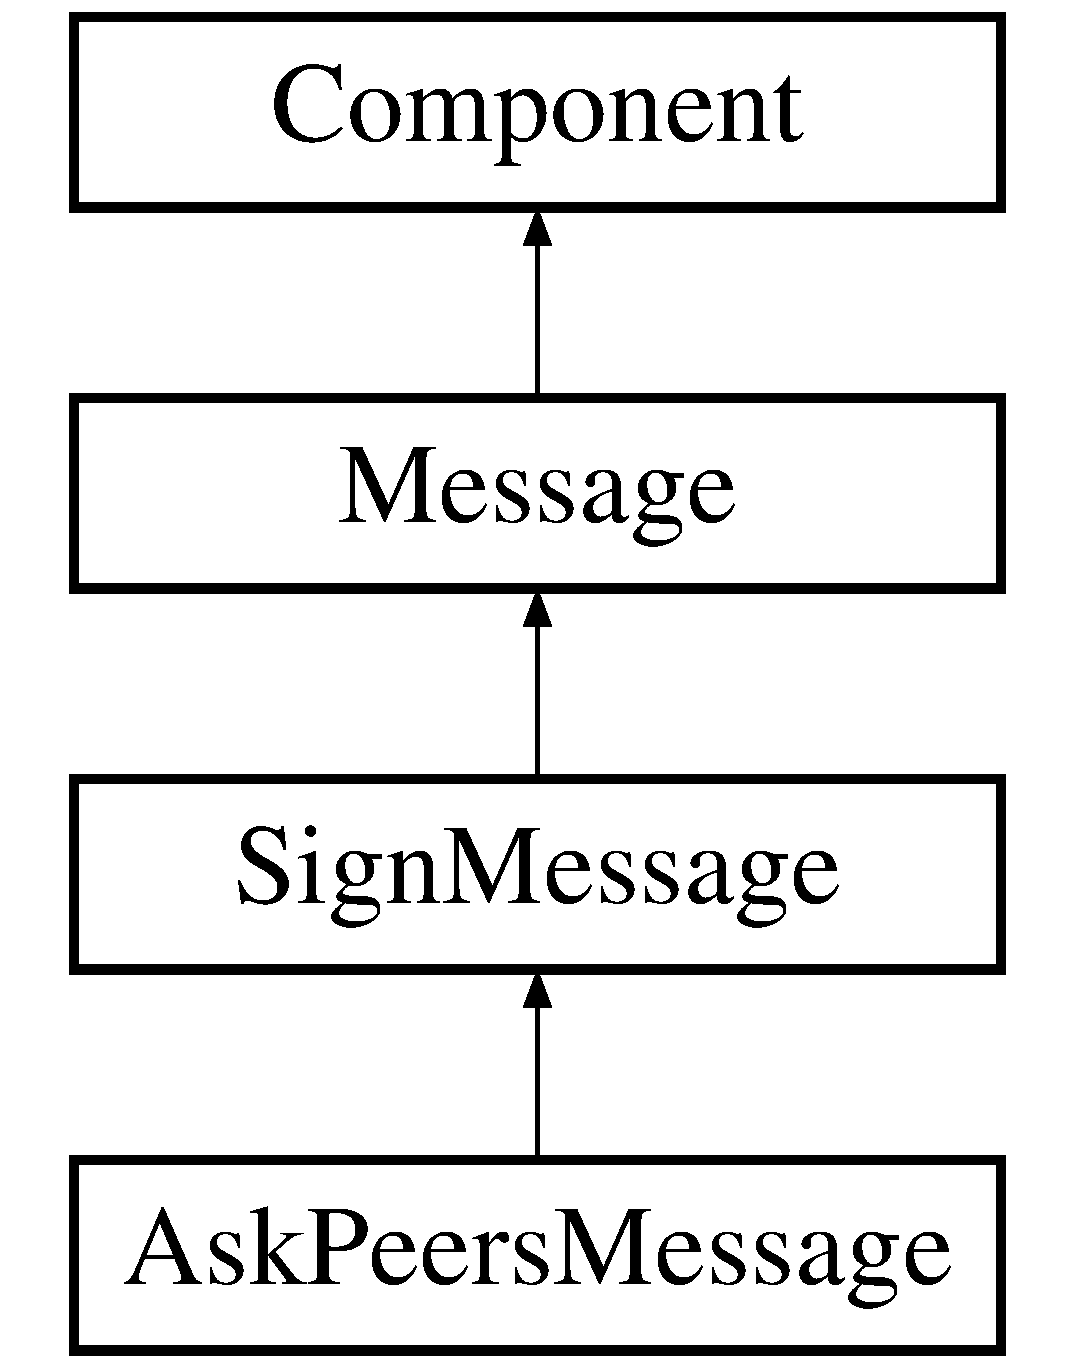
\includegraphics[height=4.000000cm]{classAskPeersMessage}
\end{center}
\end{figure}
\subsection*{Public Member Functions}
\begin{DoxyCompactItemize}
\item 
\mbox{\hyperlink{classAskPeersMessage_a55a68df97385093ce959c101b2331bf5}{Ask\+Peers\+Message}} (std\+::string p)
\item 
\mbox{\hyperlink{classElement}{Element}} $\ast$ \mbox{\hyperlink{classSignMessage_aee897c4bf78df966b8cca95e589566e4}{to\+Element}} () const override
\item 
const int \mbox{\hyperlink{classMessage_a2a576dcffd45c4574fcdf2897ec26086}{get\+\_\+type}} () const
\item 
void \mbox{\hyperlink{classComponent_a28212595f8ee85fe009bd233bc99b2fc}{\+\_\+\+\_\+init\+\_\+\+\_\+}} (\mbox{\hyperlink{classElementObject}{Element\+Object}} $\ast$element, const \mbox{\hyperlink{classSerializer}{Serializer}} $\ast$s, const char $\ast$encoding)
\end{DoxyCompactItemize}
\subsection*{Static Public Member Functions}
\begin{DoxyCompactItemize}
\item 
static \mbox{\hyperlink{classMessage}{Message}} $\ast$ \mbox{\hyperlink{classMessage_ad92a0e1cfa5b5a503ec9c61833e3e5ea}{generate}} (int id)
\end{DoxyCompactItemize}
\subsection*{Static Public Attributes}
\begin{DoxyCompactItemize}
\item 
\mbox{\Hypertarget{classMessage_a18a7a0d3879210c798f3d84c820f03c1}\label{classMessage_a18a7a0d3879210c798f3d84c820f03c1}} 
static const int {\bfseries T\+R\+A\+N\+S\+A\+C\+T\+I\+ON} = 4
\item 
\mbox{\Hypertarget{classMessage_a3d3ef3111518cd65c0b7f5ec6660888a}\label{classMessage_a3d3ef3111518cd65c0b7f5ec6660888a}} 
static const int {\bfseries B\+L\+O\+CK} = 5
\item 
\mbox{\Hypertarget{classMessage_a9810d3cefb1b33e709cb393583a7a877}\label{classMessage_a9810d3cefb1b33e709cb393583a7a877}} 
static const int {\bfseries A\+S\+K\+\_\+\+P\+E\+E\+RS} = 0
\item 
\mbox{\Hypertarget{classMessage_aa33f42e5795c4df01c7437961d512eaa}\label{classMessage_aa33f42e5795c4df01c7437961d512eaa}} 
static const int {\bfseries A\+N\+S\+W\+E\+R\+\_\+\+P\+E\+E\+RS} = 1
\item 
\mbox{\Hypertarget{classMessage_a64b7688dfdd50a6254bf45b51d2118d4}\label{classMessage_a64b7688dfdd50a6254bf45b51d2118d4}} 
static const int {\bfseries S\+I\+G\+N\+\_\+\+IN} = 2
\item 
\mbox{\Hypertarget{classMessage_aba70c352293fee66004d729ccef3ee48}\label{classMessage_aba70c352293fee66004d729ccef3ee48}} 
static const int {\bfseries S\+I\+G\+N\+\_\+\+O\+UT} = 3
\item 
\mbox{\Hypertarget{classMessage_a62ac5b91838e79a11079869015261e14}\label{classMessage_a62ac5b91838e79a11079869015261e14}} 
static const int {\bfseries A\+S\+K\+\_\+\+B\+L\+O\+CK} = 6
\item 
\mbox{\Hypertarget{classMessage_a1580f4a26d125f71e2af1ef6001ac656}\label{classMessage_a1580f4a26d125f71e2af1ef6001ac656}} 
static const int {\bfseries A\+N\+S\+W\+E\+R\+\_\+\+B\+L\+O\+CK} = 7
\end{DoxyCompactItemize}
\subsection*{Protected Member Functions}
\begin{DoxyCompactItemize}
\item 
void \mbox{\hyperlink{classSignMessage_a35855647925ec76036ed4602743ed118}{from\+Element}} (\mbox{\hyperlink{classElementObject}{Element\+Object}} $\ast$, const \mbox{\hyperlink{classSerializer}{Serializer}} $\ast$serializer, const char $\ast$encoding) override
\end{DoxyCompactItemize}
\subsection*{Protected Attributes}
\begin{DoxyCompactItemize}
\item 
int \mbox{\hyperlink{classMessage_afbfb481c98b13d0deba0bac443bebe29}{type}}
\end{DoxyCompactItemize}


\subsection{Detailed Description}
An ask peers message for asking the peers list \begin{DoxySeeAlso}{See also}
\mbox{\hyperlink{classSignMessage}{Sign\+Message}}
\end{DoxySeeAlso}
\begin{DoxyAuthor}{Author}
Mathieu Lochet 
\end{DoxyAuthor}
\begin{DoxyVersion}{Version}
1 
\end{DoxyVersion}


\subsection{Constructor \& Destructor Documentation}
\mbox{\Hypertarget{classAskPeersMessage_a55a68df97385093ce959c101b2331bf5}\label{classAskPeersMessage_a55a68df97385093ce959c101b2331bf5}} 
\index{Ask\+Peers\+Message@{Ask\+Peers\+Message}!Ask\+Peers\+Message@{Ask\+Peers\+Message}}
\index{Ask\+Peers\+Message@{Ask\+Peers\+Message}!Ask\+Peers\+Message@{Ask\+Peers\+Message}}
\subsubsection{\texorpdfstring{Ask\+Peers\+Message()}{AskPeersMessage()}}
{\footnotesize\ttfamily Ask\+Peers\+Message\+::\+Ask\+Peers\+Message (\begin{DoxyParamCaption}\item[{std\+::string}]{p }\end{DoxyParamCaption})}

Creates a ask peers message with a text Calls the super constructor with the type value \begin{DoxySeeAlso}{See also}
Message\+::\+A\+S\+K\+\_\+\+P\+E\+E\+RS
\end{DoxySeeAlso}

\begin{DoxyParams}{Parameters}
{\em p} & The users\textquotesingle{}s peer representation \\
\hline
\end{DoxyParams}


\subsection{Member Function Documentation}
\mbox{\Hypertarget{classComponent_a28212595f8ee85fe009bd233bc99b2fc}\label{classComponent_a28212595f8ee85fe009bd233bc99b2fc}} 
\index{Ask\+Peers\+Message@{Ask\+Peers\+Message}!\+\_\+\+\_\+init\+\_\+\+\_\+@{\+\_\+\+\_\+init\+\_\+\+\_\+}}
\index{\+\_\+\+\_\+init\+\_\+\+\_\+@{\+\_\+\+\_\+init\+\_\+\+\_\+}!Ask\+Peers\+Message@{Ask\+Peers\+Message}}
\subsubsection{\texorpdfstring{\+\_\+\+\_\+init\+\_\+\+\_\+()}{\_\_init\_\_()}}
{\footnotesize\ttfamily void Component\+::\+\_\+\+\_\+init\+\_\+\+\_\+ (\begin{DoxyParamCaption}\item[{\mbox{\hyperlink{classElementObject}{Element\+Object}} $\ast$}]{element,  }\item[{const \mbox{\hyperlink{classSerializer}{Serializer}} $\ast$}]{s,  }\item[{const char $\ast$}]{encoding }\end{DoxyParamCaption})\hspace{0.3cm}{\ttfamily [inline]}, {\ttfamily [inherited]}}

The function called by the serializer to initialize the object if it is empty \begin{DoxySeeAlso}{See also}
\mbox{\hyperlink{classElementObject}{Element\+Object}} 

\mbox{\hyperlink{classSerializer}{Serializer}}
\end{DoxySeeAlso}

\begin{DoxyParams}{Parameters}
{\em element} & The \mbox{\hyperlink{classElement}{Element}} representation of the object \\
\hline
{\em s} & The serializer (Can be used if serialization of some elements is needed) \\
\hline
{\em encoding} & The encoding that has been used to create the \mbox{\hyperlink{classElement}{Element}} representation of the object (Can be used if serialization of some elements is needed) \\
\hline
\end{DoxyParams}
\mbox{\Hypertarget{classSignMessage_a35855647925ec76036ed4602743ed118}\label{classSignMessage_a35855647925ec76036ed4602743ed118}} 
\index{Ask\+Peers\+Message@{Ask\+Peers\+Message}!from\+Element@{from\+Element}}
\index{from\+Element@{from\+Element}!Ask\+Peers\+Message@{Ask\+Peers\+Message}}
\subsubsection{\texorpdfstring{from\+Element()}{fromElement()}}
{\footnotesize\ttfamily void Sign\+Message\+::from\+Element (\begin{DoxyParamCaption}\item[{\mbox{\hyperlink{classElementObject}{Element\+Object}} $\ast$}]{,  }\item[{const \mbox{\hyperlink{classSerializer}{Serializer}} $\ast$}]{,  }\item[{const char $\ast$}]{encoding }\end{DoxyParamCaption})\hspace{0.3cm}{\ttfamily [override]}, {\ttfamily [protected]}, {\ttfamily [virtual]}, {\ttfamily [inherited]}}

The function used to build the object from its element representation. the object if it is empty \begin{DoxySeeAlso}{See also}
\mbox{\hyperlink{classElementObject}{Element\+Object}} 

\mbox{\hyperlink{classSerializer}{Serializer}}
\end{DoxySeeAlso}

\begin{DoxyParams}{Parameters}
{\em element} & The \mbox{\hyperlink{classElement}{Element}} representation of the object \\
\hline
{\em s} & The serializer (Can be used if serialization of some elements is needed) \\
\hline
{\em encoding} & The encoding that has been used to create the \mbox{\hyperlink{classElement}{Element}} representation of the object (Can be used if serialization of some elements is needed) \\
\hline
\end{DoxyParams}


Implements \mbox{\hyperlink{classComponent_a2ded18881226d0077dc393e0e9304bb1}{Component}}.

\mbox{\Hypertarget{classMessage_ad92a0e1cfa5b5a503ec9c61833e3e5ea}\label{classMessage_ad92a0e1cfa5b5a503ec9c61833e3e5ea}} 
\index{Ask\+Peers\+Message@{Ask\+Peers\+Message}!generate@{generate}}
\index{generate@{generate}!Ask\+Peers\+Message@{Ask\+Peers\+Message}}
\subsubsection{\texorpdfstring{generate()}{generate()}}
{\footnotesize\ttfamily \mbox{\hyperlink{classMessage}{Message}} $\ast$ Message\+::generate (\begin{DoxyParamCaption}\item[{int}]{id }\end{DoxyParamCaption})\hspace{0.3cm}{\ttfamily [static]}, {\ttfamily [inherited]}}

The message factory\+: creates the corresponding type of message with a given type. The generated message is empty and needs to be fill. \begin{DoxySeeAlso}{See also}
\mbox{\hyperlink{classComponent}{Component}}\+:\+:{\bfseries init}
\end{DoxySeeAlso}

\begin{DoxyParams}{Parameters}
{\em id} & the given type of the wanted message \\
\hline
\end{DoxyParams}
\begin{DoxyReturn}{Returns}
The type of the message 
\end{DoxyReturn}
\mbox{\Hypertarget{classMessage_a2a576dcffd45c4574fcdf2897ec26086}\label{classMessage_a2a576dcffd45c4574fcdf2897ec26086}} 
\index{Ask\+Peers\+Message@{Ask\+Peers\+Message}!get\+\_\+type@{get\+\_\+type}}
\index{get\+\_\+type@{get\+\_\+type}!Ask\+Peers\+Message@{Ask\+Peers\+Message}}
\subsubsection{\texorpdfstring{get\+\_\+type()}{get\_type()}}
{\footnotesize\ttfamily const int Message\+::get\+\_\+type (\begin{DoxyParamCaption}{ }\end{DoxyParamCaption}) const\hspace{0.3cm}{\ttfamily [inherited]}}

Get the type of the message

\begin{DoxyReturn}{Returns}
The type of the message 
\end{DoxyReturn}
\mbox{\Hypertarget{classSignMessage_aee897c4bf78df966b8cca95e589566e4}\label{classSignMessage_aee897c4bf78df966b8cca95e589566e4}} 
\index{Ask\+Peers\+Message@{Ask\+Peers\+Message}!to\+Element@{to\+Element}}
\index{to\+Element@{to\+Element}!Ask\+Peers\+Message@{Ask\+Peers\+Message}}
\subsubsection{\texorpdfstring{to\+Element()}{toElement()}}
{\footnotesize\ttfamily \mbox{\hyperlink{classElement}{Element}} $\ast$ Sign\+Message\+::to\+Element (\begin{DoxyParamCaption}{ }\end{DoxyParamCaption}) const\hspace{0.3cm}{\ttfamily [override]}, {\ttfamily [virtual]}, {\ttfamily [inherited]}}

The method used by the serializer to transform an object into an \mbox{\hyperlink{classElement}{Element}} representation. \begin{DoxySeeAlso}{See also}
\mbox{\hyperlink{classElement}{Element}}
\end{DoxySeeAlso}
\begin{DoxyReturn}{Returns}
The \mbox{\hyperlink{classElement}{Element}} representation of the object 
\end{DoxyReturn}


Implements \mbox{\hyperlink{classComponent_a3e63d8c993e417a4af3f56d65ebfc7ea}{Component}}.



\subsection{Member Data Documentation}
\mbox{\Hypertarget{classMessage_afbfb481c98b13d0deba0bac443bebe29}\label{classMessage_afbfb481c98b13d0deba0bac443bebe29}} 
\index{Ask\+Peers\+Message@{Ask\+Peers\+Message}!type@{type}}
\index{type@{type}!Ask\+Peers\+Message@{Ask\+Peers\+Message}}
\subsubsection{\texorpdfstring{type}{type}}
{\footnotesize\ttfamily int Message\+::type\hspace{0.3cm}{\ttfamily [protected]}, {\ttfamily [inherited]}}

The type of the message 

The documentation for this class was generated from the following files\+:\begin{DoxyCompactItemize}
\item 
block\+\_\+chain/kernel/messages/Ask\+Peers\+Message.\+h\item 
block\+\_\+chain/kernel/messages/Ask\+Peers\+Message.\+cpp\end{DoxyCompactItemize}

\hypertarget{classBlock}{}\section{Block Class Reference}
\label{classBlock}\index{Block@{Block}}
Inheritance diagram for Block\+:\begin{figure}[H]
\begin{center}
\leavevmode
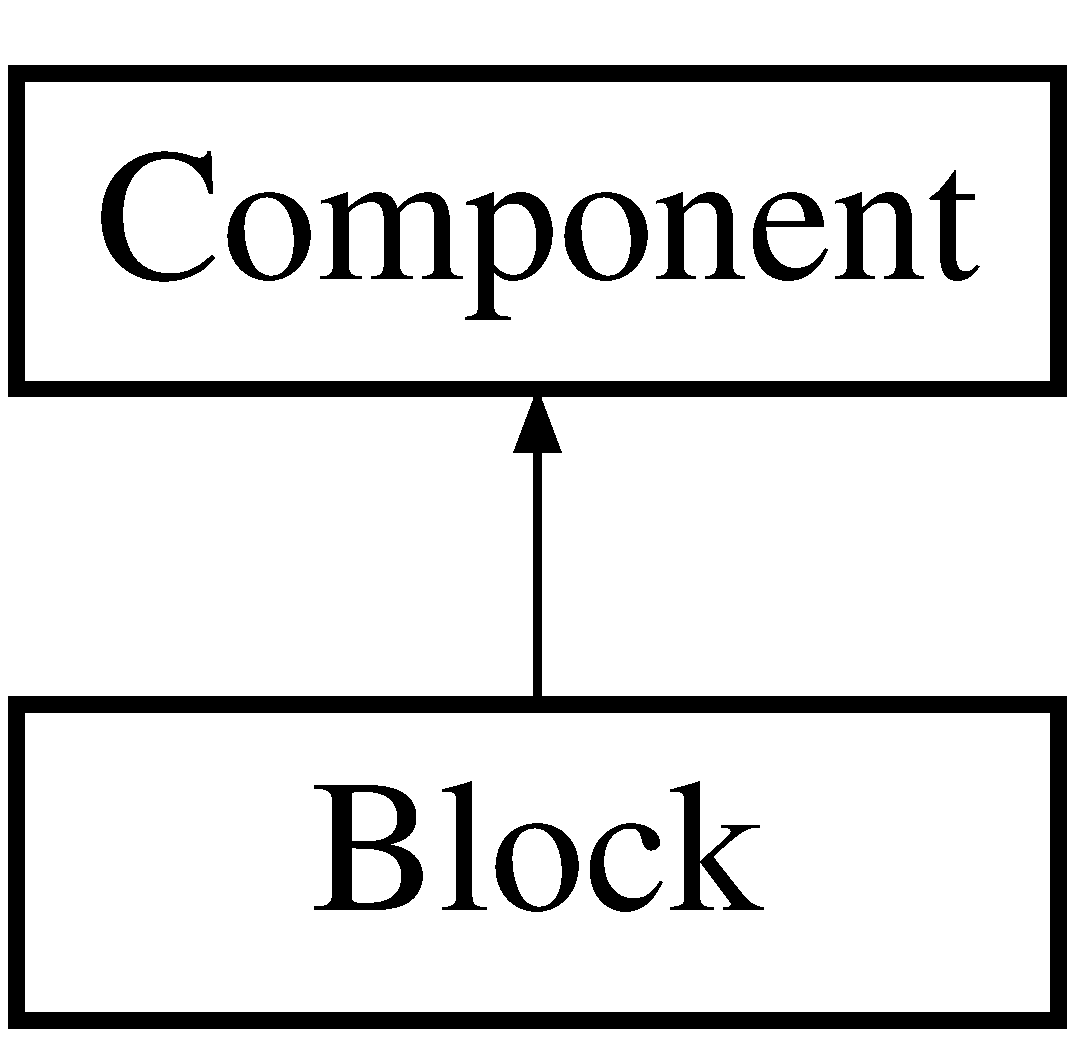
\includegraphics[height=2.000000cm]{classBlock}
\end{center}
\end{figure}
\subsection*{Public Member Functions}
\begin{DoxyCompactItemize}
\item 
\mbox{\Hypertarget{classBlock_a02178e246d2e99fcdc58f8401776387a}\label{classBlock_a02178e246d2e99fcdc58f8401776387a}} 
{\bfseries Block} (const \mbox{\hyperlink{classSerializer}{Serializer}} $\ast$, const char $\ast$)
\item 
\mbox{\Hypertarget{classBlock_a52b897f6b8fbaccc0d18aa5fe677af9f}\label{classBlock_a52b897f6b8fbaccc0d18aa5fe677af9f}} 
{\bfseries Block} (std\+::vector$<$ std\+::pair$<$ std\+::string, std\+::string $>$$>$ transactions, \mbox{\hyperlink{classHash}{Hash}} $\ast$, const \mbox{\hyperlink{classSerializer}{Serializer}} $\ast$s, const char $\ast$e)
\item 
\mbox{\Hypertarget{classBlock_aa289363a40f0d3ba88720ad0bc71f34f}\label{classBlock_aa289363a40f0d3ba88720ad0bc71f34f}} 
\mbox{\hyperlink{classElement}{Element}} $\ast$ {\bfseries to\+Element} () const override
\item 
\mbox{\Hypertarget{classBlock_a24fef11a9eaf9b23490a734be5e30f30}\label{classBlock_a24fef11a9eaf9b23490a734be5e30f30}} 
bool {\bfseries operator==} (\mbox{\hyperlink{classBlock}{Block}} $\ast$block) const
\item 
\mbox{\Hypertarget{classBlock_ab9d7e32509fb1ab4ca2bb63854f52cc3}\label{classBlock_ab9d7e32509fb1ab4ca2bb63854f52cc3}} 
\mbox{\hyperlink{classHash}{Hash}} $\ast$ {\bfseries compute\+\_\+fingerprint} (const \mbox{\hyperlink{classSerializer}{Serializer}} $\ast$s, const char $\ast$e) const
\item 
\mbox{\Hypertarget{classBlock_a0755737dbbca68ee6a1ca62340843746}\label{classBlock_a0755737dbbca68ee6a1ca62340843746}} 
bool {\bfseries check\+Finger\+Print} (const \mbox{\hyperlink{classSerializer}{Serializer}} $\ast$s, const char $\ast$e) const
\item 
\mbox{\Hypertarget{classBlock_a1c8ebc79bd2ad82d138ee8159899baf6}\label{classBlock_a1c8ebc79bd2ad82d138ee8159899baf6}} 
virtual std\+::string {\bfseries to\+\_\+string} () const
\item 
\mbox{\Hypertarget{classBlock_afb50015ba1d705fc5ef5e12bb1cd1a56}\label{classBlock_afb50015ba1d705fc5ef5e12bb1cd1a56}} 
void {\bfseries update\+\_\+fingerprint} ()
\item 
\mbox{\Hypertarget{classComponent_a28212595f8ee85fe009bd233bc99b2fc}\label{classComponent_a28212595f8ee85fe009bd233bc99b2fc}} 
void {\bfseries \+\_\+\+\_\+init\+\_\+\+\_\+} (\mbox{\hyperlink{classElementObject}{Element\+Object}} $\ast$element, const \mbox{\hyperlink{classSerializer}{Serializer}} $\ast$s, const char $\ast$encoding)
\end{DoxyCompactItemize}
\subsection*{Protected Member Functions}
\begin{DoxyCompactItemize}
\item 
\mbox{\Hypertarget{classBlock_ab21c6536cf7a26fdf2a2e889a84fcb9d}\label{classBlock_ab21c6536cf7a26fdf2a2e889a84fcb9d}} 
void {\bfseries from\+Element} (\mbox{\hyperlink{classElementObject}{Element\+Object}} $\ast$e, const \mbox{\hyperlink{classSerializer}{Serializer}} $\ast$s, const char $\ast$encoding) override
\end{DoxyCompactItemize}
\subsection*{Friends}
\begin{DoxyCompactItemize}
\item 
\mbox{\Hypertarget{classBlock_adfdd1242f00ef4da9a9a01d996fc292c}\label{classBlock_adfdd1242f00ef4da9a9a01d996fc292c}} 
class {\bfseries Node\+State}
\item 
\mbox{\Hypertarget{classBlock_a6db9d28bd448a131448276ee03de1e6d}\label{classBlock_a6db9d28bd448a131448276ee03de1e6d}} 
class {\bfseries Node}
\item 
\mbox{\Hypertarget{classBlock_a5493b64dfe8bc707452f326c6ec29f14}\label{classBlock_a5493b64dfe8bc707452f326c6ec29f14}} 
class {\bfseries Proof\+Of\+Work}
\item 
\mbox{\Hypertarget{classBlock_a65813570c30a3e0656fa523793ff1b86}\label{classBlock_a65813570c30a3e0656fa523793ff1b86}} 
class {\bfseries Chain}
\item 
\mbox{\Hypertarget{classBlock_a760b1478b5214c122458f0f19d45c127}\label{classBlock_a760b1478b5214c122458f0f19d45c127}} 
class {\bfseries Transaction\+Parser}
\item 
\mbox{\Hypertarget{classBlock_a8428b3aeea6607d1ba12e603ff9d015c}\label{classBlock_a8428b3aeea6607d1ba12e603ff9d015c}} 
class {\bfseries Block\+Parser}
\end{DoxyCompactItemize}


The documentation for this class was generated from the following files\+:\begin{DoxyCompactItemize}
\item 
block\+\_\+chain/chain/block/Block.\+h\item 
block\+\_\+chain/chain/block/Block.\+cpp\end{DoxyCompactItemize}

\hypertarget{classBlockAnswerMessage}{}\section{Block\+Answer\+Message Class Reference}
\label{classBlockAnswerMessage}\index{Block\+Answer\+Message@{Block\+Answer\+Message}}


{\ttfamily \#include $<$Block\+Answer\+Message.\+h$>$}

Inheritance diagram for Block\+Answer\+Message\+:\begin{figure}[H]
\begin{center}
\leavevmode
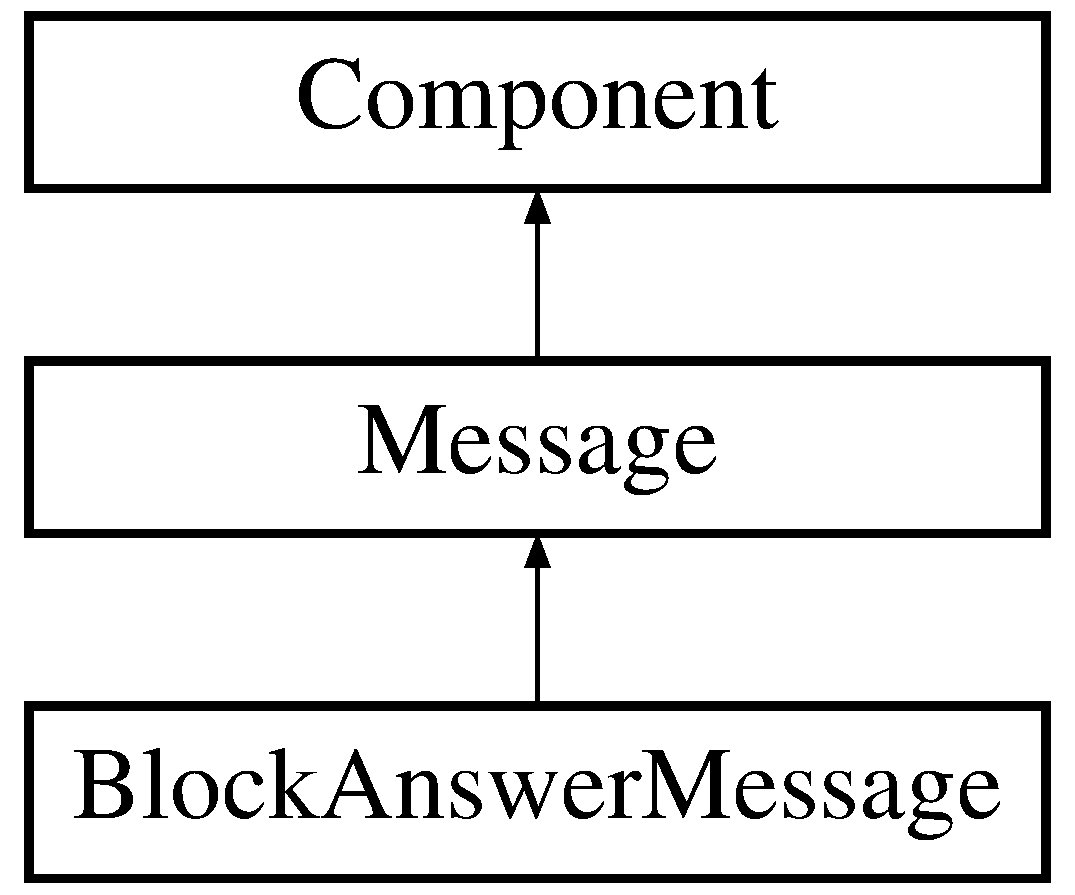
\includegraphics[height=3.000000cm]{classBlockAnswerMessage}
\end{center}
\end{figure}
\subsection*{Public Member Functions}
\begin{DoxyCompactItemize}
\item 
\mbox{\hyperlink{classBlockAnswerMessage_a7d562144e7ad2ff1c5ab8fdbc3d27d32}{Block\+Answer\+Message}} (std\+::string p)
\item 
\mbox{\hyperlink{classElement}{Element}} $\ast$ \mbox{\hyperlink{classBlockAnswerMessage_ac7f35ec9f7f2fbcd726628c2a984518b}{to\+Element}} () const override
\item 
const int \mbox{\hyperlink{classMessage_a2a576dcffd45c4574fcdf2897ec26086}{get\+\_\+type}} () const
\item 
void \mbox{\hyperlink{classComponent_a28212595f8ee85fe009bd233bc99b2fc}{\+\_\+\+\_\+init\+\_\+\+\_\+}} (\mbox{\hyperlink{classElementObject}{Element\+Object}} $\ast$element, const \mbox{\hyperlink{classSerializer}{Serializer}} $\ast$s, const char $\ast$encoding)
\end{DoxyCompactItemize}
\subsection*{Static Public Member Functions}
\begin{DoxyCompactItemize}
\item 
static \mbox{\hyperlink{classMessage}{Message}} $\ast$ \mbox{\hyperlink{classMessage_ad92a0e1cfa5b5a503ec9c61833e3e5ea}{generate}} (int id)
\end{DoxyCompactItemize}
\subsection*{Static Public Attributes}
\begin{DoxyCompactItemize}
\item 
\mbox{\Hypertarget{classMessage_a18a7a0d3879210c798f3d84c820f03c1}\label{classMessage_a18a7a0d3879210c798f3d84c820f03c1}} 
static const int {\bfseries T\+R\+A\+N\+S\+A\+C\+T\+I\+ON} = 4
\item 
\mbox{\Hypertarget{classMessage_a3d3ef3111518cd65c0b7f5ec6660888a}\label{classMessage_a3d3ef3111518cd65c0b7f5ec6660888a}} 
static const int {\bfseries B\+L\+O\+CK} = 5
\item 
\mbox{\Hypertarget{classMessage_a9810d3cefb1b33e709cb393583a7a877}\label{classMessage_a9810d3cefb1b33e709cb393583a7a877}} 
static const int {\bfseries A\+S\+K\+\_\+\+P\+E\+E\+RS} = 0
\item 
\mbox{\Hypertarget{classMessage_aa33f42e5795c4df01c7437961d512eaa}\label{classMessage_aa33f42e5795c4df01c7437961d512eaa}} 
static const int {\bfseries A\+N\+S\+W\+E\+R\+\_\+\+P\+E\+E\+RS} = 1
\item 
\mbox{\Hypertarget{classMessage_a64b7688dfdd50a6254bf45b51d2118d4}\label{classMessage_a64b7688dfdd50a6254bf45b51d2118d4}} 
static const int {\bfseries S\+I\+G\+N\+\_\+\+IN} = 2
\item 
\mbox{\Hypertarget{classMessage_aba70c352293fee66004d729ccef3ee48}\label{classMessage_aba70c352293fee66004d729ccef3ee48}} 
static const int {\bfseries S\+I\+G\+N\+\_\+\+O\+UT} = 3
\item 
\mbox{\Hypertarget{classMessage_a62ac5b91838e79a11079869015261e14}\label{classMessage_a62ac5b91838e79a11079869015261e14}} 
static const int {\bfseries A\+S\+K\+\_\+\+B\+L\+O\+CK} = 6
\item 
\mbox{\Hypertarget{classMessage_a1580f4a26d125f71e2af1ef6001ac656}\label{classMessage_a1580f4a26d125f71e2af1ef6001ac656}} 
static const int {\bfseries A\+N\+S\+W\+E\+R\+\_\+\+B\+L\+O\+CK} = 7
\end{DoxyCompactItemize}
\subsection*{Protected Member Functions}
\begin{DoxyCompactItemize}
\item 
void \mbox{\hyperlink{classBlockAnswerMessage_affa76e8a95365baf5c9eb409a0a19b9d}{from\+Element}} (\mbox{\hyperlink{classElementObject}{Element\+Object}} $\ast$, const \mbox{\hyperlink{classSerializer}{Serializer}} $\ast$serializer, const char $\ast$encoding) override
\end{DoxyCompactItemize}
\subsection*{Protected Attributes}
\begin{DoxyCompactItemize}
\item 
int \mbox{\hyperlink{classMessage_afbfb481c98b13d0deba0bac443bebe29}{type}}
\end{DoxyCompactItemize}
\subsection*{Friends}
\begin{DoxyCompactItemize}
\item 
\mbox{\Hypertarget{classBlockAnswerMessage_aec03b63df2dcea2b43f28ba4ede77b27}\label{classBlockAnswerMessage_aec03b63df2dcea2b43f28ba4ede77b27}} 
class {\bfseries Block\+Answer\+Parser}
\end{DoxyCompactItemize}


\subsection{Detailed Description}
An answer containing the required block \begin{DoxySeeAlso}{See also}
\mbox{\hyperlink{classMessage}{Message}}
\end{DoxySeeAlso}
\begin{DoxyAuthor}{Author}
Mathieu Lochet 
\end{DoxyAuthor}
\begin{DoxyVersion}{Version}
1 
\end{DoxyVersion}


\subsection{Constructor \& Destructor Documentation}
\mbox{\Hypertarget{classBlockAnswerMessage_a7d562144e7ad2ff1c5ab8fdbc3d27d32}\label{classBlockAnswerMessage_a7d562144e7ad2ff1c5ab8fdbc3d27d32}} 
\index{Block\+Answer\+Message@{Block\+Answer\+Message}!Block\+Answer\+Message@{Block\+Answer\+Message}}
\index{Block\+Answer\+Message@{Block\+Answer\+Message}!Block\+Answer\+Message@{Block\+Answer\+Message}}
\subsubsection{\texorpdfstring{Block\+Answer\+Message()}{BlockAnswerMessage()}}
{\footnotesize\ttfamily Block\+Answer\+Message\+::\+Block\+Answer\+Message (\begin{DoxyParamCaption}\item[{std\+::string}]{p }\end{DoxyParamCaption})}

Creates an answer to a block request Calls the super constructor with the type value \begin{DoxySeeAlso}{See also}
Message\+::\+A\+N\+S\+W\+E\+R\+\_\+\+B\+L\+O\+CK
\end{DoxySeeAlso}

\begin{DoxyParams}{Parameters}
{\em p} & The serialized block \\
\hline
\end{DoxyParams}


\subsection{Member Function Documentation}
\mbox{\Hypertarget{classComponent_a28212595f8ee85fe009bd233bc99b2fc}\label{classComponent_a28212595f8ee85fe009bd233bc99b2fc}} 
\index{Block\+Answer\+Message@{Block\+Answer\+Message}!\+\_\+\+\_\+init\+\_\+\+\_\+@{\+\_\+\+\_\+init\+\_\+\+\_\+}}
\index{\+\_\+\+\_\+init\+\_\+\+\_\+@{\+\_\+\+\_\+init\+\_\+\+\_\+}!Block\+Answer\+Message@{Block\+Answer\+Message}}
\subsubsection{\texorpdfstring{\+\_\+\+\_\+init\+\_\+\+\_\+()}{\_\_init\_\_()}}
{\footnotesize\ttfamily void Component\+::\+\_\+\+\_\+init\+\_\+\+\_\+ (\begin{DoxyParamCaption}\item[{\mbox{\hyperlink{classElementObject}{Element\+Object}} $\ast$}]{element,  }\item[{const \mbox{\hyperlink{classSerializer}{Serializer}} $\ast$}]{s,  }\item[{const char $\ast$}]{encoding }\end{DoxyParamCaption})\hspace{0.3cm}{\ttfamily [inline]}, {\ttfamily [inherited]}}

The function called by the serializer to initialize the object if it is empty \begin{DoxySeeAlso}{See also}
\mbox{\hyperlink{classElementObject}{Element\+Object}} 

\mbox{\hyperlink{classSerializer}{Serializer}}
\end{DoxySeeAlso}

\begin{DoxyParams}{Parameters}
{\em element} & The \mbox{\hyperlink{classElement}{Element}} representation of the object \\
\hline
{\em s} & The serializer (Can be used if serialization of some elements is needed) \\
\hline
{\em encoding} & The encoding that has been used to create the \mbox{\hyperlink{classElement}{Element}} representation of the object (Can be used if serialization of some elements is needed) \\
\hline
\end{DoxyParams}
\mbox{\Hypertarget{classBlockAnswerMessage_affa76e8a95365baf5c9eb409a0a19b9d}\label{classBlockAnswerMessage_affa76e8a95365baf5c9eb409a0a19b9d}} 
\index{Block\+Answer\+Message@{Block\+Answer\+Message}!from\+Element@{from\+Element}}
\index{from\+Element@{from\+Element}!Block\+Answer\+Message@{Block\+Answer\+Message}}
\subsubsection{\texorpdfstring{from\+Element()}{fromElement()}}
{\footnotesize\ttfamily void Block\+Answer\+Message\+::from\+Element (\begin{DoxyParamCaption}\item[{\mbox{\hyperlink{classElementObject}{Element\+Object}} $\ast$}]{,  }\item[{const \mbox{\hyperlink{classSerializer}{Serializer}} $\ast$}]{,  }\item[{const char $\ast$}]{encoding }\end{DoxyParamCaption})\hspace{0.3cm}{\ttfamily [override]}, {\ttfamily [protected]}, {\ttfamily [virtual]}}

The function used to build the object from its element representation. the object if it is empty \begin{DoxySeeAlso}{See also}
\mbox{\hyperlink{classElementObject}{Element\+Object}} 

\mbox{\hyperlink{classSerializer}{Serializer}}
\end{DoxySeeAlso}

\begin{DoxyParams}{Parameters}
{\em element} & The \mbox{\hyperlink{classElement}{Element}} representation of the object \\
\hline
{\em s} & The serializer (Can be used if serialization of some elements is needed) \\
\hline
{\em encoding} & The encoding that has been used to create the \mbox{\hyperlink{classElement}{Element}} representation of the object (Can be used if serialization of some elements is needed) \\
\hline
\end{DoxyParams}


Implements \mbox{\hyperlink{classComponent_a2ded18881226d0077dc393e0e9304bb1}{Component}}.

\mbox{\Hypertarget{classMessage_ad92a0e1cfa5b5a503ec9c61833e3e5ea}\label{classMessage_ad92a0e1cfa5b5a503ec9c61833e3e5ea}} 
\index{Block\+Answer\+Message@{Block\+Answer\+Message}!generate@{generate}}
\index{generate@{generate}!Block\+Answer\+Message@{Block\+Answer\+Message}}
\subsubsection{\texorpdfstring{generate()}{generate()}}
{\footnotesize\ttfamily \mbox{\hyperlink{classMessage}{Message}} $\ast$ Message\+::generate (\begin{DoxyParamCaption}\item[{int}]{id }\end{DoxyParamCaption})\hspace{0.3cm}{\ttfamily [static]}, {\ttfamily [inherited]}}

The message factory\+: creates the corresponding type of message with a given type. The generated message is empty and needs to be fill. \begin{DoxySeeAlso}{See also}
\mbox{\hyperlink{classComponent}{Component}}\+:\+:{\bfseries init}
\end{DoxySeeAlso}

\begin{DoxyParams}{Parameters}
{\em id} & the given type of the wanted message \\
\hline
\end{DoxyParams}
\begin{DoxyReturn}{Returns}
The type of the message 
\end{DoxyReturn}
\mbox{\Hypertarget{classMessage_a2a576dcffd45c4574fcdf2897ec26086}\label{classMessage_a2a576dcffd45c4574fcdf2897ec26086}} 
\index{Block\+Answer\+Message@{Block\+Answer\+Message}!get\+\_\+type@{get\+\_\+type}}
\index{get\+\_\+type@{get\+\_\+type}!Block\+Answer\+Message@{Block\+Answer\+Message}}
\subsubsection{\texorpdfstring{get\+\_\+type()}{get\_type()}}
{\footnotesize\ttfamily const int Message\+::get\+\_\+type (\begin{DoxyParamCaption}{ }\end{DoxyParamCaption}) const\hspace{0.3cm}{\ttfamily [inherited]}}

Get the type of the message

\begin{DoxyReturn}{Returns}
The type of the message 
\end{DoxyReturn}
\mbox{\Hypertarget{classBlockAnswerMessage_ac7f35ec9f7f2fbcd726628c2a984518b}\label{classBlockAnswerMessage_ac7f35ec9f7f2fbcd726628c2a984518b}} 
\index{Block\+Answer\+Message@{Block\+Answer\+Message}!to\+Element@{to\+Element}}
\index{to\+Element@{to\+Element}!Block\+Answer\+Message@{Block\+Answer\+Message}}
\subsubsection{\texorpdfstring{to\+Element()}{toElement()}}
{\footnotesize\ttfamily \mbox{\hyperlink{classElement}{Element}} $\ast$ Block\+Answer\+Message\+::to\+Element (\begin{DoxyParamCaption}{ }\end{DoxyParamCaption}) const\hspace{0.3cm}{\ttfamily [override]}, {\ttfamily [virtual]}}

The method used by the serializer to transform an object into an \mbox{\hyperlink{classElement}{Element}} representation. \begin{DoxySeeAlso}{See also}
\mbox{\hyperlink{classElement}{Element}}
\end{DoxySeeAlso}
\begin{DoxyReturn}{Returns}
The \mbox{\hyperlink{classElement}{Element}} representation of the object 
\end{DoxyReturn}


Implements \mbox{\hyperlink{classComponent_a3e63d8c993e417a4af3f56d65ebfc7ea}{Component}}.



\subsection{Member Data Documentation}
\mbox{\Hypertarget{classMessage_afbfb481c98b13d0deba0bac443bebe29}\label{classMessage_afbfb481c98b13d0deba0bac443bebe29}} 
\index{Block\+Answer\+Message@{Block\+Answer\+Message}!type@{type}}
\index{type@{type}!Block\+Answer\+Message@{Block\+Answer\+Message}}
\subsubsection{\texorpdfstring{type}{type}}
{\footnotesize\ttfamily int Message\+::type\hspace{0.3cm}{\ttfamily [protected]}, {\ttfamily [inherited]}}

The type of the message 

The documentation for this class was generated from the following files\+:\begin{DoxyCompactItemize}
\item 
block\+\_\+chain/kernel/messages/Block\+Answer\+Message.\+h\item 
block\+\_\+chain/kernel/messages/Block\+Answer\+Message.\+cpp\end{DoxyCompactItemize}

\hypertarget{classBlockAnswerParser}{}\section{Block\+Answer\+Parser Class Reference}
\label{classBlockAnswerParser}\index{Block\+Answer\+Parser@{Block\+Answer\+Parser}}


{\ttfamily \#include $<$Block\+Answer\+Parser.\+h$>$}

Inheritance diagram for Block\+Answer\+Parser\+:\begin{figure}[H]
\begin{center}
\leavevmode
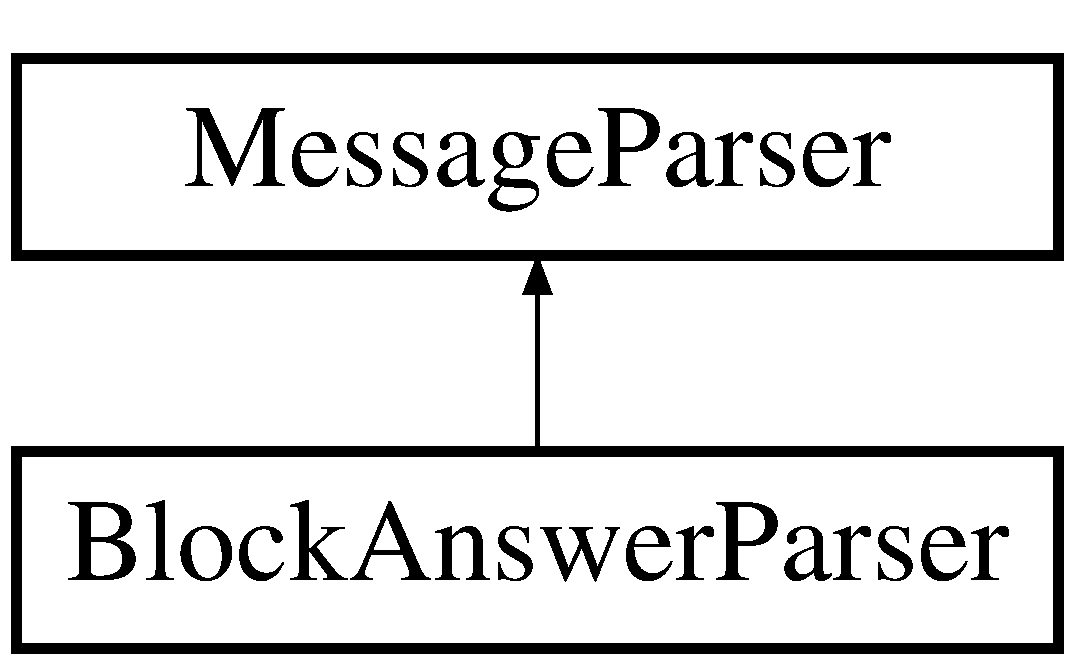
\includegraphics[height=2.000000cm]{classBlockAnswerParser}
\end{center}
\end{figure}
\subsection*{Public Member Functions}
\begin{DoxyCompactItemize}
\item 
void \mbox{\hyperlink{classBlockAnswerParser_a984cd68ad8878777f86cf6ed0892dd1d}{operator()}} (\mbox{\hyperlink{classMessage}{Message}} $\ast$m, \mbox{\hyperlink{classNode}{Node}} $\ast$node) const final
\item 
int \mbox{\hyperlink{classBlockAnswerParser_af29553ca77e4879f40f60a871105b6d4}{get\+\_\+type}} () const final
\end{DoxyCompactItemize}


\subsection{Detailed Description}
A message parser linked to a \mbox{\hyperlink{classBlockAnswerMessage}{Block\+Answer\+Message}}. \begin{DoxySeeAlso}{See also}
\mbox{\hyperlink{classMessage}{Message}} 

\mbox{\hyperlink{classBlockAnswerMessage}{Block\+Answer\+Message}} 

\mbox{\hyperlink{classMessageParser}{Message\+Parser}}
\end{DoxySeeAlso}
\begin{DoxyAuthor}{Author}
Mathieu Lochet 
\end{DoxyAuthor}
\begin{DoxyVersion}{Version}
1 
\end{DoxyVersion}


\subsection{Member Function Documentation}
\mbox{\Hypertarget{classBlockAnswerParser_af29553ca77e4879f40f60a871105b6d4}\label{classBlockAnswerParser_af29553ca77e4879f40f60a871105b6d4}} 
\index{Block\+Answer\+Parser@{Block\+Answer\+Parser}!get\+\_\+type@{get\+\_\+type}}
\index{get\+\_\+type@{get\+\_\+type}!Block\+Answer\+Parser@{Block\+Answer\+Parser}}
\subsubsection{\texorpdfstring{get\+\_\+type()}{get\_type()}}
{\footnotesize\ttfamily int Block\+Answer\+Parser\+::get\+\_\+type (\begin{DoxyParamCaption}{ }\end{DoxyParamCaption}) const\hspace{0.3cm}{\ttfamily [final]}, {\ttfamily [virtual]}}

Get the type of message the parser is linked to \begin{DoxySeeAlso}{See also}
\mbox{\hyperlink{classMessage}{Message}} 
\end{DoxySeeAlso}


Implements \mbox{\hyperlink{classMessageParser_aa7c495d7b28a394e5752ca25ffff69d8}{Message\+Parser}}.

\mbox{\Hypertarget{classBlockAnswerParser_a984cd68ad8878777f86cf6ed0892dd1d}\label{classBlockAnswerParser_a984cd68ad8878777f86cf6ed0892dd1d}} 
\index{Block\+Answer\+Parser@{Block\+Answer\+Parser}!operator()@{operator()}}
\index{operator()@{operator()}!Block\+Answer\+Parser@{Block\+Answer\+Parser}}
\subsubsection{\texorpdfstring{operator()()}{operator()()}}
{\footnotesize\ttfamily void Block\+Answer\+Parser\+::operator() (\begin{DoxyParamCaption}\item[{\mbox{\hyperlink{classMessage}{Message}} $\ast$}]{m,  }\item[{\mbox{\hyperlink{classNode}{Node}} $\ast$}]{node }\end{DoxyParamCaption}) const\hspace{0.3cm}{\ttfamily [final]}, {\ttfamily [virtual]}}

Process the message \begin{DoxySeeAlso}{See also}
\mbox{\hyperlink{classMessage}{Message}} 

\mbox{\hyperlink{classNode}{Node}}
\end{DoxySeeAlso}

\begin{DoxyParams}{Parameters}
{\em m} & The received message \\
\hline
{\em node} & The peer receiving the message \\
\hline
\end{DoxyParams}


Implements \mbox{\hyperlink{classMessageParser_a946f3b936dc01a75d6165329b159ecfe}{Message\+Parser}}.



The documentation for this class was generated from the following files\+:\begin{DoxyCompactItemize}
\item 
block\+\_\+chain/kernel/parsers/Block\+Answer\+Parser.\+h\item 
block\+\_\+chain/kernel/parsers/Block\+Answer\+Parser.\+cpp\end{DoxyCompactItemize}

\hypertarget{classBlockAskMessage}{}\section{Block\+Ask\+Message Class Reference}
\label{classBlockAskMessage}\index{Block\+Ask\+Message@{Block\+Ask\+Message}}


{\ttfamily \#include $<$Block\+Ask\+Message.\+h$>$}

Inheritance diagram for Block\+Ask\+Message\+:\begin{figure}[H]
\begin{center}
\leavevmode
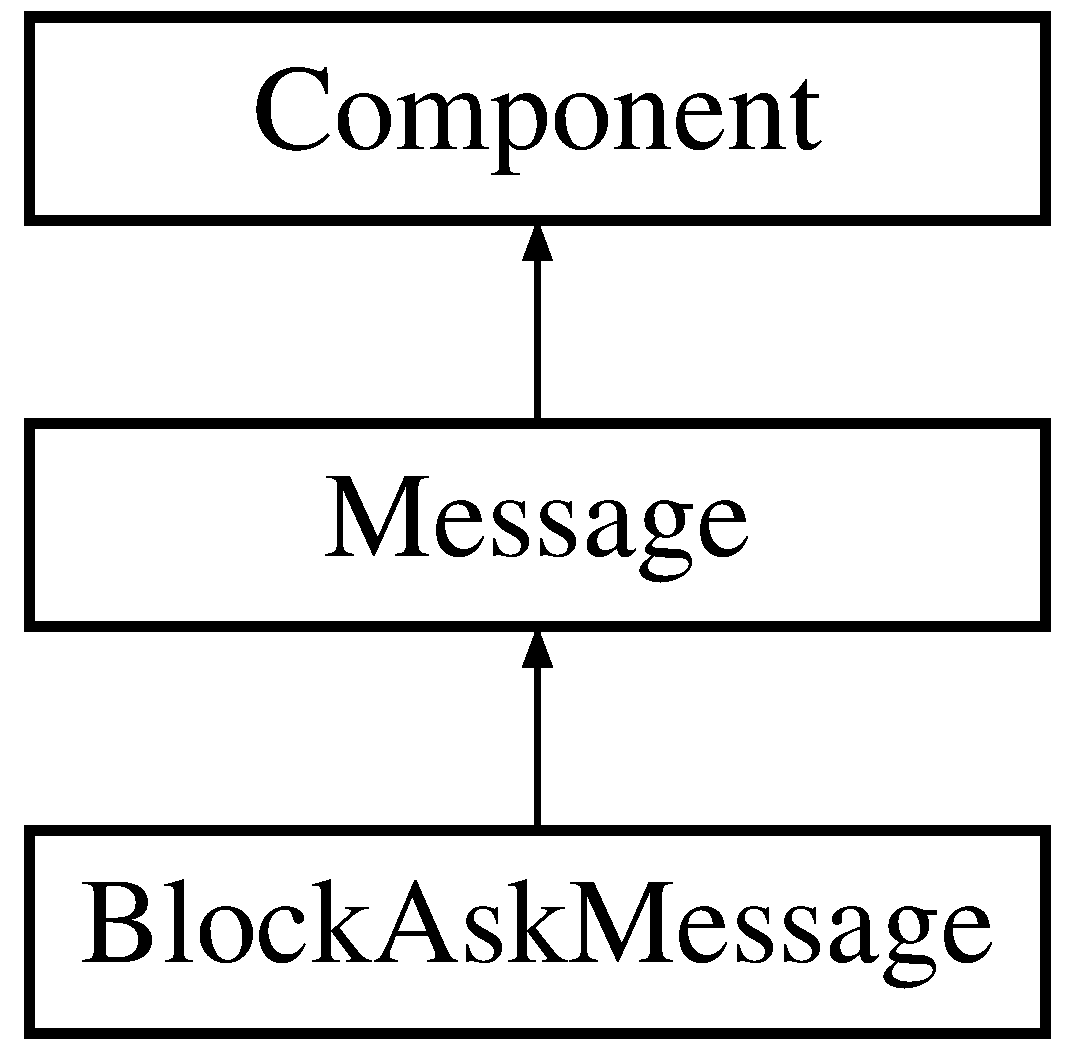
\includegraphics[height=3.000000cm]{classBlockAskMessage}
\end{center}
\end{figure}
\subsection*{Public Member Functions}
\begin{DoxyCompactItemize}
\item 
\mbox{\hyperlink{classBlockAskMessage_a21fd9feeb2fa7b306773c11cfaad7807}{Block\+Ask\+Message}} (std\+::string p, std\+::string f)
\item 
\mbox{\hyperlink{classElement}{Element}} $\ast$ \mbox{\hyperlink{classBlockAskMessage_a0bc20076f19423855ab5772003fb65f6}{to\+Element}} () const override
\item 
const int \mbox{\hyperlink{classMessage_a2a576dcffd45c4574fcdf2897ec26086}{get\+\_\+type}} () const
\item 
void \mbox{\hyperlink{classComponent_a28212595f8ee85fe009bd233bc99b2fc}{\+\_\+\+\_\+init\+\_\+\+\_\+}} (\mbox{\hyperlink{classElementObject}{Element\+Object}} $\ast$element, const \mbox{\hyperlink{classSerializer}{Serializer}} $\ast$s, const char $\ast$encoding)
\end{DoxyCompactItemize}
\subsection*{Static Public Member Functions}
\begin{DoxyCompactItemize}
\item 
static \mbox{\hyperlink{classMessage}{Message}} $\ast$ \mbox{\hyperlink{classMessage_ad92a0e1cfa5b5a503ec9c61833e3e5ea}{generate}} (int id)
\end{DoxyCompactItemize}
\subsection*{Static Public Attributes}
\begin{DoxyCompactItemize}
\item 
\mbox{\Hypertarget{classMessage_a18a7a0d3879210c798f3d84c820f03c1}\label{classMessage_a18a7a0d3879210c798f3d84c820f03c1}} 
static const int {\bfseries T\+R\+A\+N\+S\+A\+C\+T\+I\+ON} = 4
\item 
\mbox{\Hypertarget{classMessage_a3d3ef3111518cd65c0b7f5ec6660888a}\label{classMessage_a3d3ef3111518cd65c0b7f5ec6660888a}} 
static const int {\bfseries B\+L\+O\+CK} = 5
\item 
\mbox{\Hypertarget{classMessage_a9810d3cefb1b33e709cb393583a7a877}\label{classMessage_a9810d3cefb1b33e709cb393583a7a877}} 
static const int {\bfseries A\+S\+K\+\_\+\+P\+E\+E\+RS} = 0
\item 
\mbox{\Hypertarget{classMessage_aa33f42e5795c4df01c7437961d512eaa}\label{classMessage_aa33f42e5795c4df01c7437961d512eaa}} 
static const int {\bfseries A\+N\+S\+W\+E\+R\+\_\+\+P\+E\+E\+RS} = 1
\item 
\mbox{\Hypertarget{classMessage_a64b7688dfdd50a6254bf45b51d2118d4}\label{classMessage_a64b7688dfdd50a6254bf45b51d2118d4}} 
static const int {\bfseries S\+I\+G\+N\+\_\+\+IN} = 2
\item 
\mbox{\Hypertarget{classMessage_aba70c352293fee66004d729ccef3ee48}\label{classMessage_aba70c352293fee66004d729ccef3ee48}} 
static const int {\bfseries S\+I\+G\+N\+\_\+\+O\+UT} = 3
\item 
\mbox{\Hypertarget{classMessage_a62ac5b91838e79a11079869015261e14}\label{classMessage_a62ac5b91838e79a11079869015261e14}} 
static const int {\bfseries A\+S\+K\+\_\+\+B\+L\+O\+CK} = 6
\item 
\mbox{\Hypertarget{classMessage_a1580f4a26d125f71e2af1ef6001ac656}\label{classMessage_a1580f4a26d125f71e2af1ef6001ac656}} 
static const int {\bfseries A\+N\+S\+W\+E\+R\+\_\+\+B\+L\+O\+CK} = 7
\end{DoxyCompactItemize}
\subsection*{Protected Member Functions}
\begin{DoxyCompactItemize}
\item 
void \mbox{\hyperlink{classBlockAskMessage_a25875b2446d7ecc5f644c568c8f12df3}{from\+Element}} (\mbox{\hyperlink{classElementObject}{Element\+Object}} $\ast$, const \mbox{\hyperlink{classSerializer}{Serializer}} $\ast$serializer, const char $\ast$encoding) override
\end{DoxyCompactItemize}
\subsection*{Protected Attributes}
\begin{DoxyCompactItemize}
\item 
int \mbox{\hyperlink{classMessage_afbfb481c98b13d0deba0bac443bebe29}{type}}
\end{DoxyCompactItemize}
\subsection*{Friends}
\begin{DoxyCompactItemize}
\item 
\mbox{\Hypertarget{classBlockAskMessage_a8400d228b4c8e958886ed78dbbce07cf}\label{classBlockAskMessage_a8400d228b4c8e958886ed78dbbce07cf}} 
class {\bfseries Block\+Ask\+Parser}
\end{DoxyCompactItemize}


\subsection{Detailed Description}
A message to ask a missing block \begin{DoxySeeAlso}{See also}
\mbox{\hyperlink{classMessage}{Message}}
\end{DoxySeeAlso}
\begin{DoxyAuthor}{Author}
Mathieu Lochet 
\end{DoxyAuthor}
\begin{DoxyVersion}{Version}
1 
\end{DoxyVersion}


\subsection{Constructor \& Destructor Documentation}
\mbox{\Hypertarget{classBlockAskMessage_a21fd9feeb2fa7b306773c11cfaad7807}\label{classBlockAskMessage_a21fd9feeb2fa7b306773c11cfaad7807}} 
\index{Block\+Ask\+Message@{Block\+Ask\+Message}!Block\+Ask\+Message@{Block\+Ask\+Message}}
\index{Block\+Ask\+Message@{Block\+Ask\+Message}!Block\+Ask\+Message@{Block\+Ask\+Message}}
\subsubsection{\texorpdfstring{Block\+Ask\+Message()}{BlockAskMessage()}}
{\footnotesize\ttfamily Block\+Ask\+Message\+::\+Block\+Ask\+Message (\begin{DoxyParamCaption}\item[{std\+::string}]{p,  }\item[{std\+::string}]{f }\end{DoxyParamCaption})}

Creates a request for a missing block Calls the super constructor with the type value \begin{DoxySeeAlso}{See also}
Message\+::\+A\+S\+K\+\_\+\+B\+L\+O\+CK
\end{DoxySeeAlso}

\begin{DoxyParams}{Parameters}
{\em p} & The peer string representation \\
\hline
{\em f} & The fingerprint of the missing block \\
\hline
\end{DoxyParams}


\subsection{Member Function Documentation}
\mbox{\Hypertarget{classComponent_a28212595f8ee85fe009bd233bc99b2fc}\label{classComponent_a28212595f8ee85fe009bd233bc99b2fc}} 
\index{Block\+Ask\+Message@{Block\+Ask\+Message}!\+\_\+\+\_\+init\+\_\+\+\_\+@{\+\_\+\+\_\+init\+\_\+\+\_\+}}
\index{\+\_\+\+\_\+init\+\_\+\+\_\+@{\+\_\+\+\_\+init\+\_\+\+\_\+}!Block\+Ask\+Message@{Block\+Ask\+Message}}
\subsubsection{\texorpdfstring{\+\_\+\+\_\+init\+\_\+\+\_\+()}{\_\_init\_\_()}}
{\footnotesize\ttfamily void Component\+::\+\_\+\+\_\+init\+\_\+\+\_\+ (\begin{DoxyParamCaption}\item[{\mbox{\hyperlink{classElementObject}{Element\+Object}} $\ast$}]{element,  }\item[{const \mbox{\hyperlink{classSerializer}{Serializer}} $\ast$}]{s,  }\item[{const char $\ast$}]{encoding }\end{DoxyParamCaption})\hspace{0.3cm}{\ttfamily [inline]}, {\ttfamily [inherited]}}

The function called by the serializer to initialize the object if it is empty \begin{DoxySeeAlso}{See also}
\mbox{\hyperlink{classElementObject}{Element\+Object}} 

\mbox{\hyperlink{classSerializer}{Serializer}}
\end{DoxySeeAlso}

\begin{DoxyParams}{Parameters}
{\em element} & The \mbox{\hyperlink{classElement}{Element}} representation of the object \\
\hline
{\em s} & The serializer (Can be used if serialization of some elements is needed) \\
\hline
{\em encoding} & The encoding that has been used to create the \mbox{\hyperlink{classElement}{Element}} representation of the object (Can be used if serialization of some elements is needed) \\
\hline
\end{DoxyParams}
\mbox{\Hypertarget{classBlockAskMessage_a25875b2446d7ecc5f644c568c8f12df3}\label{classBlockAskMessage_a25875b2446d7ecc5f644c568c8f12df3}} 
\index{Block\+Ask\+Message@{Block\+Ask\+Message}!from\+Element@{from\+Element}}
\index{from\+Element@{from\+Element}!Block\+Ask\+Message@{Block\+Ask\+Message}}
\subsubsection{\texorpdfstring{from\+Element()}{fromElement()}}
{\footnotesize\ttfamily void Block\+Ask\+Message\+::from\+Element (\begin{DoxyParamCaption}\item[{\mbox{\hyperlink{classElementObject}{Element\+Object}} $\ast$}]{,  }\item[{const \mbox{\hyperlink{classSerializer}{Serializer}} $\ast$}]{,  }\item[{const char $\ast$}]{encoding }\end{DoxyParamCaption})\hspace{0.3cm}{\ttfamily [override]}, {\ttfamily [protected]}, {\ttfamily [virtual]}}

The function used to build the object from its element representation. the object if it is empty \begin{DoxySeeAlso}{See also}
\mbox{\hyperlink{classElementObject}{Element\+Object}} 

\mbox{\hyperlink{classSerializer}{Serializer}}
\end{DoxySeeAlso}

\begin{DoxyParams}{Parameters}
{\em element} & The \mbox{\hyperlink{classElement}{Element}} representation of the object \\
\hline
{\em s} & The serializer (Can be used if serialization of some elements is needed) \\
\hline
{\em encoding} & The encoding that has been used to create the \mbox{\hyperlink{classElement}{Element}} representation of the object (Can be used if serialization of some elements is needed) \\
\hline
\end{DoxyParams}


Implements \mbox{\hyperlink{classComponent_a2ded18881226d0077dc393e0e9304bb1}{Component}}.

\mbox{\Hypertarget{classMessage_ad92a0e1cfa5b5a503ec9c61833e3e5ea}\label{classMessage_ad92a0e1cfa5b5a503ec9c61833e3e5ea}} 
\index{Block\+Ask\+Message@{Block\+Ask\+Message}!generate@{generate}}
\index{generate@{generate}!Block\+Ask\+Message@{Block\+Ask\+Message}}
\subsubsection{\texorpdfstring{generate()}{generate()}}
{\footnotesize\ttfamily \mbox{\hyperlink{classMessage}{Message}} $\ast$ Message\+::generate (\begin{DoxyParamCaption}\item[{int}]{id }\end{DoxyParamCaption})\hspace{0.3cm}{\ttfamily [static]}, {\ttfamily [inherited]}}

The message factory\+: creates the corresponding type of message with a given type. The generated message is empty and needs to be fill. \begin{DoxySeeAlso}{See also}
\mbox{\hyperlink{classComponent}{Component}}\+:\+:{\bfseries init}
\end{DoxySeeAlso}

\begin{DoxyParams}{Parameters}
{\em id} & the given type of the wanted message \\
\hline
\end{DoxyParams}
\begin{DoxyReturn}{Returns}
The type of the message 
\end{DoxyReturn}
\mbox{\Hypertarget{classMessage_a2a576dcffd45c4574fcdf2897ec26086}\label{classMessage_a2a576dcffd45c4574fcdf2897ec26086}} 
\index{Block\+Ask\+Message@{Block\+Ask\+Message}!get\+\_\+type@{get\+\_\+type}}
\index{get\+\_\+type@{get\+\_\+type}!Block\+Ask\+Message@{Block\+Ask\+Message}}
\subsubsection{\texorpdfstring{get\+\_\+type()}{get\_type()}}
{\footnotesize\ttfamily const int Message\+::get\+\_\+type (\begin{DoxyParamCaption}{ }\end{DoxyParamCaption}) const\hspace{0.3cm}{\ttfamily [inherited]}}

Get the type of the message

\begin{DoxyReturn}{Returns}
The type of the message 
\end{DoxyReturn}
\mbox{\Hypertarget{classBlockAskMessage_a0bc20076f19423855ab5772003fb65f6}\label{classBlockAskMessage_a0bc20076f19423855ab5772003fb65f6}} 
\index{Block\+Ask\+Message@{Block\+Ask\+Message}!to\+Element@{to\+Element}}
\index{to\+Element@{to\+Element}!Block\+Ask\+Message@{Block\+Ask\+Message}}
\subsubsection{\texorpdfstring{to\+Element()}{toElement()}}
{\footnotesize\ttfamily \mbox{\hyperlink{classElement}{Element}} $\ast$ Block\+Ask\+Message\+::to\+Element (\begin{DoxyParamCaption}{ }\end{DoxyParamCaption}) const\hspace{0.3cm}{\ttfamily [override]}, {\ttfamily [virtual]}}

The method used by the serializer to transform an object into an \mbox{\hyperlink{classElement}{Element}} representation. \begin{DoxySeeAlso}{See also}
\mbox{\hyperlink{classElement}{Element}}
\end{DoxySeeAlso}
\begin{DoxyReturn}{Returns}
The \mbox{\hyperlink{classElement}{Element}} representation of the object 
\end{DoxyReturn}


Implements \mbox{\hyperlink{classComponent_a3e63d8c993e417a4af3f56d65ebfc7ea}{Component}}.



\subsection{Member Data Documentation}
\mbox{\Hypertarget{classMessage_afbfb481c98b13d0deba0bac443bebe29}\label{classMessage_afbfb481c98b13d0deba0bac443bebe29}} 
\index{Block\+Ask\+Message@{Block\+Ask\+Message}!type@{type}}
\index{type@{type}!Block\+Ask\+Message@{Block\+Ask\+Message}}
\subsubsection{\texorpdfstring{type}{type}}
{\footnotesize\ttfamily int Message\+::type\hspace{0.3cm}{\ttfamily [protected]}, {\ttfamily [inherited]}}

The type of the message 

The documentation for this class was generated from the following files\+:\begin{DoxyCompactItemize}
\item 
block\+\_\+chain/kernel/messages/Block\+Ask\+Message.\+h\item 
block\+\_\+chain/kernel/messages/Block\+Ask\+Message.\+cpp\end{DoxyCompactItemize}

\hypertarget{classBlockAskParser}{}\section{Block\+Ask\+Parser Class Reference}
\label{classBlockAskParser}\index{Block\+Ask\+Parser@{Block\+Ask\+Parser}}


{\ttfamily \#include $<$Block\+Ask\+Parser.\+h$>$}

Inheritance diagram for Block\+Ask\+Parser\+:\begin{figure}[H]
\begin{center}
\leavevmode
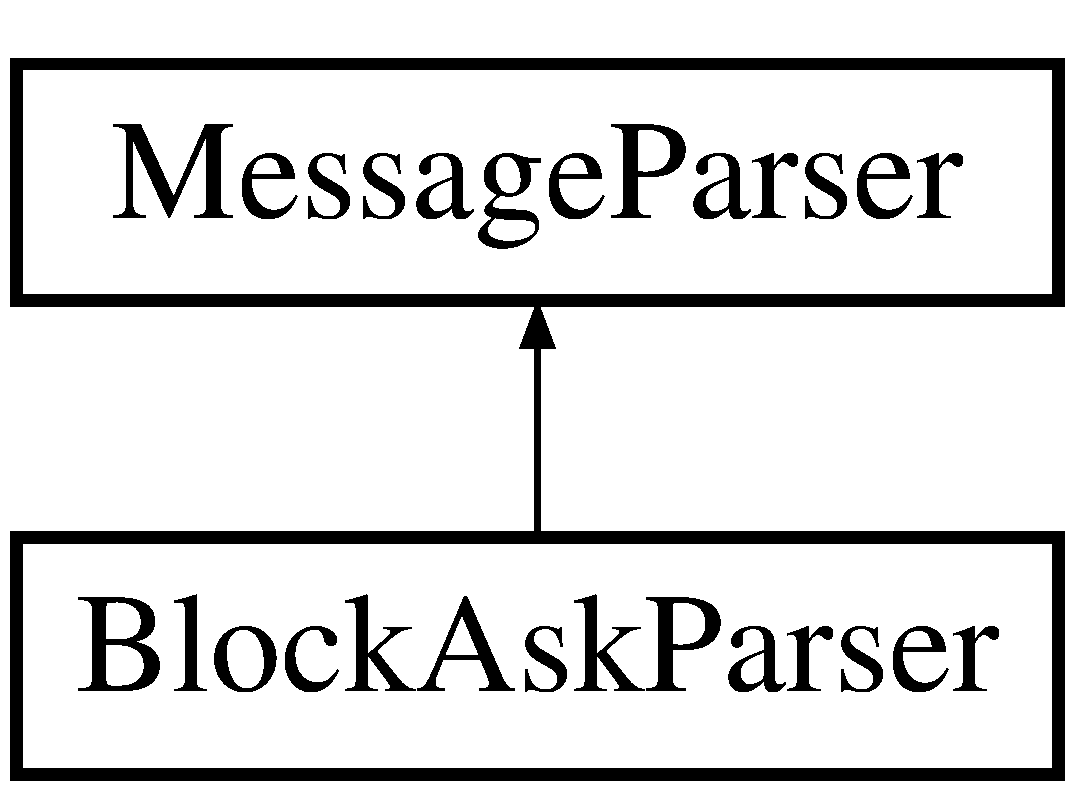
\includegraphics[height=2.000000cm]{classBlockAskParser}
\end{center}
\end{figure}
\subsection*{Public Member Functions}
\begin{DoxyCompactItemize}
\item 
void \mbox{\hyperlink{classBlockAskParser_a32d280786db26389f58175681ba35261}{operator()}} (\mbox{\hyperlink{classMessage}{Message}} $\ast$m, \mbox{\hyperlink{classNode}{Node}} $\ast$node) const final
\item 
int \mbox{\hyperlink{classBlockAskParser_add75da897c34702c33790947c9754500}{get\+\_\+type}} () const final
\end{DoxyCompactItemize}


\subsection{Detailed Description}
A message parser linked to a \mbox{\hyperlink{classBlockAskMessage}{Block\+Ask\+Message}}. \begin{DoxySeeAlso}{See also}
\mbox{\hyperlink{classMessage}{Message}} 

\mbox{\hyperlink{classBlockAskMessage}{Block\+Ask\+Message}} 

\mbox{\hyperlink{classMessageParser}{Message\+Parser}}
\end{DoxySeeAlso}
\begin{DoxyAuthor}{Author}
Mathieu Lochet 
\end{DoxyAuthor}
\begin{DoxyVersion}{Version}
1 
\end{DoxyVersion}


\subsection{Member Function Documentation}
\mbox{\Hypertarget{classBlockAskParser_add75da897c34702c33790947c9754500}\label{classBlockAskParser_add75da897c34702c33790947c9754500}} 
\index{Block\+Ask\+Parser@{Block\+Ask\+Parser}!get\+\_\+type@{get\+\_\+type}}
\index{get\+\_\+type@{get\+\_\+type}!Block\+Ask\+Parser@{Block\+Ask\+Parser}}
\subsubsection{\texorpdfstring{get\+\_\+type()}{get\_type()}}
{\footnotesize\ttfamily int Block\+Ask\+Parser\+::get\+\_\+type (\begin{DoxyParamCaption}{ }\end{DoxyParamCaption}) const\hspace{0.3cm}{\ttfamily [final]}, {\ttfamily [virtual]}}

Get the type of message the parser is linked to \begin{DoxySeeAlso}{See also}
\mbox{\hyperlink{classMessage}{Message}} 
\end{DoxySeeAlso}


Implements \mbox{\hyperlink{classMessageParser_aa7c495d7b28a394e5752ca25ffff69d8}{Message\+Parser}}.

\mbox{\Hypertarget{classBlockAskParser_a32d280786db26389f58175681ba35261}\label{classBlockAskParser_a32d280786db26389f58175681ba35261}} 
\index{Block\+Ask\+Parser@{Block\+Ask\+Parser}!operator()@{operator()}}
\index{operator()@{operator()}!Block\+Ask\+Parser@{Block\+Ask\+Parser}}
\subsubsection{\texorpdfstring{operator()()}{operator()()}}
{\footnotesize\ttfamily void Block\+Ask\+Parser\+::operator() (\begin{DoxyParamCaption}\item[{\mbox{\hyperlink{classMessage}{Message}} $\ast$}]{m,  }\item[{\mbox{\hyperlink{classNode}{Node}} $\ast$}]{node }\end{DoxyParamCaption}) const\hspace{0.3cm}{\ttfamily [final]}, {\ttfamily [virtual]}}

Process the message \begin{DoxySeeAlso}{See also}
\mbox{\hyperlink{classMessage}{Message}} 

\mbox{\hyperlink{classNode}{Node}}
\end{DoxySeeAlso}

\begin{DoxyParams}{Parameters}
{\em m} & The received message \\
\hline
{\em node} & The peer receiving the message \\
\hline
\end{DoxyParams}


Implements \mbox{\hyperlink{classMessageParser_a946f3b936dc01a75d6165329b159ecfe}{Message\+Parser}}.



The documentation for this class was generated from the following files\+:\begin{DoxyCompactItemize}
\item 
block\+\_\+chain/kernel/parsers/Block\+Ask\+Parser.\+h\item 
block\+\_\+chain/kernel/parsers/Block\+Ask\+Parser.\+cpp\end{DoxyCompactItemize}

\hypertarget{classBlockMessage}{}\section{Block\+Message Class Reference}
\label{classBlockMessage}\index{Block\+Message@{Block\+Message}}
Inheritance diagram for Block\+Message\+:\begin{figure}[H]
\begin{center}
\leavevmode
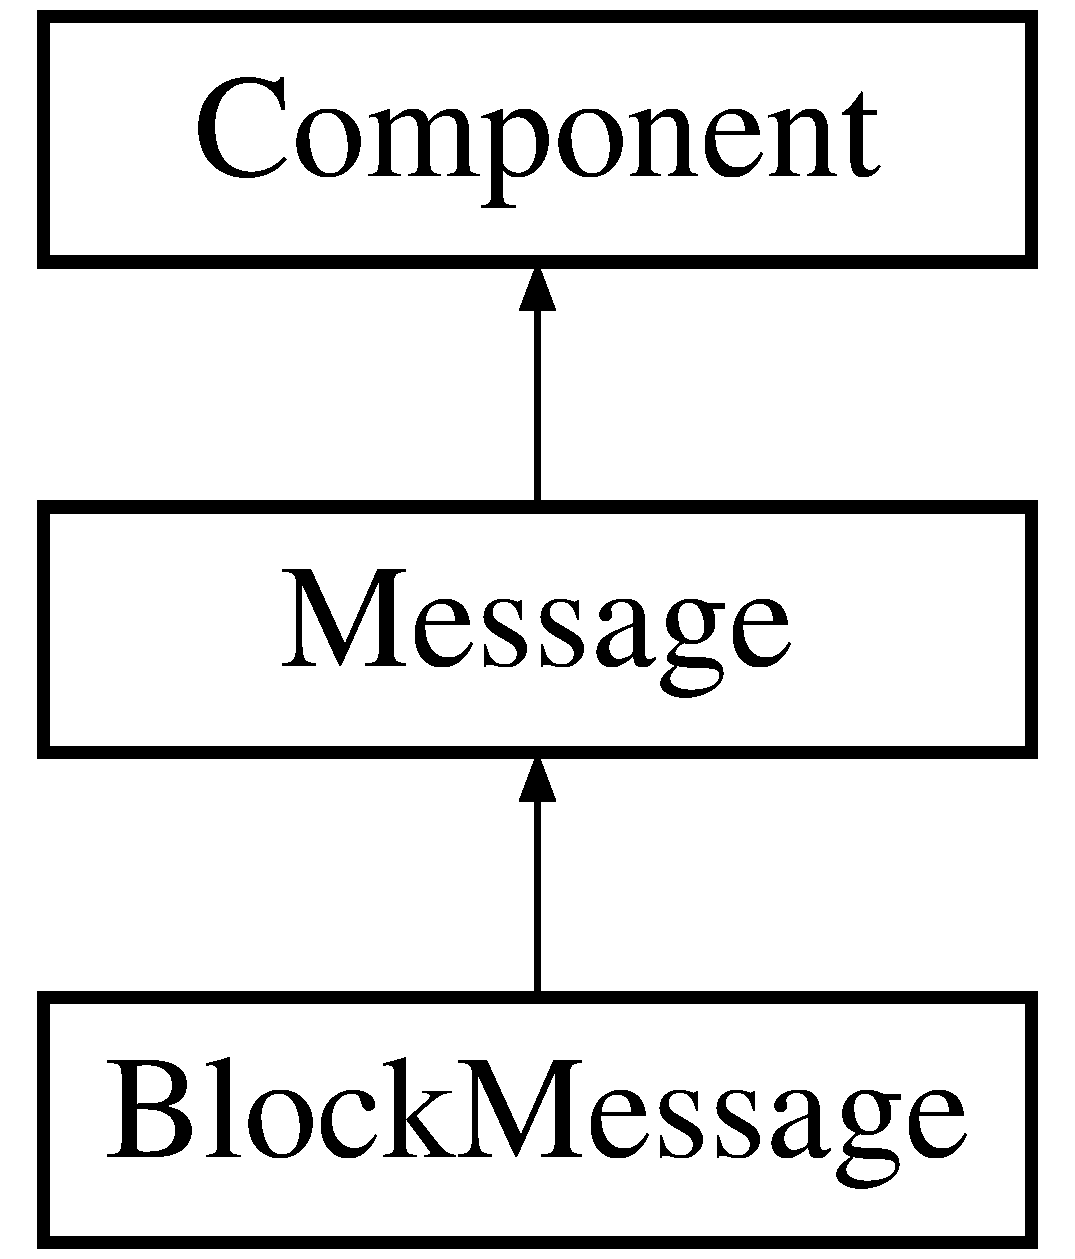
\includegraphics[height=3.000000cm]{classBlockMessage}
\end{center}
\end{figure}
\subsection*{Public Member Functions}
\begin{DoxyCompactItemize}
\item 
\mbox{\Hypertarget{classBlockMessage_a84debf84ee00990f2c279b40a3143db0}\label{classBlockMessage_a84debf84ee00990f2c279b40a3143db0}} 
{\bfseries Block\+Message} (std\+::string b, std\+::string k, \mbox{\hyperlink{classMerkleTree}{Merkle\+Tree}} $\ast$tr)
\item 
\mbox{\Hypertarget{classBlockMessage_ab47afd5cfb7d6d5c544d8def5d0f9737}\label{classBlockMessage_ab47afd5cfb7d6d5c544d8def5d0f9737}} 
\mbox{\hyperlink{classElement}{Element}} $\ast$ {\bfseries to\+Element} () const override
\item 
\mbox{\Hypertarget{classBlockMessage_a62842475d6d9d9b82806c3a90ed56123}\label{classBlockMessage_a62842475d6d9d9b82806c3a90ed56123}} 
const std\+::string {\bfseries get\+\_\+key} () const
\item 
\mbox{\Hypertarget{classMessage_a2a576dcffd45c4574fcdf2897ec26086}\label{classMessage_a2a576dcffd45c4574fcdf2897ec26086}} 
const int {\bfseries get\+\_\+type} () const
\item 
\mbox{\Hypertarget{classComponent_a28212595f8ee85fe009bd233bc99b2fc}\label{classComponent_a28212595f8ee85fe009bd233bc99b2fc}} 
void {\bfseries \+\_\+\+\_\+init\+\_\+\+\_\+} (\mbox{\hyperlink{classElementObject}{Element\+Object}} $\ast$element, const \mbox{\hyperlink{classSerializer}{Serializer}} $\ast$s, const char $\ast$encoding)
\end{DoxyCompactItemize}
\subsection*{Static Public Member Functions}
\begin{DoxyCompactItemize}
\item 
\mbox{\Hypertarget{classMessage_ad92a0e1cfa5b5a503ec9c61833e3e5ea}\label{classMessage_ad92a0e1cfa5b5a503ec9c61833e3e5ea}} 
static \mbox{\hyperlink{classMessage}{Message}} $\ast$ {\bfseries generate} (int id)
\end{DoxyCompactItemize}
\subsection*{Static Public Attributes}
\begin{DoxyCompactItemize}
\item 
\mbox{\Hypertarget{classMessage_a18a7a0d3879210c798f3d84c820f03c1}\label{classMessage_a18a7a0d3879210c798f3d84c820f03c1}} 
static const int {\bfseries T\+R\+A\+N\+S\+A\+C\+T\+I\+ON} = 4
\item 
\mbox{\Hypertarget{classMessage_a3d3ef3111518cd65c0b7f5ec6660888a}\label{classMessage_a3d3ef3111518cd65c0b7f5ec6660888a}} 
static const int {\bfseries B\+L\+O\+CK} = 5
\item 
\mbox{\Hypertarget{classMessage_a9810d3cefb1b33e709cb393583a7a877}\label{classMessage_a9810d3cefb1b33e709cb393583a7a877}} 
static const int {\bfseries A\+S\+K\+\_\+\+P\+E\+E\+RS} = 0
\item 
\mbox{\Hypertarget{classMessage_aa33f42e5795c4df01c7437961d512eaa}\label{classMessage_aa33f42e5795c4df01c7437961d512eaa}} 
static const int {\bfseries A\+N\+S\+W\+E\+R\+\_\+\+P\+E\+E\+RS} = 1
\item 
\mbox{\Hypertarget{classMessage_a64b7688dfdd50a6254bf45b51d2118d4}\label{classMessage_a64b7688dfdd50a6254bf45b51d2118d4}} 
static const int {\bfseries S\+I\+G\+N\+\_\+\+IN} = 2
\item 
\mbox{\Hypertarget{classMessage_aba70c352293fee66004d729ccef3ee48}\label{classMessage_aba70c352293fee66004d729ccef3ee48}} 
static const int {\bfseries S\+I\+G\+N\+\_\+\+O\+UT} = 3
\item 
\mbox{\Hypertarget{classMessage_a62ac5b91838e79a11079869015261e14}\label{classMessage_a62ac5b91838e79a11079869015261e14}} 
static const int {\bfseries A\+S\+K\+\_\+\+B\+L\+O\+CK} = 6
\item 
\mbox{\Hypertarget{classMessage_a1580f4a26d125f71e2af1ef6001ac656}\label{classMessage_a1580f4a26d125f71e2af1ef6001ac656}} 
static const int {\bfseries A\+N\+S\+W\+E\+R\+\_\+\+B\+L\+O\+CK} = 7
\end{DoxyCompactItemize}
\subsection*{Protected Member Functions}
\begin{DoxyCompactItemize}
\item 
\mbox{\Hypertarget{classBlockMessage_adda957e60057d72e1bc55d7b9c617188}\label{classBlockMessage_adda957e60057d72e1bc55d7b9c617188}} 
void {\bfseries from\+Element} (\mbox{\hyperlink{classElementObject}{Element\+Object}} $\ast$, const \mbox{\hyperlink{classSerializer}{Serializer}} $\ast$serializer, const char $\ast$encoding) override
\end{DoxyCompactItemize}
\subsection*{Protected Attributes}
\begin{DoxyCompactItemize}
\item 
\mbox{\Hypertarget{classMessage_afbfb481c98b13d0deba0bac443bebe29}\label{classMessage_afbfb481c98b13d0deba0bac443bebe29}} 
int {\bfseries type}
\end{DoxyCompactItemize}
\subsection*{Friends}
\begin{DoxyCompactItemize}
\item 
\mbox{\Hypertarget{classBlockMessage_a8428b3aeea6607d1ba12e603ff9d015c}\label{classBlockMessage_a8428b3aeea6607d1ba12e603ff9d015c}} 
class {\bfseries Block\+Parser}
\end{DoxyCompactItemize}


The documentation for this class was generated from the following files\+:\begin{DoxyCompactItemize}
\item 
block\+\_\+chain/kernel/messages/Block\+Message.\+h\item 
block\+\_\+chain/kernel/messages/Block\+Message.\+cpp\end{DoxyCompactItemize}

\hypertarget{classBlockParser}{}\section{Block\+Parser Class Reference}
\label{classBlockParser}\index{Block\+Parser@{Block\+Parser}}
Inheritance diagram for Block\+Parser\+:\begin{figure}[H]
\begin{center}
\leavevmode
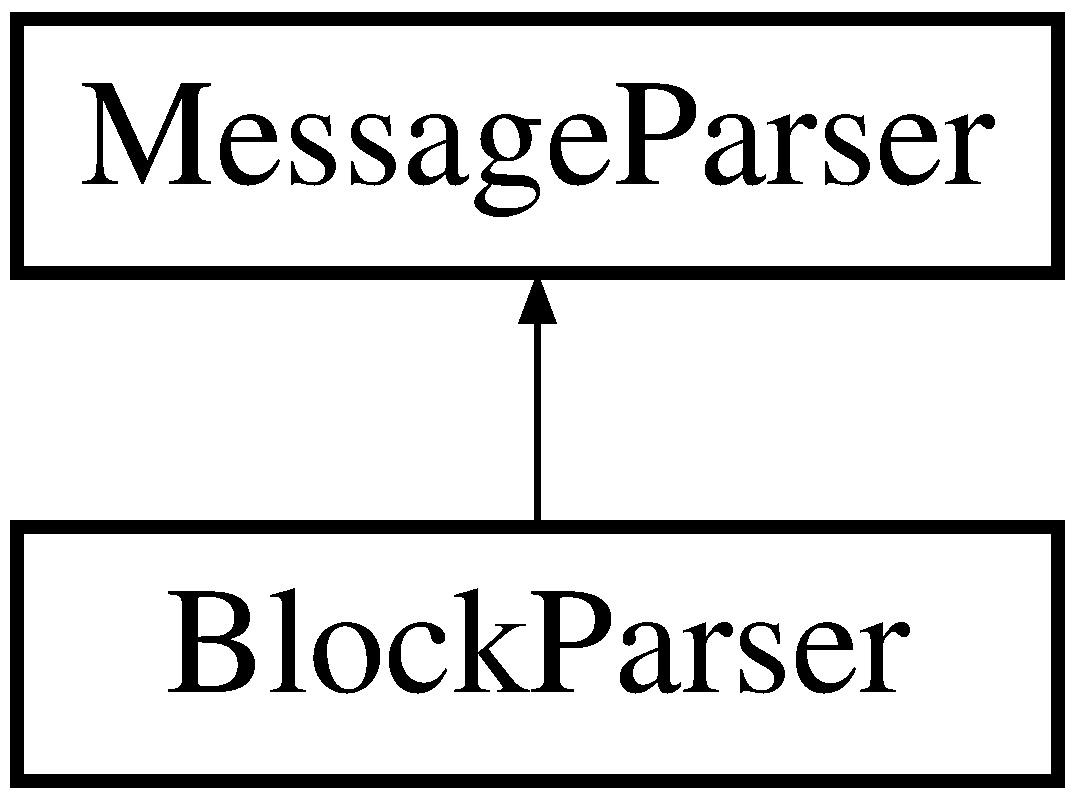
\includegraphics[height=2.000000cm]{classBlockParser}
\end{center}
\end{figure}
\subsection*{Public Member Functions}
\begin{DoxyCompactItemize}
\item 
\mbox{\Hypertarget{classBlockParser_acc2f5e6a6d3a30464454cfc85ff7ba9a}\label{classBlockParser_acc2f5e6a6d3a30464454cfc85ff7ba9a}} 
void {\bfseries operator()} (\mbox{\hyperlink{classMessage}{Message}} $\ast$m, \mbox{\hyperlink{classNode}{Node}} $\ast$node) const final
\item 
\mbox{\Hypertarget{classBlockParser_aa7334a81b976ec6244c0992cda44a824}\label{classBlockParser_aa7334a81b976ec6244c0992cda44a824}} 
int {\bfseries get\+\_\+type} () const final
\end{DoxyCompactItemize}


The documentation for this class was generated from the following files\+:\begin{DoxyCompactItemize}
\item 
block\+\_\+chain/kernel/parsers/Block\+Parser.\+h\item 
block\+\_\+chain/kernel/parsers/Block\+Parser.\+cpp\end{DoxyCompactItemize}

\hypertarget{classChain}{}\section{Chain Class Reference}
\label{classChain}\index{Chain@{Chain}}
\subsection*{Public Member Functions}
\begin{DoxyCompactItemize}
\item 
\mbox{\Hypertarget{classChain_a851466afd0f86ef862ce36dd287546bf}\label{classChain_a851466afd0f86ef862ce36dd287546bf}} 
{\bfseries Chain} (\mbox{\hyperlink{classBlock}{Block}} $\ast$, \mbox{\hyperlink{classChain}{Chain}} $\ast$c)
\item 
\mbox{\Hypertarget{classChain_a6779b5168023552f943c54baed7e7cd4}\label{classChain_a6779b5168023552f943c54baed7e7cd4}} 
{\bfseries Chain} (\mbox{\hyperlink{classReward}{Reward}} $\ast$r)
\item 
\mbox{\Hypertarget{classChain_a1a8b5c5196b8b1c50f54349755721932}\label{classChain_a1a8b5c5196b8b1c50f54349755721932}} 
void {\bfseries add} (\mbox{\hyperlink{classBlock}{Block}} $\ast$)
\item 
\mbox{\Hypertarget{classChain_a5ee2e1efbfe8d2896b0ac836fb750362}\label{classChain_a5ee2e1efbfe8d2896b0ac836fb750362}} 
std\+::pair$<$ int, \mbox{\hyperlink{classChain}{Chain}} $\ast$ $>$ {\bfseries top\+\_\+fingerprint} ()
\item 
\mbox{\Hypertarget{classChain_abeec0de116c442e6da59230a85a56724}\label{classChain_abeec0de116c442e6da59230a85a56724}} 
void {\bfseries update\+\_\+database} (\mbox{\hyperlink{classBlock}{Block}} $\ast$, const \mbox{\hyperlink{classSerializer}{Serializer}} $\ast$s, const char $\ast$encoding)
\item 
\mbox{\Hypertarget{classChain_a5725ffa89b1f0333536238951d9acd91}\label{classChain_a5725ffa89b1f0333536238951d9acd91}} 
bool {\bfseries check\+\_\+transaction} (\mbox{\hyperlink{classTransaction}{Transaction}} $\ast$transaction, std\+::string k)
\item 
\mbox{\Hypertarget{classChain_ad06a7e312123831339b614a74ff5c9e0}\label{classChain_ad06a7e312123831339b614a74ff5c9e0}} 
int {\bfseries count} () const
\end{DoxyCompactItemize}
\subsection*{Friends}
\begin{DoxyCompactItemize}
\item 
\mbox{\Hypertarget{classChain_adfdd1242f00ef4da9a9a01d996fc292c}\label{classChain_adfdd1242f00ef4da9a9a01d996fc292c}} 
class {\bfseries Node\+State}
\end{DoxyCompactItemize}


The documentation for this class was generated from the following files\+:\begin{DoxyCompactItemize}
\item 
block\+\_\+chain/chain/Chain.\+h\item 
block\+\_\+chain/chain/Chain.\+cpp\end{DoxyCompactItemize}

\hypertarget{classComponent}{}\section{Component Class Reference}
\label{classComponent}\index{Component@{Component}}


{\ttfamily \#include $<$Component.\+h$>$}

Inheritance diagram for Component\+:\begin{figure}[H]
\begin{center}
\leavevmode
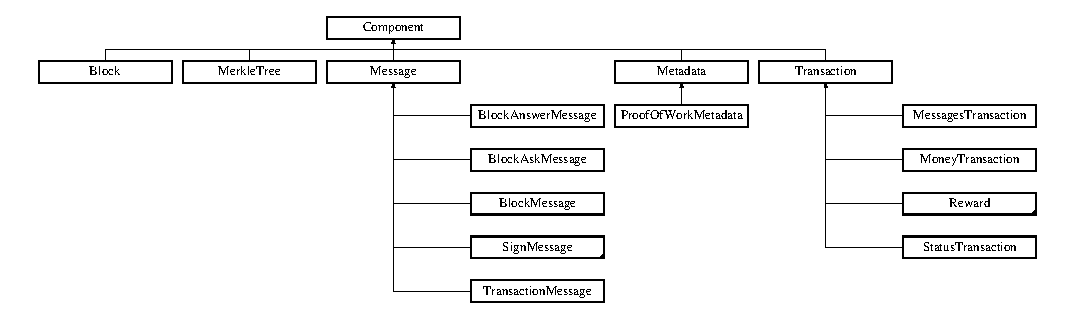
\includegraphics[height=3.835616cm]{classComponent}
\end{center}
\end{figure}
\subsection*{Public Member Functions}
\begin{DoxyCompactItemize}
\item 
virtual \mbox{\hyperlink{classComponent_ab8378fa275af98e568a7e91d33d867af}{$\sim$\+Component}} ()
\item 
\mbox{\hyperlink{classComponent_a8775db6d1a2c1afc2e77cd3c8f39da6f}{Component}} ()
\item 
virtual \mbox{\hyperlink{classElement}{Element}} $\ast$ \mbox{\hyperlink{classComponent_a3e63d8c993e417a4af3f56d65ebfc7ea}{to\+Element}} () const =0
\item 
void \mbox{\hyperlink{classComponent_a28212595f8ee85fe009bd233bc99b2fc}{\+\_\+\+\_\+init\+\_\+\+\_\+}} (\mbox{\hyperlink{classElementObject}{Element\+Object}} $\ast$element, const \mbox{\hyperlink{classSerializer}{Serializer}} $\ast$s, const char $\ast$encoding)
\end{DoxyCompactItemize}
\subsection*{Protected Member Functions}
\begin{DoxyCompactItemize}
\item 
virtual void \mbox{\hyperlink{classComponent_a2ded18881226d0077dc393e0e9304bb1}{from\+Element}} (\mbox{\hyperlink{classElementObject}{Element\+Object}} $\ast$, const \mbox{\hyperlink{classSerializer}{Serializer}} $\ast$, const char $\ast$encoding)=0
\end{DoxyCompactItemize}


\subsection{Detailed Description}
The main abstract class for serialization. All possible classes that can be serialized need to implement this interface. \begin{DoxySeeAlso}{See also}
\mbox{\hyperlink{classSerializer}{Serializer}}
\end{DoxySeeAlso}
\begin{DoxyAuthor}{Author}
Mathieu Lochet 
\end{DoxyAuthor}
\begin{DoxyVersion}{Version}
1 
\end{DoxyVersion}


\subsection{Constructor \& Destructor Documentation}
\mbox{\Hypertarget{classComponent_ab8378fa275af98e568a7e91d33d867af}\label{classComponent_ab8378fa275af98e568a7e91d33d867af}} 
\index{Component@{Component}!````~Component@{$\sim$\+Component}}
\index{````~Component@{$\sim$\+Component}!Component@{Component}}
\subsubsection{\texorpdfstring{$\sim$\+Component()}{~Component()}}
{\footnotesize\ttfamily Component\+::$\sim$\+Component (\begin{DoxyParamCaption}{ }\end{DoxyParamCaption})\hspace{0.3cm}{\ttfamily [virtual]}, {\ttfamily [default]}}

A default virtual destructor \mbox{\Hypertarget{classComponent_a8775db6d1a2c1afc2e77cd3c8f39da6f}\label{classComponent_a8775db6d1a2c1afc2e77cd3c8f39da6f}} 
\index{Component@{Component}!Component@{Component}}
\index{Component@{Component}!Component@{Component}}
\subsubsection{\texorpdfstring{Component()}{Component()}}
{\footnotesize\ttfamily Component\+::\+Component (\begin{DoxyParamCaption}{ }\end{DoxyParamCaption})\hspace{0.3cm}{\ttfamily [default]}}

A default constructor for initialization 

\subsection{Member Function Documentation}
\mbox{\Hypertarget{classComponent_a28212595f8ee85fe009bd233bc99b2fc}\label{classComponent_a28212595f8ee85fe009bd233bc99b2fc}} 
\index{Component@{Component}!\+\_\+\+\_\+init\+\_\+\+\_\+@{\+\_\+\+\_\+init\+\_\+\+\_\+}}
\index{\+\_\+\+\_\+init\+\_\+\+\_\+@{\+\_\+\+\_\+init\+\_\+\+\_\+}!Component@{Component}}
\subsubsection{\texorpdfstring{\+\_\+\+\_\+init\+\_\+\+\_\+()}{\_\_init\_\_()}}
{\footnotesize\ttfamily void Component\+::\+\_\+\+\_\+init\+\_\+\+\_\+ (\begin{DoxyParamCaption}\item[{\mbox{\hyperlink{classElementObject}{Element\+Object}} $\ast$}]{element,  }\item[{const \mbox{\hyperlink{classSerializer}{Serializer}} $\ast$}]{s,  }\item[{const char $\ast$}]{encoding }\end{DoxyParamCaption})\hspace{0.3cm}{\ttfamily [inline]}}

The function called by the serializer to initialize the object if it is empty \begin{DoxySeeAlso}{See also}
\mbox{\hyperlink{classElementObject}{Element\+Object}} 

\mbox{\hyperlink{classSerializer}{Serializer}}
\end{DoxySeeAlso}

\begin{DoxyParams}{Parameters}
{\em element} & The \mbox{\hyperlink{classElement}{Element}} representation of the object \\
\hline
{\em s} & The serializer (Can be used if serialization of some elements is needed) \\
\hline
{\em encoding} & The encoding that has been used to create the \mbox{\hyperlink{classElement}{Element}} representation of the object (Can be used if serialization of some elements is needed) \\
\hline
\end{DoxyParams}
\mbox{\Hypertarget{classComponent_a2ded18881226d0077dc393e0e9304bb1}\label{classComponent_a2ded18881226d0077dc393e0e9304bb1}} 
\index{Component@{Component}!from\+Element@{from\+Element}}
\index{from\+Element@{from\+Element}!Component@{Component}}
\subsubsection{\texorpdfstring{from\+Element()}{fromElement()}}
{\footnotesize\ttfamily virtual void Component\+::from\+Element (\begin{DoxyParamCaption}\item[{\mbox{\hyperlink{classElementObject}{Element\+Object}} $\ast$}]{,  }\item[{const \mbox{\hyperlink{classSerializer}{Serializer}} $\ast$}]{,  }\item[{const char $\ast$}]{encoding }\end{DoxyParamCaption})\hspace{0.3cm}{\ttfamily [protected]}, {\ttfamily [pure virtual]}}

The function used to build the object from its element representation. the object if it is empty \begin{DoxySeeAlso}{See also}
\mbox{\hyperlink{classElementObject}{Element\+Object}} 

\mbox{\hyperlink{classSerializer}{Serializer}}
\end{DoxySeeAlso}

\begin{DoxyParams}{Parameters}
{\em element} & The \mbox{\hyperlink{classElement}{Element}} representation of the object \\
\hline
{\em s} & The serializer (Can be used if serialization of some elements is needed) \\
\hline
{\em encoding} & The encoding that has been used to create the \mbox{\hyperlink{classElement}{Element}} representation of the object (Can be used if serialization of some elements is needed) \\
\hline
\end{DoxyParams}


Implemented in \mbox{\hyperlink{classMerkleTree_a083ad348bfd770f2400f190112ff39a3}{Merkle\+Tree}}, \mbox{\hyperlink{classBlock_ab21c6536cf7a26fdf2a2e889a84fcb9d}{Block}}, \mbox{\hyperlink{classTransactionMessage_a2fbe322d67154d3bcbcc44943eeeb1ef}{Transaction\+Message}}, \mbox{\hyperlink{classBlockMessage_adda957e60057d72e1bc55d7b9c617188}{Block\+Message}}, \mbox{\hyperlink{classProofOfWorkMetadata_afac533eee3123bce72615ab90f7c9669}{Proof\+Of\+Work\+Metadata}}, \mbox{\hyperlink{classSignMessage_a35855647925ec76036ed4602743ed118}{Sign\+Message}}, \mbox{\hyperlink{classMessagesTransaction_aa70ed75ff16f6afa61d82458488069d4}{Messages\+Transaction}}, \mbox{\hyperlink{classReward_a6d16e21b60b7f11c7aaf0098a53118a2}{Reward}}, \mbox{\hyperlink{classMoneyTransaction_a6f4672dba3a75e2782d15366d9ed7a1e}{Money\+Transaction}}, \mbox{\hyperlink{classBlockAskMessage_a25875b2446d7ecc5f644c568c8f12df3}{Block\+Ask\+Message}}, \mbox{\hyperlink{classBlockAnswerMessage_affa76e8a95365baf5c9eb409a0a19b9d}{Block\+Answer\+Message}}, and \mbox{\hyperlink{classStatusTransaction_aa05e4be5f990e8a9533383b3b7dc1382}{Status\+Transaction}}.

\mbox{\Hypertarget{classComponent_a3e63d8c993e417a4af3f56d65ebfc7ea}\label{classComponent_a3e63d8c993e417a4af3f56d65ebfc7ea}} 
\index{Component@{Component}!to\+Element@{to\+Element}}
\index{to\+Element@{to\+Element}!Component@{Component}}
\subsubsection{\texorpdfstring{to\+Element()}{toElement()}}
{\footnotesize\ttfamily virtual \mbox{\hyperlink{classElement}{Element}}$\ast$ Component\+::to\+Element (\begin{DoxyParamCaption}{ }\end{DoxyParamCaption}) const\hspace{0.3cm}{\ttfamily [pure virtual]}}

The method used by the serializer to transform an object into an \mbox{\hyperlink{classElement}{Element}} representation. \begin{DoxySeeAlso}{See also}
\mbox{\hyperlink{classElement}{Element}}
\end{DoxySeeAlso}
\begin{DoxyReturn}{Returns}
The \mbox{\hyperlink{classElement}{Element}} representation of the object 
\end{DoxyReturn}


Implemented in \mbox{\hyperlink{classMerkleTree_a4e72819c6cbc49ed8ce092f464711a5f}{Merkle\+Tree}}, \mbox{\hyperlink{classBlock_aa289363a40f0d3ba88720ad0bc71f34f}{Block}}, \mbox{\hyperlink{classTransactionMessage_ae20e7d6a7b5811bb56a32ec6af59b8e2}{Transaction\+Message}}, \mbox{\hyperlink{classBlockMessage_ab47afd5cfb7d6d5c544d8def5d0f9737}{Block\+Message}}, \mbox{\hyperlink{classSignMessage_aee897c4bf78df966b8cca95e589566e4}{Sign\+Message}}, \mbox{\hyperlink{classProofOfWorkMetadata_a2aab4c26afb3a85a712cc065028274d9}{Proof\+Of\+Work\+Metadata}}, \mbox{\hyperlink{classBlockAskMessage_a0bc20076f19423855ab5772003fb65f6}{Block\+Ask\+Message}}, \mbox{\hyperlink{classBlockAnswerMessage_ac7f35ec9f7f2fbcd726628c2a984518b}{Block\+Answer\+Message}}, \mbox{\hyperlink{classReward_a0ecd536148463880f9980fe415b6eb1d}{Reward}}, \mbox{\hyperlink{classMessagesTransaction_a0ef8ec080a2698a02ad8b1b95d243720}{Messages\+Transaction}}, \mbox{\hyperlink{classStatusTransaction_aed42f2d61f2d50ec07bb6b35473f61f2}{Status\+Transaction}}, and \mbox{\hyperlink{classMoneyTransaction_a84adc847266467965014cb04acd48bea}{Money\+Transaction}}.



The documentation for this class was generated from the following files\+:\begin{DoxyCompactItemize}
\item 
block\+\_\+chain/kernel/components/Component.\+h\item 
block\+\_\+chain/kernel/components/Component.\+cpp\end{DoxyCompactItemize}

\hypertarget{classConfig}{}\section{Config Class Reference}
\label{classConfig}\index{Config@{Config}}


{\ttfamily \#include $<$Config.\+h$>$}

\subsection*{Public Member Functions}
\begin{DoxyCompactItemize}
\item 
\mbox{\hyperlink{classConfig_a215344f9d1452f24df7c0508a23fd15b}{Config}} (const char $\ast$filename, \mbox{\hyperlink{classSerializer}{Serializer}} $\ast$s, int p, \mbox{\hyperlink{classReward}{Reward}} $\ast$r)
\item 
virtual const char $\ast$ \mbox{\hyperlink{classConfig_a23f39330cd594b8855d371368adc80e4}{get\+\_\+encoding}} () const
\item 
virtual const \mbox{\hyperlink{classSerializer}{Serializer}} $\ast$ \mbox{\hyperlink{classConfig_a00399f1751e2dfa032d99208bf925ab0}{get\+\_\+serializer}} () const
\item 
virtual const \mbox{\hyperlink{classProof}{Proof}} $\ast$ \mbox{\hyperlink{classConfig_a23b6ece178053913f232eeda4ab7c7c8}{get\+\_\+proof}} () const
\item 
virtual const \mbox{\hyperlink{classReward}{Reward}} $\ast$ \mbox{\hyperlink{classConfig_a3467e8914f0a0730277cf4732443116d}{get\+\_\+reward}} () const
\item 
virtual const int \mbox{\hyperlink{classConfig_a516e5e6665ad519ab23ac4c57fb99cb6}{get\+\_\+port}} () const
\item 
virtual const bool \mbox{\hyperlink{classConfig_afc60cc21dfa15f3642f8ac1f45403450}{is\+\_\+debug}} () const
\end{DoxyCompactItemize}
\subsection*{Protected Attributes}
\begin{DoxyCompactItemize}
\item 
int \mbox{\hyperlink{classConfig_a9b99e069f6e78fcb906d5effbb600e97}{port}}
\item 
std\+::string \mbox{\hyperlink{classConfig_a9391a8a86ed88a6fefd35ec89c10e861}{encoding}}
\item 
\mbox{\hyperlink{classSerializer}{Serializer}} $\ast$ \mbox{\hyperlink{classConfig_afcd74e506e51f57020bce34fe92cb9dc}{serializer}}
\item 
\mbox{\hyperlink{classProof}{Proof}} $\ast$ \mbox{\hyperlink{classConfig_ac220c43cceafde6291b29d44f61c3785}{proof}}
\item 
\mbox{\hyperlink{classReward}{Reward}} $\ast$ \mbox{\hyperlink{classConfig_a6b3fb8d8312246a1b204d04bd872a187}{reward}}
\item 
bool \mbox{\hyperlink{classConfig_a8ecbe763ad856693ff85cba5182e1f2e}{debug}}
\end{DoxyCompactItemize}


\subsection{Detailed Description}
The config is the object that contains all of the important data to run the program. \begin{DoxySeeAlso}{See also}
\mbox{\hyperlink{classSerializer}{Serializer}} 

\mbox{\hyperlink{classReward}{Reward}} 

\mbox{\hyperlink{classProof}{Proof}}
\end{DoxySeeAlso}
\begin{DoxyAuthor}{Author}
Mathieu Lochet 
\end{DoxyAuthor}
\begin{DoxyVersion}{Version}
1 
\end{DoxyVersion}


\subsection{Constructor \& Destructor Documentation}
\mbox{\Hypertarget{classConfig_a215344f9d1452f24df7c0508a23fd15b}\label{classConfig_a215344f9d1452f24df7c0508a23fd15b}} 
\index{Config@{Config}!Config@{Config}}
\index{Config@{Config}!Config@{Config}}
\subsubsection{\texorpdfstring{Config()}{Config()}}
{\footnotesize\ttfamily Config\+::\+Config (\begin{DoxyParamCaption}\item[{const char $\ast$}]{filename,  }\item[{\mbox{\hyperlink{classSerializer}{Serializer}} $\ast$}]{s,  }\item[{int}]{p,  }\item[{\mbox{\hyperlink{classReward}{Reward}} $\ast$}]{r }\end{DoxyParamCaption})}

Read a file and list all the parameters


\begin{DoxyParams}{Parameters}
{\em filename} & The config file. file must be a json file and at the root of the program \\
\hline
{\em s} & The serializer to use \\
\hline
{\em p} & The proof id \\
\hline
{\em r} & The reward object \\
\hline
\end{DoxyParams}


\subsection{Member Function Documentation}
\mbox{\Hypertarget{classConfig_a23f39330cd594b8855d371368adc80e4}\label{classConfig_a23f39330cd594b8855d371368adc80e4}} 
\index{Config@{Config}!get\+\_\+encoding@{get\+\_\+encoding}}
\index{get\+\_\+encoding@{get\+\_\+encoding}!Config@{Config}}
\subsubsection{\texorpdfstring{get\+\_\+encoding()}{get\_encoding()}}
{\footnotesize\ttfamily const char $\ast$ Config\+::get\+\_\+encoding (\begin{DoxyParamCaption}{ }\end{DoxyParamCaption}) const\hspace{0.3cm}{\ttfamily [virtual]}}

Get the encoding value

\begin{DoxyReturn}{Returns}
The encoding for serialization 
\end{DoxyReturn}
\mbox{\Hypertarget{classConfig_a516e5e6665ad519ab23ac4c57fb99cb6}\label{classConfig_a516e5e6665ad519ab23ac4c57fb99cb6}} 
\index{Config@{Config}!get\+\_\+port@{get\+\_\+port}}
\index{get\+\_\+port@{get\+\_\+port}!Config@{Config}}
\subsubsection{\texorpdfstring{get\+\_\+port()}{get\_port()}}
{\footnotesize\ttfamily const int Config\+::get\+\_\+port (\begin{DoxyParamCaption}{ }\end{DoxyParamCaption}) const\hspace{0.3cm}{\ttfamily [virtual]}}

Get the port value

\begin{DoxyReturn}{Returns}
The port the server needs to listen to 
\end{DoxyReturn}
\mbox{\Hypertarget{classConfig_a23b6ece178053913f232eeda4ab7c7c8}\label{classConfig_a23b6ece178053913f232eeda4ab7c7c8}} 
\index{Config@{Config}!get\+\_\+proof@{get\+\_\+proof}}
\index{get\+\_\+proof@{get\+\_\+proof}!Config@{Config}}
\subsubsection{\texorpdfstring{get\+\_\+proof()}{get\_proof()}}
{\footnotesize\ttfamily const \mbox{\hyperlink{classProof}{Proof}} $\ast$ Config\+::get\+\_\+proof (\begin{DoxyParamCaption}{ }\end{DoxyParamCaption}) const\hspace{0.3cm}{\ttfamily [virtual]}}

Get the proof object

\begin{DoxyReturn}{Returns}
The proof object 
\end{DoxyReturn}
\mbox{\Hypertarget{classConfig_a3467e8914f0a0730277cf4732443116d}\label{classConfig_a3467e8914f0a0730277cf4732443116d}} 
\index{Config@{Config}!get\+\_\+reward@{get\+\_\+reward}}
\index{get\+\_\+reward@{get\+\_\+reward}!Config@{Config}}
\subsubsection{\texorpdfstring{get\+\_\+reward()}{get\_reward()}}
{\footnotesize\ttfamily const \mbox{\hyperlink{classReward}{Reward}} $\ast$ Config\+::get\+\_\+reward (\begin{DoxyParamCaption}{ }\end{DoxyParamCaption}) const\hspace{0.3cm}{\ttfamily [virtual]}}

Get the reward object

\begin{DoxyReturn}{Returns}
The reward object for block validation 
\end{DoxyReturn}
\mbox{\Hypertarget{classConfig_a00399f1751e2dfa032d99208bf925ab0}\label{classConfig_a00399f1751e2dfa032d99208bf925ab0}} 
\index{Config@{Config}!get\+\_\+serializer@{get\+\_\+serializer}}
\index{get\+\_\+serializer@{get\+\_\+serializer}!Config@{Config}}
\subsubsection{\texorpdfstring{get\+\_\+serializer()}{get\_serializer()}}
{\footnotesize\ttfamily const \mbox{\hyperlink{classSerializer}{Serializer}} $\ast$ Config\+::get\+\_\+serializer (\begin{DoxyParamCaption}{ }\end{DoxyParamCaption}) const\hspace{0.3cm}{\ttfamily [virtual]}}

Get the serializer

\begin{DoxyReturn}{Returns}
The serializer 
\end{DoxyReturn}
\mbox{\Hypertarget{classConfig_afc60cc21dfa15f3642f8ac1f45403450}\label{classConfig_afc60cc21dfa15f3642f8ac1f45403450}} 
\index{Config@{Config}!is\+\_\+debug@{is\+\_\+debug}}
\index{is\+\_\+debug@{is\+\_\+debug}!Config@{Config}}
\subsubsection{\texorpdfstring{is\+\_\+debug()}{is\_debug()}}
{\footnotesize\ttfamily const bool Config\+::is\+\_\+debug (\begin{DoxyParamCaption}{ }\end{DoxyParamCaption}) const\hspace{0.3cm}{\ttfamily [virtual]}}

Is the program in debug mode

\begin{DoxyReturn}{Returns}
True if the program runs in debug mode 
\end{DoxyReturn}


\subsection{Member Data Documentation}
\mbox{\Hypertarget{classConfig_a8ecbe763ad856693ff85cba5182e1f2e}\label{classConfig_a8ecbe763ad856693ff85cba5182e1f2e}} 
\index{Config@{Config}!debug@{debug}}
\index{debug@{debug}!Config@{Config}}
\subsubsection{\texorpdfstring{debug}{debug}}
{\footnotesize\ttfamily bool Config\+::debug\hspace{0.3cm}{\ttfamily [protected]}}

Is the program in debug mode \mbox{\Hypertarget{classConfig_a9391a8a86ed88a6fefd35ec89c10e861}\label{classConfig_a9391a8a86ed88a6fefd35ec89c10e861}} 
\index{Config@{Config}!encoding@{encoding}}
\index{encoding@{encoding}!Config@{Config}}
\subsubsection{\texorpdfstring{encoding}{encoding}}
{\footnotesize\ttfamily std\+::string Config\+::encoding\hspace{0.3cm}{\ttfamily [protected]}}

The encoding for serialization \mbox{\Hypertarget{classConfig_a9b99e069f6e78fcb906d5effbb600e97}\label{classConfig_a9b99e069f6e78fcb906d5effbb600e97}} 
\index{Config@{Config}!port@{port}}
\index{port@{port}!Config@{Config}}
\subsubsection{\texorpdfstring{port}{port}}
{\footnotesize\ttfamily int Config\+::port\hspace{0.3cm}{\ttfamily [protected]}}

The port the server needs to listen to \mbox{\Hypertarget{classConfig_ac220c43cceafde6291b29d44f61c3785}\label{classConfig_ac220c43cceafde6291b29d44f61c3785}} 
\index{Config@{Config}!proof@{proof}}
\index{proof@{proof}!Config@{Config}}
\subsubsection{\texorpdfstring{proof}{proof}}
{\footnotesize\ttfamily \mbox{\hyperlink{classProof}{Proof}}$\ast$ Config\+::proof\hspace{0.3cm}{\ttfamily [protected]}}

The proof object for validation \mbox{\Hypertarget{classConfig_a6b3fb8d8312246a1b204d04bd872a187}\label{classConfig_a6b3fb8d8312246a1b204d04bd872a187}} 
\index{Config@{Config}!reward@{reward}}
\index{reward@{reward}!Config@{Config}}
\subsubsection{\texorpdfstring{reward}{reward}}
{\footnotesize\ttfamily \mbox{\hyperlink{classReward}{Reward}}$\ast$ Config\+::reward\hspace{0.3cm}{\ttfamily [protected]}}

The reward object for validation \mbox{\Hypertarget{classConfig_afcd74e506e51f57020bce34fe92cb9dc}\label{classConfig_afcd74e506e51f57020bce34fe92cb9dc}} 
\index{Config@{Config}!serializer@{serializer}}
\index{serializer@{serializer}!Config@{Config}}
\subsubsection{\texorpdfstring{serializer}{serializer}}
{\footnotesize\ttfamily \mbox{\hyperlink{classSerializer}{Serializer}}$\ast$ Config\+::serializer\hspace{0.3cm}{\ttfamily [protected]}}

The serializer 

The documentation for this class was generated from the following files\+:\begin{DoxyCompactItemize}
\item 
block\+\_\+chain/kernel/components/Config.\+h\item 
block\+\_\+chain/kernel/components/Config.\+cpp\end{DoxyCompactItemize}

\hypertarget{classContentCreator}{}\section{Content\+Creator Class Reference}
\label{classContentCreator}\index{Content\+Creator@{Content\+Creator}}


{\ttfamily \#include $<$Parser.\+h$>$}

Inheritance diagram for Content\+Creator\+:\begin{figure}[H]
\begin{center}
\leavevmode
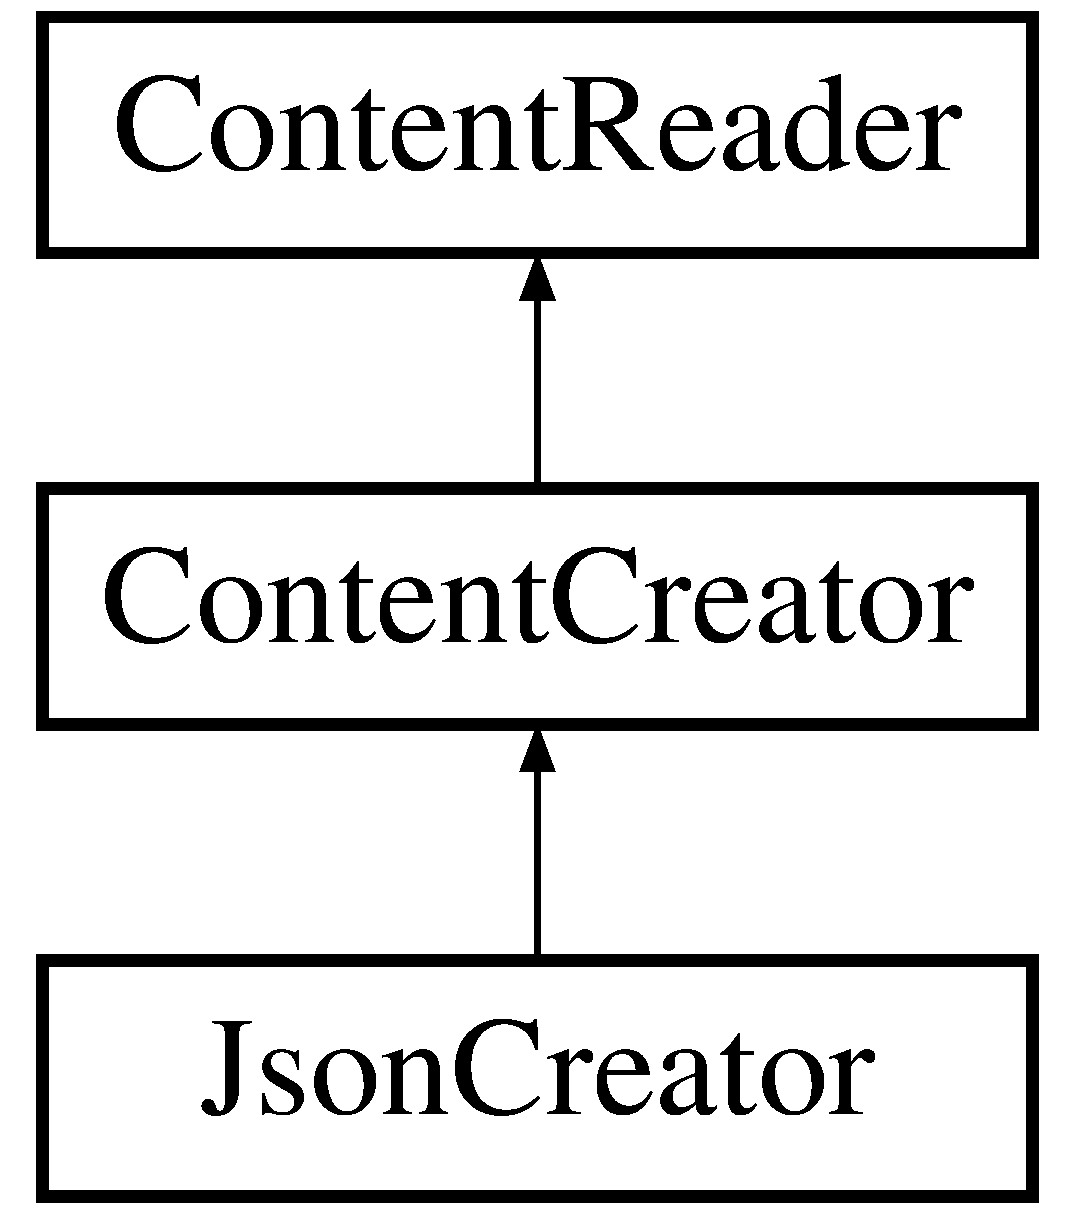
\includegraphics[height=3.000000cm]{classContentCreator}
\end{center}
\end{figure}
\subsection*{Public Member Functions}
\begin{DoxyCompactItemize}
\item 
virtual void \mbox{\hyperlink{classContentReader_a7fff2e63a2e8fa216665604f69974e1d}{parse}} (std\+::string \&text, \mbox{\hyperlink{classElement}{Element}} $\ast$$\ast$e) const =0
\item 
virtual void \mbox{\hyperlink{classContentReader_a7eef37b8b9761e21c0a3907ff94c72f7}{parse\+Content}} (std\+::string \&text, \mbox{\hyperlink{classElementInt}{Element\+Int}} $\ast$e) const =0
\item 
virtual void \mbox{\hyperlink{classContentReader_a310678ddc37a05aca2f13db73b22abe5}{parse\+Content}} (std\+::string \&text, \mbox{\hyperlink{classElementString}{Element\+String}} $\ast$e) const =0
\item 
virtual void \mbox{\hyperlink{classContentReader_a3ee0aec579c723f17742e10fe7c75e39}{parse\+Content}} (std\+::string \&text, \mbox{\hyperlink{classElementBoolean}{Element\+Boolean}} $\ast$e) const =0
\item 
virtual void \mbox{\hyperlink{classContentReader_a91fdd738983dcc7a246c3c163007dfa9}{parse\+Content}} (std\+::string \&text, \mbox{\hyperlink{classElementArray}{Element\+Array}} $\ast$e) const =0
\item 
virtual void \mbox{\hyperlink{classContentReader_a59a8de2bf3436e46b4d029a9b3c3c9da}{parse\+Content}} (std\+::string \&text, \mbox{\hyperlink{classElementObject}{Element\+Object}} $\ast$e) const =0
\item 
virtual void \mbox{\hyperlink{classContentReader_ab4ba739ee5241848ae8af86e64e43a40}{parse\+Content}} (std\+::string \&text, \mbox{\hyperlink{classElementDouble}{Element\+Double}} $\ast$e) const =0
\end{DoxyCompactItemize}


\subsection{Detailed Description}
An abstract creator. A creator is a particular reader that only works in the \mbox{\hyperlink{classElement}{Element}} to string way. \begin{DoxySeeAlso}{See also}
\mbox{\hyperlink{classContentReader}{Content\+Reader}} 

\mbox{\hyperlink{classElement}{Element}}
\end{DoxySeeAlso}
\begin{DoxyAuthor}{Author}
Mathieu Lochet 
\end{DoxyAuthor}
\begin{DoxyVersion}{Version}
1 
\end{DoxyVersion}


\subsection{Member Function Documentation}
\mbox{\Hypertarget{classContentReader_a7fff2e63a2e8fa216665604f69974e1d}\label{classContentReader_a7fff2e63a2e8fa216665604f69974e1d}} 
\index{Content\+Creator@{Content\+Creator}!parse@{parse}}
\index{parse@{parse}!Content\+Creator@{Content\+Creator}}
\subsubsection{\texorpdfstring{parse()}{parse()}}
{\footnotesize\ttfamily virtual void Content\+Reader\+::parse (\begin{DoxyParamCaption}\item[{std\+::string \&}]{text,  }\item[{\mbox{\hyperlink{classElement}{Element}} $\ast$$\ast$}]{e }\end{DoxyParamCaption}) const\hspace{0.3cm}{\ttfamily [pure virtual]}, {\ttfamily [inherited]}}

The entry point of the parser\+: it reads the text and generate the first element according to rules. Calls the corresponding methods for recursive parsing. (opposite works as well) \begin{DoxySeeAlso}{See also}
\mbox{\hyperlink{classContentReader_a7eef37b8b9761e21c0a3907ff94c72f7}{parse\+Content}} 

\mbox{\hyperlink{classElement}{Element}}
\end{DoxySeeAlso}

\begin{DoxyParams}{Parameters}
{\em text} & a given text \\
\hline
{\em e} & the root \mbox{\hyperlink{classElement}{Element}} that will be generated (or used) \\
\hline
\end{DoxyParams}


Implemented in \mbox{\hyperlink{classJsonCreator_a505ff309c6b144d29478804b0e187c6f}{Json\+Creator}}, and \mbox{\hyperlink{classJsonParser_a3ec3a9fcc8a63f987b4749d60b0568df}{Json\+Parser}}.

\mbox{\Hypertarget{classContentReader_a7eef37b8b9761e21c0a3907ff94c72f7}\label{classContentReader_a7eef37b8b9761e21c0a3907ff94c72f7}} 
\index{Content\+Creator@{Content\+Creator}!parse\+Content@{parse\+Content}}
\index{parse\+Content@{parse\+Content}!Content\+Creator@{Content\+Creator}}
\subsubsection{\texorpdfstring{parse\+Content()}{parseContent()}\hspace{0.1cm}{\footnotesize\ttfamily [1/6]}}
{\footnotesize\ttfamily virtual void Content\+Reader\+::parse\+Content (\begin{DoxyParamCaption}\item[{std\+::string \&}]{text,  }\item[{\mbox{\hyperlink{classElementInt}{Element\+Int}} $\ast$}]{e }\end{DoxyParamCaption}) const\hspace{0.3cm}{\ttfamily [pure virtual]}, {\ttfamily [inherited]}}

Generates an integer from a given string. Calls the method parse with the rest of the string. (opposite works as well) \begin{DoxySeeAlso}{See also}
\mbox{\hyperlink{classContentReader_a7fff2e63a2e8fa216665604f69974e1d}{parse}} 

\mbox{\hyperlink{classElementInt}{Element\+Int}}
\end{DoxySeeAlso}

\begin{DoxyParams}{Parameters}
{\em text} & a given text \\
\hline
{\em e} & the int \mbox{\hyperlink{classElement}{Element}} that will be generated (or used) \\
\hline
\end{DoxyParams}


Implemented in \mbox{\hyperlink{classJsonCreator_a0fe34794ee3563c3e0bc35006129fcdc}{Json\+Creator}}, and \mbox{\hyperlink{classJsonParser_ac80cf84ff2565f4c1f3a0f5ddb559c96}{Json\+Parser}}.

\mbox{\Hypertarget{classContentReader_a310678ddc37a05aca2f13db73b22abe5}\label{classContentReader_a310678ddc37a05aca2f13db73b22abe5}} 
\index{Content\+Creator@{Content\+Creator}!parse\+Content@{parse\+Content}}
\index{parse\+Content@{parse\+Content}!Content\+Creator@{Content\+Creator}}
\subsubsection{\texorpdfstring{parse\+Content()}{parseContent()}\hspace{0.1cm}{\footnotesize\ttfamily [2/6]}}
{\footnotesize\ttfamily virtual void Content\+Reader\+::parse\+Content (\begin{DoxyParamCaption}\item[{std\+::string \&}]{text,  }\item[{\mbox{\hyperlink{classElementString}{Element\+String}} $\ast$}]{e }\end{DoxyParamCaption}) const\hspace{0.3cm}{\ttfamily [pure virtual]}, {\ttfamily [inherited]}}

Generates an string from a given string. it stops with the defined rules of the parser. Calls the method parse with the rest of the string. (opposite works as well) \begin{DoxySeeAlso}{See also}
\mbox{\hyperlink{classContentReader_a7fff2e63a2e8fa216665604f69974e1d}{parse}} 

\mbox{\hyperlink{classElementString}{Element\+String}}
\end{DoxySeeAlso}

\begin{DoxyParams}{Parameters}
{\em text} & a given text \\
\hline
{\em e} & the string \mbox{\hyperlink{classElement}{Element}} that will be generated (or used) \\
\hline
\end{DoxyParams}


Implemented in \mbox{\hyperlink{classJsonCreator_acf8d7cd3dcbb669fd9eb5dec95e069f3}{Json\+Creator}}, and \mbox{\hyperlink{classJsonParser_a94737a7518f05e4ed43a753f4148b354}{Json\+Parser}}.

\mbox{\Hypertarget{classContentReader_a3ee0aec579c723f17742e10fe7c75e39}\label{classContentReader_a3ee0aec579c723f17742e10fe7c75e39}} 
\index{Content\+Creator@{Content\+Creator}!parse\+Content@{parse\+Content}}
\index{parse\+Content@{parse\+Content}!Content\+Creator@{Content\+Creator}}
\subsubsection{\texorpdfstring{parse\+Content()}{parseContent()}\hspace{0.1cm}{\footnotesize\ttfamily [3/6]}}
{\footnotesize\ttfamily virtual void Content\+Reader\+::parse\+Content (\begin{DoxyParamCaption}\item[{std\+::string \&}]{text,  }\item[{\mbox{\hyperlink{classElementBoolean}{Element\+Boolean}} $\ast$}]{e }\end{DoxyParamCaption}) const\hspace{0.3cm}{\ttfamily [pure virtual]}, {\ttfamily [inherited]}}

Generates an boolean from a given string. Calls the method parse with the rest of the string. (opposite works as well) \begin{DoxySeeAlso}{See also}
\mbox{\hyperlink{classContentReader_a7fff2e63a2e8fa216665604f69974e1d}{parse}} 

\mbox{\hyperlink{classElementBoolean}{Element\+Boolean}}
\end{DoxySeeAlso}

\begin{DoxyParams}{Parameters}
{\em text} & a given text \\
\hline
{\em e} & the boolean \mbox{\hyperlink{classElement}{Element}} that will be generated (or used) \\
\hline
\end{DoxyParams}


Implemented in \mbox{\hyperlink{classJsonCreator_a95fb65046a7467b8e48feaf92a62b40c}{Json\+Creator}}, and \mbox{\hyperlink{classJsonParser_a0857f5d286e5f0b973e2791e5e7a4e83}{Json\+Parser}}.

\mbox{\Hypertarget{classContentReader_a91fdd738983dcc7a246c3c163007dfa9}\label{classContentReader_a91fdd738983dcc7a246c3c163007dfa9}} 
\index{Content\+Creator@{Content\+Creator}!parse\+Content@{parse\+Content}}
\index{parse\+Content@{parse\+Content}!Content\+Creator@{Content\+Creator}}
\subsubsection{\texorpdfstring{parse\+Content()}{parseContent()}\hspace{0.1cm}{\footnotesize\ttfamily [4/6]}}
{\footnotesize\ttfamily virtual void Content\+Reader\+::parse\+Content (\begin{DoxyParamCaption}\item[{std\+::string \&}]{text,  }\item[{\mbox{\hyperlink{classElementArray}{Element\+Array}} $\ast$}]{e }\end{DoxyParamCaption}) const\hspace{0.3cm}{\ttfamily [pure virtual]}, {\ttfamily [inherited]}}

Generates an array of Elements from a given string. Calls the method parse with the rest of the string and parse each of the found elements of the array. (opposite works as well) \begin{DoxySeeAlso}{See also}
\mbox{\hyperlink{classContentReader_a7fff2e63a2e8fa216665604f69974e1d}{parse}} 

\mbox{\hyperlink{classElement}{Element}} 

\mbox{\hyperlink{classElementArray}{Element\+Array}}
\end{DoxySeeAlso}

\begin{DoxyParams}{Parameters}
{\em text} & a given text \\
\hline
{\em e} & the array \mbox{\hyperlink{classElement}{Element}} that will be generated (or used) \\
\hline
\end{DoxyParams}


Implemented in \mbox{\hyperlink{classJsonCreator_a694669d359eb73890a9e9f247c4ebab4}{Json\+Creator}}, and \mbox{\hyperlink{classJsonParser_aa728c443b247b83cdf6cedb406d8940d}{Json\+Parser}}.

\mbox{\Hypertarget{classContentReader_a59a8de2bf3436e46b4d029a9b3c3c9da}\label{classContentReader_a59a8de2bf3436e46b4d029a9b3c3c9da}} 
\index{Content\+Creator@{Content\+Creator}!parse\+Content@{parse\+Content}}
\index{parse\+Content@{parse\+Content}!Content\+Creator@{Content\+Creator}}
\subsubsection{\texorpdfstring{parse\+Content()}{parseContent()}\hspace{0.1cm}{\footnotesize\ttfamily [5/6]}}
{\footnotesize\ttfamily virtual void Content\+Reader\+::parse\+Content (\begin{DoxyParamCaption}\item[{std\+::string \&}]{text,  }\item[{\mbox{\hyperlink{classElementObject}{Element\+Object}} $\ast$}]{e }\end{DoxyParamCaption}) const\hspace{0.3cm}{\ttfamily [pure virtual]}, {\ttfamily [inherited]}}

Generates an object of $<$key (string), Elements$>$ from a given string. Calls the method parse with the rest of the string and parse each of the found elements of the object. (opposite works as well) \begin{DoxySeeAlso}{See also}
\mbox{\hyperlink{classContentReader_a7fff2e63a2e8fa216665604f69974e1d}{parse}} 

\mbox{\hyperlink{classElement}{Element}} 

\mbox{\hyperlink{classElementObject}{Element\+Object}}
\end{DoxySeeAlso}

\begin{DoxyParams}{Parameters}
{\em text} & a given text \\
\hline
{\em e} & the object \mbox{\hyperlink{classElement}{Element}} that will be generated (or used) \\
\hline
\end{DoxyParams}


Implemented in \mbox{\hyperlink{classJsonCreator_a9f57af1a7925074b8e3e4175f74c886a}{Json\+Creator}}, and \mbox{\hyperlink{classJsonParser_a7d4fad0f0947a74ca158dc1922c97355}{Json\+Parser}}.

\mbox{\Hypertarget{classContentReader_ab4ba739ee5241848ae8af86e64e43a40}\label{classContentReader_ab4ba739ee5241848ae8af86e64e43a40}} 
\index{Content\+Creator@{Content\+Creator}!parse\+Content@{parse\+Content}}
\index{parse\+Content@{parse\+Content}!Content\+Creator@{Content\+Creator}}
\subsubsection{\texorpdfstring{parse\+Content()}{parseContent()}\hspace{0.1cm}{\footnotesize\ttfamily [6/6]}}
{\footnotesize\ttfamily virtual void Content\+Reader\+::parse\+Content (\begin{DoxyParamCaption}\item[{std\+::string \&}]{text,  }\item[{\mbox{\hyperlink{classElementDouble}{Element\+Double}} $\ast$}]{e }\end{DoxyParamCaption}) const\hspace{0.3cm}{\ttfamily [pure virtual]}, {\ttfamily [inherited]}}

Generates an double from a given string. Calls the method parse with the rest of the string. (opposite works as well) \begin{DoxySeeAlso}{See also}
\mbox{\hyperlink{classContentReader_a7fff2e63a2e8fa216665604f69974e1d}{parse}} 

\mbox{\hyperlink{classElementDouble}{Element\+Double}}
\end{DoxySeeAlso}

\begin{DoxyParams}{Parameters}
{\em text} & a given text \\
\hline
{\em e} & the double \mbox{\hyperlink{classElement}{Element}} that will be generated (or used) \\
\hline
\end{DoxyParams}


Implemented in \mbox{\hyperlink{classJsonCreator_a5e841806165fd5cb595d9f7d7c924080}{Json\+Creator}}, and \mbox{\hyperlink{classJsonParser_a07a4f2b10547d5f2251bc1f7b09d02c1}{Json\+Parser}}.



The documentation for this class was generated from the following file\+:\begin{DoxyCompactItemize}
\item 
block\+\_\+chain/utils/serialization/Parser.\+h\end{DoxyCompactItemize}

\hypertarget{classContentParser}{}\section{Content\+Parser Class Reference}
\label{classContentParser}\index{Content\+Parser@{Content\+Parser}}


{\ttfamily \#include $<$Parser.\+h$>$}

Inheritance diagram for Content\+Parser\+:\begin{figure}[H]
\begin{center}
\leavevmode
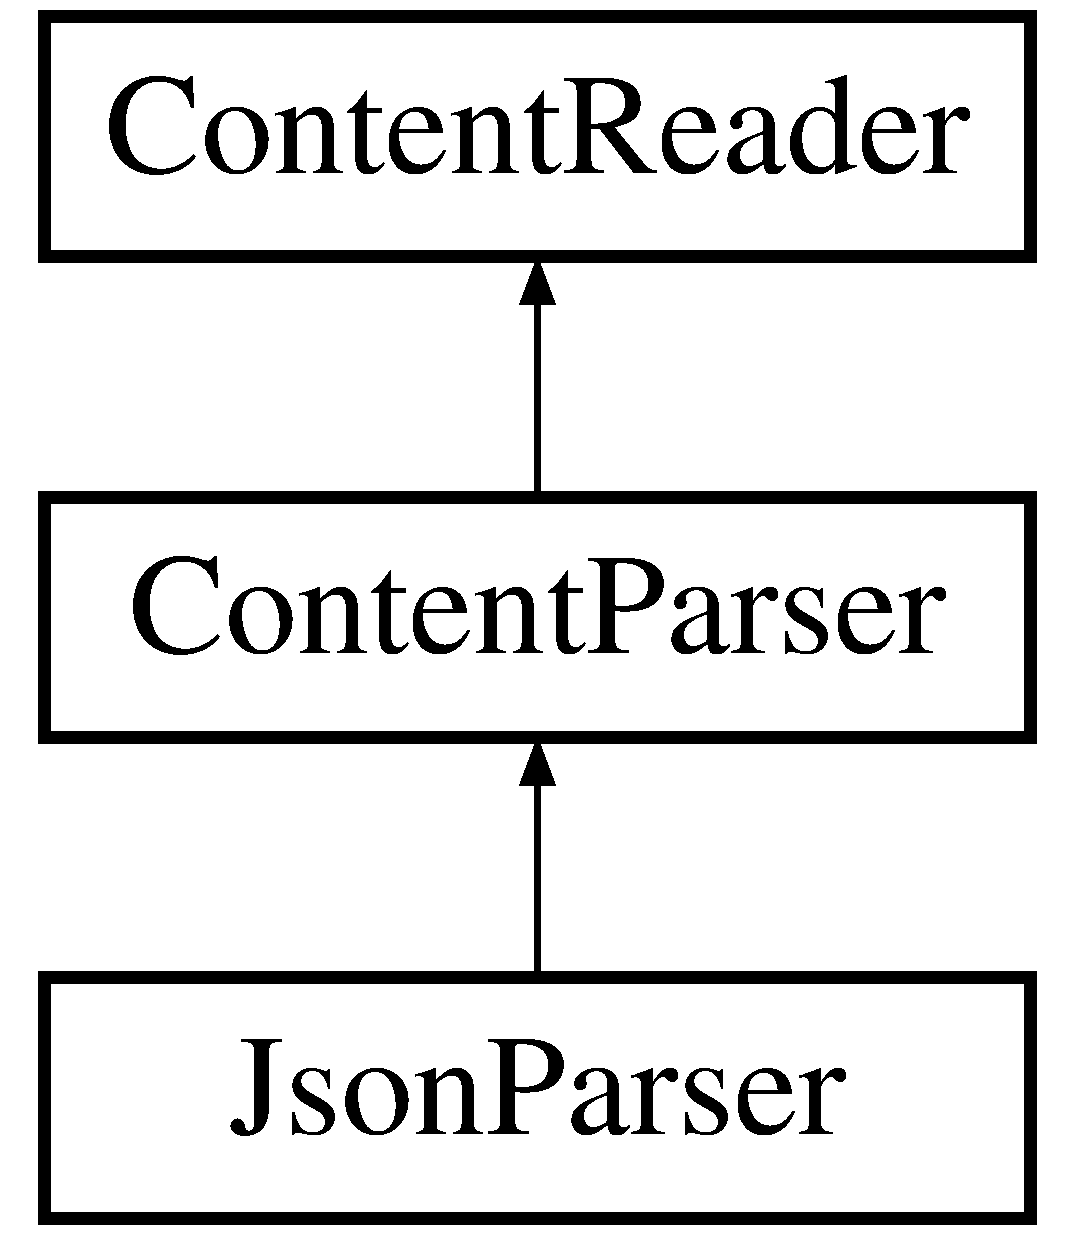
\includegraphics[height=3.000000cm]{classContentParser}
\end{center}
\end{figure}
\subsection*{Public Member Functions}
\begin{DoxyCompactItemize}
\item 
virtual void \mbox{\hyperlink{classContentReader_a7fff2e63a2e8fa216665604f69974e1d}{parse}} (std\+::string \&text, \mbox{\hyperlink{classElement}{Element}} $\ast$$\ast$e) const =0
\item 
virtual void \mbox{\hyperlink{classContentReader_a7eef37b8b9761e21c0a3907ff94c72f7}{parse\+Content}} (std\+::string \&text, \mbox{\hyperlink{classElementInt}{Element\+Int}} $\ast$e) const =0
\item 
virtual void \mbox{\hyperlink{classContentReader_a310678ddc37a05aca2f13db73b22abe5}{parse\+Content}} (std\+::string \&text, \mbox{\hyperlink{classElementString}{Element\+String}} $\ast$e) const =0
\item 
virtual void \mbox{\hyperlink{classContentReader_a3ee0aec579c723f17742e10fe7c75e39}{parse\+Content}} (std\+::string \&text, \mbox{\hyperlink{classElementBoolean}{Element\+Boolean}} $\ast$e) const =0
\item 
virtual void \mbox{\hyperlink{classContentReader_a91fdd738983dcc7a246c3c163007dfa9}{parse\+Content}} (std\+::string \&text, \mbox{\hyperlink{classElementArray}{Element\+Array}} $\ast$e) const =0
\item 
virtual void \mbox{\hyperlink{classContentReader_a59a8de2bf3436e46b4d029a9b3c3c9da}{parse\+Content}} (std\+::string \&text, \mbox{\hyperlink{classElementObject}{Element\+Object}} $\ast$e) const =0
\item 
virtual void \mbox{\hyperlink{classContentReader_ab4ba739ee5241848ae8af86e64e43a40}{parse\+Content}} (std\+::string \&text, \mbox{\hyperlink{classElementDouble}{Element\+Double}} $\ast$e) const =0
\item 
virtual const char $\ast$ \mbox{\hyperlink{classContentReader_a1495a4402c4fac02d8cd2542b61c6eed}{get\+\_\+encoding}} () const =0
\end{DoxyCompactItemize}


\subsection{Detailed Description}
An abstract parser. A parser is a particular reader that only works in the string to \mbox{\hyperlink{classElement}{Element}} way. \begin{DoxySeeAlso}{See also}
\mbox{\hyperlink{classContentReader}{Content\+Reader}} 

\mbox{\hyperlink{classElement}{Element}}
\end{DoxySeeAlso}
\begin{DoxyAuthor}{Author}
Mathieu Lochet 
\end{DoxyAuthor}
\begin{DoxyVersion}{Version}
1 
\end{DoxyVersion}


\subsection{Member Function Documentation}
\mbox{\Hypertarget{classContentReader_a1495a4402c4fac02d8cd2542b61c6eed}\label{classContentReader_a1495a4402c4fac02d8cd2542b61c6eed}} 
\index{Content\+Parser@{Content\+Parser}!get\+\_\+encoding@{get\+\_\+encoding}}
\index{get\+\_\+encoding@{get\+\_\+encoding}!Content\+Parser@{Content\+Parser}}
\subsubsection{\texorpdfstring{get\+\_\+encoding()}{get\_encoding()}}
{\footnotesize\ttfamily virtual const char$\ast$ Content\+Reader\+::get\+\_\+encoding (\begin{DoxyParamCaption}{ }\end{DoxyParamCaption}) const\hspace{0.3cm}{\ttfamily [pure virtual]}, {\ttfamily [inherited]}}

Get the encoding corresponding to the reader

\begin{DoxyReturn}{Returns}
The corresponding encoding for serialization 
\end{DoxyReturn}


Implemented in \mbox{\hyperlink{classJsonCreator_ab7313de0040d40a26a9386eb3714120c}{Json\+Creator}}, and \mbox{\hyperlink{classJsonParser_a449d410175c5055eb171f00105305ec5}{Json\+Parser}}.

\mbox{\Hypertarget{classContentReader_a7fff2e63a2e8fa216665604f69974e1d}\label{classContentReader_a7fff2e63a2e8fa216665604f69974e1d}} 
\index{Content\+Parser@{Content\+Parser}!parse@{parse}}
\index{parse@{parse}!Content\+Parser@{Content\+Parser}}
\subsubsection{\texorpdfstring{parse()}{parse()}}
{\footnotesize\ttfamily virtual void Content\+Reader\+::parse (\begin{DoxyParamCaption}\item[{std\+::string \&}]{text,  }\item[{\mbox{\hyperlink{classElement}{Element}} $\ast$$\ast$}]{e }\end{DoxyParamCaption}) const\hspace{0.3cm}{\ttfamily [pure virtual]}, {\ttfamily [inherited]}}

The entry point of the parser\+: it reads the text and generates the first element according to rules. Calls the corresponding methods for recursive parsing. (opposite works as well) \begin{DoxySeeAlso}{See also}
\mbox{\hyperlink{classContentReader_a7eef37b8b9761e21c0a3907ff94c72f7}{parse\+Content}} 

\mbox{\hyperlink{classElement}{Element}}
\end{DoxySeeAlso}

\begin{DoxyParams}{Parameters}
{\em text} & a given text \\
\hline
{\em e} & the root \mbox{\hyperlink{classElement}{Element}} that will be generated (or used) \\
\hline
\end{DoxyParams}


Implemented in \mbox{\hyperlink{classJsonCreator_a505ff309c6b144d29478804b0e187c6f}{Json\+Creator}}, and \mbox{\hyperlink{classJsonParser_a3ec3a9fcc8a63f987b4749d60b0568df}{Json\+Parser}}.

\mbox{\Hypertarget{classContentReader_a7eef37b8b9761e21c0a3907ff94c72f7}\label{classContentReader_a7eef37b8b9761e21c0a3907ff94c72f7}} 
\index{Content\+Parser@{Content\+Parser}!parse\+Content@{parse\+Content}}
\index{parse\+Content@{parse\+Content}!Content\+Parser@{Content\+Parser}}
\subsubsection{\texorpdfstring{parse\+Content()}{parseContent()}\hspace{0.1cm}{\footnotesize\ttfamily [1/6]}}
{\footnotesize\ttfamily virtual void Content\+Reader\+::parse\+Content (\begin{DoxyParamCaption}\item[{std\+::string \&}]{text,  }\item[{\mbox{\hyperlink{classElementInt}{Element\+Int}} $\ast$}]{e }\end{DoxyParamCaption}) const\hspace{0.3cm}{\ttfamily [pure virtual]}, {\ttfamily [inherited]}}

Generates an integer from a given string. Calls the method parse with the rest of the string. (opposite works as well) \begin{DoxySeeAlso}{See also}
\mbox{\hyperlink{classContentReader_a7fff2e63a2e8fa216665604f69974e1d}{parse}} 

\mbox{\hyperlink{classElementInt}{Element\+Int}}
\end{DoxySeeAlso}

\begin{DoxyParams}{Parameters}
{\em text} & a given text \\
\hline
{\em e} & the int \mbox{\hyperlink{classElement}{Element}} that will be generated (or used) \\
\hline
\end{DoxyParams}


Implemented in \mbox{\hyperlink{classJsonCreator_a0fe34794ee3563c3e0bc35006129fcdc}{Json\+Creator}}, and \mbox{\hyperlink{classJsonParser_ac80cf84ff2565f4c1f3a0f5ddb559c96}{Json\+Parser}}.

\mbox{\Hypertarget{classContentReader_a310678ddc37a05aca2f13db73b22abe5}\label{classContentReader_a310678ddc37a05aca2f13db73b22abe5}} 
\index{Content\+Parser@{Content\+Parser}!parse\+Content@{parse\+Content}}
\index{parse\+Content@{parse\+Content}!Content\+Parser@{Content\+Parser}}
\subsubsection{\texorpdfstring{parse\+Content()}{parseContent()}\hspace{0.1cm}{\footnotesize\ttfamily [2/6]}}
{\footnotesize\ttfamily virtual void Content\+Reader\+::parse\+Content (\begin{DoxyParamCaption}\item[{std\+::string \&}]{text,  }\item[{\mbox{\hyperlink{classElementString}{Element\+String}} $\ast$}]{e }\end{DoxyParamCaption}) const\hspace{0.3cm}{\ttfamily [pure virtual]}, {\ttfamily [inherited]}}

Generates an string from a given string. it stops with the defined rules of the parser. Calls the method parse with the rest of the string. (opposite works as well) \begin{DoxySeeAlso}{See also}
\mbox{\hyperlink{classContentReader_a7fff2e63a2e8fa216665604f69974e1d}{parse}} 

\mbox{\hyperlink{classElementString}{Element\+String}}
\end{DoxySeeAlso}

\begin{DoxyParams}{Parameters}
{\em text} & a given text \\
\hline
{\em e} & the string \mbox{\hyperlink{classElement}{Element}} that will be generated (or used) \\
\hline
\end{DoxyParams}


Implemented in \mbox{\hyperlink{classJsonCreator_acf8d7cd3dcbb669fd9eb5dec95e069f3}{Json\+Creator}}, and \mbox{\hyperlink{classJsonParser_a94737a7518f05e4ed43a753f4148b354}{Json\+Parser}}.

\mbox{\Hypertarget{classContentReader_a3ee0aec579c723f17742e10fe7c75e39}\label{classContentReader_a3ee0aec579c723f17742e10fe7c75e39}} 
\index{Content\+Parser@{Content\+Parser}!parse\+Content@{parse\+Content}}
\index{parse\+Content@{parse\+Content}!Content\+Parser@{Content\+Parser}}
\subsubsection{\texorpdfstring{parse\+Content()}{parseContent()}\hspace{0.1cm}{\footnotesize\ttfamily [3/6]}}
{\footnotesize\ttfamily virtual void Content\+Reader\+::parse\+Content (\begin{DoxyParamCaption}\item[{std\+::string \&}]{text,  }\item[{\mbox{\hyperlink{classElementBoolean}{Element\+Boolean}} $\ast$}]{e }\end{DoxyParamCaption}) const\hspace{0.3cm}{\ttfamily [pure virtual]}, {\ttfamily [inherited]}}

Generates an boolean from a given string. Calls the method parse with the rest of the string. (opposite works as well) \begin{DoxySeeAlso}{See also}
\mbox{\hyperlink{classContentReader_a7fff2e63a2e8fa216665604f69974e1d}{parse}} 

\mbox{\hyperlink{classElementBoolean}{Element\+Boolean}}
\end{DoxySeeAlso}

\begin{DoxyParams}{Parameters}
{\em text} & a given text \\
\hline
{\em e} & the boolean \mbox{\hyperlink{classElement}{Element}} that will be generated (or used) \\
\hline
\end{DoxyParams}


Implemented in \mbox{\hyperlink{classJsonCreator_a95fb65046a7467b8e48feaf92a62b40c}{Json\+Creator}}, and \mbox{\hyperlink{classJsonParser_a0857f5d286e5f0b973e2791e5e7a4e83}{Json\+Parser}}.

\mbox{\Hypertarget{classContentReader_a91fdd738983dcc7a246c3c163007dfa9}\label{classContentReader_a91fdd738983dcc7a246c3c163007dfa9}} 
\index{Content\+Parser@{Content\+Parser}!parse\+Content@{parse\+Content}}
\index{parse\+Content@{parse\+Content}!Content\+Parser@{Content\+Parser}}
\subsubsection{\texorpdfstring{parse\+Content()}{parseContent()}\hspace{0.1cm}{\footnotesize\ttfamily [4/6]}}
{\footnotesize\ttfamily virtual void Content\+Reader\+::parse\+Content (\begin{DoxyParamCaption}\item[{std\+::string \&}]{text,  }\item[{\mbox{\hyperlink{classElementArray}{Element\+Array}} $\ast$}]{e }\end{DoxyParamCaption}) const\hspace{0.3cm}{\ttfamily [pure virtual]}, {\ttfamily [inherited]}}

Generates an array of Elements from a given string. Calls the method parse with the rest of the string and parse each of the found elements of the array. (opposite works as well) \begin{DoxySeeAlso}{See also}
\mbox{\hyperlink{classContentReader_a7fff2e63a2e8fa216665604f69974e1d}{parse}} 

\mbox{\hyperlink{classElement}{Element}} 

\mbox{\hyperlink{classElementArray}{Element\+Array}}
\end{DoxySeeAlso}

\begin{DoxyParams}{Parameters}
{\em text} & a given text \\
\hline
{\em e} & the array \mbox{\hyperlink{classElement}{Element}} that will be generated (or used) \\
\hline
\end{DoxyParams}


Implemented in \mbox{\hyperlink{classJsonCreator_a694669d359eb73890a9e9f247c4ebab4}{Json\+Creator}}, and \mbox{\hyperlink{classJsonParser_aa728c443b247b83cdf6cedb406d8940d}{Json\+Parser}}.

\mbox{\Hypertarget{classContentReader_a59a8de2bf3436e46b4d029a9b3c3c9da}\label{classContentReader_a59a8de2bf3436e46b4d029a9b3c3c9da}} 
\index{Content\+Parser@{Content\+Parser}!parse\+Content@{parse\+Content}}
\index{parse\+Content@{parse\+Content}!Content\+Parser@{Content\+Parser}}
\subsubsection{\texorpdfstring{parse\+Content()}{parseContent()}\hspace{0.1cm}{\footnotesize\ttfamily [5/6]}}
{\footnotesize\ttfamily virtual void Content\+Reader\+::parse\+Content (\begin{DoxyParamCaption}\item[{std\+::string \&}]{text,  }\item[{\mbox{\hyperlink{classElementObject}{Element\+Object}} $\ast$}]{e }\end{DoxyParamCaption}) const\hspace{0.3cm}{\ttfamily [pure virtual]}, {\ttfamily [inherited]}}

Generates an object of $<$key (string), Elements$>$ from a given string. Calls the method parse with the rest of the string and parse each of the found elements of the object. (opposite works as well) \begin{DoxySeeAlso}{See also}
\mbox{\hyperlink{classContentReader_a7fff2e63a2e8fa216665604f69974e1d}{parse}} 

\mbox{\hyperlink{classElement}{Element}} 

\mbox{\hyperlink{classElementObject}{Element\+Object}}
\end{DoxySeeAlso}

\begin{DoxyParams}{Parameters}
{\em text} & a given text \\
\hline
{\em e} & the object \mbox{\hyperlink{classElement}{Element}} that will be generated (or used) \\
\hline
\end{DoxyParams}


Implemented in \mbox{\hyperlink{classJsonCreator_a9f57af1a7925074b8e3e4175f74c886a}{Json\+Creator}}, and \mbox{\hyperlink{classJsonParser_a7d4fad0f0947a74ca158dc1922c97355}{Json\+Parser}}.

\mbox{\Hypertarget{classContentReader_ab4ba739ee5241848ae8af86e64e43a40}\label{classContentReader_ab4ba739ee5241848ae8af86e64e43a40}} 
\index{Content\+Parser@{Content\+Parser}!parse\+Content@{parse\+Content}}
\index{parse\+Content@{parse\+Content}!Content\+Parser@{Content\+Parser}}
\subsubsection{\texorpdfstring{parse\+Content()}{parseContent()}\hspace{0.1cm}{\footnotesize\ttfamily [6/6]}}
{\footnotesize\ttfamily virtual void Content\+Reader\+::parse\+Content (\begin{DoxyParamCaption}\item[{std\+::string \&}]{text,  }\item[{\mbox{\hyperlink{classElementDouble}{Element\+Double}} $\ast$}]{e }\end{DoxyParamCaption}) const\hspace{0.3cm}{\ttfamily [pure virtual]}, {\ttfamily [inherited]}}

Generates an double from a given string. Calls the method parse with the rest of the string. (opposite works as well) \begin{DoxySeeAlso}{See also}
\mbox{\hyperlink{classContentReader_a7fff2e63a2e8fa216665604f69974e1d}{parse}} 

\mbox{\hyperlink{classElementDouble}{Element\+Double}}
\end{DoxySeeAlso}

\begin{DoxyParams}{Parameters}
{\em text} & a given text \\
\hline
{\em e} & the double \mbox{\hyperlink{classElement}{Element}} that will be generated (or used) \\
\hline
\end{DoxyParams}


Implemented in \mbox{\hyperlink{classJsonCreator_a5e841806165fd5cb595d9f7d7c924080}{Json\+Creator}}, and \mbox{\hyperlink{classJsonParser_a07a4f2b10547d5f2251bc1f7b09d02c1}{Json\+Parser}}.



The documentation for this class was generated from the following file\+:\begin{DoxyCompactItemize}
\item 
block\+\_\+chain/utils/serialization/Parser.\+h\end{DoxyCompactItemize}

\hypertarget{classContentReader}{}\section{Content\+Reader Class Reference}
\label{classContentReader}\index{Content\+Reader@{Content\+Reader}}


{\ttfamily \#include $<$Parser.\+h$>$}

Inheritance diagram for Content\+Reader\+:\begin{figure}[H]
\begin{center}
\leavevmode
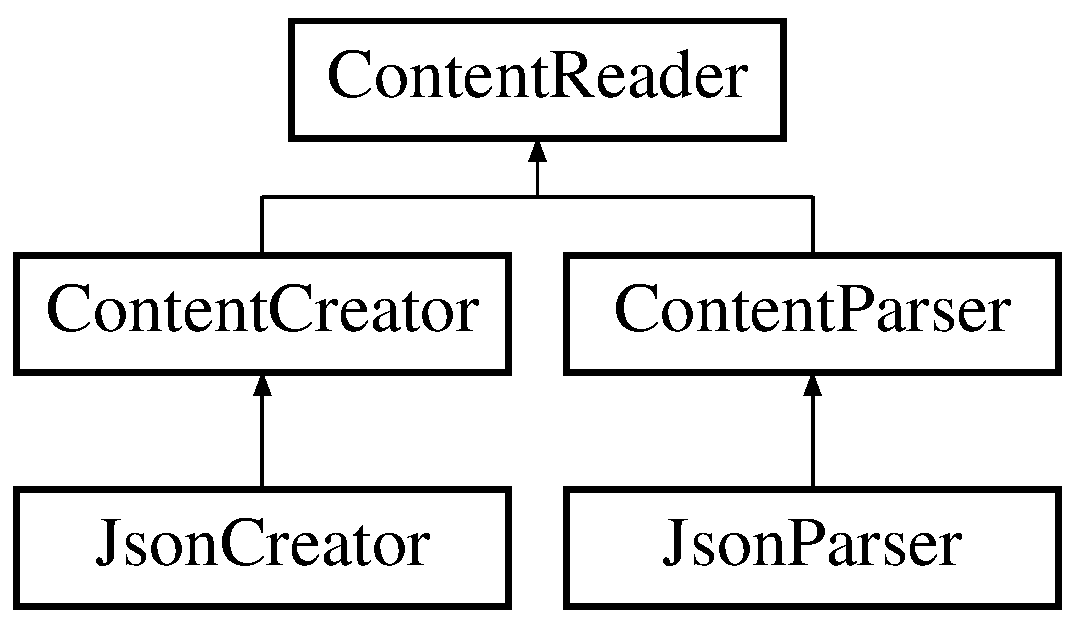
\includegraphics[height=3.000000cm]{classContentReader}
\end{center}
\end{figure}
\subsection*{Public Member Functions}
\begin{DoxyCompactItemize}
\item 
virtual void \mbox{\hyperlink{classContentReader_a7fff2e63a2e8fa216665604f69974e1d}{parse}} (std\+::string \&text, \mbox{\hyperlink{classElement}{Element}} $\ast$$\ast$e) const =0
\item 
virtual void \mbox{\hyperlink{classContentReader_a7eef37b8b9761e21c0a3907ff94c72f7}{parse\+Content}} (std\+::string \&text, \mbox{\hyperlink{classElementInt}{Element\+Int}} $\ast$e) const =0
\item 
virtual void \mbox{\hyperlink{classContentReader_a310678ddc37a05aca2f13db73b22abe5}{parse\+Content}} (std\+::string \&text, \mbox{\hyperlink{classElementString}{Element\+String}} $\ast$e) const =0
\item 
virtual void \mbox{\hyperlink{classContentReader_a3ee0aec579c723f17742e10fe7c75e39}{parse\+Content}} (std\+::string \&text, \mbox{\hyperlink{classElementBoolean}{Element\+Boolean}} $\ast$e) const =0
\item 
virtual void \mbox{\hyperlink{classContentReader_a91fdd738983dcc7a246c3c163007dfa9}{parse\+Content}} (std\+::string \&text, \mbox{\hyperlink{classElementArray}{Element\+Array}} $\ast$e) const =0
\item 
virtual void \mbox{\hyperlink{classContentReader_a59a8de2bf3436e46b4d029a9b3c3c9da}{parse\+Content}} (std\+::string \&text, \mbox{\hyperlink{classElementObject}{Element\+Object}} $\ast$e) const =0
\item 
virtual void \mbox{\hyperlink{classContentReader_ab4ba739ee5241848ae8af86e64e43a40}{parse\+Content}} (std\+::string \&text, \mbox{\hyperlink{classElementDouble}{Element\+Double}} $\ast$e) const =0
\end{DoxyCompactItemize}


\subsection{Detailed Description}
An abstract reader. A reader is a class that generates Elements with a given string. It work in the opposite way as well \begin{DoxySeeAlso}{See also}
\mbox{\hyperlink{classElement}{Element}}
\end{DoxySeeAlso}
\begin{DoxyAuthor}{Author}
Mathieu Lochet 
\end{DoxyAuthor}
\begin{DoxyVersion}{Version}
1 
\end{DoxyVersion}


\subsection{Member Function Documentation}
\mbox{\Hypertarget{classContentReader_a7fff2e63a2e8fa216665604f69974e1d}\label{classContentReader_a7fff2e63a2e8fa216665604f69974e1d}} 
\index{Content\+Reader@{Content\+Reader}!parse@{parse}}
\index{parse@{parse}!Content\+Reader@{Content\+Reader}}
\subsubsection{\texorpdfstring{parse()}{parse()}}
{\footnotesize\ttfamily virtual void Content\+Reader\+::parse (\begin{DoxyParamCaption}\item[{std\+::string \&}]{text,  }\item[{\mbox{\hyperlink{classElement}{Element}} $\ast$$\ast$}]{e }\end{DoxyParamCaption}) const\hspace{0.3cm}{\ttfamily [pure virtual]}}

The entry point of the parser\+: it reads the text and generate the first element according to rules. Calls the corresponding methods for recursive parsing. (opposite works as well) \begin{DoxySeeAlso}{See also}
\mbox{\hyperlink{classContentReader_a7eef37b8b9761e21c0a3907ff94c72f7}{parse\+Content}} 

\mbox{\hyperlink{classElement}{Element}}
\end{DoxySeeAlso}

\begin{DoxyParams}{Parameters}
{\em text} & a given text \\
\hline
{\em e} & the root \mbox{\hyperlink{classElement}{Element}} that will be generated (or used) \\
\hline
\end{DoxyParams}


Implemented in \mbox{\hyperlink{classJsonCreator_a505ff309c6b144d29478804b0e187c6f}{Json\+Creator}}, and \mbox{\hyperlink{classJsonParser_a3ec3a9fcc8a63f987b4749d60b0568df}{Json\+Parser}}.

\mbox{\Hypertarget{classContentReader_a7eef37b8b9761e21c0a3907ff94c72f7}\label{classContentReader_a7eef37b8b9761e21c0a3907ff94c72f7}} 
\index{Content\+Reader@{Content\+Reader}!parse\+Content@{parse\+Content}}
\index{parse\+Content@{parse\+Content}!Content\+Reader@{Content\+Reader}}
\subsubsection{\texorpdfstring{parse\+Content()}{parseContent()}\hspace{0.1cm}{\footnotesize\ttfamily [1/6]}}
{\footnotesize\ttfamily virtual void Content\+Reader\+::parse\+Content (\begin{DoxyParamCaption}\item[{std\+::string \&}]{text,  }\item[{\mbox{\hyperlink{classElementInt}{Element\+Int}} $\ast$}]{e }\end{DoxyParamCaption}) const\hspace{0.3cm}{\ttfamily [pure virtual]}}

Generates an integer from a given string. Calls the method parse with the rest of the string. (opposite works as well) \begin{DoxySeeAlso}{See also}
\mbox{\hyperlink{classContentReader_a7fff2e63a2e8fa216665604f69974e1d}{parse}} 

\mbox{\hyperlink{classElementInt}{Element\+Int}}
\end{DoxySeeAlso}

\begin{DoxyParams}{Parameters}
{\em text} & a given text \\
\hline
{\em e} & the int \mbox{\hyperlink{classElement}{Element}} that will be generated (or used) \\
\hline
\end{DoxyParams}


Implemented in \mbox{\hyperlink{classJsonCreator_a0fe34794ee3563c3e0bc35006129fcdc}{Json\+Creator}}, and \mbox{\hyperlink{classJsonParser_ac80cf84ff2565f4c1f3a0f5ddb559c96}{Json\+Parser}}.

\mbox{\Hypertarget{classContentReader_a310678ddc37a05aca2f13db73b22abe5}\label{classContentReader_a310678ddc37a05aca2f13db73b22abe5}} 
\index{Content\+Reader@{Content\+Reader}!parse\+Content@{parse\+Content}}
\index{parse\+Content@{parse\+Content}!Content\+Reader@{Content\+Reader}}
\subsubsection{\texorpdfstring{parse\+Content()}{parseContent()}\hspace{0.1cm}{\footnotesize\ttfamily [2/6]}}
{\footnotesize\ttfamily virtual void Content\+Reader\+::parse\+Content (\begin{DoxyParamCaption}\item[{std\+::string \&}]{text,  }\item[{\mbox{\hyperlink{classElementString}{Element\+String}} $\ast$}]{e }\end{DoxyParamCaption}) const\hspace{0.3cm}{\ttfamily [pure virtual]}}

Generates an string from a given string. it stops with the defined rules of the parser. Calls the method parse with the rest of the string. (opposite works as well) \begin{DoxySeeAlso}{See also}
\mbox{\hyperlink{classContentReader_a7fff2e63a2e8fa216665604f69974e1d}{parse}} 

\mbox{\hyperlink{classElementString}{Element\+String}}
\end{DoxySeeAlso}

\begin{DoxyParams}{Parameters}
{\em text} & a given text \\
\hline
{\em e} & the string \mbox{\hyperlink{classElement}{Element}} that will be generated (or used) \\
\hline
\end{DoxyParams}


Implemented in \mbox{\hyperlink{classJsonCreator_acf8d7cd3dcbb669fd9eb5dec95e069f3}{Json\+Creator}}, and \mbox{\hyperlink{classJsonParser_a94737a7518f05e4ed43a753f4148b354}{Json\+Parser}}.

\mbox{\Hypertarget{classContentReader_a3ee0aec579c723f17742e10fe7c75e39}\label{classContentReader_a3ee0aec579c723f17742e10fe7c75e39}} 
\index{Content\+Reader@{Content\+Reader}!parse\+Content@{parse\+Content}}
\index{parse\+Content@{parse\+Content}!Content\+Reader@{Content\+Reader}}
\subsubsection{\texorpdfstring{parse\+Content()}{parseContent()}\hspace{0.1cm}{\footnotesize\ttfamily [3/6]}}
{\footnotesize\ttfamily virtual void Content\+Reader\+::parse\+Content (\begin{DoxyParamCaption}\item[{std\+::string \&}]{text,  }\item[{\mbox{\hyperlink{classElementBoolean}{Element\+Boolean}} $\ast$}]{e }\end{DoxyParamCaption}) const\hspace{0.3cm}{\ttfamily [pure virtual]}}

Generates an boolean from a given string. Calls the method parse with the rest of the string. (opposite works as well) \begin{DoxySeeAlso}{See also}
\mbox{\hyperlink{classContentReader_a7fff2e63a2e8fa216665604f69974e1d}{parse}} 

\mbox{\hyperlink{classElementBoolean}{Element\+Boolean}}
\end{DoxySeeAlso}

\begin{DoxyParams}{Parameters}
{\em text} & a given text \\
\hline
{\em e} & the boolean \mbox{\hyperlink{classElement}{Element}} that will be generated (or used) \\
\hline
\end{DoxyParams}


Implemented in \mbox{\hyperlink{classJsonCreator_a95fb65046a7467b8e48feaf92a62b40c}{Json\+Creator}}, and \mbox{\hyperlink{classJsonParser_a0857f5d286e5f0b973e2791e5e7a4e83}{Json\+Parser}}.

\mbox{\Hypertarget{classContentReader_a91fdd738983dcc7a246c3c163007dfa9}\label{classContentReader_a91fdd738983dcc7a246c3c163007dfa9}} 
\index{Content\+Reader@{Content\+Reader}!parse\+Content@{parse\+Content}}
\index{parse\+Content@{parse\+Content}!Content\+Reader@{Content\+Reader}}
\subsubsection{\texorpdfstring{parse\+Content()}{parseContent()}\hspace{0.1cm}{\footnotesize\ttfamily [4/6]}}
{\footnotesize\ttfamily virtual void Content\+Reader\+::parse\+Content (\begin{DoxyParamCaption}\item[{std\+::string \&}]{text,  }\item[{\mbox{\hyperlink{classElementArray}{Element\+Array}} $\ast$}]{e }\end{DoxyParamCaption}) const\hspace{0.3cm}{\ttfamily [pure virtual]}}

Generates an array of Elements from a given string. Calls the method parse with the rest of the string and parse each of the found elements of the array. (opposite works as well) \begin{DoxySeeAlso}{See also}
\mbox{\hyperlink{classContentReader_a7fff2e63a2e8fa216665604f69974e1d}{parse}} 

\mbox{\hyperlink{classElement}{Element}} 

\mbox{\hyperlink{classElementArray}{Element\+Array}}
\end{DoxySeeAlso}

\begin{DoxyParams}{Parameters}
{\em text} & a given text \\
\hline
{\em e} & the array \mbox{\hyperlink{classElement}{Element}} that will be generated (or used) \\
\hline
\end{DoxyParams}


Implemented in \mbox{\hyperlink{classJsonCreator_a694669d359eb73890a9e9f247c4ebab4}{Json\+Creator}}, and \mbox{\hyperlink{classJsonParser_aa728c443b247b83cdf6cedb406d8940d}{Json\+Parser}}.

\mbox{\Hypertarget{classContentReader_a59a8de2bf3436e46b4d029a9b3c3c9da}\label{classContentReader_a59a8de2bf3436e46b4d029a9b3c3c9da}} 
\index{Content\+Reader@{Content\+Reader}!parse\+Content@{parse\+Content}}
\index{parse\+Content@{parse\+Content}!Content\+Reader@{Content\+Reader}}
\subsubsection{\texorpdfstring{parse\+Content()}{parseContent()}\hspace{0.1cm}{\footnotesize\ttfamily [5/6]}}
{\footnotesize\ttfamily virtual void Content\+Reader\+::parse\+Content (\begin{DoxyParamCaption}\item[{std\+::string \&}]{text,  }\item[{\mbox{\hyperlink{classElementObject}{Element\+Object}} $\ast$}]{e }\end{DoxyParamCaption}) const\hspace{0.3cm}{\ttfamily [pure virtual]}}

Generates an object of $<$key (string), Elements$>$ from a given string. Calls the method parse with the rest of the string and parse each of the found elements of the object. (opposite works as well) \begin{DoxySeeAlso}{See also}
\mbox{\hyperlink{classContentReader_a7fff2e63a2e8fa216665604f69974e1d}{parse}} 

\mbox{\hyperlink{classElement}{Element}} 

\mbox{\hyperlink{classElementObject}{Element\+Object}}
\end{DoxySeeAlso}

\begin{DoxyParams}{Parameters}
{\em text} & a given text \\
\hline
{\em e} & the object \mbox{\hyperlink{classElement}{Element}} that will be generated (or used) \\
\hline
\end{DoxyParams}


Implemented in \mbox{\hyperlink{classJsonCreator_a9f57af1a7925074b8e3e4175f74c886a}{Json\+Creator}}, and \mbox{\hyperlink{classJsonParser_a7d4fad0f0947a74ca158dc1922c97355}{Json\+Parser}}.

\mbox{\Hypertarget{classContentReader_ab4ba739ee5241848ae8af86e64e43a40}\label{classContentReader_ab4ba739ee5241848ae8af86e64e43a40}} 
\index{Content\+Reader@{Content\+Reader}!parse\+Content@{parse\+Content}}
\index{parse\+Content@{parse\+Content}!Content\+Reader@{Content\+Reader}}
\subsubsection{\texorpdfstring{parse\+Content()}{parseContent()}\hspace{0.1cm}{\footnotesize\ttfamily [6/6]}}
{\footnotesize\ttfamily virtual void Content\+Reader\+::parse\+Content (\begin{DoxyParamCaption}\item[{std\+::string \&}]{text,  }\item[{\mbox{\hyperlink{classElementDouble}{Element\+Double}} $\ast$}]{e }\end{DoxyParamCaption}) const\hspace{0.3cm}{\ttfamily [pure virtual]}}

Generates an double from a given string. Calls the method parse with the rest of the string. (opposite works as well) \begin{DoxySeeAlso}{See also}
\mbox{\hyperlink{classContentReader_a7fff2e63a2e8fa216665604f69974e1d}{parse}} 

\mbox{\hyperlink{classElementDouble}{Element\+Double}}
\end{DoxySeeAlso}

\begin{DoxyParams}{Parameters}
{\em text} & a given text \\
\hline
{\em e} & the double \mbox{\hyperlink{classElement}{Element}} that will be generated (or used) \\
\hline
\end{DoxyParams}


Implemented in \mbox{\hyperlink{classJsonCreator_a5e841806165fd5cb595d9f7d7c924080}{Json\+Creator}}, and \mbox{\hyperlink{classJsonParser_a07a4f2b10547d5f2251bc1f7b09d02c1}{Json\+Parser}}.



The documentation for this class was generated from the following file\+:\begin{DoxyCompactItemize}
\item 
block\+\_\+chain/utils/serialization/Parser.\+h\end{DoxyCompactItemize}

\hypertarget{classCustomRow}{}\section{Custom\+Row Class Reference}
\label{classCustomRow}\index{Custom\+Row@{Custom\+Row}}
Inheritance diagram for Custom\+Row\+:\begin{figure}[H]
\begin{center}
\leavevmode
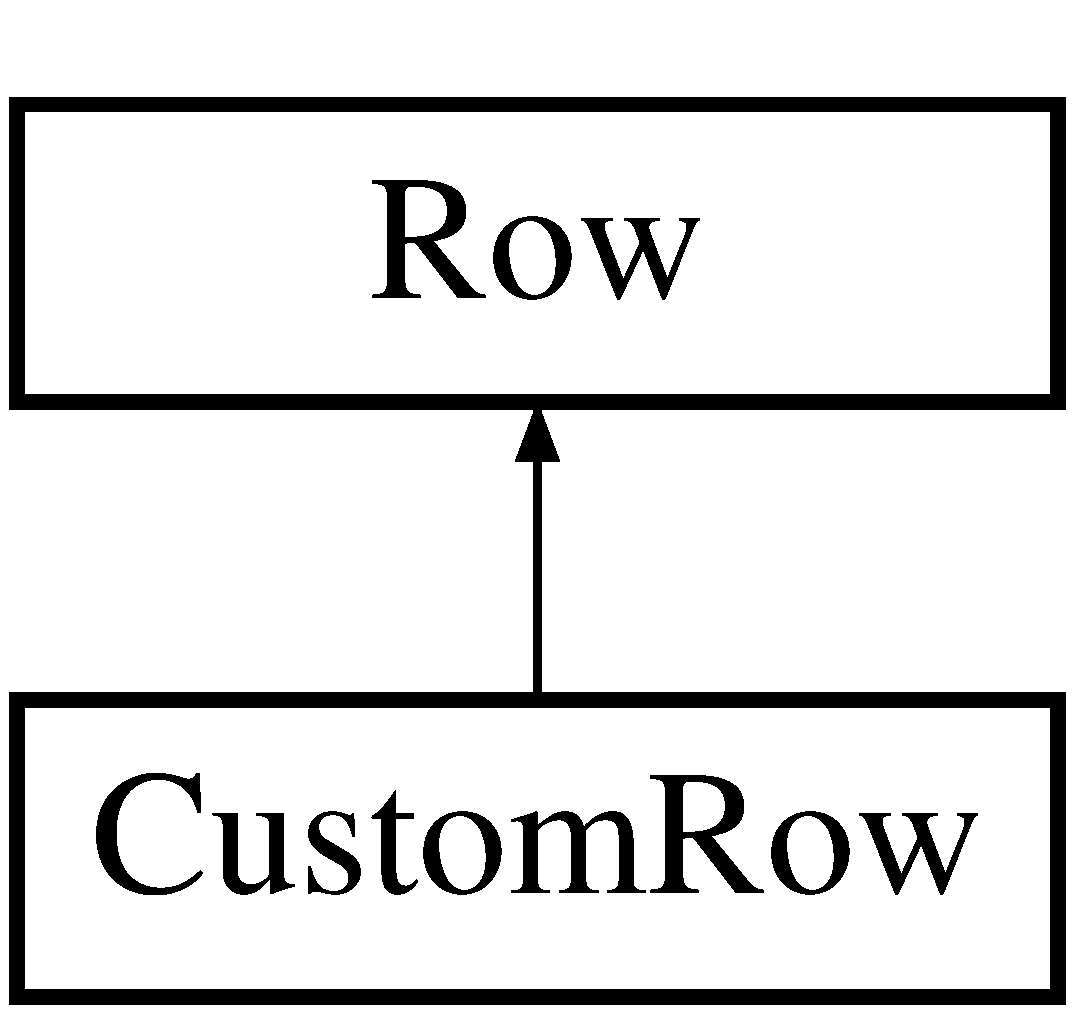
\includegraphics[height=2.000000cm]{classCustomRow}
\end{center}
\end{figure}
\subsection*{Public Member Functions}
\begin{DoxyCompactItemize}
\item 
\mbox{\hyperlink{classRow}{Row}} $\ast$ \mbox{\hyperlink{classCustomRow_a9d3c1b6bda5e63de382cc4a2aa29210d}{clone}} () const override
\item 
std\+::string \mbox{\hyperlink{classCustomRow_ae1e5a3b861829f8b295d3c743d6b3c7a}{to\+\_\+string}} () const override
\item 
void \mbox{\hyperlink{classCustomRow_a007002dc965ca2727ec8db0183404bf1}{reward}} () override
\end{DoxyCompactItemize}
\subsection*{Friends}
\begin{DoxyCompactItemize}
\item 
\mbox{\Hypertarget{classCustomRow_a981e309965953ac0b11a1d0e611ff665}\label{classCustomRow_a981e309965953ac0b11a1d0e611ff665}} 
class {\bfseries Status\+Transaction}
\item 
\mbox{\Hypertarget{classCustomRow_aadda0b308cea8af7e493a972ceadc46d}\label{classCustomRow_aadda0b308cea8af7e493a972ceadc46d}} 
class {\bfseries Messages\+Transaction}
\item 
\mbox{\Hypertarget{classCustomRow_aef619c16e7adc66eea065c1103177804}\label{classCustomRow_aef619c16e7adc66eea065c1103177804}} 
class {\bfseries Money\+Transaction}
\end{DoxyCompactItemize}


\subsection{Member Function Documentation}
\mbox{\Hypertarget{classCustomRow_a9d3c1b6bda5e63de382cc4a2aa29210d}\label{classCustomRow_a9d3c1b6bda5e63de382cc4a2aa29210d}} 
\index{Custom\+Row@{Custom\+Row}!clone@{clone}}
\index{clone@{clone}!Custom\+Row@{Custom\+Row}}
\subsubsection{\texorpdfstring{clone()}{clone()}}
{\footnotesize\ttfamily \mbox{\hyperlink{classRow}{Row}} $\ast$ Custom\+Row\+::clone (\begin{DoxyParamCaption}{ }\end{DoxyParamCaption}) const\hspace{0.3cm}{\ttfamily [override]}, {\ttfamily [virtual]}}

A method to duplicate the row. It needs to be reimplemented and to do an exact copy of itself

\begin{DoxyReturn}{Returns}
Return the cloned \mbox{\hyperlink{classRow}{Row}} 
\end{DoxyReturn}


Implements \mbox{\hyperlink{classRow_ae3e9c3aaa17ebc4f0e280cdec722440a}{Row}}.

\mbox{\Hypertarget{classCustomRow_a007002dc965ca2727ec8db0183404bf1}\label{classCustomRow_a007002dc965ca2727ec8db0183404bf1}} 
\index{Custom\+Row@{Custom\+Row}!reward@{reward}}
\index{reward@{reward}!Custom\+Row@{Custom\+Row}}
\subsubsection{\texorpdfstring{reward()}{reward()}}
{\footnotesize\ttfamily void Custom\+Row\+::reward (\begin{DoxyParamCaption}{ }\end{DoxyParamCaption})\hspace{0.3cm}{\ttfamily [override]}, {\ttfamily [virtual]}}

Change the row to add the reward for validating the block 

Implements \mbox{\hyperlink{classRow_a851b728fa55ecb26f8ebbc87e614581b}{Row}}.

\mbox{\Hypertarget{classCustomRow_ae1e5a3b861829f8b295d3c743d6b3c7a}\label{classCustomRow_ae1e5a3b861829f8b295d3c743d6b3c7a}} 
\index{Custom\+Row@{Custom\+Row}!to\+\_\+string@{to\+\_\+string}}
\index{to\+\_\+string@{to\+\_\+string}!Custom\+Row@{Custom\+Row}}
\subsubsection{\texorpdfstring{to\+\_\+string()}{to\_string()}}
{\footnotesize\ttfamily std\+::string Custom\+Row\+::to\+\_\+string (\begin{DoxyParamCaption}{ }\end{DoxyParamCaption}) const\hspace{0.3cm}{\ttfamily [override]}, {\ttfamily [virtual]}}

Generate the string representation of a database\textquotesingle{}s row It needs to be implemented

\begin{DoxyReturn}{Returns}
The string representation of the row 
\end{DoxyReturn}


Implements \mbox{\hyperlink{classRow_ae7b1aba7a4c868914700432850c2848d}{Row}}.



The documentation for this class was generated from the following files\+:\begin{DoxyCompactItemize}
\item 
database/Row.\+h\item 
database/Row.\+cpp\end{DoxyCompactItemize}

\hypertarget{classCustomSerializer}{}\section{Custom\+Serializer Class Reference}
\label{classCustomSerializer}\index{Custom\+Serializer@{Custom\+Serializer}}
Inheritance diagram for Custom\+Serializer\+:\begin{figure}[H]
\begin{center}
\leavevmode
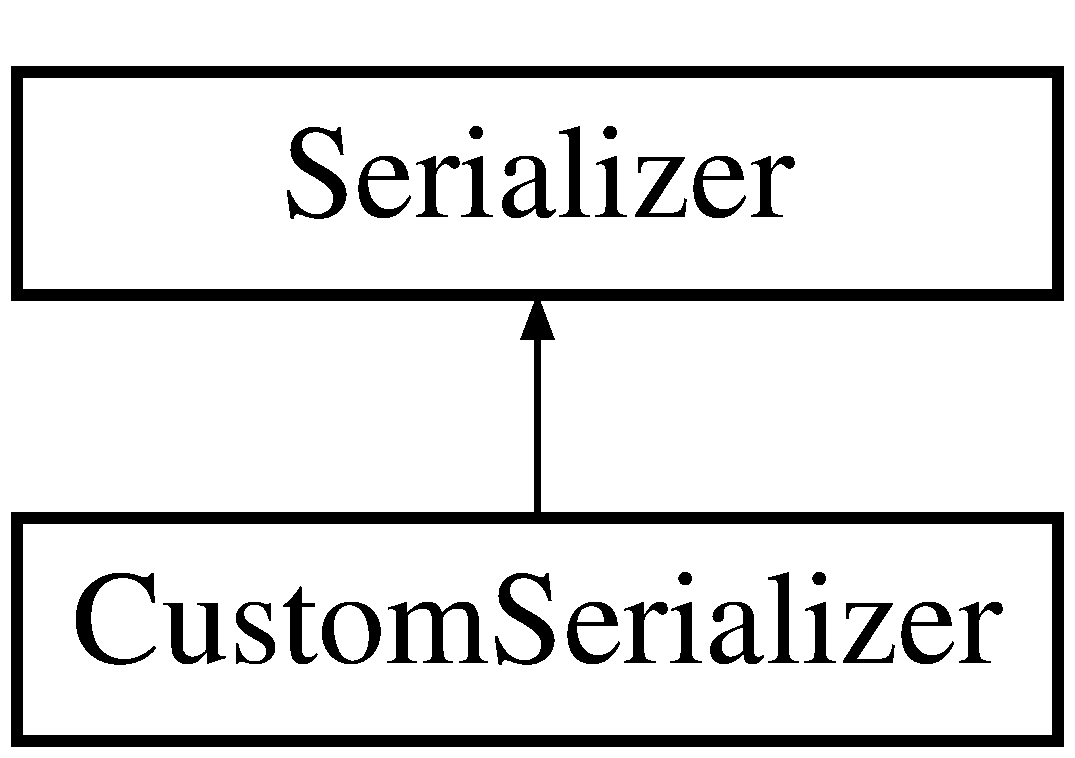
\includegraphics[height=2.000000cm]{classCustomSerializer}
\end{center}
\end{figure}
\subsection*{Public Member Functions}
\begin{DoxyCompactItemize}
\item 
\mbox{\hyperlink{classTransaction}{Transaction}} $\ast$ \mbox{\hyperlink{classCustomSerializer_abff58f1a955c2f399127b7e3cae23223}{unserialize\+Transaction}} (std\+::string transaction, const char $\ast$key) const override
\item 
virtual char $\ast$ \mbox{\hyperlink{classSerializer_a5cfe31eb70f4d0c92f2d68c22f39e885}{serialize}} (const \mbox{\hyperlink{classComponent}{Component}} $\ast$component, const char $\ast$encoding) const
\item 
virtual char $\ast$ \mbox{\hyperlink{classSerializer_a38bec517fb3b3cc0778c75b807cb930c}{serialize}} (\mbox{\hyperlink{classElement}{Element}} $\ast$element, const char $\ast$encoding) const
\item 
virtual \mbox{\hyperlink{classBlock}{Block}} $\ast$ \mbox{\hyperlink{classSerializer_a423fb7c43ca9c23e07000dba0c5a432a}{unserialize\+Block}} (std\+::string block, const char $\ast$encoding) const
\item 
virtual \mbox{\hyperlink{classMessage}{Message}} $\ast$ \mbox{\hyperlink{classSerializer_a1d16df9f35a7580da06a497dfbddffe8}{unserialize\+Message}} (std\+::string message, const char $\ast$encoding) const
\item 
virtual \mbox{\hyperlink{classMetadata}{Metadata}} $\ast$ \mbox{\hyperlink{classSerializer_a64b858f0c2968e888cf796b6f09eed7b}{unserialize\+Metadata}} (std\+::string message, const char $\ast$encoding) const
\item 
\mbox{\hyperlink{classElementObject}{Element\+Object}} $\ast$ \mbox{\hyperlink{classSerializer_ab3bcdbd49167109de13e03878337018a}{get\+Element}} (std\+::string str, const char $\ast$encoding) const
\item 
void \mbox{\hyperlink{classSerializer_aee483f1845ca1b7f7ac4243de9902750}{set\+\_\+serializer}} (\mbox{\hyperlink{classContentCreator}{Content\+Creator}} $\ast$creator)
\item 
void \mbox{\hyperlink{classSerializer_a74ea868b820b4a8472da98c0045418fa}{set\+\_\+unserializer}} (\mbox{\hyperlink{classContentParser}{Content\+Parser}} $\ast$parser)
\end{DoxyCompactItemize}
\subsection*{Protected Attributes}
\begin{DoxyCompactItemize}
\item 
\mbox{\hyperlink{classFactory}{Factory}}$<$ \mbox{\hyperlink{classContentCreator}{Content\+Creator}} $\ast$ $>$ \mbox{\hyperlink{classSerializer_a7d26e865966b304350653b1246ec3340}{creators}}
\item 
\mbox{\hyperlink{classFactory}{Factory}}$<$ \mbox{\hyperlink{classContentParser}{Content\+Parser}} $\ast$ $>$ \mbox{\hyperlink{classSerializer_a96f96c01e6a471513669621751591fd9}{parsers}}
\end{DoxyCompactItemize}


\subsection{Member Function Documentation}
\mbox{\Hypertarget{classSerializer_ab3bcdbd49167109de13e03878337018a}\label{classSerializer_ab3bcdbd49167109de13e03878337018a}} 
\index{Custom\+Serializer@{Custom\+Serializer}!get\+Element@{get\+Element}}
\index{get\+Element@{get\+Element}!Custom\+Serializer@{Custom\+Serializer}}
\subsubsection{\texorpdfstring{get\+Element()}{getElement()}}
{\footnotesize\ttfamily \mbox{\hyperlink{classElementObject}{Element\+Object}} $\ast$ Serializer\+::get\+Element (\begin{DoxyParamCaption}\item[{std\+::string}]{str,  }\item[{const char $\ast$}]{encoding }\end{DoxyParamCaption}) const\hspace{0.3cm}{\ttfamily [inherited]}}

Unserialize a given string to obtain a \mbox{\hyperlink{classMetadata}{Metadata}} \begin{DoxySeeAlso}{See also}
\mbox{\hyperlink{classContentParser}{Content\+Parser}} 

\mbox{\hyperlink{classElementObject}{Element\+Object}}
\end{DoxySeeAlso}

\begin{DoxyParams}{Parameters}
{\em str} & the string to be unserialized \\
\hline
{\em encoding} & the key to choose the parser \\
\hline
\end{DoxyParams}
\begin{DoxyReturn}{Returns}
The \mbox{\hyperlink{classElement}{Element}} representation of the string 
\end{DoxyReturn}
\mbox{\Hypertarget{classSerializer_a5cfe31eb70f4d0c92f2d68c22f39e885}\label{classSerializer_a5cfe31eb70f4d0c92f2d68c22f39e885}} 
\index{Custom\+Serializer@{Custom\+Serializer}!serialize@{serialize}}
\index{serialize@{serialize}!Custom\+Serializer@{Custom\+Serializer}}
\subsubsection{\texorpdfstring{serialize()}{serialize()}\hspace{0.1cm}{\footnotesize\ttfamily [1/2]}}
{\footnotesize\ttfamily char $\ast$ Serializer\+::serialize (\begin{DoxyParamCaption}\item[{const \mbox{\hyperlink{classComponent}{Component}} $\ast$}]{component,  }\item[{const char $\ast$}]{encoding }\end{DoxyParamCaption}) const\hspace{0.3cm}{\ttfamily [virtual]}, {\ttfamily [inherited]}}

Serialize a \mbox{\hyperlink{classComponent}{Component}} object \begin{DoxySeeAlso}{See also}
\mbox{\hyperlink{classComponent}{Component}} 

\mbox{\hyperlink{classContentCreator}{Content\+Creator}}
\end{DoxySeeAlso}

\begin{DoxyParams}{Parameters}
{\em component} & the component to be serialized \\
\hline
{\em encoding} & the key to choose the creator \\
\hline
\end{DoxyParams}
\begin{DoxyReturn}{Returns}
the serialized string 
\end{DoxyReturn}
\mbox{\Hypertarget{classSerializer_a38bec517fb3b3cc0778c75b807cb930c}\label{classSerializer_a38bec517fb3b3cc0778c75b807cb930c}} 
\index{Custom\+Serializer@{Custom\+Serializer}!serialize@{serialize}}
\index{serialize@{serialize}!Custom\+Serializer@{Custom\+Serializer}}
\subsubsection{\texorpdfstring{serialize()}{serialize()}\hspace{0.1cm}{\footnotesize\ttfamily [2/2]}}
{\footnotesize\ttfamily char $\ast$ Serializer\+::serialize (\begin{DoxyParamCaption}\item[{\mbox{\hyperlink{classElement}{Element}} $\ast$}]{element,  }\item[{const char $\ast$}]{encoding }\end{DoxyParamCaption}) const\hspace{0.3cm}{\ttfamily [virtual]}, {\ttfamily [inherited]}}

Serialize an \mbox{\hyperlink{classElement}{Element}} object \begin{DoxySeeAlso}{See also}
\mbox{\hyperlink{classElement}{Element}} 

\mbox{\hyperlink{classContentCreator}{Content\+Creator}}
\end{DoxySeeAlso}

\begin{DoxyParams}{Parameters}
{\em element} & the element to be serialized \\
\hline
{\em encoding} & the key to choose the creator \\
\hline
\end{DoxyParams}
\begin{DoxyReturn}{Returns}
the serialized string 
\end{DoxyReturn}
\mbox{\Hypertarget{classSerializer_aee483f1845ca1b7f7ac4243de9902750}\label{classSerializer_aee483f1845ca1b7f7ac4243de9902750}} 
\index{Custom\+Serializer@{Custom\+Serializer}!set\+\_\+serializer@{set\+\_\+serializer}}
\index{set\+\_\+serializer@{set\+\_\+serializer}!Custom\+Serializer@{Custom\+Serializer}}
\subsubsection{\texorpdfstring{set\+\_\+serializer()}{set\_serializer()}}
{\footnotesize\ttfamily void Serializer\+::set\+\_\+serializer (\begin{DoxyParamCaption}\item[{\mbox{\hyperlink{classContentCreator}{Content\+Creator}} $\ast$}]{creator }\end{DoxyParamCaption})\hspace{0.3cm}{\ttfamily [inherited]}}

Add a custom creator to the list \begin{DoxySeeAlso}{See also}
\mbox{\hyperlink{classContentCreator}{Content\+Creator}}
\end{DoxySeeAlso}

\begin{DoxyParams}{Parameters}
{\em creator} & the creator object to use \\
\hline
\end{DoxyParams}
\mbox{\Hypertarget{classSerializer_a74ea868b820b4a8472da98c0045418fa}\label{classSerializer_a74ea868b820b4a8472da98c0045418fa}} 
\index{Custom\+Serializer@{Custom\+Serializer}!set\+\_\+unserializer@{set\+\_\+unserializer}}
\index{set\+\_\+unserializer@{set\+\_\+unserializer}!Custom\+Serializer@{Custom\+Serializer}}
\subsubsection{\texorpdfstring{set\+\_\+unserializer()}{set\_unserializer()}}
{\footnotesize\ttfamily void Serializer\+::set\+\_\+unserializer (\begin{DoxyParamCaption}\item[{\mbox{\hyperlink{classContentParser}{Content\+Parser}} $\ast$}]{parser }\end{DoxyParamCaption})\hspace{0.3cm}{\ttfamily [inherited]}}

Add a custom parser to the list \begin{DoxySeeAlso}{See also}
\mbox{\hyperlink{classContentParser}{Content\+Parser}}
\end{DoxySeeAlso}

\begin{DoxyParams}{Parameters}
{\em creator} & the parser object \\
\hline
\end{DoxyParams}
\mbox{\Hypertarget{classSerializer_a423fb7c43ca9c23e07000dba0c5a432a}\label{classSerializer_a423fb7c43ca9c23e07000dba0c5a432a}} 
\index{Custom\+Serializer@{Custom\+Serializer}!unserialize\+Block@{unserialize\+Block}}
\index{unserialize\+Block@{unserialize\+Block}!Custom\+Serializer@{Custom\+Serializer}}
\subsubsection{\texorpdfstring{unserialize\+Block()}{unserializeBlock()}}
{\footnotesize\ttfamily \mbox{\hyperlink{classBlock}{Block}} $\ast$ Serializer\+::unserialize\+Block (\begin{DoxyParamCaption}\item[{std\+::string}]{block,  }\item[{const char $\ast$}]{encoding }\end{DoxyParamCaption}) const\hspace{0.3cm}{\ttfamily [virtual]}, {\ttfamily [inherited]}}

Unserialize an given string to obtain a \mbox{\hyperlink{classBlock}{Block}} \begin{DoxySeeAlso}{See also}
\mbox{\hyperlink{classContentParser}{Content\+Parser}} 

\mbox{\hyperlink{classBlock}{Block}}
\end{DoxySeeAlso}

\begin{DoxyParams}{Parameters}
{\em block} & the string to be unserialized \\
\hline
{\em encoding} & the key to choose the parser \\
\hline
\end{DoxyParams}
\begin{DoxyReturn}{Returns}
The \mbox{\hyperlink{classBlock}{Block}} object 
\end{DoxyReturn}
\mbox{\Hypertarget{classSerializer_a1d16df9f35a7580da06a497dfbddffe8}\label{classSerializer_a1d16df9f35a7580da06a497dfbddffe8}} 
\index{Custom\+Serializer@{Custom\+Serializer}!unserialize\+Message@{unserialize\+Message}}
\index{unserialize\+Message@{unserialize\+Message}!Custom\+Serializer@{Custom\+Serializer}}
\subsubsection{\texorpdfstring{unserialize\+Message()}{unserializeMessage()}}
{\footnotesize\ttfamily \mbox{\hyperlink{classMessage}{Message}} $\ast$ Serializer\+::unserialize\+Message (\begin{DoxyParamCaption}\item[{std\+::string}]{message,  }\item[{const char $\ast$}]{encoding }\end{DoxyParamCaption}) const\hspace{0.3cm}{\ttfamily [virtual]}, {\ttfamily [inherited]}}

Unserialize an given string to obtain a \mbox{\hyperlink{classMessage}{Message}} \begin{DoxySeeAlso}{See also}
\mbox{\hyperlink{classContentParser}{Content\+Parser}} 

\mbox{\hyperlink{classMessage}{Message}}
\end{DoxySeeAlso}

\begin{DoxyParams}{Parameters}
{\em message} & the string to be unserialized \\
\hline
{\em encoding} & the key to choose the parser \\
\hline
\end{DoxyParams}
\begin{DoxyReturn}{Returns}
The \mbox{\hyperlink{classMessage}{Message}} object 
\end{DoxyReturn}
\mbox{\Hypertarget{classSerializer_a64b858f0c2968e888cf796b6f09eed7b}\label{classSerializer_a64b858f0c2968e888cf796b6f09eed7b}} 
\index{Custom\+Serializer@{Custom\+Serializer}!unserialize\+Metadata@{unserialize\+Metadata}}
\index{unserialize\+Metadata@{unserialize\+Metadata}!Custom\+Serializer@{Custom\+Serializer}}
\subsubsection{\texorpdfstring{unserialize\+Metadata()}{unserializeMetadata()}}
{\footnotesize\ttfamily \mbox{\hyperlink{classMetadata}{Metadata}} $\ast$ Serializer\+::unserialize\+Metadata (\begin{DoxyParamCaption}\item[{std\+::string}]{message,  }\item[{const char $\ast$}]{encoding }\end{DoxyParamCaption}) const\hspace{0.3cm}{\ttfamily [virtual]}, {\ttfamily [inherited]}}

Unserialize an given string to obtain a \mbox{\hyperlink{classMetadata}{Metadata}} \begin{DoxySeeAlso}{See also}
\mbox{\hyperlink{classContentParser}{Content\+Parser}} 

\mbox{\hyperlink{classMetadata}{Metadata}}
\end{DoxySeeAlso}

\begin{DoxyParams}{Parameters}
{\em message} & the string to be unserialized \\
\hline
{\em encoding} & the key to choose the parser \\
\hline
\end{DoxyParams}
\begin{DoxyReturn}{Returns}
The \mbox{\hyperlink{classMetadata}{Metadata}} object 
\end{DoxyReturn}
\mbox{\Hypertarget{classCustomSerializer_abff58f1a955c2f399127b7e3cae23223}\label{classCustomSerializer_abff58f1a955c2f399127b7e3cae23223}} 
\index{Custom\+Serializer@{Custom\+Serializer}!unserialize\+Transaction@{unserialize\+Transaction}}
\index{unserialize\+Transaction@{unserialize\+Transaction}!Custom\+Serializer@{Custom\+Serializer}}
\subsubsection{\texorpdfstring{unserialize\+Transaction()}{unserializeTransaction()}}
{\footnotesize\ttfamily \mbox{\hyperlink{classTransaction}{Transaction}} $\ast$ Custom\+Serializer\+::unserialize\+Transaction (\begin{DoxyParamCaption}\item[{std\+::string}]{transaction,  }\item[{const char $\ast$}]{encoding }\end{DoxyParamCaption}) const\hspace{0.3cm}{\ttfamily [override]}, {\ttfamily [virtual]}}

Unserialize an given string to obtain a \mbox{\hyperlink{classTransaction}{Transaction}} (needs override) \begin{DoxySeeAlso}{See also}
\mbox{\hyperlink{classContentParser}{Content\+Parser}} 

\mbox{\hyperlink{classTransaction}{Transaction}}
\end{DoxySeeAlso}

\begin{DoxyParams}{Parameters}
{\em transaction} & the string to be unserialized \\
\hline
{\em encoding} & the key to choose the parser \\
\hline
\end{DoxyParams}
\begin{DoxyReturn}{Returns}
The \mbox{\hyperlink{classTransaction}{Transaction}} object 
\end{DoxyReturn}


Reimplemented from \mbox{\hyperlink{classSerializer_ab5fa979a8486be6f49ad10f4810509d7}{Serializer}}.



\subsection{Member Data Documentation}
\mbox{\Hypertarget{classSerializer_a7d26e865966b304350653b1246ec3340}\label{classSerializer_a7d26e865966b304350653b1246ec3340}} 
\index{Custom\+Serializer@{Custom\+Serializer}!creators@{creators}}
\index{creators@{creators}!Custom\+Serializer@{Custom\+Serializer}}
\subsubsection{\texorpdfstring{creators}{creators}}
{\footnotesize\ttfamily \mbox{\hyperlink{classFactory}{Factory}}$<$\mbox{\hyperlink{classContentCreator}{Content\+Creator}}$\ast$$>$ Serializer\+::creators\hspace{0.3cm}{\ttfamily [protected]}, {\ttfamily [inherited]}}

The factory of different creators \begin{DoxySeeAlso}{See also}
\mbox{\hyperlink{classFactory}{Factory}} 

\mbox{\hyperlink{classContentCreator}{Content\+Creator}} 
\end{DoxySeeAlso}
\mbox{\Hypertarget{classSerializer_a96f96c01e6a471513669621751591fd9}\label{classSerializer_a96f96c01e6a471513669621751591fd9}} 
\index{Custom\+Serializer@{Custom\+Serializer}!parsers@{parsers}}
\index{parsers@{parsers}!Custom\+Serializer@{Custom\+Serializer}}
\subsubsection{\texorpdfstring{parsers}{parsers}}
{\footnotesize\ttfamily \mbox{\hyperlink{classFactory}{Factory}}$<$\mbox{\hyperlink{classContentParser}{Content\+Parser}}$\ast$$>$ Serializer\+::parsers\hspace{0.3cm}{\ttfamily [protected]}, {\ttfamily [inherited]}}

The factory of different parsers \begin{DoxySeeAlso}{See also}
\mbox{\hyperlink{classFactory}{Factory}} 

\mbox{\hyperlink{classContentParser}{Content\+Parser}} 
\end{DoxySeeAlso}


The documentation for this class was generated from the following files\+:\begin{DoxyCompactItemize}
\item 
serializer/Custom\+Serializer.\+h\item 
serializer/Custom\+Serializer.\+cpp\end{DoxyCompactItemize}

\hypertarget{classDatabase}{}\section{Database Class Reference}
\label{classDatabase}\index{Database@{Database}}
\subsection*{Public Member Functions}
\begin{DoxyCompactItemize}
\item 
\mbox{\Hypertarget{classDatabase_ab00a6ec54927a6a80f5c09a926ee4611}\label{classDatabase_ab00a6ec54927a6a80f5c09a926ee4611}} 
{\bfseries Database} (\mbox{\hyperlink{classReward}{Reward}} $\ast$r)
\item 
\mbox{\Hypertarget{classDatabase_a53798837997415704f1ce331aa93eda9}\label{classDatabase_a53798837997415704f1ce331aa93eda9}} 
\mbox{\hyperlink{classDatabase}{Database}} \& {\bfseries operator=} (\mbox{\hyperlink{classDatabase}{Database}} const \&d)
\item 
\mbox{\Hypertarget{classDatabase_a194c4d15c58a98ce7156afd33e64ae16}\label{classDatabase_a194c4d15c58a98ce7156afd33e64ae16}} 
\mbox{\hyperlink{classRow}{Row}} $\ast$ {\bfseries get} (std\+::string key)
\item 
\mbox{\Hypertarget{classDatabase_a3e8f5125a0db0c76d35bd4a36894e203}\label{classDatabase_a3e8f5125a0db0c76d35bd4a36894e203}} 
\mbox{\hyperlink{classRow}{Row}} $\ast$ {\bfseries reward} (std\+::string winner)
\end{DoxyCompactItemize}
\subsection*{Friends}
\begin{DoxyCompactItemize}
\item 
\mbox{\Hypertarget{classDatabase_a65813570c30a3e0656fa523793ff1b86}\label{classDatabase_a65813570c30a3e0656fa523793ff1b86}} 
class {\bfseries Chain}
\end{DoxyCompactItemize}


The documentation for this class was generated from the following file\+:\begin{DoxyCompactItemize}
\item 
block\+\_\+chain/chain/state/Database.\+h\end{DoxyCompactItemize}

\hypertarget{classElement}{}\section{Element Class Reference}
\label{classElement}\index{Element@{Element}}


{\ttfamily \#include $<$Element.\+h$>$}

Inheritance diagram for Element\+:\begin{figure}[H]
\begin{center}
\leavevmode
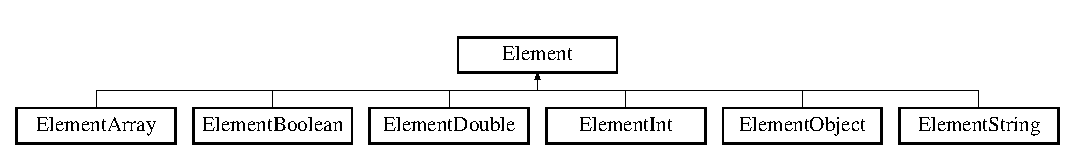
\includegraphics[height=1.696970cm]{classElement}
\end{center}
\end{figure}
\subsection*{Public Member Functions}
\begin{DoxyCompactItemize}
\item 
virtual void \mbox{\hyperlink{classElement_ab468bd37a9558f5227837a9236bc9e4b}{read}} (std\+::string \&text, const \mbox{\hyperlink{classContentReader}{Content\+Reader}} $\ast$reader)
\item 
virtual \mbox{\hyperlink{classElement_aa153979c5d46fff8e2b9ee8b48dd863f}{$\sim$\+Element}} ()=default
\end{DoxyCompactItemize}


\subsection{Detailed Description}
The \mbox{\hyperlink{classElement}{Element}} base class for serialization

\begin{DoxyAuthor}{Author}
Mathieu Lochet 
\end{DoxyAuthor}
\begin{DoxyVersion}{Version}
1 
\end{DoxyVersion}


\subsection{Constructor \& Destructor Documentation}
\mbox{\Hypertarget{classElement_aa153979c5d46fff8e2b9ee8b48dd863f}\label{classElement_aa153979c5d46fff8e2b9ee8b48dd863f}} 
\index{Element@{Element}!````~Element@{$\sim$\+Element}}
\index{````~Element@{$\sim$\+Element}!Element@{Element}}
\subsubsection{\texorpdfstring{$\sim$\+Element()}{~Element()}}
{\footnotesize\ttfamily virtual Element\+::$\sim$\+Element (\begin{DoxyParamCaption}{ }\end{DoxyParamCaption})\hspace{0.3cm}{\ttfamily [virtual]}, {\ttfamily [default]}}

Default destructor 

\subsection{Member Function Documentation}
\mbox{\Hypertarget{classElement_ab468bd37a9558f5227837a9236bc9e4b}\label{classElement_ab468bd37a9558f5227837a9236bc9e4b}} 
\index{Element@{Element}!read@{read}}
\index{read@{read}!Element@{Element}}
\subsubsection{\texorpdfstring{read()}{read()}}
{\footnotesize\ttfamily virtual void Element\+::read (\begin{DoxyParamCaption}\item[{std\+::string \&}]{text,  }\item[{const \mbox{\hyperlink{classContentReader}{Content\+Reader}} $\ast$}]{reader }\end{DoxyParamCaption})\hspace{0.3cm}{\ttfamily [inline]}, {\ttfamily [virtual]}}

Used with polymorphism, lead the readers in the right direction for both text and \mbox{\hyperlink{classElement}{Element}} creation. \begin{DoxySeeAlso}{See also}
\mbox{\hyperlink{classContentReader}{Content\+Reader}}
\end{DoxySeeAlso}

\begin{DoxyParams}{Parameters}
{\em text} & the current used text by the reader \\
\hline
{\em reader} & the current reader used \\
\hline
\end{DoxyParams}


Reimplemented in \mbox{\hyperlink{classElementObject_a2217d9754771964af5e590a5fabe2c4e}{Element\+Object}}, \mbox{\hyperlink{classElementArray_a5353c82d5c132acdad69858884e3e334}{Element\+Array}}, \mbox{\hyperlink{classElementBoolean_afca7544719a8e13fb38f62d57df343b7}{Element\+Boolean}}, \mbox{\hyperlink{classElementString_a781fe545117610d945772b240f24ac44}{Element\+String}}, \mbox{\hyperlink{classElementDouble_a11bf3651edd2cbcdf04610b113accf90}{Element\+Double}}, and \mbox{\hyperlink{classElementInt_ab5a7d87743dbdc52910c59bc4b93e6da}{Element\+Int}}.



The documentation for this class was generated from the following file\+:\begin{DoxyCompactItemize}
\item 
block\+\_\+chain/utils/serialization/Element.\+h\end{DoxyCompactItemize}

\hypertarget{classElementArray}{}\section{Element\+Array Class Reference}
\label{classElementArray}\index{Element\+Array@{Element\+Array}}


{\ttfamily \#include $<$Element.\+h$>$}

Inheritance diagram for Element\+Array\+:\begin{figure}[H]
\begin{center}
\leavevmode
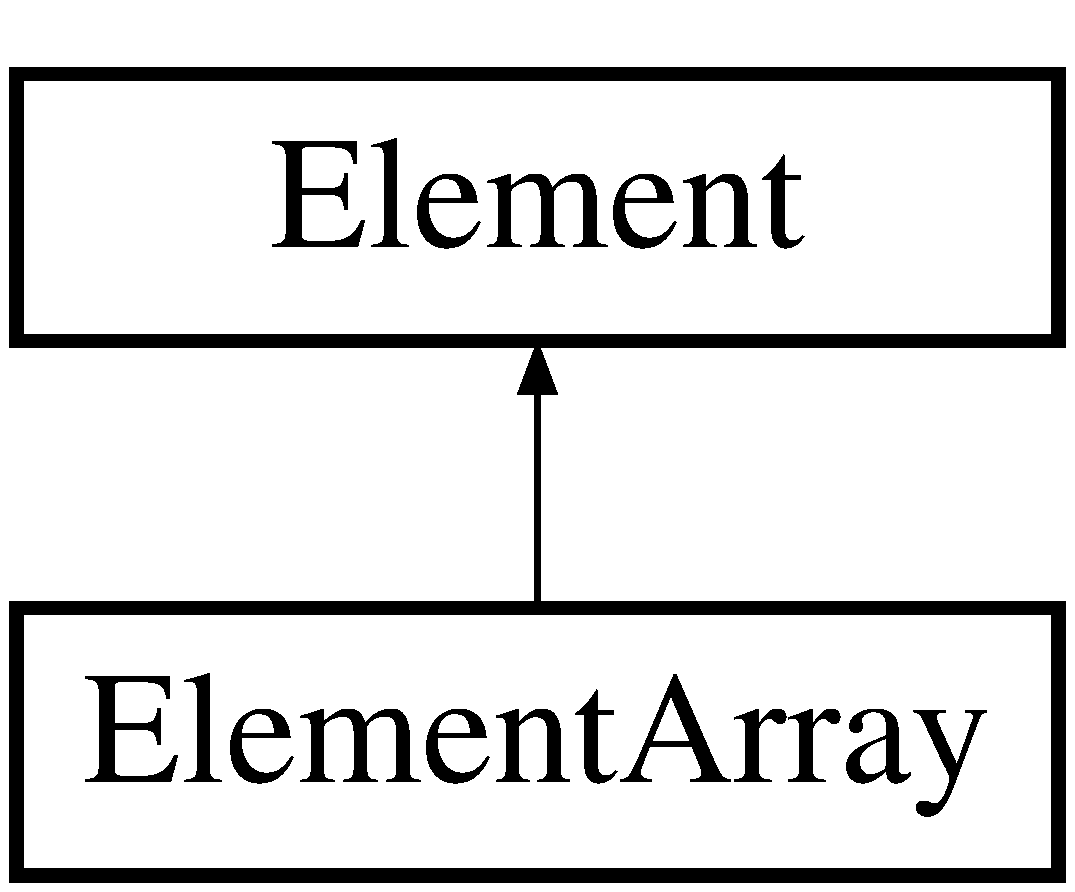
\includegraphics[height=2.000000cm]{classElementArray}
\end{center}
\end{figure}
\subsection*{Public Member Functions}
\begin{DoxyCompactItemize}
\item 
void \mbox{\hyperlink{classElementArray_a5353c82d5c132acdad69858884e3e334}{read}} (std\+::string \&text, const \mbox{\hyperlink{classContentReader}{Content\+Reader}} $\ast$parser) override
\item 
\mbox{\hyperlink{classElementArray}{Element\+Array}} $\ast$ \mbox{\hyperlink{classElementArray_aff62f7af32e8440015b8dd297749b6c6}{add}} (\mbox{\hyperlink{classElement}{Element}} $\ast$value)
\item 
\mbox{\hyperlink{classElementArray_a30d544b599922612d29e48a0cc0e3305}{$\sim$\+Element\+Array}} () override
\end{DoxyCompactItemize}
\subsection*{Public Attributes}
\begin{DoxyCompactItemize}
\item 
std\+::vector$<$ \mbox{\hyperlink{classElement}{Element}} $\ast$ $>$ \mbox{\hyperlink{classElementArray_a3d0a8546daca882d59f55413a338be87}{values}}
\end{DoxyCompactItemize}


\subsection{Detailed Description}
The array \mbox{\hyperlink{classElement}{Element}} for serialization

\begin{DoxyAuthor}{Author}
Mathieu Lochet 
\end{DoxyAuthor}
\begin{DoxyVersion}{Version}
1 
\end{DoxyVersion}


\subsection{Constructor \& Destructor Documentation}
\mbox{\Hypertarget{classElementArray_a30d544b599922612d29e48a0cc0e3305}\label{classElementArray_a30d544b599922612d29e48a0cc0e3305}} 
\index{Element\+Array@{Element\+Array}!````~Element\+Array@{$\sim$\+Element\+Array}}
\index{````~Element\+Array@{$\sim$\+Element\+Array}!Element\+Array@{Element\+Array}}
\subsubsection{\texorpdfstring{$\sim$\+Element\+Array()}{~ElementArray()}}
{\footnotesize\ttfamily Element\+Array\+::$\sim$\+Element\+Array (\begin{DoxyParamCaption}{ }\end{DoxyParamCaption})\hspace{0.3cm}{\ttfamily [override]}}

Destructor that free all of the values in the array 

\subsection{Member Function Documentation}
\mbox{\Hypertarget{classElementArray_aff62f7af32e8440015b8dd297749b6c6}\label{classElementArray_aff62f7af32e8440015b8dd297749b6c6}} 
\index{Element\+Array@{Element\+Array}!add@{add}}
\index{add@{add}!Element\+Array@{Element\+Array}}
\subsubsection{\texorpdfstring{add()}{add()}}
{\footnotesize\ttfamily \mbox{\hyperlink{classElementArray}{Element\+Array}} $\ast$ Element\+Array\+::add (\begin{DoxyParamCaption}\item[{\mbox{\hyperlink{classElement}{Element}} $\ast$}]{value }\end{DoxyParamCaption})}

Add an \mbox{\hyperlink{classElement}{Element}} to the array. Works as a builder \begin{DoxySeeAlso}{See also}
\mbox{\hyperlink{classElement}{Element}}
\end{DoxySeeAlso}

\begin{DoxyParams}{Parameters}
{\em value} & the new value to append to the array \\
\hline
\end{DoxyParams}
\begin{DoxyReturn}{Returns}
the \mbox{\hyperlink{classElementArray}{Element\+Array}} to be used as a builder 
\end{DoxyReturn}
\mbox{\Hypertarget{classElementArray_a5353c82d5c132acdad69858884e3e334}\label{classElementArray_a5353c82d5c132acdad69858884e3e334}} 
\index{Element\+Array@{Element\+Array}!read@{read}}
\index{read@{read}!Element\+Array@{Element\+Array}}
\subsubsection{\texorpdfstring{read()}{read()}}
{\footnotesize\ttfamily void Element\+Array\+::read (\begin{DoxyParamCaption}\item[{std\+::string \&}]{text,  }\item[{const \mbox{\hyperlink{classContentReader}{Content\+Reader}} $\ast$}]{reader }\end{DoxyParamCaption})\hspace{0.3cm}{\ttfamily [override]}, {\ttfamily [virtual]}}

Used with polymorphism, lead the readers in the right direction for both text and \mbox{\hyperlink{classElement}{Element}} creation. \begin{DoxySeeAlso}{See also}
\mbox{\hyperlink{classContentReader}{Content\+Reader}}
\end{DoxySeeAlso}

\begin{DoxyParams}{Parameters}
{\em text} & the current used text by the reader \\
\hline
{\em reader} & the current reader used \\
\hline
\end{DoxyParams}


Reimplemented from \mbox{\hyperlink{classElement_ab468bd37a9558f5227837a9236bc9e4b}{Element}}.



\subsection{Member Data Documentation}
\mbox{\Hypertarget{classElementArray_a3d0a8546daca882d59f55413a338be87}\label{classElementArray_a3d0a8546daca882d59f55413a338be87}} 
\index{Element\+Array@{Element\+Array}!values@{values}}
\index{values@{values}!Element\+Array@{Element\+Array}}
\subsubsection{\texorpdfstring{values}{values}}
{\footnotesize\ttfamily std\+::vector$<$\mbox{\hyperlink{classElement}{Element}}$\ast$$>$ Element\+Array\+::values}

The list of Elements to be used in serialization \begin{DoxySeeAlso}{See also}
\mbox{\hyperlink{classElement}{Element}} 
\end{DoxySeeAlso}


The documentation for this class was generated from the following files\+:\begin{DoxyCompactItemize}
\item 
block\+\_\+chain/utils/serialization/Element.\+h\item 
block\+\_\+chain/utils/serialization/Element.\+cpp\end{DoxyCompactItemize}

\hypertarget{classElementBoolean}{}\section{Element\+Boolean Class Reference}
\label{classElementBoolean}\index{Element\+Boolean@{Element\+Boolean}}


{\ttfamily \#include $<$Element.\+h$>$}

Inheritance diagram for Element\+Boolean\+:\begin{figure}[H]
\begin{center}
\leavevmode
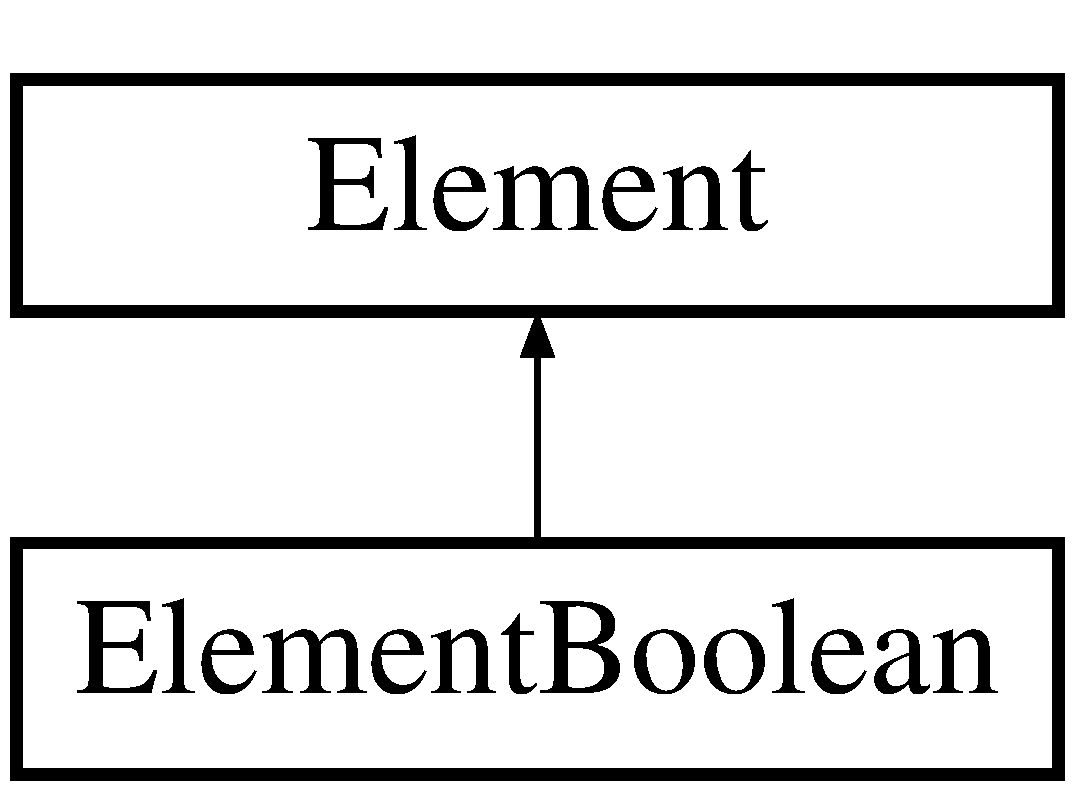
\includegraphics[height=2.000000cm]{classElementBoolean}
\end{center}
\end{figure}
\subsection*{Public Member Functions}
\begin{DoxyCompactItemize}
\item 
void \mbox{\hyperlink{classElementBoolean_afca7544719a8e13fb38f62d57df343b7}{read}} (std\+::string \&text, const \mbox{\hyperlink{classContentReader}{Content\+Reader}} $\ast$parser) override
\end{DoxyCompactItemize}
\subsection*{Public Attributes}
\begin{DoxyCompactItemize}
\item 
bool \mbox{\hyperlink{classElementBoolean_a470b48a447bd7704bbf57fc42d78a4e2}{value}}
\end{DoxyCompactItemize}


\subsection{Detailed Description}
The boolean \mbox{\hyperlink{classElement}{Element}} for serialization

\begin{DoxyAuthor}{Author}
Mathieu Lochet 
\end{DoxyAuthor}
\begin{DoxyVersion}{Version}
1 
\end{DoxyVersion}


\subsection{Member Function Documentation}
\mbox{\Hypertarget{classElementBoolean_afca7544719a8e13fb38f62d57df343b7}\label{classElementBoolean_afca7544719a8e13fb38f62d57df343b7}} 
\index{Element\+Boolean@{Element\+Boolean}!read@{read}}
\index{read@{read}!Element\+Boolean@{Element\+Boolean}}
\subsubsection{\texorpdfstring{read()}{read()}}
{\footnotesize\ttfamily void Element\+Boolean\+::read (\begin{DoxyParamCaption}\item[{std\+::string \&}]{text,  }\item[{const \mbox{\hyperlink{classContentReader}{Content\+Reader}} $\ast$}]{reader }\end{DoxyParamCaption})\hspace{0.3cm}{\ttfamily [override]}, {\ttfamily [virtual]}}

Used with polymorphism, lead the readers in the right direction for both text and \mbox{\hyperlink{classElement}{Element}} creation. \begin{DoxySeeAlso}{See also}
\mbox{\hyperlink{classContentReader}{Content\+Reader}}
\end{DoxySeeAlso}

\begin{DoxyParams}{Parameters}
{\em text} & the current used text by the reader \\
\hline
{\em reader} & the current reader used \\
\hline
\end{DoxyParams}


Reimplemented from \mbox{\hyperlink{classElement_ab468bd37a9558f5227837a9236bc9e4b}{Element}}.



\subsection{Member Data Documentation}
\mbox{\Hypertarget{classElementBoolean_a470b48a447bd7704bbf57fc42d78a4e2}\label{classElementBoolean_a470b48a447bd7704bbf57fc42d78a4e2}} 
\index{Element\+Boolean@{Element\+Boolean}!value@{value}}
\index{value@{value}!Element\+Boolean@{Element\+Boolean}}
\subsubsection{\texorpdfstring{value}{value}}
{\footnotesize\ttfamily bool Element\+Boolean\+::value}

The boolean value to be used in serialization 

The documentation for this class was generated from the following files\+:\begin{DoxyCompactItemize}
\item 
block\+\_\+chain/utils/serialization/Element.\+h\item 
block\+\_\+chain/utils/serialization/Element.\+cpp\end{DoxyCompactItemize}

\hypertarget{classElementCreator}{}\section{Element\+Creator Class Reference}
\label{classElementCreator}\index{Element\+Creator@{Element\+Creator}}


{\ttfamily \#include $<$Parser.\+h$>$}

\subsection*{Static Public Member Functions}
\begin{DoxyCompactItemize}
\item 
static \mbox{\hyperlink{classElementInt}{Element\+Int}} $\ast$ \mbox{\hyperlink{classElementCreator_a4d2ee7d169ec568eb76e41dc0baaf314}{create}} (int value)
\item 
static \mbox{\hyperlink{classElementInt}{Element\+Int}} $\ast$ \mbox{\hyperlink{classElementCreator_ab7938321c7e51a63747c94b283ff2978}{create}} (long long int value)
\item 
static \mbox{\hyperlink{classElementDouble}{Element\+Double}} $\ast$ \mbox{\hyperlink{classElementCreator_a4654c6b5d2431bde10d9652146ad43a1}{create}} (double value)
\item 
static \mbox{\hyperlink{classElementString}{Element\+String}} $\ast$ \mbox{\hyperlink{classElementCreator_a85bfd97a051e5ae5a790b919aa28fee2}{create}} (const char $\ast$value)
\item 
static \mbox{\hyperlink{classElementString}{Element\+String}} $\ast$ \mbox{\hyperlink{classElementCreator_ab1342c3ed8561bf9ad762c7446a3f4e8}{create}} (std\+::string value)
\item 
static \mbox{\hyperlink{classElementBoolean}{Element\+Boolean}} $\ast$ \mbox{\hyperlink{classElementCreator_aca695a65aa4ef18a480ed380d07e7adf}{create}} (bool value)
\item 
static \mbox{\hyperlink{classElementArray}{Element\+Array}} $\ast$ \mbox{\hyperlink{classElementCreator_a997d880e54dc5282f795c741117088c7}{array}} ()
\item 
static \mbox{\hyperlink{classElementObject}{Element\+Object}} $\ast$ \mbox{\hyperlink{classElementCreator_a9ecb3456bf27d6f9b3c9f5f8130cfe63}{object}} ()
\item 
static \mbox{\hyperlink{classElementArray}{Element\+Array}} $\ast$ \mbox{\hyperlink{classElementCreator_a2e31122026b0cbc70196b5c299c33816}{add}} (\mbox{\hyperlink{classElementArray}{Element\+Array}} $\ast$e, \mbox{\hyperlink{classElement}{Element}} $\ast$value)
\item 
static \mbox{\hyperlink{classElementObject}{Element\+Object}} $\ast$ \mbox{\hyperlink{classElementCreator_a741ad4af271f1dcc1a113d2f49189bb4}{put}} (\mbox{\hyperlink{classElementObject}{Element\+Object}} $\ast$e, const char $\ast$key, \mbox{\hyperlink{classElement}{Element}} $\ast$value)
\end{DoxyCompactItemize}


\subsection{Detailed Description}
The \mbox{\hyperlink{classElement}{Element}} creator class is a static factory that can generates Elements for different primitive types. \begin{DoxySeeAlso}{See also}
\mbox{\hyperlink{classElementInt}{Element\+Int}} 

\mbox{\hyperlink{classElementDouble}{Element\+Double}} 

\mbox{\hyperlink{classElementString}{Element\+String}} 

\mbox{\hyperlink{classElementBoolean}{Element\+Boolean}} 

\mbox{\hyperlink{classElementArray}{Element\+Array}} 

\mbox{\hyperlink{classElementObject}{Element\+Object}}
\end{DoxySeeAlso}
\begin{DoxyAuthor}{Author}
Mathieu Lochet 
\end{DoxyAuthor}
\begin{DoxyVersion}{Version}
1 
\end{DoxyVersion}


\subsection{Member Function Documentation}
\mbox{\Hypertarget{classElementCreator_a2e31122026b0cbc70196b5c299c33816}\label{classElementCreator_a2e31122026b0cbc70196b5c299c33816}} 
\index{Element\+Creator@{Element\+Creator}!add@{add}}
\index{add@{add}!Element\+Creator@{Element\+Creator}}
\subsubsection{\texorpdfstring{add()}{add()}}
{\footnotesize\ttfamily \mbox{\hyperlink{classElementArray}{Element\+Array}} $\ast$ Element\+Creator\+::add (\begin{DoxyParamCaption}\item[{\mbox{\hyperlink{classElementArray}{Element\+Array}} $\ast$}]{e,  }\item[{\mbox{\hyperlink{classElement}{Element}} $\ast$}]{value }\end{DoxyParamCaption})\hspace{0.3cm}{\ttfamily [static]}}

Add an \mbox{\hyperlink{classElement}{Element}} to the given \mbox{\hyperlink{classElementArray}{Element\+Array}}. Can be used as a builder. \begin{DoxySeeAlso}{See also}
\mbox{\hyperlink{classElementArray}{Element\+Array}} 

\mbox{\hyperlink{classElement}{Element}}
\end{DoxySeeAlso}

\begin{DoxyParams}{Parameters}
{\em e} & \mbox{\hyperlink{classElementArray}{Element\+Array}} that will be updated \\
\hline
{\em value} & the value that will be appended \\
\hline
\end{DoxyParams}
\begin{DoxyReturn}{Returns}
the given \mbox{\hyperlink{classElementArray}{Element\+Array}} to be used as a builder. 
\end{DoxyReturn}
\mbox{\Hypertarget{classElementCreator_a997d880e54dc5282f795c741117088c7}\label{classElementCreator_a997d880e54dc5282f795c741117088c7}} 
\index{Element\+Creator@{Element\+Creator}!array@{array}}
\index{array@{array}!Element\+Creator@{Element\+Creator}}
\subsubsection{\texorpdfstring{array()}{array()}}
{\footnotesize\ttfamily \mbox{\hyperlink{classElementArray}{Element\+Array}} $\ast$ Element\+Creator\+::array (\begin{DoxyParamCaption}{ }\end{DoxyParamCaption})\hspace{0.3cm}{\ttfamily [static]}}

Generates an \mbox{\hyperlink{classElement}{Element}} representing an array \begin{DoxySeeAlso}{See also}
\mbox{\hyperlink{classElementArray}{Element\+Array}}
\end{DoxySeeAlso}
\begin{DoxyReturn}{Returns}
the generated \mbox{\hyperlink{classElement}{Element}} representation 
\end{DoxyReturn}
\mbox{\Hypertarget{classElementCreator_a4d2ee7d169ec568eb76e41dc0baaf314}\label{classElementCreator_a4d2ee7d169ec568eb76e41dc0baaf314}} 
\index{Element\+Creator@{Element\+Creator}!create@{create}}
\index{create@{create}!Element\+Creator@{Element\+Creator}}
\subsubsection{\texorpdfstring{create()}{create()}\hspace{0.1cm}{\footnotesize\ttfamily [1/6]}}
{\footnotesize\ttfamily \mbox{\hyperlink{classElementInt}{Element\+Int}} $\ast$ Element\+Creator\+::create (\begin{DoxyParamCaption}\item[{int}]{value }\end{DoxyParamCaption})\hspace{0.3cm}{\ttfamily [static]}}

Generates an \mbox{\hyperlink{classElement}{Element}} representing a int \begin{DoxySeeAlso}{See also}
\mbox{\hyperlink{classElementInt}{Element\+Int}}
\end{DoxySeeAlso}

\begin{DoxyParams}{Parameters}
{\em value} & the int value \\
\hline
\end{DoxyParams}
\begin{DoxyReturn}{Returns}
the generated \mbox{\hyperlink{classElement}{Element}} representation 
\end{DoxyReturn}
\mbox{\Hypertarget{classElementCreator_ab7938321c7e51a63747c94b283ff2978}\label{classElementCreator_ab7938321c7e51a63747c94b283ff2978}} 
\index{Element\+Creator@{Element\+Creator}!create@{create}}
\index{create@{create}!Element\+Creator@{Element\+Creator}}
\subsubsection{\texorpdfstring{create()}{create()}\hspace{0.1cm}{\footnotesize\ttfamily [2/6]}}
{\footnotesize\ttfamily \mbox{\hyperlink{classElementInt}{Element\+Int}} $\ast$ Element\+Creator\+::create (\begin{DoxyParamCaption}\item[{long long int}]{value }\end{DoxyParamCaption})\hspace{0.3cm}{\ttfamily [static]}}

Generates an \mbox{\hyperlink{classElement}{Element}} representing a long long int \begin{DoxySeeAlso}{See also}
\mbox{\hyperlink{classElementInt}{Element\+Int}}
\end{DoxySeeAlso}

\begin{DoxyParams}{Parameters}
{\em value} & the int value \\
\hline
\end{DoxyParams}
\begin{DoxyReturn}{Returns}
the generated \mbox{\hyperlink{classElement}{Element}} representation 
\end{DoxyReturn}
\mbox{\Hypertarget{classElementCreator_a4654c6b5d2431bde10d9652146ad43a1}\label{classElementCreator_a4654c6b5d2431bde10d9652146ad43a1}} 
\index{Element\+Creator@{Element\+Creator}!create@{create}}
\index{create@{create}!Element\+Creator@{Element\+Creator}}
\subsubsection{\texorpdfstring{create()}{create()}\hspace{0.1cm}{\footnotesize\ttfamily [3/6]}}
{\footnotesize\ttfamily \mbox{\hyperlink{classElementDouble}{Element\+Double}} $\ast$ Element\+Creator\+::create (\begin{DoxyParamCaption}\item[{double}]{value }\end{DoxyParamCaption})\hspace{0.3cm}{\ttfamily [static]}}

Generates an \mbox{\hyperlink{classElement}{Element}} representing a double \begin{DoxySeeAlso}{See also}
\mbox{\hyperlink{classElementDouble}{Element\+Double}}
\end{DoxySeeAlso}

\begin{DoxyParams}{Parameters}
{\em value} & the double value \\
\hline
\end{DoxyParams}
\begin{DoxyReturn}{Returns}
the generated \mbox{\hyperlink{classElement}{Element}} representation 
\end{DoxyReturn}
\mbox{\Hypertarget{classElementCreator_a85bfd97a051e5ae5a790b919aa28fee2}\label{classElementCreator_a85bfd97a051e5ae5a790b919aa28fee2}} 
\index{Element\+Creator@{Element\+Creator}!create@{create}}
\index{create@{create}!Element\+Creator@{Element\+Creator}}
\subsubsection{\texorpdfstring{create()}{create()}\hspace{0.1cm}{\footnotesize\ttfamily [4/6]}}
{\footnotesize\ttfamily \mbox{\hyperlink{classElementString}{Element\+String}} $\ast$ Element\+Creator\+::create (\begin{DoxyParamCaption}\item[{const char $\ast$}]{value }\end{DoxyParamCaption})\hspace{0.3cm}{\ttfamily [static]}}

Generates an \mbox{\hyperlink{classElement}{Element}} representing a string \begin{DoxySeeAlso}{See also}
\mbox{\hyperlink{classElementString}{Element\+String}}
\end{DoxySeeAlso}

\begin{DoxyParams}{Parameters}
{\em value} & the const char$\ast$ value \\
\hline
\end{DoxyParams}
\begin{DoxyReturn}{Returns}
the generated \mbox{\hyperlink{classElement}{Element}} representation 
\end{DoxyReturn}
\mbox{\Hypertarget{classElementCreator_ab1342c3ed8561bf9ad762c7446a3f4e8}\label{classElementCreator_ab1342c3ed8561bf9ad762c7446a3f4e8}} 
\index{Element\+Creator@{Element\+Creator}!create@{create}}
\index{create@{create}!Element\+Creator@{Element\+Creator}}
\subsubsection{\texorpdfstring{create()}{create()}\hspace{0.1cm}{\footnotesize\ttfamily [5/6]}}
{\footnotesize\ttfamily \mbox{\hyperlink{classElementString}{Element\+String}} $\ast$ Element\+Creator\+::create (\begin{DoxyParamCaption}\item[{std\+::string}]{value }\end{DoxyParamCaption})\hspace{0.3cm}{\ttfamily [static]}}

Generates an \mbox{\hyperlink{classElement}{Element}} representing a string \begin{DoxySeeAlso}{See also}
\mbox{\hyperlink{classElementString}{Element\+String}}
\end{DoxySeeAlso}

\begin{DoxyParams}{Parameters}
{\em value} & the string value \\
\hline
\end{DoxyParams}
\begin{DoxyReturn}{Returns}
the generated \mbox{\hyperlink{classElement}{Element}} representation 
\end{DoxyReturn}
\mbox{\Hypertarget{classElementCreator_aca695a65aa4ef18a480ed380d07e7adf}\label{classElementCreator_aca695a65aa4ef18a480ed380d07e7adf}} 
\index{Element\+Creator@{Element\+Creator}!create@{create}}
\index{create@{create}!Element\+Creator@{Element\+Creator}}
\subsubsection{\texorpdfstring{create()}{create()}\hspace{0.1cm}{\footnotesize\ttfamily [6/6]}}
{\footnotesize\ttfamily \mbox{\hyperlink{classElementBoolean}{Element\+Boolean}} $\ast$ Element\+Creator\+::create (\begin{DoxyParamCaption}\item[{bool}]{value }\end{DoxyParamCaption})\hspace{0.3cm}{\ttfamily [static]}}

Generates an \mbox{\hyperlink{classElement}{Element}} representing a boolean \begin{DoxySeeAlso}{See also}
\mbox{\hyperlink{classElementBoolean}{Element\+Boolean}}
\end{DoxySeeAlso}

\begin{DoxyParams}{Parameters}
{\em value} & the boolean value \\
\hline
\end{DoxyParams}
\begin{DoxyReturn}{Returns}
the generated \mbox{\hyperlink{classElement}{Element}} representation 
\end{DoxyReturn}
\mbox{\Hypertarget{classElementCreator_a9ecb3456bf27d6f9b3c9f5f8130cfe63}\label{classElementCreator_a9ecb3456bf27d6f9b3c9f5f8130cfe63}} 
\index{Element\+Creator@{Element\+Creator}!object@{object}}
\index{object@{object}!Element\+Creator@{Element\+Creator}}
\subsubsection{\texorpdfstring{object()}{object()}}
{\footnotesize\ttfamily \mbox{\hyperlink{classElementObject}{Element\+Object}} $\ast$ Element\+Creator\+::object (\begin{DoxyParamCaption}{ }\end{DoxyParamCaption})\hspace{0.3cm}{\ttfamily [static]}}

Generates an \mbox{\hyperlink{classElement}{Element}} representing an object \begin{DoxySeeAlso}{See also}
\mbox{\hyperlink{classElementObject}{Element\+Object}}
\end{DoxySeeAlso}
\begin{DoxyReturn}{Returns}
the generated \mbox{\hyperlink{classElement}{Element}} representation 
\end{DoxyReturn}
\mbox{\Hypertarget{classElementCreator_a741ad4af271f1dcc1a113d2f49189bb4}\label{classElementCreator_a741ad4af271f1dcc1a113d2f49189bb4}} 
\index{Element\+Creator@{Element\+Creator}!put@{put}}
\index{put@{put}!Element\+Creator@{Element\+Creator}}
\subsubsection{\texorpdfstring{put()}{put()}}
{\footnotesize\ttfamily \mbox{\hyperlink{classElementObject}{Element\+Object}} $\ast$ Element\+Creator\+::put (\begin{DoxyParamCaption}\item[{\mbox{\hyperlink{classElementObject}{Element\+Object}} $\ast$}]{e,  }\item[{const char $\ast$}]{key,  }\item[{\mbox{\hyperlink{classElement}{Element}} $\ast$}]{value }\end{DoxyParamCaption})\hspace{0.3cm}{\ttfamily [static]}}

Add a key and an \mbox{\hyperlink{classElement}{Element}} to the given \mbox{\hyperlink{classElementObject}{Element\+Object}}. Can be used as a builder. \begin{DoxySeeAlso}{See also}
\mbox{\hyperlink{classElementObject}{Element\+Object}} 

\mbox{\hyperlink{classElement}{Element}}
\end{DoxySeeAlso}

\begin{DoxyParams}{Parameters}
{\em e} & \mbox{\hyperlink{classElementObject}{Element\+Object}} that will be updated \\
\hline
{\em key} & the name of the field \\
\hline
{\em value} & the value of the field \\
\hline
\end{DoxyParams}
\begin{DoxyReturn}{Returns}
the given \mbox{\hyperlink{classElementObject}{Element\+Object}} to be used as a builder. 
\end{DoxyReturn}


The documentation for this class was generated from the following files\+:\begin{DoxyCompactItemize}
\item 
block\+\_\+chain/utils/serialization/Parser.\+h\item 
block\+\_\+chain/utils/serialization/Element\+Creator.\+cpp\end{DoxyCompactItemize}

\hypertarget{classElementDouble}{}\section{Element\+Double Class Reference}
\label{classElementDouble}\index{Element\+Double@{Element\+Double}}


{\ttfamily \#include $<$Element.\+h$>$}

Inheritance diagram for Element\+Double\+:\begin{figure}[H]
\begin{center}
\leavevmode
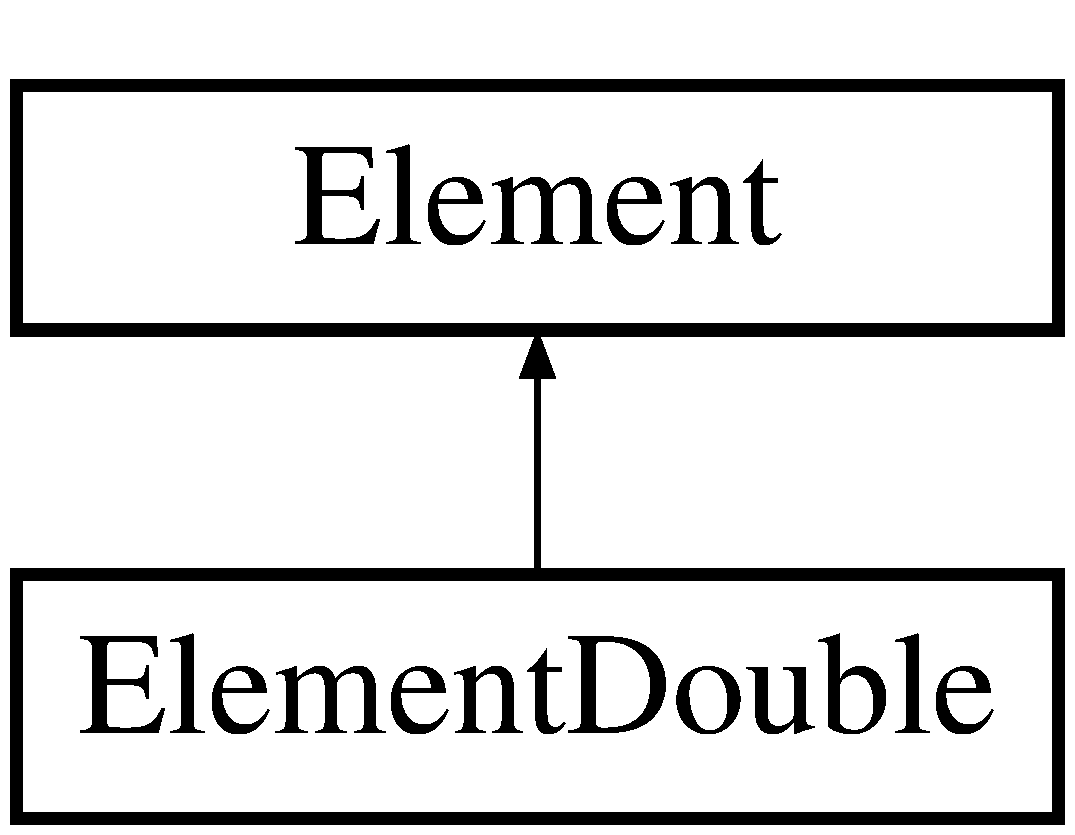
\includegraphics[height=2.000000cm]{classElementDouble}
\end{center}
\end{figure}
\subsection*{Public Member Functions}
\begin{DoxyCompactItemize}
\item 
void \mbox{\hyperlink{classElementDouble_a11bf3651edd2cbcdf04610b113accf90}{read}} (std\+::string \&text, const \mbox{\hyperlink{classContentReader}{Content\+Reader}} $\ast$parser) override
\end{DoxyCompactItemize}
\subsection*{Public Attributes}
\begin{DoxyCompactItemize}
\item 
double \mbox{\hyperlink{classElementDouble_aa04fa64c846076944151db147bcaaa1f}{value}}
\end{DoxyCompactItemize}


\subsection{Detailed Description}
The double \mbox{\hyperlink{classElement}{Element}} for serialization

\begin{DoxyAuthor}{Author}
Mathieu Lochet 
\end{DoxyAuthor}
\begin{DoxyVersion}{Version}
1 
\end{DoxyVersion}


\subsection{Member Function Documentation}
\mbox{\Hypertarget{classElementDouble_a11bf3651edd2cbcdf04610b113accf90}\label{classElementDouble_a11bf3651edd2cbcdf04610b113accf90}} 
\index{Element\+Double@{Element\+Double}!read@{read}}
\index{read@{read}!Element\+Double@{Element\+Double}}
\subsubsection{\texorpdfstring{read()}{read()}}
{\footnotesize\ttfamily void Element\+Double\+::read (\begin{DoxyParamCaption}\item[{std\+::string \&}]{text,  }\item[{const \mbox{\hyperlink{classContentReader}{Content\+Reader}} $\ast$}]{reader }\end{DoxyParamCaption})\hspace{0.3cm}{\ttfamily [override]}, {\ttfamily [virtual]}}

Used with polymorphism, lead the readers in the right direction for both text and \mbox{\hyperlink{classElement}{Element}} creation. \begin{DoxySeeAlso}{See also}
\mbox{\hyperlink{classContentReader}{Content\+Reader}}
\end{DoxySeeAlso}

\begin{DoxyParams}{Parameters}
{\em text} & the current used text by the reader \\
\hline
{\em reader} & the current reader used \\
\hline
\end{DoxyParams}


Reimplemented from \mbox{\hyperlink{classElement_ab468bd37a9558f5227837a9236bc9e4b}{Element}}.



\subsection{Member Data Documentation}
\mbox{\Hypertarget{classElementDouble_aa04fa64c846076944151db147bcaaa1f}\label{classElementDouble_aa04fa64c846076944151db147bcaaa1f}} 
\index{Element\+Double@{Element\+Double}!value@{value}}
\index{value@{value}!Element\+Double@{Element\+Double}}
\subsubsection{\texorpdfstring{value}{value}}
{\footnotesize\ttfamily double Element\+Double\+::value}

The double value to be used in serialization 

The documentation for this class was generated from the following files\+:\begin{DoxyCompactItemize}
\item 
block\+\_\+chain/utils/serialization/Element.\+h\item 
block\+\_\+chain/utils/serialization/Element.\+cpp\end{DoxyCompactItemize}

\hypertarget{classElementInt}{}\section{Element\+Int Class Reference}
\label{classElementInt}\index{Element\+Int@{Element\+Int}}


{\ttfamily \#include $<$Element.\+h$>$}

Inheritance diagram for Element\+Int\+:\begin{figure}[H]
\begin{center}
\leavevmode
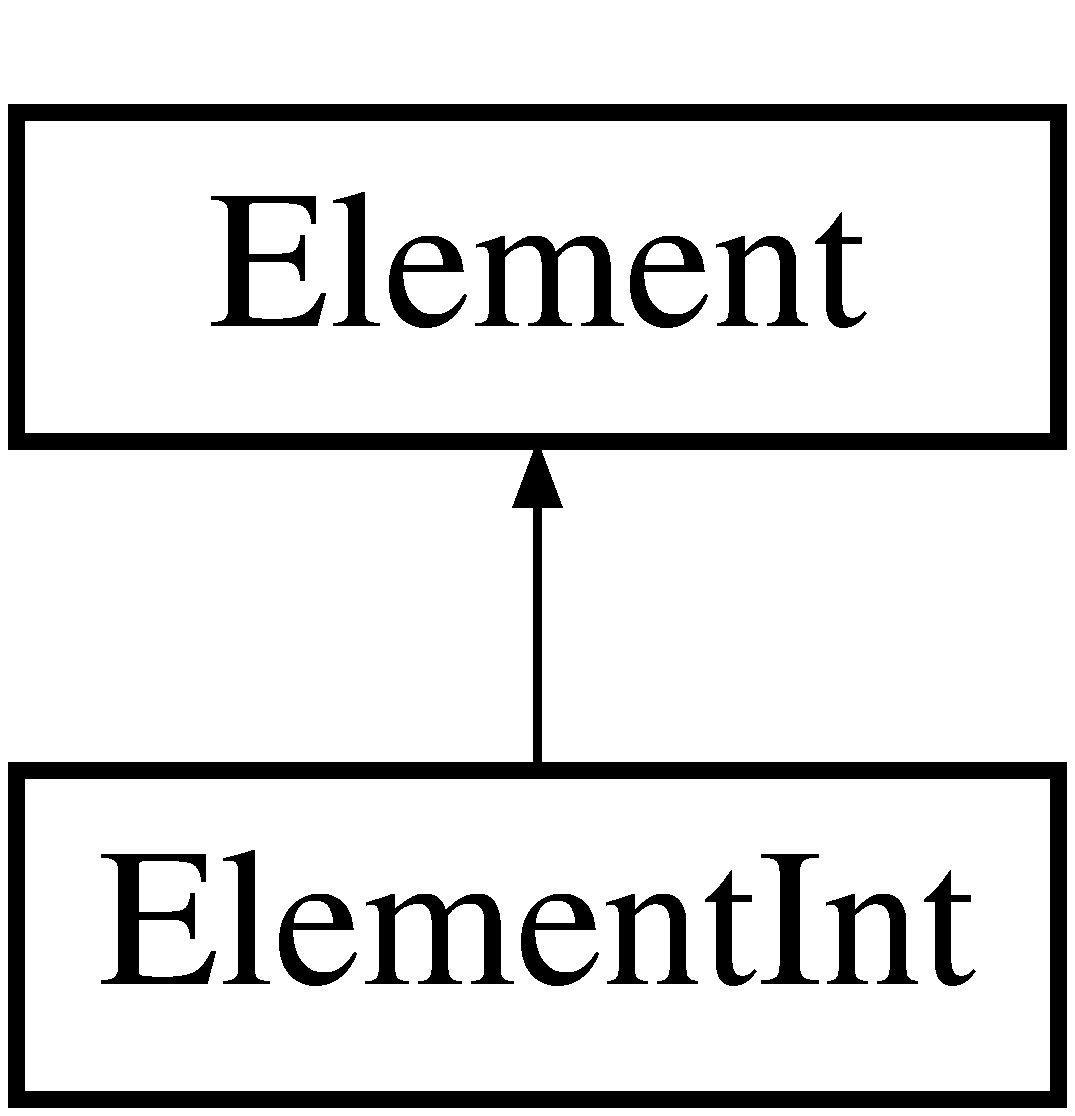
\includegraphics[height=2.000000cm]{classElementInt}
\end{center}
\end{figure}
\subsection*{Public Member Functions}
\begin{DoxyCompactItemize}
\item 
void \mbox{\hyperlink{classElementInt_ab5a7d87743dbdc52910c59bc4b93e6da}{read}} (std\+::string \&text, const \mbox{\hyperlink{classContentReader}{Content\+Reader}} $\ast$parser) override
\end{DoxyCompactItemize}
\subsection*{Public Attributes}
\begin{DoxyCompactItemize}
\item 
long long int \mbox{\hyperlink{classElementInt_ab43f27a056222463dc4bd246337dfa63}{value}}
\end{DoxyCompactItemize}


\subsection{Detailed Description}
The int \mbox{\hyperlink{classElement}{Element}} for serialization

\begin{DoxyAuthor}{Author}
Mathieu Lochet 
\end{DoxyAuthor}
\begin{DoxyVersion}{Version}
1 
\end{DoxyVersion}


\subsection{Member Function Documentation}
\mbox{\Hypertarget{classElementInt_ab5a7d87743dbdc52910c59bc4b93e6da}\label{classElementInt_ab5a7d87743dbdc52910c59bc4b93e6da}} 
\index{Element\+Int@{Element\+Int}!read@{read}}
\index{read@{read}!Element\+Int@{Element\+Int}}
\subsubsection{\texorpdfstring{read()}{read()}}
{\footnotesize\ttfamily void Element\+Int\+::read (\begin{DoxyParamCaption}\item[{std\+::string \&}]{text,  }\item[{const \mbox{\hyperlink{classContentReader}{Content\+Reader}} $\ast$}]{reader }\end{DoxyParamCaption})\hspace{0.3cm}{\ttfamily [override]}, {\ttfamily [virtual]}}

Used with polymorphism, lead the readers in the right direction for both text and \mbox{\hyperlink{classElement}{Element}} creation. \begin{DoxySeeAlso}{See also}
\mbox{\hyperlink{classContentReader}{Content\+Reader}}
\end{DoxySeeAlso}

\begin{DoxyParams}{Parameters}
{\em text} & the current used text by the reader \\
\hline
{\em reader} & the current reader used \\
\hline
\end{DoxyParams}


Reimplemented from \mbox{\hyperlink{classElement_ab468bd37a9558f5227837a9236bc9e4b}{Element}}.



\subsection{Member Data Documentation}
\mbox{\Hypertarget{classElementInt_ab43f27a056222463dc4bd246337dfa63}\label{classElementInt_ab43f27a056222463dc4bd246337dfa63}} 
\index{Element\+Int@{Element\+Int}!value@{value}}
\index{value@{value}!Element\+Int@{Element\+Int}}
\subsubsection{\texorpdfstring{value}{value}}
{\footnotesize\ttfamily long long int Element\+Int\+::value}

The long long int value to be used in serialization 

The documentation for this class was generated from the following files\+:\begin{DoxyCompactItemize}
\item 
block\+\_\+chain/utils/serialization/Element.\+h\item 
block\+\_\+chain/utils/serialization/Element.\+cpp\end{DoxyCompactItemize}

\hypertarget{classElementObject}{}\section{Element\+Object Class Reference}
\label{classElementObject}\index{Element\+Object@{Element\+Object}}


{\ttfamily \#include $<$Element.\+h$>$}

Inheritance diagram for Element\+Object\+:\begin{figure}[H]
\begin{center}
\leavevmode
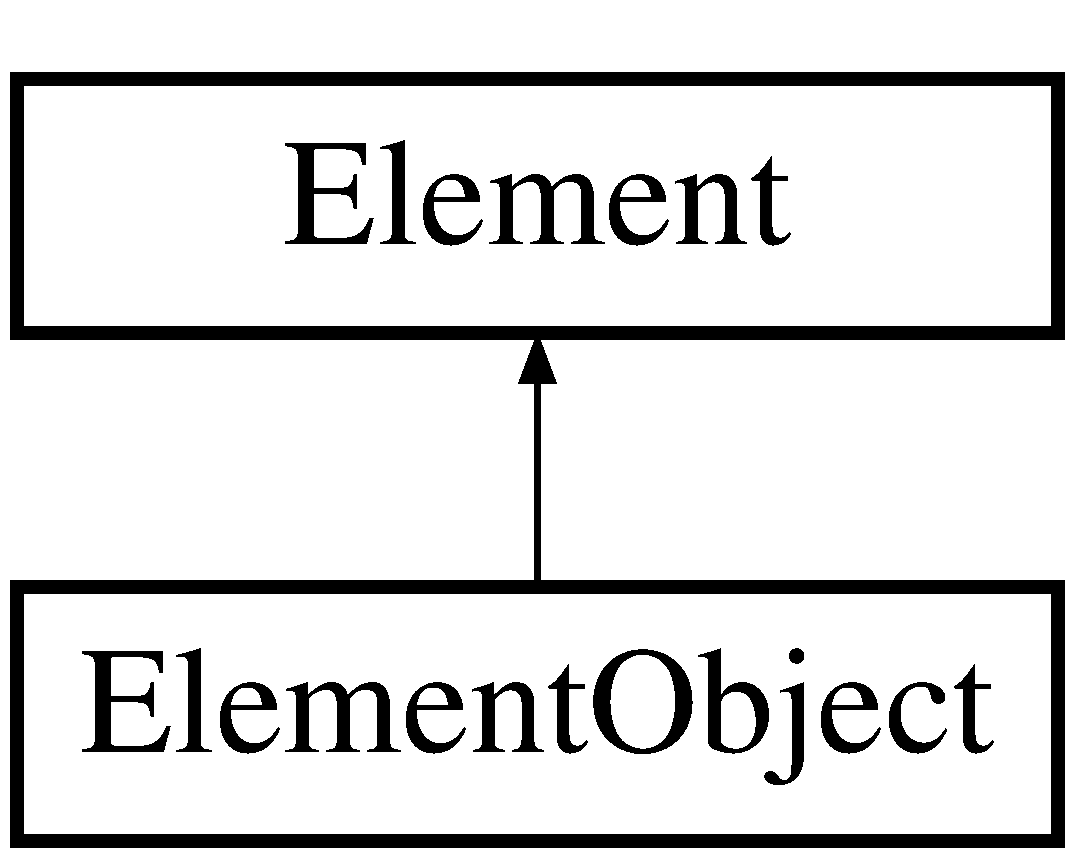
\includegraphics[height=2.000000cm]{classElementObject}
\end{center}
\end{figure}
\subsection*{Public Member Functions}
\begin{DoxyCompactItemize}
\item 
void \mbox{\hyperlink{classElementObject_a7b3a1ef505e63d87ad39309c5ae1b5b3}{get\+Item}} (const char $\ast$key, int $\ast$value)
\item 
void \mbox{\hyperlink{classElementObject_af0ed1f4a16e995e2f66707d3375f7f39}{get\+Item}} (const char $\ast$key, long long int $\ast$value)
\item 
void \mbox{\hyperlink{classElementObject_a78d2c73282624ffed8607d2b8adc3435}{get\+Item}} (const char $\ast$key, bool $\ast$value)
\item 
void \mbox{\hyperlink{classElementObject_a114eb87b32efc8c71c3b14bfc9d121ce}{get\+Item}} (const char $\ast$key, double $\ast$value)
\item 
void \mbox{\hyperlink{classElementObject_a83b8a7f1230171e12f8f3a12326f32a2}{get\+Item}} (const char $\ast$key, \mbox{\hyperlink{classElementObject}{Element\+Object}} $\ast$$\ast$value)
\item 
void \mbox{\hyperlink{classElementObject_adf210b43e30ae63d08c05eb7a46b8c44}{get\+Item}} (const char $\ast$key, \mbox{\hyperlink{classElementArray}{Element\+Array}} $\ast$$\ast$value)
\item 
void \mbox{\hyperlink{classElementObject_a654bd0874175b07f4efa368f97dd82fa}{get\+Item}} (const char $\ast$key, std\+::string $\ast$value)
\item 
void \mbox{\hyperlink{classElementObject_a2217d9754771964af5e590a5fabe2c4e}{read}} (std\+::string \&text, const \mbox{\hyperlink{classContentReader}{Content\+Reader}} $\ast$parser) override
\item 
\mbox{\hyperlink{classElementObject}{Element\+Object}} $\ast$ \mbox{\hyperlink{classElementObject_ab9dd82037b752ab2e6f4e3de53348483}{put}} (const char $\ast$key, \mbox{\hyperlink{classElement}{Element}} $\ast$value)
\item 
\mbox{\hyperlink{classElementObject_a4bec4155f2f99e6ec30e3d44a4d84fa4}{$\sim$\+Element\+Object}} () override
\end{DoxyCompactItemize}
\subsection*{Public Attributes}
\begin{DoxyCompactItemize}
\item 
std\+::map$<$ std\+::string $\ast$, \mbox{\hyperlink{classElement}{Element}} $\ast$, Comparator $>$ \mbox{\hyperlink{classElementObject_afd42a22449d05bcaaf3a194ecb2b4b4c}{values}}
\end{DoxyCompactItemize}


\subsection{Detailed Description}
The object \mbox{\hyperlink{classElement}{Element}} for serialization

\begin{DoxyAuthor}{Author}
Mathieu Lochet 
\end{DoxyAuthor}
\begin{DoxyVersion}{Version}
1 
\end{DoxyVersion}


\subsection{Constructor \& Destructor Documentation}
\mbox{\Hypertarget{classElementObject_a4bec4155f2f99e6ec30e3d44a4d84fa4}\label{classElementObject_a4bec4155f2f99e6ec30e3d44a4d84fa4}} 
\index{Element\+Object@{Element\+Object}!````~Element\+Object@{$\sim$\+Element\+Object}}
\index{````~Element\+Object@{$\sim$\+Element\+Object}!Element\+Object@{Element\+Object}}
\subsubsection{\texorpdfstring{$\sim$\+Element\+Object()}{~ElementObject()}}
{\footnotesize\ttfamily Element\+Object\+::$\sim$\+Element\+Object (\begin{DoxyParamCaption}{ }\end{DoxyParamCaption})\hspace{0.3cm}{\ttfamily [override]}}

Destructor that free all of the values in the map 

\subsection{Member Function Documentation}
\mbox{\Hypertarget{classElementObject_a7b3a1ef505e63d87ad39309c5ae1b5b3}\label{classElementObject_a7b3a1ef505e63d87ad39309c5ae1b5b3}} 
\index{Element\+Object@{Element\+Object}!get\+Item@{get\+Item}}
\index{get\+Item@{get\+Item}!Element\+Object@{Element\+Object}}
\subsubsection{\texorpdfstring{get\+Item()}{getItem()}\hspace{0.1cm}{\footnotesize\ttfamily [1/7]}}
{\footnotesize\ttfamily void Element\+Object\+::get\+Item (\begin{DoxyParamCaption}\item[{const char $\ast$}]{key,  }\item[{int $\ast$}]{value }\end{DoxyParamCaption})}

get an int value from the map


\begin{DoxyParams}{Parameters}
{\em key} & the name of the field \\
\hline
{\em value} & a pointer of int to be updated \\
\hline
\end{DoxyParams}
\mbox{\Hypertarget{classElementObject_af0ed1f4a16e995e2f66707d3375f7f39}\label{classElementObject_af0ed1f4a16e995e2f66707d3375f7f39}} 
\index{Element\+Object@{Element\+Object}!get\+Item@{get\+Item}}
\index{get\+Item@{get\+Item}!Element\+Object@{Element\+Object}}
\subsubsection{\texorpdfstring{get\+Item()}{getItem()}\hspace{0.1cm}{\footnotesize\ttfamily [2/7]}}
{\footnotesize\ttfamily void Element\+Object\+::get\+Item (\begin{DoxyParamCaption}\item[{const char $\ast$}]{key,  }\item[{long long int $\ast$}]{value }\end{DoxyParamCaption})}

get a long long int value from the map


\begin{DoxyParams}{Parameters}
{\em key} & the name of the field \\
\hline
{\em value} & a pointer of long long int to be updated \\
\hline
\end{DoxyParams}
\mbox{\Hypertarget{classElementObject_a78d2c73282624ffed8607d2b8adc3435}\label{classElementObject_a78d2c73282624ffed8607d2b8adc3435}} 
\index{Element\+Object@{Element\+Object}!get\+Item@{get\+Item}}
\index{get\+Item@{get\+Item}!Element\+Object@{Element\+Object}}
\subsubsection{\texorpdfstring{get\+Item()}{getItem()}\hspace{0.1cm}{\footnotesize\ttfamily [3/7]}}
{\footnotesize\ttfamily void Element\+Object\+::get\+Item (\begin{DoxyParamCaption}\item[{const char $\ast$}]{key,  }\item[{bool $\ast$}]{value }\end{DoxyParamCaption})}

get a bool value from the map


\begin{DoxyParams}{Parameters}
{\em key} & the name of the field \\
\hline
{\em value} & a pointer of bool to be updated \\
\hline
\end{DoxyParams}
\mbox{\Hypertarget{classElementObject_a114eb87b32efc8c71c3b14bfc9d121ce}\label{classElementObject_a114eb87b32efc8c71c3b14bfc9d121ce}} 
\index{Element\+Object@{Element\+Object}!get\+Item@{get\+Item}}
\index{get\+Item@{get\+Item}!Element\+Object@{Element\+Object}}
\subsubsection{\texorpdfstring{get\+Item()}{getItem()}\hspace{0.1cm}{\footnotesize\ttfamily [4/7]}}
{\footnotesize\ttfamily void Element\+Object\+::get\+Item (\begin{DoxyParamCaption}\item[{const char $\ast$}]{key,  }\item[{double $\ast$}]{value }\end{DoxyParamCaption})}

get a double value from the map


\begin{DoxyParams}{Parameters}
{\em key} & the name of the field \\
\hline
{\em value} & a pointer of double to be updated \\
\hline
\end{DoxyParams}
\mbox{\Hypertarget{classElementObject_a83b8a7f1230171e12f8f3a12326f32a2}\label{classElementObject_a83b8a7f1230171e12f8f3a12326f32a2}} 
\index{Element\+Object@{Element\+Object}!get\+Item@{get\+Item}}
\index{get\+Item@{get\+Item}!Element\+Object@{Element\+Object}}
\subsubsection{\texorpdfstring{get\+Item()}{getItem()}\hspace{0.1cm}{\footnotesize\ttfamily [5/7]}}
{\footnotesize\ttfamily void Element\+Object\+::get\+Item (\begin{DoxyParamCaption}\item[{const char $\ast$}]{key,  }\item[{\mbox{\hyperlink{classElementObject}{Element\+Object}} $\ast$$\ast$}]{value }\end{DoxyParamCaption})}

get an \mbox{\hyperlink{classElementObject}{Element\+Object}} value from the map


\begin{DoxyParams}{Parameters}
{\em key} & the name of the field \\
\hline
{\em value} & a pointer of \mbox{\hyperlink{classElementObject}{Element\+Object}} pointer to be updated \\
\hline
\end{DoxyParams}
\mbox{\Hypertarget{classElementObject_adf210b43e30ae63d08c05eb7a46b8c44}\label{classElementObject_adf210b43e30ae63d08c05eb7a46b8c44}} 
\index{Element\+Object@{Element\+Object}!get\+Item@{get\+Item}}
\index{get\+Item@{get\+Item}!Element\+Object@{Element\+Object}}
\subsubsection{\texorpdfstring{get\+Item()}{getItem()}\hspace{0.1cm}{\footnotesize\ttfamily [6/7]}}
{\footnotesize\ttfamily void Element\+Object\+::get\+Item (\begin{DoxyParamCaption}\item[{const char $\ast$}]{key,  }\item[{\mbox{\hyperlink{classElementArray}{Element\+Array}} $\ast$$\ast$}]{value }\end{DoxyParamCaption})}

get an \mbox{\hyperlink{classElementArray}{Element\+Array}} value from the map


\begin{DoxyParams}{Parameters}
{\em key} & the name of the field \\
\hline
{\em value} & a pointer of \mbox{\hyperlink{classElementArray}{Element\+Array}} pointer to be updated \\
\hline
\end{DoxyParams}
\mbox{\Hypertarget{classElementObject_a654bd0874175b07f4efa368f97dd82fa}\label{classElementObject_a654bd0874175b07f4efa368f97dd82fa}} 
\index{Element\+Object@{Element\+Object}!get\+Item@{get\+Item}}
\index{get\+Item@{get\+Item}!Element\+Object@{Element\+Object}}
\subsubsection{\texorpdfstring{get\+Item()}{getItem()}\hspace{0.1cm}{\footnotesize\ttfamily [7/7]}}
{\footnotesize\ttfamily void Element\+Object\+::get\+Item (\begin{DoxyParamCaption}\item[{const char $\ast$}]{key,  }\item[{std\+::string $\ast$}]{value }\end{DoxyParamCaption})}

get a string value from the map


\begin{DoxyParams}{Parameters}
{\em key} & the name of the field \\
\hline
{\em value} & a pointer of string to be updated \\
\hline
\end{DoxyParams}
\mbox{\Hypertarget{classElementObject_ab9dd82037b752ab2e6f4e3de53348483}\label{classElementObject_ab9dd82037b752ab2e6f4e3de53348483}} 
\index{Element\+Object@{Element\+Object}!put@{put}}
\index{put@{put}!Element\+Object@{Element\+Object}}
\subsubsection{\texorpdfstring{put()}{put()}}
{\footnotesize\ttfamily \mbox{\hyperlink{classElementObject}{Element\+Object}} $\ast$ Element\+Object\+::put (\begin{DoxyParamCaption}\item[{const char $\ast$}]{key,  }\item[{\mbox{\hyperlink{classElement}{Element}} $\ast$}]{value }\end{DoxyParamCaption})}

Add an \mbox{\hyperlink{classElement}{Element}} to the map. Works as a builder \begin{DoxySeeAlso}{See also}
\mbox{\hyperlink{classElement}{Element}}
\end{DoxySeeAlso}

\begin{DoxyParams}{Parameters}
{\em key} & the name of the field \\
\hline
{\em value} & the new value to append to the object \\
\hline
\end{DoxyParams}
\begin{DoxyReturn}{Returns}
the \mbox{\hyperlink{classElementObject}{Element\+Object}} to be used as a builder 
\end{DoxyReturn}
\mbox{\Hypertarget{classElementObject_a2217d9754771964af5e590a5fabe2c4e}\label{classElementObject_a2217d9754771964af5e590a5fabe2c4e}} 
\index{Element\+Object@{Element\+Object}!read@{read}}
\index{read@{read}!Element\+Object@{Element\+Object}}
\subsubsection{\texorpdfstring{read()}{read()}}
{\footnotesize\ttfamily void Element\+Object\+::read (\begin{DoxyParamCaption}\item[{std\+::string \&}]{text,  }\item[{const \mbox{\hyperlink{classContentReader}{Content\+Reader}} $\ast$}]{reader }\end{DoxyParamCaption})\hspace{0.3cm}{\ttfamily [override]}, {\ttfamily [virtual]}}

Used with polymorphism, lead the readers in the right direction for both text and \mbox{\hyperlink{classElement}{Element}} creation. \begin{DoxySeeAlso}{See also}
\mbox{\hyperlink{classContentReader}{Content\+Reader}}
\end{DoxySeeAlso}

\begin{DoxyParams}{Parameters}
{\em text} & the current used text by the reader \\
\hline
{\em reader} & the current reader used \\
\hline
\end{DoxyParams}


Reimplemented from \mbox{\hyperlink{classElement_ab468bd37a9558f5227837a9236bc9e4b}{Element}}.



\subsection{Member Data Documentation}
\mbox{\Hypertarget{classElementObject_afd42a22449d05bcaaf3a194ecb2b4b4c}\label{classElementObject_afd42a22449d05bcaaf3a194ecb2b4b4c}} 
\index{Element\+Object@{Element\+Object}!values@{values}}
\index{values@{values}!Element\+Object@{Element\+Object}}
\subsubsection{\texorpdfstring{values}{values}}
{\footnotesize\ttfamily std\+::map$<$std\+::string$\ast$, \mbox{\hyperlink{classElement}{Element}}$\ast$, Comparator$>$ Element\+Object\+::values}

The map of $<$string, Elements$>$ to be used in serialization \begin{DoxySeeAlso}{See also}
\mbox{\hyperlink{classElement}{Element}} 
\end{DoxySeeAlso}


The documentation for this class was generated from the following files\+:\begin{DoxyCompactItemize}
\item 
block\+\_\+chain/utils/serialization/Element.\+h\item 
block\+\_\+chain/utils/serialization/Element.\+cpp\end{DoxyCompactItemize}

\hypertarget{classElementString}{}\section{Element\+String Class Reference}
\label{classElementString}\index{Element\+String@{Element\+String}}


{\ttfamily \#include $<$Element.\+h$>$}

Inheritance diagram for Element\+String\+:\begin{figure}[H]
\begin{center}
\leavevmode
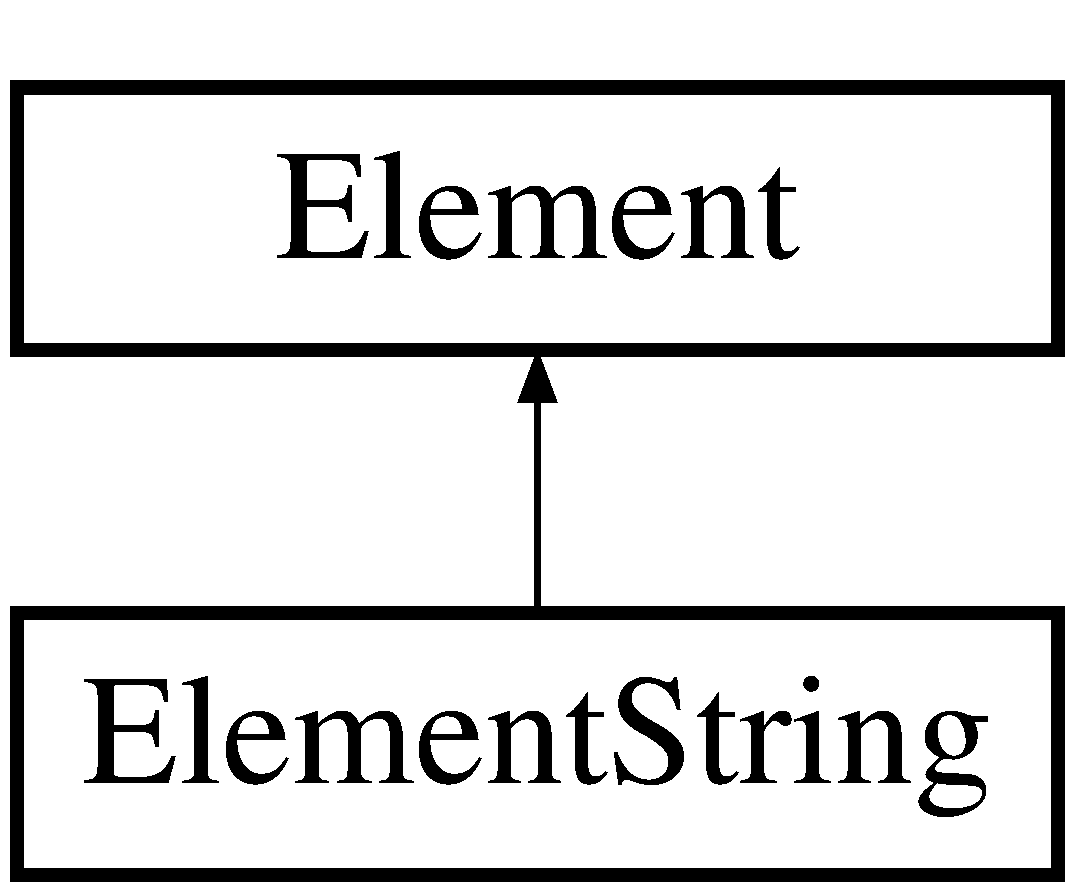
\includegraphics[height=2.000000cm]{classElementString}
\end{center}
\end{figure}
\subsection*{Public Member Functions}
\begin{DoxyCompactItemize}
\item 
void \mbox{\hyperlink{classElementString_a781fe545117610d945772b240f24ac44}{read}} (std\+::string \&text, const \mbox{\hyperlink{classContentReader}{Content\+Reader}} $\ast$parser) override
\end{DoxyCompactItemize}
\subsection*{Public Attributes}
\begin{DoxyCompactItemize}
\item 
std\+::string \mbox{\hyperlink{classElementString_a755b6d208dcea9d496da60102e8f0f81}{value}}
\end{DoxyCompactItemize}


\subsection{Detailed Description}
The string \mbox{\hyperlink{classElement}{Element}} for serialization

\begin{DoxyAuthor}{Author}
Mathieu Lochet 
\end{DoxyAuthor}
\begin{DoxyVersion}{Version}
1 
\end{DoxyVersion}


\subsection{Member Function Documentation}
\mbox{\Hypertarget{classElementString_a781fe545117610d945772b240f24ac44}\label{classElementString_a781fe545117610d945772b240f24ac44}} 
\index{Element\+String@{Element\+String}!read@{read}}
\index{read@{read}!Element\+String@{Element\+String}}
\subsubsection{\texorpdfstring{read()}{read()}}
{\footnotesize\ttfamily void Element\+String\+::read (\begin{DoxyParamCaption}\item[{std\+::string \&}]{text,  }\item[{const \mbox{\hyperlink{classContentReader}{Content\+Reader}} $\ast$}]{reader }\end{DoxyParamCaption})\hspace{0.3cm}{\ttfamily [override]}, {\ttfamily [virtual]}}

Used with polymorphism, lead the readers in the right direction for both text and \mbox{\hyperlink{classElement}{Element}} creation. \begin{DoxySeeAlso}{See also}
\mbox{\hyperlink{classContentReader}{Content\+Reader}}
\end{DoxySeeAlso}

\begin{DoxyParams}{Parameters}
{\em text} & the current used text by the reader \\
\hline
{\em reader} & the current reader used \\
\hline
\end{DoxyParams}


Reimplemented from \mbox{\hyperlink{classElement_ab468bd37a9558f5227837a9236bc9e4b}{Element}}.



\subsection{Member Data Documentation}
\mbox{\Hypertarget{classElementString_a755b6d208dcea9d496da60102e8f0f81}\label{classElementString_a755b6d208dcea9d496da60102e8f0f81}} 
\index{Element\+String@{Element\+String}!value@{value}}
\index{value@{value}!Element\+String@{Element\+String}}
\subsubsection{\texorpdfstring{value}{value}}
{\footnotesize\ttfamily std\+::string Element\+String\+::value}

The string value to be used in serialization 

The documentation for this class was generated from the following files\+:\begin{DoxyCompactItemize}
\item 
block\+\_\+chain/utils/serialization/Element.\+h\item 
block\+\_\+chain/utils/serialization/Element.\+cpp\end{DoxyCompactItemize}

\hypertarget{classEncoding}{}\section{Encoding Class Reference}
\label{classEncoding}\index{Encoding@{Encoding}}


{\ttfamily \#include $<$Encoding.\+h$>$}

\subsection*{Static Public Member Functions}
\begin{DoxyCompactItemize}
\item 
static std\+::string \mbox{\hyperlink{classEncoding_afa3343b66a1a0598b2dc01d74cb81861}{to\+Hexa}} (std\+::string str)
\item 
static std\+::string \mbox{\hyperlink{classEncoding_ada74f7af3be5feeebafe09ede785805a}{from\+Hexa}} (std\+::string str)
\end{DoxyCompactItemize}


\subsection{Detailed Description}
An encoding util. The static class encoding allows to encode any string in hexadecimal and get any text from its hexadecimal form.

\begin{DoxyAuthor}{Author}
Mathieu Lochet 
\end{DoxyAuthor}
\begin{DoxyVersion}{Version}
1 
\end{DoxyVersion}


\subsection{Member Function Documentation}
\mbox{\Hypertarget{classEncoding_ada74f7af3be5feeebafe09ede785805a}\label{classEncoding_ada74f7af3be5feeebafe09ede785805a}} 
\index{Encoding@{Encoding}!from\+Hexa@{from\+Hexa}}
\index{from\+Hexa@{from\+Hexa}!Encoding@{Encoding}}
\subsubsection{\texorpdfstring{from\+Hexa()}{fromHexa()}}
{\footnotesize\ttfamily std\+::string Encoding\+::from\+Hexa (\begin{DoxyParamCaption}\item[{std\+::string}]{str }\end{DoxyParamCaption})\hspace{0.3cm}{\ttfamily [static]}}

Decode a given text from hexadecimal


\begin{DoxyParams}{Parameters}
{\em str} & string to be converted \\
\hline
\end{DoxyParams}
\begin{DoxyReturn}{Returns}
the decoded string 
\end{DoxyReturn}
\mbox{\Hypertarget{classEncoding_afa3343b66a1a0598b2dc01d74cb81861}\label{classEncoding_afa3343b66a1a0598b2dc01d74cb81861}} 
\index{Encoding@{Encoding}!to\+Hexa@{to\+Hexa}}
\index{to\+Hexa@{to\+Hexa}!Encoding@{Encoding}}
\subsubsection{\texorpdfstring{to\+Hexa()}{toHexa()}}
{\footnotesize\ttfamily std\+::string Encoding\+::to\+Hexa (\begin{DoxyParamCaption}\item[{std\+::string}]{str }\end{DoxyParamCaption})\hspace{0.3cm}{\ttfamily [static]}}

Encode a given text in hexadecimal


\begin{DoxyParams}{Parameters}
{\em str} & string to be converted \\
\hline
\end{DoxyParams}
\begin{DoxyReturn}{Returns}
the encoded string 
\end{DoxyReturn}


The documentation for this class was generated from the following files\+:\begin{DoxyCompactItemize}
\item 
block\+\_\+chain/utils/Encoding.\+h\item 
block\+\_\+chain/utils/Encoding.\+cpp\end{DoxyCompactItemize}

\hypertarget{classFactory}{}\section{Factory$<$ V $>$ Class Template Reference}
\label{classFactory}\index{Factory$<$ V $>$@{Factory$<$ V $>$}}


{\ttfamily \#include $<$Factory.\+h$>$}

\subsection*{Public Member Functions}
\begin{DoxyCompactItemize}
\item 
void \mbox{\hyperlink{classFactory_adeaad06fb30141096cc92f98cc3dffa1}{put}} (const char $\ast$key, V value)
\item 
V \mbox{\hyperlink{classFactory_a8a13e5edc3e0c102a1e2fb85047e99d8}{get}} (const char $\ast$key) const
\item 
factory\+\_\+iterator \mbox{\hyperlink{classFactory_a3ea08050cb96078e9d9624de4220d517}{begin}} ()
\item 
factory\+\_\+iterator \mbox{\hyperlink{classFactory_a8b583450f222b426ba2212365f49638f}{end}} ()
\item 
std\+::string \mbox{\hyperlink{classFactory_a3bb49eea6ec1a75fbe7a8c601f27917d}{to\+String}} (const char $\ast$equal, const char $\ast$separator) const
\end{DoxyCompactItemize}


\subsection{Detailed Description}
\subsubsection*{template$<$typename V$>$\newline
class Factory$<$ V $>$}

A factory is a particular type of map. it takes a const char$\ast$ as key and V as values. It does provide higher level manipulation than classical map.

\begin{DoxyAuthor}{Author}
Mathieu Lochet 
\end{DoxyAuthor}
\begin{DoxyVersion}{Version}
1 
\end{DoxyVersion}


\subsection{Member Function Documentation}
\mbox{\Hypertarget{classFactory_a3ea08050cb96078e9d9624de4220d517}\label{classFactory_a3ea08050cb96078e9d9624de4220d517}} 
\index{Factory@{Factory}!begin@{begin}}
\index{begin@{begin}!Factory@{Factory}}
\subsubsection{\texorpdfstring{begin()}{begin()}}
{\footnotesize\ttfamily template$<$typename V$>$ \\
factory\+\_\+iterator \mbox{\hyperlink{classFactory}{Factory}}$<$ V $>$\+::begin (\begin{DoxyParamCaption}{ }\end{DoxyParamCaption})\hspace{0.3cm}{\ttfamily [inline]}}

Get the begin iterator value from the factory.

\begin{DoxyReturn}{Returns}
the begin iterator on the factory 
\end{DoxyReturn}
\mbox{\Hypertarget{classFactory_a8b583450f222b426ba2212365f49638f}\label{classFactory_a8b583450f222b426ba2212365f49638f}} 
\index{Factory@{Factory}!end@{end}}
\index{end@{end}!Factory@{Factory}}
\subsubsection{\texorpdfstring{end()}{end()}}
{\footnotesize\ttfamily template$<$typename V$>$ \\
factory\+\_\+iterator \mbox{\hyperlink{classFactory}{Factory}}$<$ V $>$\+::end (\begin{DoxyParamCaption}{ }\end{DoxyParamCaption})\hspace{0.3cm}{\ttfamily [inline]}}

Get the end iterator value from the factory.

\begin{DoxyReturn}{Returns}
the end iterator on the factory 
\end{DoxyReturn}
\mbox{\Hypertarget{classFactory_a8a13e5edc3e0c102a1e2fb85047e99d8}\label{classFactory_a8a13e5edc3e0c102a1e2fb85047e99d8}} 
\index{Factory@{Factory}!get@{get}}
\index{get@{get}!Factory@{Factory}}
\subsubsection{\texorpdfstring{get()}{get()}}
{\footnotesize\ttfamily template$<$typename V $>$ \\
V \mbox{\hyperlink{classFactory}{Factory}}$<$ V $>$\+::get (\begin{DoxyParamCaption}\item[{const char $\ast$}]{key }\end{DoxyParamCaption}) const}

Get the value from the map.


\begin{DoxyParams}{Parameters}
{\em key} & the key the user provides \\
\hline
\end{DoxyParams}
\begin{DoxyReturn}{Returns}
the value the key represents 
\end{DoxyReturn}
\mbox{\Hypertarget{classFactory_adeaad06fb30141096cc92f98cc3dffa1}\label{classFactory_adeaad06fb30141096cc92f98cc3dffa1}} 
\index{Factory@{Factory}!put@{put}}
\index{put@{put}!Factory@{Factory}}
\subsubsection{\texorpdfstring{put()}{put()}}
{\footnotesize\ttfamily template$<$typename V$>$ \\
void \mbox{\hyperlink{classFactory}{Factory}}$<$ V $>$\+::put (\begin{DoxyParamCaption}\item[{const char $\ast$}]{key,  }\item[{V}]{value }\end{DoxyParamCaption})}

Add a new value in the map


\begin{DoxyParams}{Parameters}
{\em key} & the key of the value \\
\hline
{\em value} & the new value \\
\hline
\end{DoxyParams}
\mbox{\Hypertarget{classFactory_a3bb49eea6ec1a75fbe7a8c601f27917d}\label{classFactory_a3bb49eea6ec1a75fbe7a8c601f27917d}} 
\index{Factory@{Factory}!to\+String@{to\+String}}
\index{to\+String@{to\+String}!Factory@{Factory}}
\subsubsection{\texorpdfstring{to\+String()}{toString()}}
{\footnotesize\ttfamily template$<$typename V$>$ \\
std\+::string \mbox{\hyperlink{classFactory}{Factory}}$<$ V $>$\+::to\+String (\begin{DoxyParamCaption}\item[{const char $\ast$}]{equal,  }\item[{const char $\ast$}]{separator }\end{DoxyParamCaption}) const\hspace{0.3cm}{\ttfamily [inline]}}

Get the visual representation of the factory.

\begin{DoxyReturn}{Returns}
the visual representation of the factory. 
\end{DoxyReturn}


The documentation for this class was generated from the following file\+:\begin{DoxyCompactItemize}
\item 
block\+\_\+chain/utils/Factory.\+h\end{DoxyCompactItemize}

\hypertarget{classHash}{}\section{Hash Class Reference}
\label{classHash}\index{Hash@{Hash}}


{\ttfamily \#include $<$Hash.\+h$>$}

\subsection*{Public Member Functions}
\begin{DoxyCompactItemize}
\item 
\mbox{\hyperlink{classHash_af482880ad75b67a09d2dcb5e86244d80}{Hash}} ()
\item 
\mbox{\hyperlink{classHash_a0e10d81c96b90a36443999a820e29136}{Hash}} (\mbox{\hyperlink{classHash}{Hash}} $\ast$hash1, \mbox{\hyperlink{classHash}{Hash}} $\ast$value)
\item 
\mbox{\hyperlink{classHash_ae324d51c4ee733ef8f7656e6f1afbbd0}{Hash}} (\mbox{\hyperlink{classHash}{Hash}} $\ast$hash1, double value)
\item 
\mbox{\hyperlink{classHash_aa86acb0f09e74c9e6c75adc063539454}{Hash}} (\mbox{\hyperlink{classHash}{Hash}} $\ast$hash1, int value)
\item 
\mbox{\hyperlink{classHash_a523bc61e293e280273dbcd51d6b13905}{Hash}} (\mbox{\hyperlink{classHash}{Hash}} $\ast$hash1, long long int value)
\item 
\mbox{\hyperlink{classHash_af3c5c785c59f0df2549e25a671370452}{Hash}} (\mbox{\hyperlink{classHash}{Hash}} $\ast$hash1, std\+::string value)
\item 
\mbox{\hyperlink{classHash_a529370f2a9baaf470323284364707a88}{Hash}} (std\+::string value)
\item 
\mbox{\hyperlink{classHash_a1d2f0230c2cfe4d6aaab6d9a055faaf5}{Hash}} (const \mbox{\hyperlink{classComponent}{Component}} $\ast$component, const \mbox{\hyperlink{classSerializer}{Serializer}} $\ast$serializer, const char $\ast$encoding)
\item 
std\+::string \mbox{\hyperlink{classHash_ab1c275871d3d81cd38d58dac5c634042}{to\+\_\+string}} () const
\item 
bool \mbox{\hyperlink{classHash_a8aafc6563e964ff47dcbba955b0c28f2}{operator==}} (\mbox{\hyperlink{classHash}{Hash}} const \&h) const
\item 
\mbox{\hyperlink{classElement}{Element}} $\ast$ \mbox{\hyperlink{classHash_a35e01449aedb17a0172837c87986181e}{to\+Element}} ()
\item 
void \mbox{\hyperlink{classHash_a53825b0981f8027244e7bffd84ab2694}{from\+Element}} (\mbox{\hyperlink{classElementObject}{Element\+Object}} $\ast$e, const \mbox{\hyperlink{classSerializer}{Serializer}} $\ast$serializer, const char $\ast$encoding)
\end{DoxyCompactItemize}


\subsection{Detailed Description}
A class for md5 based hash, based on Open\+S\+LL

\begin{DoxyAuthor}{Author}
Mathieu Lochet 
\end{DoxyAuthor}
\begin{DoxyVersion}{Version}
2 
\end{DoxyVersion}


\subsection{Constructor \& Destructor Documentation}
\mbox{\Hypertarget{classHash_af482880ad75b67a09d2dcb5e86244d80}\label{classHash_af482880ad75b67a09d2dcb5e86244d80}} 
\index{Hash@{Hash}!Hash@{Hash}}
\index{Hash@{Hash}!Hash@{Hash}}
\subsubsection{\texorpdfstring{Hash()}{Hash()}\hspace{0.1cm}{\footnotesize\ttfamily [1/8]}}
{\footnotesize\ttfamily Hash\+::\+Hash (\begin{DoxyParamCaption}{ }\end{DoxyParamCaption})\hspace{0.3cm}{\ttfamily [default]}}

A default constructor \mbox{\Hypertarget{classHash_a0e10d81c96b90a36443999a820e29136}\label{classHash_a0e10d81c96b90a36443999a820e29136}} 
\index{Hash@{Hash}!Hash@{Hash}}
\index{Hash@{Hash}!Hash@{Hash}}
\subsubsection{\texorpdfstring{Hash()}{Hash()}\hspace{0.1cm}{\footnotesize\ttfamily [2/8]}}
{\footnotesize\ttfamily Hash\+::\+Hash (\begin{DoxyParamCaption}\item[{\mbox{\hyperlink{classHash}{Hash}} $\ast$}]{hash1,  }\item[{\mbox{\hyperlink{classHash}{Hash}} $\ast$}]{value }\end{DoxyParamCaption})}

A Constructor that hash the two parameters together


\begin{DoxyParams}{Parameters}
{\em hash1} & First element to hash \\
\hline
{\em value} & Second element to hash \\
\hline
\end{DoxyParams}
\mbox{\Hypertarget{classHash_ae324d51c4ee733ef8f7656e6f1afbbd0}\label{classHash_ae324d51c4ee733ef8f7656e6f1afbbd0}} 
\index{Hash@{Hash}!Hash@{Hash}}
\index{Hash@{Hash}!Hash@{Hash}}
\subsubsection{\texorpdfstring{Hash()}{Hash()}\hspace{0.1cm}{\footnotesize\ttfamily [3/8]}}
{\footnotesize\ttfamily Hash\+::\+Hash (\begin{DoxyParamCaption}\item[{\mbox{\hyperlink{classHash}{Hash}} $\ast$}]{hash1,  }\item[{double}]{value }\end{DoxyParamCaption})}

A Constructor that hash the two parameters together


\begin{DoxyParams}{Parameters}
{\em hash1} & First element to hash \\
\hline
{\em value} & Second element to hash \\
\hline
\end{DoxyParams}
\mbox{\Hypertarget{classHash_aa86acb0f09e74c9e6c75adc063539454}\label{classHash_aa86acb0f09e74c9e6c75adc063539454}} 
\index{Hash@{Hash}!Hash@{Hash}}
\index{Hash@{Hash}!Hash@{Hash}}
\subsubsection{\texorpdfstring{Hash()}{Hash()}\hspace{0.1cm}{\footnotesize\ttfamily [4/8]}}
{\footnotesize\ttfamily Hash\+::\+Hash (\begin{DoxyParamCaption}\item[{\mbox{\hyperlink{classHash}{Hash}} $\ast$}]{hash1,  }\item[{int}]{value }\end{DoxyParamCaption})}

A Constructor that hash the two parameters together


\begin{DoxyParams}{Parameters}
{\em hash1} & First element to hash \\
\hline
{\em value} & Second element to hash \\
\hline
\end{DoxyParams}
\mbox{\Hypertarget{classHash_a523bc61e293e280273dbcd51d6b13905}\label{classHash_a523bc61e293e280273dbcd51d6b13905}} 
\index{Hash@{Hash}!Hash@{Hash}}
\index{Hash@{Hash}!Hash@{Hash}}
\subsubsection{\texorpdfstring{Hash()}{Hash()}\hspace{0.1cm}{\footnotesize\ttfamily [5/8]}}
{\footnotesize\ttfamily Hash\+::\+Hash (\begin{DoxyParamCaption}\item[{\mbox{\hyperlink{classHash}{Hash}} $\ast$}]{hash1,  }\item[{long long int}]{value }\end{DoxyParamCaption})}

A Constructor that hash the two parameters together


\begin{DoxyParams}{Parameters}
{\em hash1} & First element to hash \\
\hline
{\em value} & Second element to hash \\
\hline
\end{DoxyParams}
\mbox{\Hypertarget{classHash_af3c5c785c59f0df2549e25a671370452}\label{classHash_af3c5c785c59f0df2549e25a671370452}} 
\index{Hash@{Hash}!Hash@{Hash}}
\index{Hash@{Hash}!Hash@{Hash}}
\subsubsection{\texorpdfstring{Hash()}{Hash()}\hspace{0.1cm}{\footnotesize\ttfamily [6/8]}}
{\footnotesize\ttfamily Hash\+::\+Hash (\begin{DoxyParamCaption}\item[{\mbox{\hyperlink{classHash}{Hash}} $\ast$}]{hash1,  }\item[{std\+::string}]{value }\end{DoxyParamCaption})}

A Constructor that hash the two parameters together


\begin{DoxyParams}{Parameters}
{\em hash1} & First element to hash \\
\hline
{\em value} & Second element to hash \\
\hline
\end{DoxyParams}
\mbox{\Hypertarget{classHash_a529370f2a9baaf470323284364707a88}\label{classHash_a529370f2a9baaf470323284364707a88}} 
\index{Hash@{Hash}!Hash@{Hash}}
\index{Hash@{Hash}!Hash@{Hash}}
\subsubsection{\texorpdfstring{Hash()}{Hash()}\hspace{0.1cm}{\footnotesize\ttfamily [7/8]}}
{\footnotesize\ttfamily Hash\+::\+Hash (\begin{DoxyParamCaption}\item[{std\+::string}]{value }\end{DoxyParamCaption})}

A Constructor that hash a string value


\begin{DoxyParams}{Parameters}
{\em value} & \mbox{\hyperlink{classElement}{Element}} to \mbox{\hyperlink{classHash}{Hash}} \\
\hline
\end{DoxyParams}
\mbox{\Hypertarget{classHash_a1d2f0230c2cfe4d6aaab6d9a055faaf5}\label{classHash_a1d2f0230c2cfe4d6aaab6d9a055faaf5}} 
\index{Hash@{Hash}!Hash@{Hash}}
\index{Hash@{Hash}!Hash@{Hash}}
\subsubsection{\texorpdfstring{Hash()}{Hash()}\hspace{0.1cm}{\footnotesize\ttfamily [8/8]}}
{\footnotesize\ttfamily Hash\+::\+Hash (\begin{DoxyParamCaption}\item[{const \mbox{\hyperlink{classComponent}{Component}} $\ast$}]{component,  }\item[{const \mbox{\hyperlink{classSerializer}{Serializer}} $\ast$}]{serializer,  }\item[{const char $\ast$}]{encoding }\end{DoxyParamCaption})}

Constructor that \mbox{\hyperlink{classHash}{Hash}} a component object


\begin{DoxyParams}{Parameters}
{\em component} & The component to hash \\
\hline
{\em serializer} & The serializer to serialize the component \\
\hline
{\em encoding} & The encoding to serialize the component \\
\hline
\end{DoxyParams}


\subsection{Member Function Documentation}
\mbox{\Hypertarget{classHash_a53825b0981f8027244e7bffd84ab2694}\label{classHash_a53825b0981f8027244e7bffd84ab2694}} 
\index{Hash@{Hash}!from\+Element@{from\+Element}}
\index{from\+Element@{from\+Element}!Hash@{Hash}}
\subsubsection{\texorpdfstring{from\+Element()}{fromElement()}}
{\footnotesize\ttfamily void Hash\+::from\+Element (\begin{DoxyParamCaption}\item[{\mbox{\hyperlink{classElementObject}{Element\+Object}} $\ast$}]{e,  }\item[{const \mbox{\hyperlink{classSerializer}{Serializer}} $\ast$}]{serializer,  }\item[{const char $\ast$}]{encoding }\end{DoxyParamCaption})}

The function used to build the object from its element representation. the object if it is empty \begin{DoxySeeAlso}{See also}
\mbox{\hyperlink{classElementObject}{Element\+Object}} 

\mbox{\hyperlink{classSerializer}{Serializer}}
\end{DoxySeeAlso}

\begin{DoxyParams}{Parameters}
{\em element} & The \mbox{\hyperlink{classElement}{Element}} representation of the object \\
\hline
{\em s} & The serializer (Can be used if serialization of some elements is needed) \\
\hline
{\em encoding} & The encoding that has been used to create the \mbox{\hyperlink{classElement}{Element}} representation of the object (Can be used if serialization of some elements is needed) \\
\hline
\end{DoxyParams}
\mbox{\Hypertarget{classHash_a8aafc6563e964ff47dcbba955b0c28f2}\label{classHash_a8aafc6563e964ff47dcbba955b0c28f2}} 
\index{Hash@{Hash}!operator==@{operator==}}
\index{operator==@{operator==}!Hash@{Hash}}
\subsubsection{\texorpdfstring{operator==()}{operator==()}}
{\footnotesize\ttfamily bool Hash\+::operator== (\begin{DoxyParamCaption}\item[{\mbox{\hyperlink{classHash}{Hash}} const \&}]{h }\end{DoxyParamCaption}) const\hspace{0.3cm}{\ttfamily [inline]}}

Compare two different Hashes


\begin{DoxyParams}{Parameters}
{\em h} & The \mbox{\hyperlink{classHash}{Hash}} to compare to \\
\hline
\end{DoxyParams}
\begin{DoxyReturn}{Returns}
true if both Hashes are the same, false otherwise 
\end{DoxyReturn}
\mbox{\Hypertarget{classHash_ab1c275871d3d81cd38d58dac5c634042}\label{classHash_ab1c275871d3d81cd38d58dac5c634042}} 
\index{Hash@{Hash}!to\+\_\+string@{to\+\_\+string}}
\index{to\+\_\+string@{to\+\_\+string}!Hash@{Hash}}
\subsubsection{\texorpdfstring{to\+\_\+string()}{to\_string()}}
{\footnotesize\ttfamily std\+::string Hash\+::to\+\_\+string (\begin{DoxyParamCaption}{ }\end{DoxyParamCaption}) const}

Get a string representation of the hash

\begin{DoxyReturn}{Returns}
The string representation of the hash 
\end{DoxyReturn}
\mbox{\Hypertarget{classHash_a35e01449aedb17a0172837c87986181e}\label{classHash_a35e01449aedb17a0172837c87986181e}} 
\index{Hash@{Hash}!to\+Element@{to\+Element}}
\index{to\+Element@{to\+Element}!Hash@{Hash}}
\subsubsection{\texorpdfstring{to\+Element()}{toElement()}}
{\footnotesize\ttfamily \mbox{\hyperlink{classElement}{Element}} $\ast$ Hash\+::to\+Element (\begin{DoxyParamCaption}{ }\end{DoxyParamCaption})}

The method used by the serializer to transform an object into an \mbox{\hyperlink{classElement}{Element}} representation. \begin{DoxySeeAlso}{See also}
\mbox{\hyperlink{classElement}{Element}}
\end{DoxySeeAlso}
\begin{DoxyReturn}{Returns}
The \mbox{\hyperlink{classElement}{Element}} representation of the object 
\end{DoxyReturn}


The documentation for this class was generated from the following files\+:\begin{DoxyCompactItemize}
\item 
block\+\_\+chain/algorithm/Hash.\+h\item 
block\+\_\+chain/algorithm/Hash.\+cpp\end{DoxyCompactItemize}

\hypertarget{classJsonCreator}{}\section{Json\+Creator Class Reference}
\label{classJsonCreator}\index{Json\+Creator@{Json\+Creator}}


{\ttfamily \#include $<$Json\+Creator.\+h$>$}

Inheritance diagram for Json\+Creator\+:\begin{figure}[H]
\begin{center}
\leavevmode
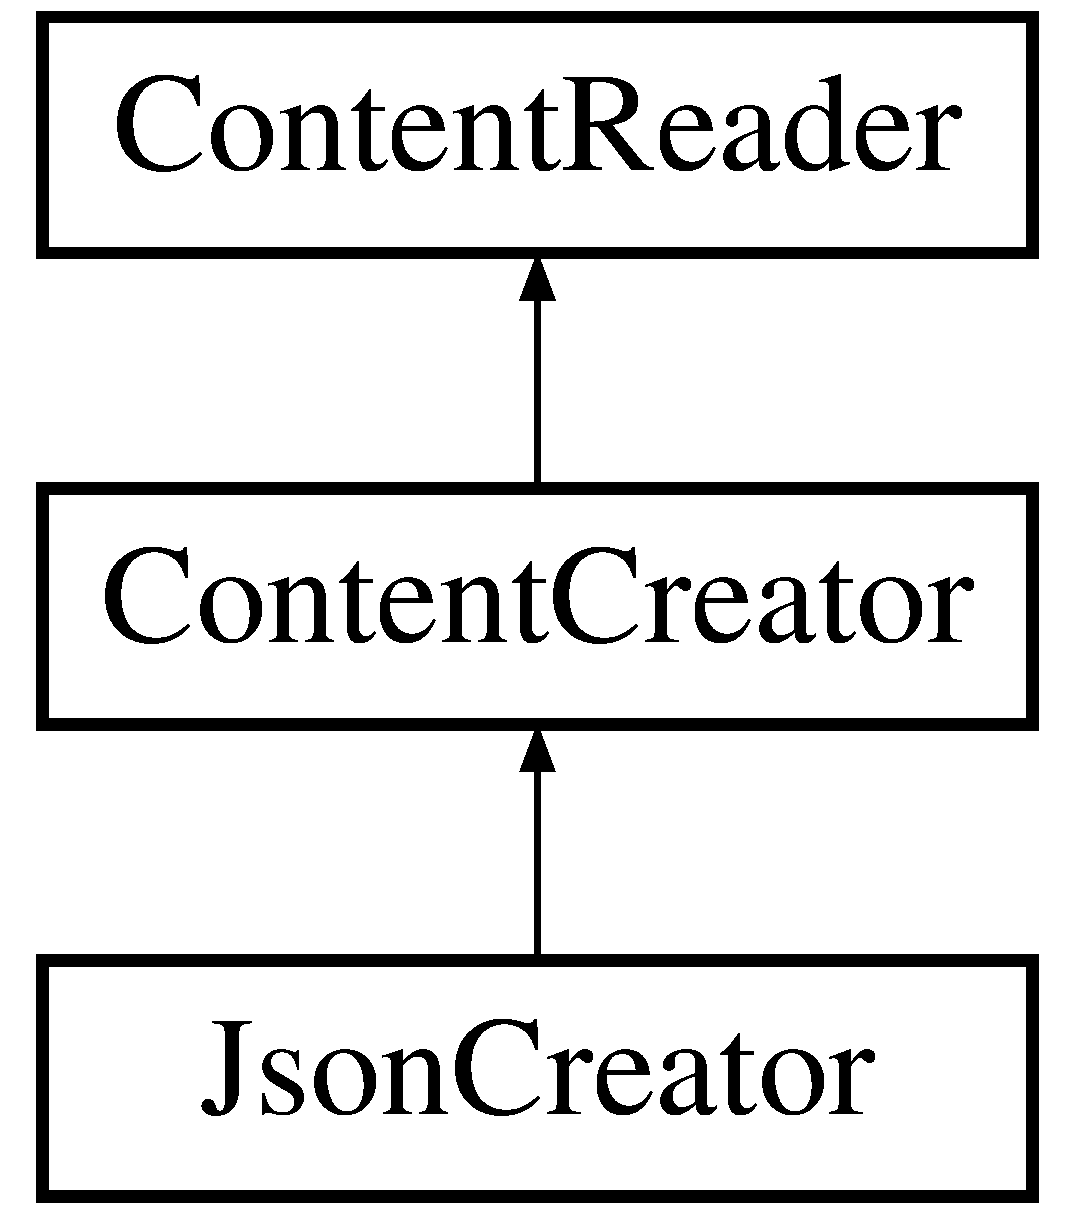
\includegraphics[height=3.000000cm]{classJsonCreator}
\end{center}
\end{figure}
\subsection*{Public Member Functions}
\begin{DoxyCompactItemize}
\item 
void \mbox{\hyperlink{classJsonCreator_a505ff309c6b144d29478804b0e187c6f}{parse}} (std\+::string \&text, \mbox{\hyperlink{classElement}{Element}} $\ast$$\ast$e) const override
\item 
void \mbox{\hyperlink{classJsonCreator_a0fe34794ee3563c3e0bc35006129fcdc}{parse\+Content}} (std\+::string \&text, \mbox{\hyperlink{classElementInt}{Element\+Int}} $\ast$e) const override
\item 
void \mbox{\hyperlink{classJsonCreator_acf8d7cd3dcbb669fd9eb5dec95e069f3}{parse\+Content}} (std\+::string \&text, \mbox{\hyperlink{classElementString}{Element\+String}} $\ast$e) const override
\item 
void \mbox{\hyperlink{classJsonCreator_a95fb65046a7467b8e48feaf92a62b40c}{parse\+Content}} (std\+::string \&text, \mbox{\hyperlink{classElementBoolean}{Element\+Boolean}} $\ast$e) const override
\item 
void \mbox{\hyperlink{classJsonCreator_a694669d359eb73890a9e9f247c4ebab4}{parse\+Content}} (std\+::string \&text, \mbox{\hyperlink{classElementArray}{Element\+Array}} $\ast$e) const override
\item 
void \mbox{\hyperlink{classJsonCreator_a9f57af1a7925074b8e3e4175f74c886a}{parse\+Content}} (std\+::string \&text, \mbox{\hyperlink{classElementObject}{Element\+Object}} $\ast$e) const override
\item 
void \mbox{\hyperlink{classJsonCreator_a5e841806165fd5cb595d9f7d7c924080}{parse\+Content}} (std\+::string \&text, \mbox{\hyperlink{classElementDouble}{Element\+Double}} $\ast$e) const override
\item 
const char $\ast$ \mbox{\hyperlink{classJsonCreator_ab7313de0040d40a26a9386eb3714120c}{get\+\_\+encoding}} () const override
\item 
\mbox{\hyperlink{classJsonCreator_a71197e5dafee7dd9c04c208413050860}{Json\+Creator}} ()
\item 
\mbox{\hyperlink{classJsonCreator_a061eaa469894ab51ae6c046016da9e40}{$\sim$\+Json\+Creator}} ()
\end{DoxyCompactItemize}


\subsection{Detailed Description}
A creator conceived to create any json file for given Elements \begin{DoxySeeAlso}{See also}
\mbox{\hyperlink{classContentCreator}{Content\+Creator}} 

\mbox{\hyperlink{classElement}{Element}}
\end{DoxySeeAlso}
\begin{DoxyAuthor}{Author}
Mathieu Lochet 
\end{DoxyAuthor}
\begin{DoxyVersion}{Version}
1 
\end{DoxyVersion}


\subsection{Constructor \& Destructor Documentation}
\mbox{\Hypertarget{classJsonCreator_a71197e5dafee7dd9c04c208413050860}\label{classJsonCreator_a71197e5dafee7dd9c04c208413050860}} 
\index{Json\+Creator@{Json\+Creator}!Json\+Creator@{Json\+Creator}}
\index{Json\+Creator@{Json\+Creator}!Json\+Creator@{Json\+Creator}}
\subsubsection{\texorpdfstring{Json\+Creator()}{JsonCreator()}}
{\footnotesize\ttfamily Json\+Creator\+::\+Json\+Creator (\begin{DoxyParamCaption}{ }\end{DoxyParamCaption})\hspace{0.3cm}{\ttfamily [default]}}

Default constructor \mbox{\Hypertarget{classJsonCreator_a061eaa469894ab51ae6c046016da9e40}\label{classJsonCreator_a061eaa469894ab51ae6c046016da9e40}} 
\index{Json\+Creator@{Json\+Creator}!````~Json\+Creator@{$\sim$\+Json\+Creator}}
\index{````~Json\+Creator@{$\sim$\+Json\+Creator}!Json\+Creator@{Json\+Creator}}
\subsubsection{\texorpdfstring{$\sim$\+Json\+Creator()}{~JsonCreator()}}
{\footnotesize\ttfamily Json\+Creator\+::$\sim$\+Json\+Creator (\begin{DoxyParamCaption}{ }\end{DoxyParamCaption})\hspace{0.3cm}{\ttfamily [default]}}

Default destructor 

\subsection{Member Function Documentation}
\mbox{\Hypertarget{classJsonCreator_ab7313de0040d40a26a9386eb3714120c}\label{classJsonCreator_ab7313de0040d40a26a9386eb3714120c}} 
\index{Json\+Creator@{Json\+Creator}!get\+\_\+encoding@{get\+\_\+encoding}}
\index{get\+\_\+encoding@{get\+\_\+encoding}!Json\+Creator@{Json\+Creator}}
\subsubsection{\texorpdfstring{get\+\_\+encoding()}{get\_encoding()}}
{\footnotesize\ttfamily const char $\ast$ Json\+Creator\+::get\+\_\+encoding (\begin{DoxyParamCaption}{ }\end{DoxyParamCaption}) const\hspace{0.3cm}{\ttfamily [override]}, {\ttfamily [virtual]}}

Get the encoding corresponding to the reader

\begin{DoxyReturn}{Returns}
The corresponding encoding for serialization 
\end{DoxyReturn}


Implements \mbox{\hyperlink{classContentReader_a1495a4402c4fac02d8cd2542b61c6eed}{Content\+Reader}}.

\mbox{\Hypertarget{classJsonCreator_a505ff309c6b144d29478804b0e187c6f}\label{classJsonCreator_a505ff309c6b144d29478804b0e187c6f}} 
\index{Json\+Creator@{Json\+Creator}!parse@{parse}}
\index{parse@{parse}!Json\+Creator@{Json\+Creator}}
\subsubsection{\texorpdfstring{parse()}{parse()}}
{\footnotesize\ttfamily void Json\+Creator\+::parse (\begin{DoxyParamCaption}\item[{std\+::string \&}]{text,  }\item[{\mbox{\hyperlink{classElement}{Element}} $\ast$$\ast$}]{e }\end{DoxyParamCaption}) const\hspace{0.3cm}{\ttfamily [override]}, {\ttfamily [virtual]}}

The entry point of the parser\+: it reads the text and generates the first element according to rules. Calls the corresponding methods for recursive parsing. (opposite works as well) \begin{DoxySeeAlso}{See also}
\mbox{\hyperlink{classJsonCreator_a0fe34794ee3563c3e0bc35006129fcdc}{parse\+Content}} 

\mbox{\hyperlink{classElement}{Element}}
\end{DoxySeeAlso}

\begin{DoxyParams}{Parameters}
{\em text} & a given text \\
\hline
{\em e} & the root \mbox{\hyperlink{classElement}{Element}} that will be generated (or used) \\
\hline
\end{DoxyParams}


Implements \mbox{\hyperlink{classContentReader_a7fff2e63a2e8fa216665604f69974e1d}{Content\+Reader}}.

\mbox{\Hypertarget{classJsonCreator_a0fe34794ee3563c3e0bc35006129fcdc}\label{classJsonCreator_a0fe34794ee3563c3e0bc35006129fcdc}} 
\index{Json\+Creator@{Json\+Creator}!parse\+Content@{parse\+Content}}
\index{parse\+Content@{parse\+Content}!Json\+Creator@{Json\+Creator}}
\subsubsection{\texorpdfstring{parse\+Content()}{parseContent()}\hspace{0.1cm}{\footnotesize\ttfamily [1/6]}}
{\footnotesize\ttfamily void Json\+Creator\+::parse\+Content (\begin{DoxyParamCaption}\item[{std\+::string \&}]{text,  }\item[{\mbox{\hyperlink{classElementInt}{Element\+Int}} $\ast$}]{e }\end{DoxyParamCaption}) const\hspace{0.3cm}{\ttfamily [override]}, {\ttfamily [virtual]}}

Generates an integer from a given string. Calls the method parse with the rest of the string. (opposite works as well) \begin{DoxySeeAlso}{See also}
\mbox{\hyperlink{classJsonCreator_a505ff309c6b144d29478804b0e187c6f}{parse}} 

\mbox{\hyperlink{classElementInt}{Element\+Int}}
\end{DoxySeeAlso}

\begin{DoxyParams}{Parameters}
{\em text} & a given text \\
\hline
{\em e} & the int \mbox{\hyperlink{classElement}{Element}} that will be generated (or used) \\
\hline
\end{DoxyParams}


Implements \mbox{\hyperlink{classContentReader_a7eef37b8b9761e21c0a3907ff94c72f7}{Content\+Reader}}.

\mbox{\Hypertarget{classJsonCreator_acf8d7cd3dcbb669fd9eb5dec95e069f3}\label{classJsonCreator_acf8d7cd3dcbb669fd9eb5dec95e069f3}} 
\index{Json\+Creator@{Json\+Creator}!parse\+Content@{parse\+Content}}
\index{parse\+Content@{parse\+Content}!Json\+Creator@{Json\+Creator}}
\subsubsection{\texorpdfstring{parse\+Content()}{parseContent()}\hspace{0.1cm}{\footnotesize\ttfamily [2/6]}}
{\footnotesize\ttfamily void Json\+Creator\+::parse\+Content (\begin{DoxyParamCaption}\item[{std\+::string \&}]{text,  }\item[{\mbox{\hyperlink{classElementString}{Element\+String}} $\ast$}]{e }\end{DoxyParamCaption}) const\hspace{0.3cm}{\ttfamily [override]}, {\ttfamily [virtual]}}

Generates an string from a given string. it stops with the defined rules of the parser. Calls the method parse with the rest of the string. (opposite works as well) \begin{DoxySeeAlso}{See also}
\mbox{\hyperlink{classJsonCreator_a505ff309c6b144d29478804b0e187c6f}{parse}} 

\mbox{\hyperlink{classElementString}{Element\+String}}
\end{DoxySeeAlso}

\begin{DoxyParams}{Parameters}
{\em text} & a given text \\
\hline
{\em e} & the string \mbox{\hyperlink{classElement}{Element}} that will be generated (or used) \\
\hline
\end{DoxyParams}


Implements \mbox{\hyperlink{classContentReader_a310678ddc37a05aca2f13db73b22abe5}{Content\+Reader}}.

\mbox{\Hypertarget{classJsonCreator_a95fb65046a7467b8e48feaf92a62b40c}\label{classJsonCreator_a95fb65046a7467b8e48feaf92a62b40c}} 
\index{Json\+Creator@{Json\+Creator}!parse\+Content@{parse\+Content}}
\index{parse\+Content@{parse\+Content}!Json\+Creator@{Json\+Creator}}
\subsubsection{\texorpdfstring{parse\+Content()}{parseContent()}\hspace{0.1cm}{\footnotesize\ttfamily [3/6]}}
{\footnotesize\ttfamily void Json\+Creator\+::parse\+Content (\begin{DoxyParamCaption}\item[{std\+::string \&}]{text,  }\item[{\mbox{\hyperlink{classElementBoolean}{Element\+Boolean}} $\ast$}]{e }\end{DoxyParamCaption}) const\hspace{0.3cm}{\ttfamily [override]}, {\ttfamily [virtual]}}

Generates an boolean from a given string. Calls the method parse with the rest of the string. (opposite works as well) \begin{DoxySeeAlso}{See also}
\mbox{\hyperlink{classJsonCreator_a505ff309c6b144d29478804b0e187c6f}{parse}} 

\mbox{\hyperlink{classElementBoolean}{Element\+Boolean}}
\end{DoxySeeAlso}

\begin{DoxyParams}{Parameters}
{\em text} & a given text \\
\hline
{\em e} & the boolean \mbox{\hyperlink{classElement}{Element}} that will be generated (or used) \\
\hline
\end{DoxyParams}


Implements \mbox{\hyperlink{classContentReader_a3ee0aec579c723f17742e10fe7c75e39}{Content\+Reader}}.

\mbox{\Hypertarget{classJsonCreator_a694669d359eb73890a9e9f247c4ebab4}\label{classJsonCreator_a694669d359eb73890a9e9f247c4ebab4}} 
\index{Json\+Creator@{Json\+Creator}!parse\+Content@{parse\+Content}}
\index{parse\+Content@{parse\+Content}!Json\+Creator@{Json\+Creator}}
\subsubsection{\texorpdfstring{parse\+Content()}{parseContent()}\hspace{0.1cm}{\footnotesize\ttfamily [4/6]}}
{\footnotesize\ttfamily void Json\+Creator\+::parse\+Content (\begin{DoxyParamCaption}\item[{std\+::string \&}]{text,  }\item[{\mbox{\hyperlink{classElementArray}{Element\+Array}} $\ast$}]{e }\end{DoxyParamCaption}) const\hspace{0.3cm}{\ttfamily [override]}, {\ttfamily [virtual]}}

Generates an array of Elements from a given string. Calls the method parse with the rest of the string and parse each of the found elements of the array. (opposite works as well) \begin{DoxySeeAlso}{See also}
\mbox{\hyperlink{classJsonCreator_a505ff309c6b144d29478804b0e187c6f}{parse}} 

\mbox{\hyperlink{classElement}{Element}} 

\mbox{\hyperlink{classElementArray}{Element\+Array}}
\end{DoxySeeAlso}

\begin{DoxyParams}{Parameters}
{\em text} & a given text \\
\hline
{\em e} & the array \mbox{\hyperlink{classElement}{Element}} that will be generated (or used) \\
\hline
\end{DoxyParams}


Implements \mbox{\hyperlink{classContentReader_a91fdd738983dcc7a246c3c163007dfa9}{Content\+Reader}}.

\mbox{\Hypertarget{classJsonCreator_a9f57af1a7925074b8e3e4175f74c886a}\label{classJsonCreator_a9f57af1a7925074b8e3e4175f74c886a}} 
\index{Json\+Creator@{Json\+Creator}!parse\+Content@{parse\+Content}}
\index{parse\+Content@{parse\+Content}!Json\+Creator@{Json\+Creator}}
\subsubsection{\texorpdfstring{parse\+Content()}{parseContent()}\hspace{0.1cm}{\footnotesize\ttfamily [5/6]}}
{\footnotesize\ttfamily void Json\+Creator\+::parse\+Content (\begin{DoxyParamCaption}\item[{std\+::string \&}]{text,  }\item[{\mbox{\hyperlink{classElementObject}{Element\+Object}} $\ast$}]{e }\end{DoxyParamCaption}) const\hspace{0.3cm}{\ttfamily [override]}, {\ttfamily [virtual]}}

Generates an object of $<$key (string), Elements$>$ from a given string. Calls the method parse with the rest of the string and parse each of the found elements of the object. (opposite works as well) \begin{DoxySeeAlso}{See also}
\mbox{\hyperlink{classJsonCreator_a505ff309c6b144d29478804b0e187c6f}{parse}} 

\mbox{\hyperlink{classElement}{Element}} 

\mbox{\hyperlink{classElementObject}{Element\+Object}}
\end{DoxySeeAlso}

\begin{DoxyParams}{Parameters}
{\em text} & a given text \\
\hline
{\em e} & the object \mbox{\hyperlink{classElement}{Element}} that will be generated (or used) \\
\hline
\end{DoxyParams}


Implements \mbox{\hyperlink{classContentReader_a59a8de2bf3436e46b4d029a9b3c3c9da}{Content\+Reader}}.

\mbox{\Hypertarget{classJsonCreator_a5e841806165fd5cb595d9f7d7c924080}\label{classJsonCreator_a5e841806165fd5cb595d9f7d7c924080}} 
\index{Json\+Creator@{Json\+Creator}!parse\+Content@{parse\+Content}}
\index{parse\+Content@{parse\+Content}!Json\+Creator@{Json\+Creator}}
\subsubsection{\texorpdfstring{parse\+Content()}{parseContent()}\hspace{0.1cm}{\footnotesize\ttfamily [6/6]}}
{\footnotesize\ttfamily void Json\+Creator\+::parse\+Content (\begin{DoxyParamCaption}\item[{std\+::string \&}]{text,  }\item[{\mbox{\hyperlink{classElementDouble}{Element\+Double}} $\ast$}]{e }\end{DoxyParamCaption}) const\hspace{0.3cm}{\ttfamily [override]}, {\ttfamily [virtual]}}

Generates an double from a given string. Calls the method parse with the rest of the string. (opposite works as well) \begin{DoxySeeAlso}{See also}
\mbox{\hyperlink{classJsonCreator_a505ff309c6b144d29478804b0e187c6f}{parse}} 

\mbox{\hyperlink{classElementDouble}{Element\+Double}}
\end{DoxySeeAlso}

\begin{DoxyParams}{Parameters}
{\em text} & a given text \\
\hline
{\em e} & the double \mbox{\hyperlink{classElement}{Element}} that will be generated (or used) \\
\hline
\end{DoxyParams}


Implements \mbox{\hyperlink{classContentReader_ab4ba739ee5241848ae8af86e64e43a40}{Content\+Reader}}.



The documentation for this class was generated from the following files\+:\begin{DoxyCompactItemize}
\item 
block\+\_\+chain/utils/serialization/json/Json\+Creator.\+h\item 
block\+\_\+chain/utils/serialization/json/Json\+Creator.\+cpp\end{DoxyCompactItemize}

\hypertarget{classJsonParser}{}\section{Json\+Parser Class Reference}
\label{classJsonParser}\index{Json\+Parser@{Json\+Parser}}


{\ttfamily \#include $<$Json\+Parser.\+h$>$}

Inheritance diagram for Json\+Parser\+:\begin{figure}[H]
\begin{center}
\leavevmode
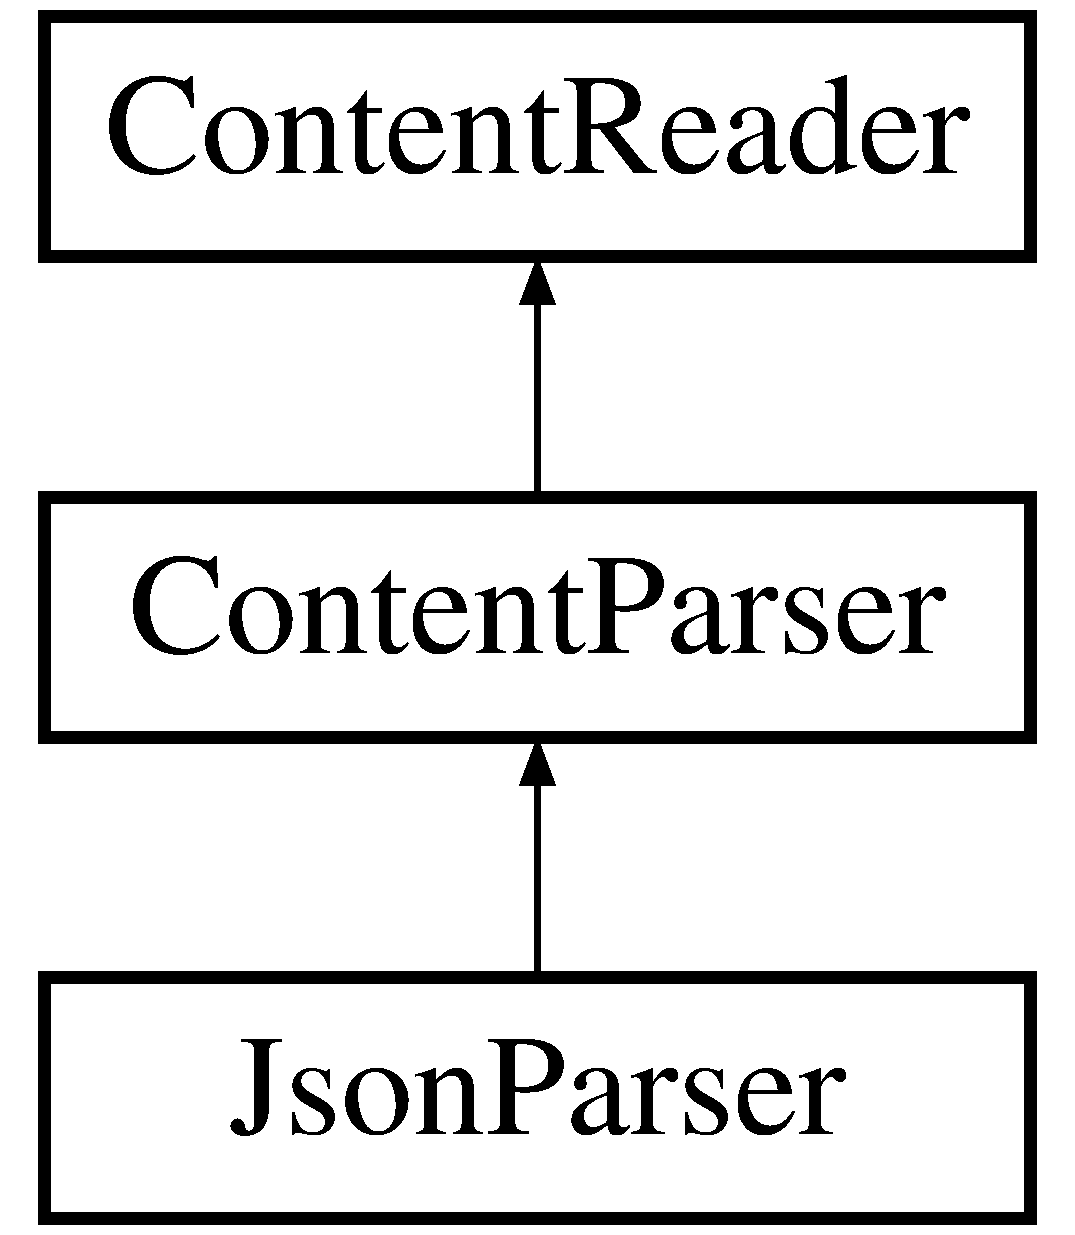
\includegraphics[height=3.000000cm]{classJsonParser}
\end{center}
\end{figure}
\subsection*{Public Member Functions}
\begin{DoxyCompactItemize}
\item 
void \mbox{\hyperlink{classJsonParser_a3ec3a9fcc8a63f987b4749d60b0568df}{parse}} (std\+::string \&text, \mbox{\hyperlink{classElement}{Element}} $\ast$$\ast$e) const override
\item 
void \mbox{\hyperlink{classJsonParser_ac80cf84ff2565f4c1f3a0f5ddb559c96}{parse\+Content}} (std\+::string \&text, \mbox{\hyperlink{classElementInt}{Element\+Int}} $\ast$e) const override
\item 
void \mbox{\hyperlink{classJsonParser_a94737a7518f05e4ed43a753f4148b354}{parse\+Content}} (std\+::string \&text, \mbox{\hyperlink{classElementString}{Element\+String}} $\ast$e) const override
\item 
void \mbox{\hyperlink{classJsonParser_a0857f5d286e5f0b973e2791e5e7a4e83}{parse\+Content}} (std\+::string \&text, \mbox{\hyperlink{classElementBoolean}{Element\+Boolean}} $\ast$e) const override
\item 
void \mbox{\hyperlink{classJsonParser_aa728c443b247b83cdf6cedb406d8940d}{parse\+Content}} (std\+::string \&text, \mbox{\hyperlink{classElementArray}{Element\+Array}} $\ast$e) const override
\item 
void \mbox{\hyperlink{classJsonParser_a7d4fad0f0947a74ca158dc1922c97355}{parse\+Content}} (std\+::string \&text, \mbox{\hyperlink{classElementObject}{Element\+Object}} $\ast$e) const override
\item 
void \mbox{\hyperlink{classJsonParser_a07a4f2b10547d5f2251bc1f7b09d02c1}{parse\+Content}} (std\+::string \&text, \mbox{\hyperlink{classElementDouble}{Element\+Double}} $\ast$e) const override
\item 
\mbox{\hyperlink{classJsonParser_af21abdfb0ceac731e44d897a0285f5d4}{Json\+Parser}} ()
\item 
\mbox{\hyperlink{classJsonParser_a7c0393b54c37f9ff30b6bb59f0ba92ce}{$\sim$\+Json\+Parser}} ()
\end{DoxyCompactItemize}


\subsection{Detailed Description}
A parser conceived to parse any json file in an \mbox{\hyperlink{classElement}{Element}} representation \begin{DoxySeeAlso}{See also}
\mbox{\hyperlink{classContentParser}{Content\+Parser}} 

\mbox{\hyperlink{classElement}{Element}}
\end{DoxySeeAlso}
\begin{DoxyAuthor}{Author}
Mathieu Lochet 
\end{DoxyAuthor}
\begin{DoxyVersion}{Version}
1 
\end{DoxyVersion}


\subsection{Constructor \& Destructor Documentation}
\mbox{\Hypertarget{classJsonParser_af21abdfb0ceac731e44d897a0285f5d4}\label{classJsonParser_af21abdfb0ceac731e44d897a0285f5d4}} 
\index{Json\+Parser@{Json\+Parser}!Json\+Parser@{Json\+Parser}}
\index{Json\+Parser@{Json\+Parser}!Json\+Parser@{Json\+Parser}}
\subsubsection{\texorpdfstring{Json\+Parser()}{JsonParser()}}
{\footnotesize\ttfamily Json\+Parser\+::\+Json\+Parser (\begin{DoxyParamCaption}{ }\end{DoxyParamCaption})}

The parser constructor\+: initialize the map of different possible elements \mbox{\Hypertarget{classJsonParser_a7c0393b54c37f9ff30b6bb59f0ba92ce}\label{classJsonParser_a7c0393b54c37f9ff30b6bb59f0ba92ce}} 
\index{Json\+Parser@{Json\+Parser}!````~Json\+Parser@{$\sim$\+Json\+Parser}}
\index{````~Json\+Parser@{$\sim$\+Json\+Parser}!Json\+Parser@{Json\+Parser}}
\subsubsection{\texorpdfstring{$\sim$\+Json\+Parser()}{~JsonParser()}}
{\footnotesize\ttfamily Json\+Parser\+::$\sim$\+Json\+Parser (\begin{DoxyParamCaption}{ }\end{DoxyParamCaption})\hspace{0.3cm}{\ttfamily [default]}}

The parser destructor\+: frees the map of elements 

\subsection{Member Function Documentation}
\mbox{\Hypertarget{classJsonParser_a3ec3a9fcc8a63f987b4749d60b0568df}\label{classJsonParser_a3ec3a9fcc8a63f987b4749d60b0568df}} 
\index{Json\+Parser@{Json\+Parser}!parse@{parse}}
\index{parse@{parse}!Json\+Parser@{Json\+Parser}}
\subsubsection{\texorpdfstring{parse()}{parse()}}
{\footnotesize\ttfamily void Json\+Parser\+::parse (\begin{DoxyParamCaption}\item[{std\+::string \&}]{text,  }\item[{\mbox{\hyperlink{classElement}{Element}} $\ast$$\ast$}]{e }\end{DoxyParamCaption}) const\hspace{0.3cm}{\ttfamily [override]}, {\ttfamily [virtual]}}

The entry point of the parser\+: it reads the text and generate the first element according to rules. Calls the corresponding methods for recursive parsing. (opposite works as well) \begin{DoxySeeAlso}{See also}
\mbox{\hyperlink{classJsonParser_ac80cf84ff2565f4c1f3a0f5ddb559c96}{parse\+Content}} 

\mbox{\hyperlink{classElement}{Element}}
\end{DoxySeeAlso}

\begin{DoxyParams}{Parameters}
{\em text} & a given text \\
\hline
{\em e} & the root \mbox{\hyperlink{classElement}{Element}} that will be generated (or used) \\
\hline
\end{DoxyParams}


Implements \mbox{\hyperlink{classContentReader_a7fff2e63a2e8fa216665604f69974e1d}{Content\+Reader}}.

\mbox{\Hypertarget{classJsonParser_ac80cf84ff2565f4c1f3a0f5ddb559c96}\label{classJsonParser_ac80cf84ff2565f4c1f3a0f5ddb559c96}} 
\index{Json\+Parser@{Json\+Parser}!parse\+Content@{parse\+Content}}
\index{parse\+Content@{parse\+Content}!Json\+Parser@{Json\+Parser}}
\subsubsection{\texorpdfstring{parse\+Content()}{parseContent()}\hspace{0.1cm}{\footnotesize\ttfamily [1/6]}}
{\footnotesize\ttfamily void Json\+Parser\+::parse\+Content (\begin{DoxyParamCaption}\item[{std\+::string \&}]{text,  }\item[{\mbox{\hyperlink{classElementInt}{Element\+Int}} $\ast$}]{e }\end{DoxyParamCaption}) const\hspace{0.3cm}{\ttfamily [override]}, {\ttfamily [virtual]}}

Generates an integer from a given string. Calls the method parse with the rest of the string. (opposite works as well) \begin{DoxySeeAlso}{See also}
\mbox{\hyperlink{classJsonParser_a3ec3a9fcc8a63f987b4749d60b0568df}{parse}} 

\mbox{\hyperlink{classElementInt}{Element\+Int}}
\end{DoxySeeAlso}

\begin{DoxyParams}{Parameters}
{\em text} & a given text \\
\hline
{\em e} & the int \mbox{\hyperlink{classElement}{Element}} that will be generated (or used) \\
\hline
\end{DoxyParams}


Implements \mbox{\hyperlink{classContentReader_a7eef37b8b9761e21c0a3907ff94c72f7}{Content\+Reader}}.

\mbox{\Hypertarget{classJsonParser_a94737a7518f05e4ed43a753f4148b354}\label{classJsonParser_a94737a7518f05e4ed43a753f4148b354}} 
\index{Json\+Parser@{Json\+Parser}!parse\+Content@{parse\+Content}}
\index{parse\+Content@{parse\+Content}!Json\+Parser@{Json\+Parser}}
\subsubsection{\texorpdfstring{parse\+Content()}{parseContent()}\hspace{0.1cm}{\footnotesize\ttfamily [2/6]}}
{\footnotesize\ttfamily void Json\+Parser\+::parse\+Content (\begin{DoxyParamCaption}\item[{std\+::string \&}]{text,  }\item[{\mbox{\hyperlink{classElementString}{Element\+String}} $\ast$}]{e }\end{DoxyParamCaption}) const\hspace{0.3cm}{\ttfamily [override]}, {\ttfamily [virtual]}}

Generates an string from a given string. it stops with the defined rules of the parser. Calls the method parse with the rest of the string. (opposite works as well) \begin{DoxySeeAlso}{See also}
\mbox{\hyperlink{classJsonParser_a3ec3a9fcc8a63f987b4749d60b0568df}{parse}} 

\mbox{\hyperlink{classElementString}{Element\+String}}
\end{DoxySeeAlso}

\begin{DoxyParams}{Parameters}
{\em text} & a given text \\
\hline
{\em e} & the string \mbox{\hyperlink{classElement}{Element}} that will be generated (or used) \\
\hline
\end{DoxyParams}


Implements \mbox{\hyperlink{classContentReader_a310678ddc37a05aca2f13db73b22abe5}{Content\+Reader}}.

\mbox{\Hypertarget{classJsonParser_a0857f5d286e5f0b973e2791e5e7a4e83}\label{classJsonParser_a0857f5d286e5f0b973e2791e5e7a4e83}} 
\index{Json\+Parser@{Json\+Parser}!parse\+Content@{parse\+Content}}
\index{parse\+Content@{parse\+Content}!Json\+Parser@{Json\+Parser}}
\subsubsection{\texorpdfstring{parse\+Content()}{parseContent()}\hspace{0.1cm}{\footnotesize\ttfamily [3/6]}}
{\footnotesize\ttfamily void Json\+Parser\+::parse\+Content (\begin{DoxyParamCaption}\item[{std\+::string \&}]{text,  }\item[{\mbox{\hyperlink{classElementBoolean}{Element\+Boolean}} $\ast$}]{e }\end{DoxyParamCaption}) const\hspace{0.3cm}{\ttfamily [override]}, {\ttfamily [virtual]}}

Generates an boolean from a given string. Calls the method parse with the rest of the string. (opposite works as well) \begin{DoxySeeAlso}{See also}
\mbox{\hyperlink{classJsonParser_a3ec3a9fcc8a63f987b4749d60b0568df}{parse}} 

\mbox{\hyperlink{classElementBoolean}{Element\+Boolean}}
\end{DoxySeeAlso}

\begin{DoxyParams}{Parameters}
{\em text} & a given text \\
\hline
{\em e} & the boolean \mbox{\hyperlink{classElement}{Element}} that will be generated (or used) \\
\hline
\end{DoxyParams}


Implements \mbox{\hyperlink{classContentReader_a3ee0aec579c723f17742e10fe7c75e39}{Content\+Reader}}.

\mbox{\Hypertarget{classJsonParser_aa728c443b247b83cdf6cedb406d8940d}\label{classJsonParser_aa728c443b247b83cdf6cedb406d8940d}} 
\index{Json\+Parser@{Json\+Parser}!parse\+Content@{parse\+Content}}
\index{parse\+Content@{parse\+Content}!Json\+Parser@{Json\+Parser}}
\subsubsection{\texorpdfstring{parse\+Content()}{parseContent()}\hspace{0.1cm}{\footnotesize\ttfamily [4/6]}}
{\footnotesize\ttfamily void Json\+Parser\+::parse\+Content (\begin{DoxyParamCaption}\item[{std\+::string \&}]{text,  }\item[{\mbox{\hyperlink{classElementArray}{Element\+Array}} $\ast$}]{e }\end{DoxyParamCaption}) const\hspace{0.3cm}{\ttfamily [override]}, {\ttfamily [virtual]}}

Generates an array of Elements from a given string. Calls the method parse with the rest of the string and parse each of the found elements of the array. (opposite works as well) \begin{DoxySeeAlso}{See also}
\mbox{\hyperlink{classJsonParser_a3ec3a9fcc8a63f987b4749d60b0568df}{parse}} 

\mbox{\hyperlink{classElement}{Element}} 

\mbox{\hyperlink{classElementArray}{Element\+Array}}
\end{DoxySeeAlso}

\begin{DoxyParams}{Parameters}
{\em text} & a given text \\
\hline
{\em e} & the array \mbox{\hyperlink{classElement}{Element}} that will be generated (or used) \\
\hline
\end{DoxyParams}


Implements \mbox{\hyperlink{classContentReader_a91fdd738983dcc7a246c3c163007dfa9}{Content\+Reader}}.

\mbox{\Hypertarget{classJsonParser_a7d4fad0f0947a74ca158dc1922c97355}\label{classJsonParser_a7d4fad0f0947a74ca158dc1922c97355}} 
\index{Json\+Parser@{Json\+Parser}!parse\+Content@{parse\+Content}}
\index{parse\+Content@{parse\+Content}!Json\+Parser@{Json\+Parser}}
\subsubsection{\texorpdfstring{parse\+Content()}{parseContent()}\hspace{0.1cm}{\footnotesize\ttfamily [5/6]}}
{\footnotesize\ttfamily void Json\+Parser\+::parse\+Content (\begin{DoxyParamCaption}\item[{std\+::string \&}]{text,  }\item[{\mbox{\hyperlink{classElementObject}{Element\+Object}} $\ast$}]{e }\end{DoxyParamCaption}) const\hspace{0.3cm}{\ttfamily [override]}, {\ttfamily [virtual]}}

Generates an object of $<$key (string), Elements$>$ from a given string. Calls the method parse with the rest of the string and parse each of the found elements of the object. (opposite works as well) \begin{DoxySeeAlso}{See also}
\mbox{\hyperlink{classJsonParser_a3ec3a9fcc8a63f987b4749d60b0568df}{parse}} 

\mbox{\hyperlink{classElement}{Element}} 

\mbox{\hyperlink{classElementObject}{Element\+Object}}
\end{DoxySeeAlso}

\begin{DoxyParams}{Parameters}
{\em text} & a given text \\
\hline
{\em e} & the object \mbox{\hyperlink{classElement}{Element}} that will be generated (or used) \\
\hline
\end{DoxyParams}


Implements \mbox{\hyperlink{classContentReader_a59a8de2bf3436e46b4d029a9b3c3c9da}{Content\+Reader}}.

\mbox{\Hypertarget{classJsonParser_a07a4f2b10547d5f2251bc1f7b09d02c1}\label{classJsonParser_a07a4f2b10547d5f2251bc1f7b09d02c1}} 
\index{Json\+Parser@{Json\+Parser}!parse\+Content@{parse\+Content}}
\index{parse\+Content@{parse\+Content}!Json\+Parser@{Json\+Parser}}
\subsubsection{\texorpdfstring{parse\+Content()}{parseContent()}\hspace{0.1cm}{\footnotesize\ttfamily [6/6]}}
{\footnotesize\ttfamily void Json\+Parser\+::parse\+Content (\begin{DoxyParamCaption}\item[{std\+::string \&}]{text,  }\item[{\mbox{\hyperlink{classElementDouble}{Element\+Double}} $\ast$}]{e }\end{DoxyParamCaption}) const\hspace{0.3cm}{\ttfamily [override]}, {\ttfamily [virtual]}}

Generates an double from a given string. Calls the method parse with the rest of the string. (opposite works as well) \begin{DoxySeeAlso}{See also}
\mbox{\hyperlink{classJsonParser_a3ec3a9fcc8a63f987b4749d60b0568df}{parse}} 

\mbox{\hyperlink{classElementDouble}{Element\+Double}}
\end{DoxySeeAlso}

\begin{DoxyParams}{Parameters}
{\em text} & a given text \\
\hline
{\em e} & the double \mbox{\hyperlink{classElement}{Element}} that will be generated (or used) \\
\hline
\end{DoxyParams}


Implements \mbox{\hyperlink{classContentReader_ab4ba739ee5241848ae8af86e64e43a40}{Content\+Reader}}.



The documentation for this class was generated from the following files\+:\begin{DoxyCompactItemize}
\item 
block\+\_\+chain/utils/serialization/json/Json\+Parser.\+h\item 
block\+\_\+chain/utils/serialization/json/Json\+Parser.\+cpp\end{DoxyCompactItemize}

\hypertarget{classMerkleTree}{}\section{Merkle\+Tree Class Reference}
\label{classMerkleTree}\index{Merkle\+Tree@{Merkle\+Tree}}
Inheritance diagram for Merkle\+Tree\+:\begin{figure}[H]
\begin{center}
\leavevmode
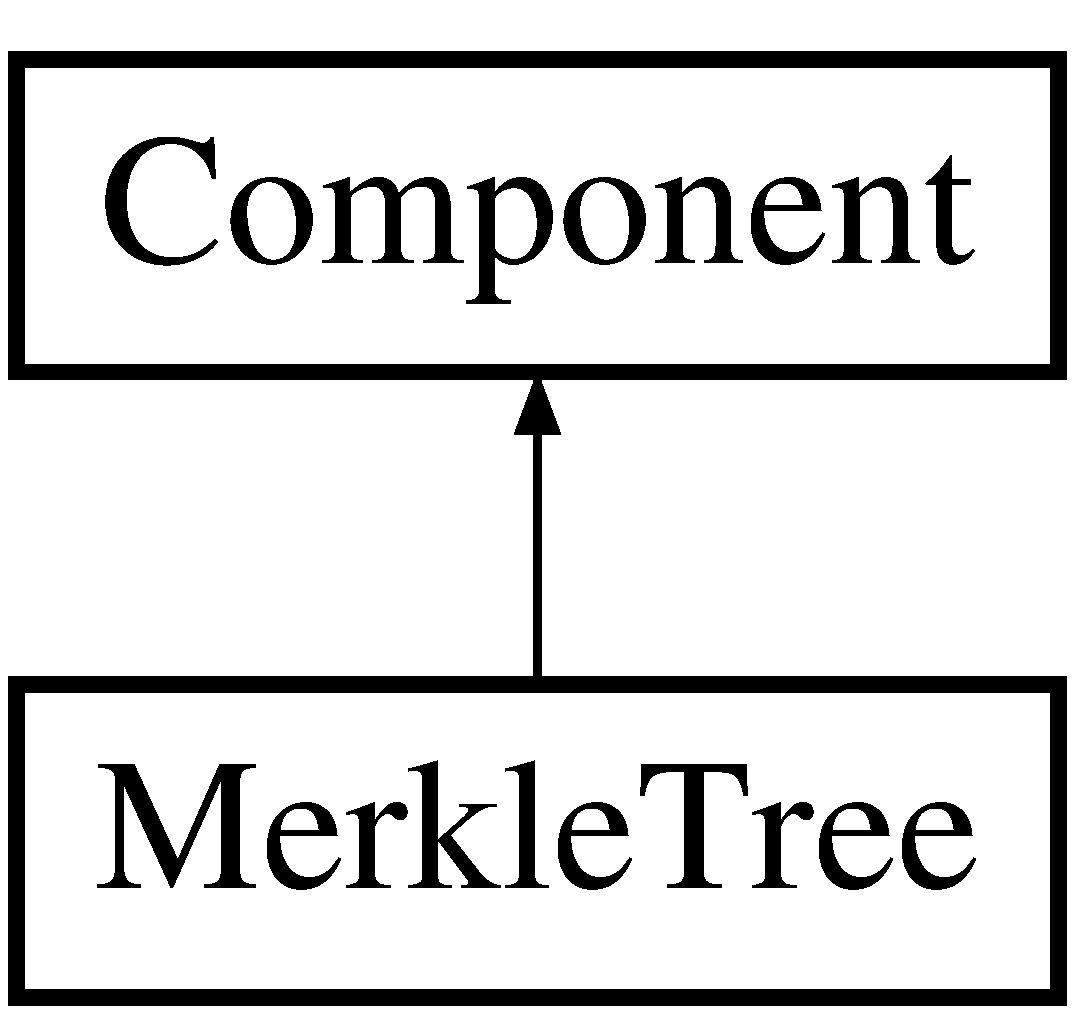
\includegraphics[height=2.000000cm]{classMerkleTree}
\end{center}
\end{figure}
\subsection*{Public Member Functions}
\begin{DoxyCompactItemize}
\item 
\mbox{\Hypertarget{classMerkleTree_a257abaf20fa542b29dfdab95294ae578}\label{classMerkleTree_a257abaf20fa542b29dfdab95294ae578}} 
{\bfseries Merkle\+Tree} (\mbox{\hyperlink{classTransaction}{Transaction}} $\ast$transaction, const \mbox{\hyperlink{classSerializer}{Serializer}} $\ast$serializer, const char $\ast$encoding)
\item 
\mbox{\Hypertarget{classMerkleTree_abc65d820b1b59f00350b2f4a4bc580bd}\label{classMerkleTree_abc65d820b1b59f00350b2f4a4bc580bd}} 
{\bfseries Merkle\+Tree} (std\+::vector$<$ \mbox{\hyperlink{classTransaction}{Transaction}} $\ast$$>$ transactions, const \mbox{\hyperlink{classSerializer}{Serializer}} $\ast$serializer, const char $\ast$encoding)
\item 
\mbox{\Hypertarget{classMerkleTree_a361a5f238249d4893b000560dcabacde}\label{classMerkleTree_a361a5f238249d4893b000560dcabacde}} 
{\bfseries Merkle\+Tree} (\mbox{\hyperlink{classMerkleTree}{Merkle\+Tree}} $\ast$l, \mbox{\hyperlink{classMerkleTree}{Merkle\+Tree}} $\ast$r)
\item 
\mbox{\hyperlink{classElement}{Element}} $\ast$ \mbox{\hyperlink{classMerkleTree_a4e72819c6cbc49ed8ce092f464711a5f}{to\+Element}} () const override
\item 
\mbox{\Hypertarget{classMerkleTree_a74d741770514ec323521ec6d79d250f2}\label{classMerkleTree_a74d741770514ec323521ec6d79d250f2}} 
\mbox{\hyperlink{classHash}{Hash}} $\ast$ {\bfseries get\+\_\+hash} (int i) const
\item 
\mbox{\Hypertarget{classMerkleTree_aac309360fa4653451af713a8ce9684bd}\label{classMerkleTree_aac309360fa4653451af713a8ce9684bd}} 
int {\bfseries size} () const
\item 
\mbox{\Hypertarget{classMerkleTree_a543fdfd1f1c4ded332cdeae2cd788aac}\label{classMerkleTree_a543fdfd1f1c4ded332cdeae2cd788aac}} 
void {\bfseries generate\+\_\+tree} (std\+::vector$<$ \mbox{\hyperlink{classTransaction}{Transaction}} $\ast$$>$ transactions, int begin, int end, const \mbox{\hyperlink{classSerializer}{Serializer}} $\ast$serializer, const char $\ast$encoding)
\item 
void \mbox{\hyperlink{classComponent_a28212595f8ee85fe009bd233bc99b2fc}{\+\_\+\+\_\+init\+\_\+\+\_\+}} (\mbox{\hyperlink{classElementObject}{Element\+Object}} $\ast$element, const \mbox{\hyperlink{classSerializer}{Serializer}} $\ast$s, const char $\ast$encoding)
\end{DoxyCompactItemize}
\subsection*{Protected Member Functions}
\begin{DoxyCompactItemize}
\item 
void \mbox{\hyperlink{classMerkleTree_a083ad348bfd770f2400f190112ff39a3}{from\+Element}} (\mbox{\hyperlink{classElementObject}{Element\+Object}} $\ast$, const \mbox{\hyperlink{classSerializer}{Serializer}} $\ast$, const char $\ast$encoding) override
\end{DoxyCompactItemize}
\subsection*{Friends}
\begin{DoxyCompactItemize}
\item 
\mbox{\Hypertarget{classMerkleTree_a6db9d28bd448a131448276ee03de1e6d}\label{classMerkleTree_a6db9d28bd448a131448276ee03de1e6d}} 
class {\bfseries Node}
\item 
\mbox{\Hypertarget{classMerkleTree_a658ef47bd757fd5e0f13adab5a417ced}\label{classMerkleTree_a658ef47bd757fd5e0f13adab5a417ced}} 
class {\bfseries Message}
\item 
\mbox{\Hypertarget{classMerkleTree_a6a4f3eb8755476d75f7f57cef4cd3853}\label{classMerkleTree_a6a4f3eb8755476d75f7f57cef4cd3853}} 
class {\bfseries Transaction\+Message}
\item 
\mbox{\Hypertarget{classMerkleTree_a760b1478b5214c122458f0f19d45c127}\label{classMerkleTree_a760b1478b5214c122458f0f19d45c127}} 
class {\bfseries Transaction\+Parser}
\item 
\mbox{\Hypertarget{classMerkleTree_a9acb1bbbd9c9589da9453187cfb6a794}\label{classMerkleTree_a9acb1bbbd9c9589da9453187cfb6a794}} 
class {\bfseries Block\+Message}
\end{DoxyCompactItemize}


\subsection{Member Function Documentation}
\mbox{\Hypertarget{classComponent_a28212595f8ee85fe009bd233bc99b2fc}\label{classComponent_a28212595f8ee85fe009bd233bc99b2fc}} 
\index{Merkle\+Tree@{Merkle\+Tree}!\+\_\+\+\_\+init\+\_\+\+\_\+@{\+\_\+\+\_\+init\+\_\+\+\_\+}}
\index{\+\_\+\+\_\+init\+\_\+\+\_\+@{\+\_\+\+\_\+init\+\_\+\+\_\+}!Merkle\+Tree@{Merkle\+Tree}}
\subsubsection{\texorpdfstring{\+\_\+\+\_\+init\+\_\+\+\_\+()}{\_\_init\_\_()}}
{\footnotesize\ttfamily void Component\+::\+\_\+\+\_\+init\+\_\+\+\_\+ (\begin{DoxyParamCaption}\item[{\mbox{\hyperlink{classElementObject}{Element\+Object}} $\ast$}]{element,  }\item[{const \mbox{\hyperlink{classSerializer}{Serializer}} $\ast$}]{s,  }\item[{const char $\ast$}]{encoding }\end{DoxyParamCaption})\hspace{0.3cm}{\ttfamily [inline]}, {\ttfamily [inherited]}}

The function called by the serializer to initialize the object if it is empty \begin{DoxySeeAlso}{See also}
\mbox{\hyperlink{classElementObject}{Element\+Object}} 

\mbox{\hyperlink{classSerializer}{Serializer}}
\end{DoxySeeAlso}

\begin{DoxyParams}{Parameters}
{\em element} & The \mbox{\hyperlink{classElement}{Element}} representation of the object \\
\hline
{\em s} & The serializer (Can be used if serialization of some elements is needed) \\
\hline
{\em encoding} & The encoding that has been used to create the \mbox{\hyperlink{classElement}{Element}} representation of the object (Can be used if serialization of some elements is needed) \\
\hline
\end{DoxyParams}
\mbox{\Hypertarget{classMerkleTree_a083ad348bfd770f2400f190112ff39a3}\label{classMerkleTree_a083ad348bfd770f2400f190112ff39a3}} 
\index{Merkle\+Tree@{Merkle\+Tree}!from\+Element@{from\+Element}}
\index{from\+Element@{from\+Element}!Merkle\+Tree@{Merkle\+Tree}}
\subsubsection{\texorpdfstring{from\+Element()}{fromElement()}}
{\footnotesize\ttfamily void Merkle\+Tree\+::from\+Element (\begin{DoxyParamCaption}\item[{\mbox{\hyperlink{classElementObject}{Element\+Object}} $\ast$}]{,  }\item[{const \mbox{\hyperlink{classSerializer}{Serializer}} $\ast$}]{,  }\item[{const char $\ast$}]{encoding }\end{DoxyParamCaption})\hspace{0.3cm}{\ttfamily [override]}, {\ttfamily [protected]}, {\ttfamily [virtual]}}

The function used to build the object from its element representation. the object if it is empty \begin{DoxySeeAlso}{See also}
\mbox{\hyperlink{classElementObject}{Element\+Object}} 

\mbox{\hyperlink{classSerializer}{Serializer}}
\end{DoxySeeAlso}

\begin{DoxyParams}{Parameters}
{\em element} & The \mbox{\hyperlink{classElement}{Element}} representation of the object \\
\hline
{\em s} & The serializer (Can be used if serialization of some elements is needed) \\
\hline
{\em encoding} & The encoding that has been used to create the \mbox{\hyperlink{classElement}{Element}} representation of the object (Can be used if serialization of some elements is needed) \\
\hline
\end{DoxyParams}


Implements \mbox{\hyperlink{classComponent_a2ded18881226d0077dc393e0e9304bb1}{Component}}.

\mbox{\Hypertarget{classMerkleTree_a4e72819c6cbc49ed8ce092f464711a5f}\label{classMerkleTree_a4e72819c6cbc49ed8ce092f464711a5f}} 
\index{Merkle\+Tree@{Merkle\+Tree}!to\+Element@{to\+Element}}
\index{to\+Element@{to\+Element}!Merkle\+Tree@{Merkle\+Tree}}
\subsubsection{\texorpdfstring{to\+Element()}{toElement()}}
{\footnotesize\ttfamily \mbox{\hyperlink{classElement}{Element}} $\ast$ Merkle\+Tree\+::to\+Element (\begin{DoxyParamCaption}{ }\end{DoxyParamCaption}) const\hspace{0.3cm}{\ttfamily [override]}, {\ttfamily [virtual]}}

The method used by the serializer to transform an object into an \mbox{\hyperlink{classElement}{Element}} representation. \begin{DoxySeeAlso}{See also}
\mbox{\hyperlink{classElement}{Element}}
\end{DoxySeeAlso}
\begin{DoxyReturn}{Returns}
The \mbox{\hyperlink{classElement}{Element}} representation of the object 
\end{DoxyReturn}


Implements \mbox{\hyperlink{classComponent_a3e63d8c993e417a4af3f56d65ebfc7ea}{Component}}.



The documentation for this class was generated from the following files\+:\begin{DoxyCompactItemize}
\item 
block\+\_\+chain/algorithm/Merkle\+Tree.\+h\item 
block\+\_\+chain/algorithm/Merkle\+Tree.\+cpp\end{DoxyCompactItemize}

\hypertarget{classMessage}{}\section{Message Class Reference}
\label{classMessage}\index{Message@{Message}}


{\ttfamily \#include $<$Message.\+h$>$}

Inheritance diagram for Message\+:\begin{figure}[H]
\begin{center}
\leavevmode
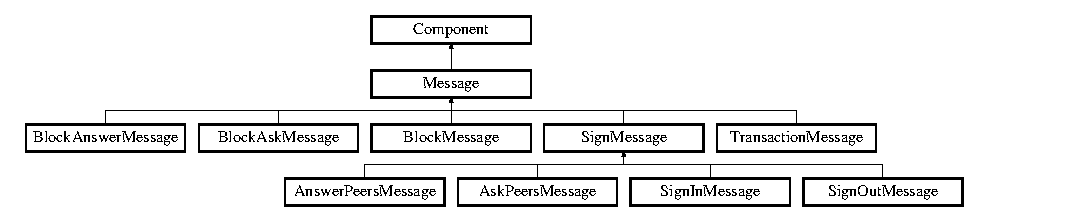
\includegraphics[height=2.539683cm]{classMessage}
\end{center}
\end{figure}
\subsection*{Public Member Functions}
\begin{DoxyCompactItemize}
\item 
\mbox{\hyperlink{classMessage_a4fc4f717b634e66070366cb7722d7761}{Message}} ()
\item 
\mbox{\hyperlink{classMessage_a6819ef42fb87c15b413b142eb96fe536}{Message}} (int i)
\item 
\mbox{\hyperlink{classMessage_aefaeef0caed942ae0920bea838065b0a}{$\sim$\+Message}} () override
\item 
const int \mbox{\hyperlink{classMessage_a2a576dcffd45c4574fcdf2897ec26086}{get\+\_\+type}} () const
\item 
virtual \mbox{\hyperlink{classElement}{Element}} $\ast$ \mbox{\hyperlink{classComponent_a3e63d8c993e417a4af3f56d65ebfc7ea}{to\+Element}} () const =0
\item 
void \mbox{\hyperlink{classComponent_a28212595f8ee85fe009bd233bc99b2fc}{\+\_\+\+\_\+init\+\_\+\+\_\+}} (\mbox{\hyperlink{classElementObject}{Element\+Object}} $\ast$element, const \mbox{\hyperlink{classSerializer}{Serializer}} $\ast$s, const char $\ast$encoding)
\end{DoxyCompactItemize}
\subsection*{Static Public Member Functions}
\begin{DoxyCompactItemize}
\item 
static \mbox{\hyperlink{classMessage}{Message}} $\ast$ \mbox{\hyperlink{classMessage_ad92a0e1cfa5b5a503ec9c61833e3e5ea}{generate}} (int id)
\end{DoxyCompactItemize}
\subsection*{Static Public Attributes}
\begin{DoxyCompactItemize}
\item 
\mbox{\Hypertarget{classMessage_a18a7a0d3879210c798f3d84c820f03c1}\label{classMessage_a18a7a0d3879210c798f3d84c820f03c1}} 
static const int {\bfseries T\+R\+A\+N\+S\+A\+C\+T\+I\+ON} = 4
\item 
\mbox{\Hypertarget{classMessage_a3d3ef3111518cd65c0b7f5ec6660888a}\label{classMessage_a3d3ef3111518cd65c0b7f5ec6660888a}} 
static const int {\bfseries B\+L\+O\+CK} = 5
\item 
\mbox{\Hypertarget{classMessage_a9810d3cefb1b33e709cb393583a7a877}\label{classMessage_a9810d3cefb1b33e709cb393583a7a877}} 
static const int {\bfseries A\+S\+K\+\_\+\+P\+E\+E\+RS} = 0
\item 
\mbox{\Hypertarget{classMessage_aa33f42e5795c4df01c7437961d512eaa}\label{classMessage_aa33f42e5795c4df01c7437961d512eaa}} 
static const int {\bfseries A\+N\+S\+W\+E\+R\+\_\+\+P\+E\+E\+RS} = 1
\item 
\mbox{\Hypertarget{classMessage_a64b7688dfdd50a6254bf45b51d2118d4}\label{classMessage_a64b7688dfdd50a6254bf45b51d2118d4}} 
static const int {\bfseries S\+I\+G\+N\+\_\+\+IN} = 2
\item 
\mbox{\Hypertarget{classMessage_aba70c352293fee66004d729ccef3ee48}\label{classMessage_aba70c352293fee66004d729ccef3ee48}} 
static const int {\bfseries S\+I\+G\+N\+\_\+\+O\+UT} = 3
\item 
\mbox{\Hypertarget{classMessage_a62ac5b91838e79a11079869015261e14}\label{classMessage_a62ac5b91838e79a11079869015261e14}} 
static const int {\bfseries A\+S\+K\+\_\+\+B\+L\+O\+CK} = 6
\item 
\mbox{\Hypertarget{classMessage_a1580f4a26d125f71e2af1ef6001ac656}\label{classMessage_a1580f4a26d125f71e2af1ef6001ac656}} 
static const int {\bfseries A\+N\+S\+W\+E\+R\+\_\+\+B\+L\+O\+CK} = 7
\end{DoxyCompactItemize}
\subsection*{Protected Member Functions}
\begin{DoxyCompactItemize}
\item 
virtual void \mbox{\hyperlink{classComponent_a2ded18881226d0077dc393e0e9304bb1}{from\+Element}} (\mbox{\hyperlink{classElementObject}{Element\+Object}} $\ast$, const \mbox{\hyperlink{classSerializer}{Serializer}} $\ast$, const char $\ast$encoding)=0
\end{DoxyCompactItemize}
\subsection*{Protected Attributes}
\begin{DoxyCompactItemize}
\item 
int \mbox{\hyperlink{classMessage_afbfb481c98b13d0deba0bac443bebe29}{type}}
\end{DoxyCompactItemize}


\subsection{Detailed Description}
An abstract message and a message factory. A message is a way to ask requests to an other peer. All different messages have different action on the current peer.

\begin{DoxyAuthor}{Author}
Mathieu Lochet 
\end{DoxyAuthor}
\begin{DoxyVersion}{Version}
2 
\end{DoxyVersion}


\subsection{Constructor \& Destructor Documentation}
\mbox{\Hypertarget{classMessage_a4fc4f717b634e66070366cb7722d7761}\label{classMessage_a4fc4f717b634e66070366cb7722d7761}} 
\index{Message@{Message}!Message@{Message}}
\index{Message@{Message}!Message@{Message}}
\subsubsection{\texorpdfstring{Message()}{Message()}\hspace{0.1cm}{\footnotesize\ttfamily [1/2]}}
{\footnotesize\ttfamily Message\+::\+Message (\begin{DoxyParamCaption}{ }\end{DoxyParamCaption})\hspace{0.3cm}{\ttfamily [default]}}

A default contructor \mbox{\Hypertarget{classMessage_a6819ef42fb87c15b413b142eb96fe536}\label{classMessage_a6819ef42fb87c15b413b142eb96fe536}} 
\index{Message@{Message}!Message@{Message}}
\index{Message@{Message}!Message@{Message}}
\subsubsection{\texorpdfstring{Message()}{Message()}\hspace{0.1cm}{\footnotesize\ttfamily [2/2]}}
{\footnotesize\ttfamily Message\+::\+Message (\begin{DoxyParamCaption}\item[{int}]{i }\end{DoxyParamCaption})\hspace{0.3cm}{\ttfamily [explicit]}}

A constructor to create a message of a given type


\begin{DoxyParams}{Parameters}
{\em i} & the given type of the message \\
\hline
\end{DoxyParams}
\mbox{\Hypertarget{classMessage_aefaeef0caed942ae0920bea838065b0a}\label{classMessage_aefaeef0caed942ae0920bea838065b0a}} 
\index{Message@{Message}!````~Message@{$\sim$\+Message}}
\index{````~Message@{$\sim$\+Message}!Message@{Message}}
\subsubsection{\texorpdfstring{$\sim$\+Message()}{~Message()}}
{\footnotesize\ttfamily Message\+::$\sim$\+Message (\begin{DoxyParamCaption}{ }\end{DoxyParamCaption})\hspace{0.3cm}{\ttfamily [override]}, {\ttfamily [default]}}

A default destructor 

\subsection{Member Function Documentation}
\mbox{\Hypertarget{classComponent_a28212595f8ee85fe009bd233bc99b2fc}\label{classComponent_a28212595f8ee85fe009bd233bc99b2fc}} 
\index{Message@{Message}!\+\_\+\+\_\+init\+\_\+\+\_\+@{\+\_\+\+\_\+init\+\_\+\+\_\+}}
\index{\+\_\+\+\_\+init\+\_\+\+\_\+@{\+\_\+\+\_\+init\+\_\+\+\_\+}!Message@{Message}}
\subsubsection{\texorpdfstring{\+\_\+\+\_\+init\+\_\+\+\_\+()}{\_\_init\_\_()}}
{\footnotesize\ttfamily void Component\+::\+\_\+\+\_\+init\+\_\+\+\_\+ (\begin{DoxyParamCaption}\item[{\mbox{\hyperlink{classElementObject}{Element\+Object}} $\ast$}]{element,  }\item[{const \mbox{\hyperlink{classSerializer}{Serializer}} $\ast$}]{s,  }\item[{const char $\ast$}]{encoding }\end{DoxyParamCaption})\hspace{0.3cm}{\ttfamily [inline]}, {\ttfamily [inherited]}}

The function called by the serializer to initialize the object if it is empty \begin{DoxySeeAlso}{See also}
\mbox{\hyperlink{classElementObject}{Element\+Object}} 

\mbox{\hyperlink{classSerializer}{Serializer}}
\end{DoxySeeAlso}

\begin{DoxyParams}{Parameters}
{\em element} & The \mbox{\hyperlink{classElement}{Element}} representation of the object \\
\hline
{\em s} & The serializer (Can be used if serialization of some elements is needed) \\
\hline
{\em encoding} & The encoding that has been used to create the \mbox{\hyperlink{classElement}{Element}} representation of the object (Can be used if serialization of some elements is needed) \\
\hline
\end{DoxyParams}
\mbox{\Hypertarget{classComponent_a2ded18881226d0077dc393e0e9304bb1}\label{classComponent_a2ded18881226d0077dc393e0e9304bb1}} 
\index{Message@{Message}!from\+Element@{from\+Element}}
\index{from\+Element@{from\+Element}!Message@{Message}}
\subsubsection{\texorpdfstring{from\+Element()}{fromElement()}}
{\footnotesize\ttfamily virtual void Component\+::from\+Element (\begin{DoxyParamCaption}\item[{\mbox{\hyperlink{classElementObject}{Element\+Object}} $\ast$}]{,  }\item[{const \mbox{\hyperlink{classSerializer}{Serializer}} $\ast$}]{,  }\item[{const char $\ast$}]{encoding }\end{DoxyParamCaption})\hspace{0.3cm}{\ttfamily [protected]}, {\ttfamily [pure virtual]}, {\ttfamily [inherited]}}

The function used to build the object from its element representation. the object if it is empty \begin{DoxySeeAlso}{See also}
\mbox{\hyperlink{classElementObject}{Element\+Object}} 

\mbox{\hyperlink{classSerializer}{Serializer}}
\end{DoxySeeAlso}

\begin{DoxyParams}{Parameters}
{\em element} & The \mbox{\hyperlink{classElement}{Element}} representation of the object \\
\hline
{\em s} & The serializer (Can be used if serialization of some elements is needed) \\
\hline
{\em encoding} & The encoding that has been used to create the \mbox{\hyperlink{classElement}{Element}} representation of the object (Can be used if serialization of some elements is needed) \\
\hline
\end{DoxyParams}


Implemented in \mbox{\hyperlink{classBlock_ab21c6536cf7a26fdf2a2e889a84fcb9d}{Block}}, \mbox{\hyperlink{classTransactionMessage_a2fbe322d67154d3bcbcc44943eeeb1ef}{Transaction\+Message}}, \mbox{\hyperlink{classBlockMessage_adda957e60057d72e1bc55d7b9c617188}{Block\+Message}}, \mbox{\hyperlink{classProofOfWorkMetadata_afac533eee3123bce72615ab90f7c9669}{Proof\+Of\+Work\+Metadata}}, \mbox{\hyperlink{classSignMessage_a35855647925ec76036ed4602743ed118}{Sign\+Message}}, \mbox{\hyperlink{classMessagesTransaction_aa70ed75ff16f6afa61d82458488069d4}{Messages\+Transaction}}, \mbox{\hyperlink{classReward_a6d16e21b60b7f11c7aaf0098a53118a2}{Reward}}, \mbox{\hyperlink{classMoneyTransaction_a6f4672dba3a75e2782d15366d9ed7a1e}{Money\+Transaction}}, \mbox{\hyperlink{classBlockAskMessage_a25875b2446d7ecc5f644c568c8f12df3}{Block\+Ask\+Message}}, \mbox{\hyperlink{classBlockAnswerMessage_affa76e8a95365baf5c9eb409a0a19b9d}{Block\+Answer\+Message}}, \mbox{\hyperlink{classStatusTransaction_aa05e4be5f990e8a9533383b3b7dc1382}{Status\+Transaction}}, and \mbox{\hyperlink{classMerkleTree_a083ad348bfd770f2400f190112ff39a3}{Merkle\+Tree}}.

\mbox{\Hypertarget{classMessage_ad92a0e1cfa5b5a503ec9c61833e3e5ea}\label{classMessage_ad92a0e1cfa5b5a503ec9c61833e3e5ea}} 
\index{Message@{Message}!generate@{generate}}
\index{generate@{generate}!Message@{Message}}
\subsubsection{\texorpdfstring{generate()}{generate()}}
{\footnotesize\ttfamily \mbox{\hyperlink{classMessage}{Message}} $\ast$ Message\+::generate (\begin{DoxyParamCaption}\item[{int}]{id }\end{DoxyParamCaption})\hspace{0.3cm}{\ttfamily [static]}}

The message factory\+: creates the corresponding type of message with a given type. The generated message is empty and needs to be fill. \begin{DoxySeeAlso}{See also}
\mbox{\hyperlink{classComponent}{Component}}\+:\+:{\bfseries init}
\end{DoxySeeAlso}

\begin{DoxyParams}{Parameters}
{\em id} & the given type of the wanted message \\
\hline
\end{DoxyParams}
\begin{DoxyReturn}{Returns}
The type of the message 
\end{DoxyReturn}
\mbox{\Hypertarget{classMessage_a2a576dcffd45c4574fcdf2897ec26086}\label{classMessage_a2a576dcffd45c4574fcdf2897ec26086}} 
\index{Message@{Message}!get\+\_\+type@{get\+\_\+type}}
\index{get\+\_\+type@{get\+\_\+type}!Message@{Message}}
\subsubsection{\texorpdfstring{get\+\_\+type()}{get\_type()}}
{\footnotesize\ttfamily const int Message\+::get\+\_\+type (\begin{DoxyParamCaption}{ }\end{DoxyParamCaption}) const}

Get the type of the message

\begin{DoxyReturn}{Returns}
The type of the message 
\end{DoxyReturn}
\mbox{\Hypertarget{classComponent_a3e63d8c993e417a4af3f56d65ebfc7ea}\label{classComponent_a3e63d8c993e417a4af3f56d65ebfc7ea}} 
\index{Message@{Message}!to\+Element@{to\+Element}}
\index{to\+Element@{to\+Element}!Message@{Message}}
\subsubsection{\texorpdfstring{to\+Element()}{toElement()}}
{\footnotesize\ttfamily virtual \mbox{\hyperlink{classElement}{Element}}$\ast$ Component\+::to\+Element (\begin{DoxyParamCaption}{ }\end{DoxyParamCaption}) const\hspace{0.3cm}{\ttfamily [pure virtual]}, {\ttfamily [inherited]}}

The method used by the serializer to transform an object into an \mbox{\hyperlink{classElement}{Element}} representation. \begin{DoxySeeAlso}{See also}
\mbox{\hyperlink{classElement}{Element}}
\end{DoxySeeAlso}
\begin{DoxyReturn}{Returns}
The \mbox{\hyperlink{classElement}{Element}} representation of the object 
\end{DoxyReturn}


Implemented in \mbox{\hyperlink{classBlock_aa289363a40f0d3ba88720ad0bc71f34f}{Block}}, \mbox{\hyperlink{classTransactionMessage_ae20e7d6a7b5811bb56a32ec6af59b8e2}{Transaction\+Message}}, \mbox{\hyperlink{classBlockMessage_ab47afd5cfb7d6d5c544d8def5d0f9737}{Block\+Message}}, \mbox{\hyperlink{classSignMessage_aee897c4bf78df966b8cca95e589566e4}{Sign\+Message}}, \mbox{\hyperlink{classProofOfWorkMetadata_a2aab4c26afb3a85a712cc065028274d9}{Proof\+Of\+Work\+Metadata}}, \mbox{\hyperlink{classBlockAskMessage_a0bc20076f19423855ab5772003fb65f6}{Block\+Ask\+Message}}, \mbox{\hyperlink{classBlockAnswerMessage_ac7f35ec9f7f2fbcd726628c2a984518b}{Block\+Answer\+Message}}, \mbox{\hyperlink{classReward_a0ecd536148463880f9980fe415b6eb1d}{Reward}}, \mbox{\hyperlink{classMerkleTree_a4e72819c6cbc49ed8ce092f464711a5f}{Merkle\+Tree}}, \mbox{\hyperlink{classMessagesTransaction_a0ef8ec080a2698a02ad8b1b95d243720}{Messages\+Transaction}}, \mbox{\hyperlink{classStatusTransaction_aed42f2d61f2d50ec07bb6b35473f61f2}{Status\+Transaction}}, and \mbox{\hyperlink{classMoneyTransaction_a84adc847266467965014cb04acd48bea}{Money\+Transaction}}.



\subsection{Member Data Documentation}
\mbox{\Hypertarget{classMessage_afbfb481c98b13d0deba0bac443bebe29}\label{classMessage_afbfb481c98b13d0deba0bac443bebe29}} 
\index{Message@{Message}!type@{type}}
\index{type@{type}!Message@{Message}}
\subsubsection{\texorpdfstring{type}{type}}
{\footnotesize\ttfamily int Message\+::type\hspace{0.3cm}{\ttfamily [protected]}}

The type of the message 

The documentation for this class was generated from the following files\+:\begin{DoxyCompactItemize}
\item 
block\+\_\+chain/kernel/messages/Message.\+h\item 
block\+\_\+chain/kernel/messages/Message.\+cpp\end{DoxyCompactItemize}

\hypertarget{classMessageParser}{}\section{Message\+Parser Class Reference}
\label{classMessageParser}\index{Message\+Parser@{Message\+Parser}}
Inheritance diagram for Message\+Parser\+:\begin{figure}[H]
\begin{center}
\leavevmode
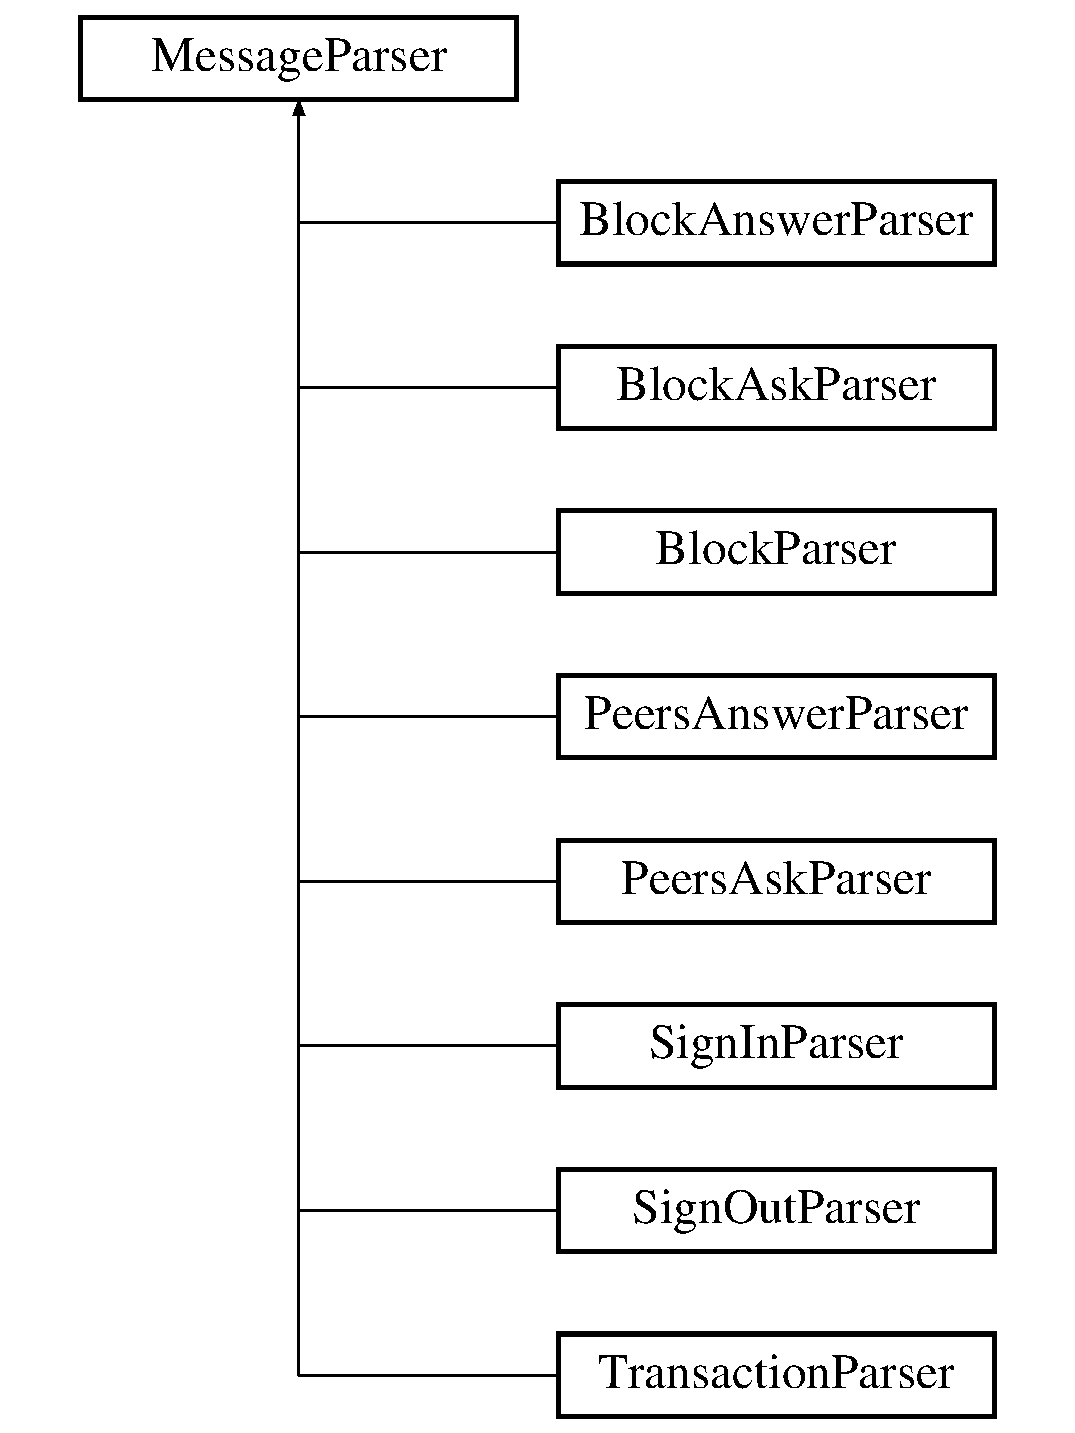
\includegraphics[height=9.000000cm]{classMessageParser}
\end{center}
\end{figure}
\subsection*{Public Member Functions}
\begin{DoxyCompactItemize}
\item 
\mbox{\Hypertarget{classMessageParser_a946f3b936dc01a75d6165329b159ecfe}\label{classMessageParser_a946f3b936dc01a75d6165329b159ecfe}} 
virtual void {\bfseries operator()} (\mbox{\hyperlink{classMessage}{Message}} $\ast$m, \mbox{\hyperlink{classNode}{Node}} $\ast$node) const =0
\item 
\mbox{\Hypertarget{classMessageParser_aa7c495d7b28a394e5752ca25ffff69d8}\label{classMessageParser_aa7c495d7b28a394e5752ca25ffff69d8}} 
virtual int {\bfseries get\+\_\+type} () const =0
\end{DoxyCompactItemize}


The documentation for this class was generated from the following file\+:\begin{DoxyCompactItemize}
\item 
block\+\_\+chain/kernel/parsers/Message\+Parser.\+h\end{DoxyCompactItemize}

\hypertarget{classMessagesTransaction}{}\section{Messages\+Transaction Class Reference}
\label{classMessagesTransaction}\index{Messages\+Transaction@{Messages\+Transaction}}
Inheritance diagram for Messages\+Transaction\+:\begin{figure}[H]
\begin{center}
\leavevmode
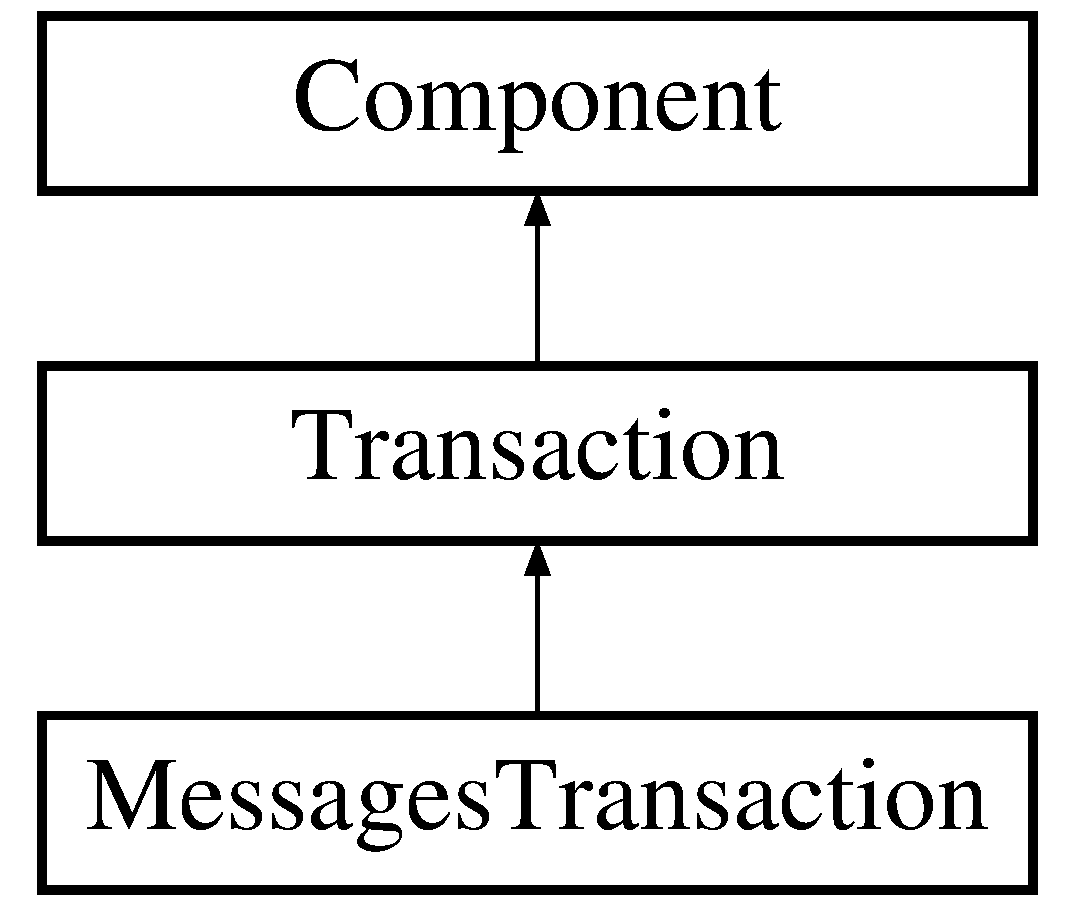
\includegraphics[height=3.000000cm]{classMessagesTransaction}
\end{center}
\end{figure}
\subsection*{Public Member Functions}
\begin{DoxyCompactItemize}
\item 
\mbox{\Hypertarget{classMessagesTransaction_ad11ea6fc9104b441c520bde2ae542309}\label{classMessagesTransaction_ad11ea6fc9104b441c520bde2ae542309}} 
bool {\bfseries operator()} () const final
\item 
\mbox{\Hypertarget{classMessagesTransaction_a0ef8ec080a2698a02ad8b1b95d243720}\label{classMessagesTransaction_a0ef8ec080a2698a02ad8b1b95d243720}} 
\mbox{\hyperlink{classElement}{Element}} $\ast$ {\bfseries to\+Element} () const override
\item 
\mbox{\Hypertarget{classMessagesTransaction_aeeffbaa69d8432b6c12ca8fdf66e2e8b}\label{classMessagesTransaction_aeeffbaa69d8432b6c12ca8fdf66e2e8b}} 
bool {\bfseries operator==} (\mbox{\hyperlink{classTransaction}{Transaction}} $\ast$t) const override
\item 
\mbox{\Hypertarget{classMessagesTransaction_ac29f29d1f9d168eb82411438805a11ee}\label{classMessagesTransaction_ac29f29d1f9d168eb82411438805a11ee}} 
std\+::string {\bfseries to\+\_\+string} () const
\item 
\mbox{\Hypertarget{classMessagesTransaction_af39b2220f345169fa3276597f38681d5}\label{classMessagesTransaction_af39b2220f345169fa3276597f38681d5}} 
std\+::vector$<$ std\+::string $>$ {\bfseries apply} (\mbox{\hyperlink{classRow}{Row}} $\ast$row) override
\item 
\mbox{\Hypertarget{classMessagesTransaction_a3eec18f09aa102b3cee7f215c225a8fb}\label{classMessagesTransaction_a3eec18f09aa102b3cee7f215c225a8fb}} 
\mbox{\hyperlink{classRow}{Row}} $\ast$ {\bfseries create\+Row} () const override
\item 
\mbox{\Hypertarget{classMessagesTransaction_ad44d1a3d26383c153360d3836606b7ce}\label{classMessagesTransaction_ad44d1a3d26383c153360d3836606b7ce}} 
void {\bfseries apply\+\_\+reverse} (\mbox{\hyperlink{classRow}{Row}} $\ast$row) override
\item 
\mbox{\Hypertarget{classMessagesTransaction_a59a0d03ac175701616ce341947f9cd64}\label{classMessagesTransaction_a59a0d03ac175701616ce341947f9cd64}} 
bool {\bfseries validate} (\mbox{\hyperlink{classRow}{Row}} $\ast$row) const override
\item 
\mbox{\Hypertarget{classMessagesTransaction_a1893ac38468108811eb396366a3c0454}\label{classMessagesTransaction_a1893ac38468108811eb396366a3c0454}} 
int {\bfseries get\+\_\+type} () const override
\item 
\mbox{\Hypertarget{classMessagesTransaction_a8cf65215291254275a1dd989f0971bd4}\label{classMessagesTransaction_a8cf65215291254275a1dd989f0971bd4}} 
std\+::string {\bfseries description} () const override
\item 
\mbox{\Hypertarget{classMessagesTransaction_aeca5802e7f1bd57e38468dc3394e2825}\label{classMessagesTransaction_aeca5802e7f1bd57e38468dc3394e2825}} 
void {\bfseries fill\+\_\+data} () override
\item 
\mbox{\Hypertarget{classMessagesTransaction_a290e38ea445bba3f62956c660607c03f}\label{classMessagesTransaction_a290e38ea445bba3f62956c660607c03f}} 
\mbox{\hyperlink{classTransaction}{Transaction}} $\ast$ {\bfseries clone} () override
\item 
\mbox{\Hypertarget{classTransaction_a1f0df166c34d6a38a991544cf98c0356}\label{classTransaction_a1f0df166c34d6a38a991544cf98c0356}} 
\mbox{\hyperlink{classHash}{Hash}} $\ast$ {\bfseries \+\_\+\+\_\+hash\+\_\+\+\_\+} (const \mbox{\hyperlink{classSerializer}{Serializer}} $\ast$serializer, const char $\ast$encoding) const
\item 
\mbox{\Hypertarget{classComponent_a28212595f8ee85fe009bd233bc99b2fc}\label{classComponent_a28212595f8ee85fe009bd233bc99b2fc}} 
void {\bfseries \+\_\+\+\_\+init\+\_\+\+\_\+} (\mbox{\hyperlink{classElementObject}{Element\+Object}} $\ast$element, const \mbox{\hyperlink{classSerializer}{Serializer}} $\ast$s, const char $\ast$encoding)
\end{DoxyCompactItemize}
\subsection*{Protected Member Functions}
\begin{DoxyCompactItemize}
\item 
\mbox{\Hypertarget{classMessagesTransaction_aa70ed75ff16f6afa61d82458488069d4}\label{classMessagesTransaction_aa70ed75ff16f6afa61d82458488069d4}} 
void {\bfseries from\+Element} (\mbox{\hyperlink{classElementObject}{Element\+Object}} $\ast$, const \mbox{\hyperlink{classSerializer}{Serializer}} $\ast$, const char $\ast$encoding) override
\end{DoxyCompactItemize}


The documentation for this class was generated from the following files\+:\begin{DoxyCompactItemize}
\item 
transactions/Messages\+Transaction.\+h\item 
transactions/Messages\+Transaction.\+cpp\end{DoxyCompactItemize}

\hypertarget{classMetadata}{}\section{Metadata Class Reference}
\label{classMetadata}\index{Metadata@{Metadata}}


{\ttfamily \#include $<$Metadata.\+h$>$}

Inheritance diagram for Metadata\+:\begin{figure}[H]
\begin{center}
\leavevmode
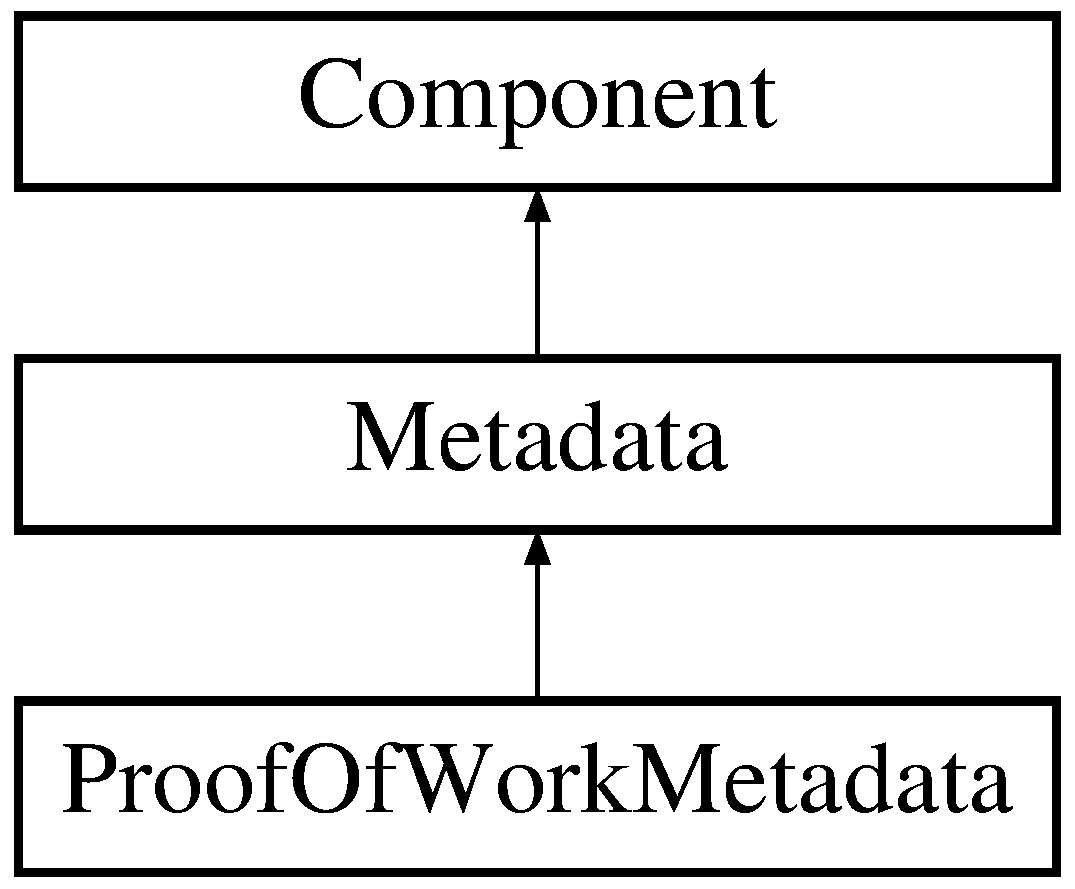
\includegraphics[height=3.000000cm]{classMetadata}
\end{center}
\end{figure}
\subsection*{Public Member Functions}
\begin{DoxyCompactItemize}
\item 
virtual \mbox{\hyperlink{classMetadata_a29845232ba882e6dba16311f2ae4c374}{$\sim$\+Metadata}} ()
\item 
virtual bool \mbox{\hyperlink{classMetadata_a2721356452a5d366d58275dd1fc1209c}{operator==}} (\mbox{\hyperlink{classMetadata}{Metadata}} \&m) const
\item 
virtual void \mbox{\hyperlink{classMetadata_a501ab1977aac6a75f92309284e17de30}{update\+\_\+database}} (\mbox{\hyperlink{classDatabase}{Database}} $\ast$d)=0
\item 
virtual \mbox{\hyperlink{classHash}{Hash}} $\ast$ \mbox{\hyperlink{classMetadata_a893b85a8fe38060c72bdda20818a7334}{hash}} ()=0
\item 
virtual \mbox{\hyperlink{classElement}{Element}} $\ast$ \mbox{\hyperlink{classComponent_a3e63d8c993e417a4af3f56d65ebfc7ea}{to\+Element}} () const =0
\item 
void \mbox{\hyperlink{classComponent_a28212595f8ee85fe009bd233bc99b2fc}{\+\_\+\+\_\+init\+\_\+\+\_\+}} (\mbox{\hyperlink{classElementObject}{Element\+Object}} $\ast$element, const \mbox{\hyperlink{classSerializer}{Serializer}} $\ast$s, const char $\ast$encoding)
\end{DoxyCompactItemize}
\subsection*{Protected Member Functions}
\begin{DoxyCompactItemize}
\item 
virtual void \mbox{\hyperlink{classComponent_a2ded18881226d0077dc393e0e9304bb1}{from\+Element}} (\mbox{\hyperlink{classElementObject}{Element\+Object}} $\ast$, const \mbox{\hyperlink{classSerializer}{Serializer}} $\ast$, const char $\ast$encoding)=0
\end{DoxyCompactItemize}


\subsection{Detailed Description}
An abstract metadata class representing a block\textquotesingle{}s header. Needs to be reimplemented with the proper header representation \begin{DoxySeeAlso}{See also}
\mbox{\hyperlink{classBlock}{Block}}
\end{DoxySeeAlso}
\begin{DoxyAuthor}{Author}
Mathieu Lochet 
\end{DoxyAuthor}
\begin{DoxyVersion}{Version}
2 
\end{DoxyVersion}


\subsection{Constructor \& Destructor Documentation}
\mbox{\Hypertarget{classMetadata_a29845232ba882e6dba16311f2ae4c374}\label{classMetadata_a29845232ba882e6dba16311f2ae4c374}} 
\index{Metadata@{Metadata}!````~Metadata@{$\sim$\+Metadata}}
\index{````~Metadata@{$\sim$\+Metadata}!Metadata@{Metadata}}
\subsubsection{\texorpdfstring{$\sim$\+Metadata()}{~Metadata()}}
{\footnotesize\ttfamily Metadata\+::$\sim$\+Metadata (\begin{DoxyParamCaption}{ }\end{DoxyParamCaption})\hspace{0.3cm}{\ttfamily [virtual]}}

A virtual default destructor 

\subsection{Member Function Documentation}
\mbox{\Hypertarget{classComponent_a28212595f8ee85fe009bd233bc99b2fc}\label{classComponent_a28212595f8ee85fe009bd233bc99b2fc}} 
\index{Metadata@{Metadata}!\+\_\+\+\_\+init\+\_\+\+\_\+@{\+\_\+\+\_\+init\+\_\+\+\_\+}}
\index{\+\_\+\+\_\+init\+\_\+\+\_\+@{\+\_\+\+\_\+init\+\_\+\+\_\+}!Metadata@{Metadata}}
\subsubsection{\texorpdfstring{\+\_\+\+\_\+init\+\_\+\+\_\+()}{\_\_init\_\_()}}
{\footnotesize\ttfamily void Component\+::\+\_\+\+\_\+init\+\_\+\+\_\+ (\begin{DoxyParamCaption}\item[{\mbox{\hyperlink{classElementObject}{Element\+Object}} $\ast$}]{element,  }\item[{const \mbox{\hyperlink{classSerializer}{Serializer}} $\ast$}]{s,  }\item[{const char $\ast$}]{encoding }\end{DoxyParamCaption})\hspace{0.3cm}{\ttfamily [inline]}, {\ttfamily [inherited]}}

The function called by the serializer to initialize the object if it is empty \begin{DoxySeeAlso}{See also}
\mbox{\hyperlink{classElementObject}{Element\+Object}} 

\mbox{\hyperlink{classSerializer}{Serializer}}
\end{DoxySeeAlso}

\begin{DoxyParams}{Parameters}
{\em element} & The \mbox{\hyperlink{classElement}{Element}} representation of the object \\
\hline
{\em s} & The serializer (Can be used if serialization of some elements is needed) \\
\hline
{\em encoding} & The encoding that has been used to create the \mbox{\hyperlink{classElement}{Element}} representation of the object (Can be used if serialization of some elements is needed) \\
\hline
\end{DoxyParams}
\mbox{\Hypertarget{classComponent_a2ded18881226d0077dc393e0e9304bb1}\label{classComponent_a2ded18881226d0077dc393e0e9304bb1}} 
\index{Metadata@{Metadata}!from\+Element@{from\+Element}}
\index{from\+Element@{from\+Element}!Metadata@{Metadata}}
\subsubsection{\texorpdfstring{from\+Element()}{fromElement()}}
{\footnotesize\ttfamily virtual void Component\+::from\+Element (\begin{DoxyParamCaption}\item[{\mbox{\hyperlink{classElementObject}{Element\+Object}} $\ast$}]{,  }\item[{const \mbox{\hyperlink{classSerializer}{Serializer}} $\ast$}]{,  }\item[{const char $\ast$}]{encoding }\end{DoxyParamCaption})\hspace{0.3cm}{\ttfamily [protected]}, {\ttfamily [pure virtual]}, {\ttfamily [inherited]}}

The function used to build the object from its element representation. the object if it is empty \begin{DoxySeeAlso}{See also}
\mbox{\hyperlink{classElementObject}{Element\+Object}} 

\mbox{\hyperlink{classSerializer}{Serializer}}
\end{DoxySeeAlso}

\begin{DoxyParams}{Parameters}
{\em element} & The \mbox{\hyperlink{classElement}{Element}} representation of the object \\
\hline
{\em s} & The serializer (Can be used if serialization of some elements is needed) \\
\hline
{\em encoding} & The encoding that has been used to create the \mbox{\hyperlink{classElement}{Element}} representation of the object (Can be used if serialization of some elements is needed) \\
\hline
\end{DoxyParams}


Implemented in \mbox{\hyperlink{classBlock_ab21c6536cf7a26fdf2a2e889a84fcb9d}{Block}}, \mbox{\hyperlink{classTransactionMessage_a2fbe322d67154d3bcbcc44943eeeb1ef}{Transaction\+Message}}, \mbox{\hyperlink{classBlockMessage_adda957e60057d72e1bc55d7b9c617188}{Block\+Message}}, \mbox{\hyperlink{classProofOfWorkMetadata_afac533eee3123bce72615ab90f7c9669}{Proof\+Of\+Work\+Metadata}}, \mbox{\hyperlink{classSignMessage_a35855647925ec76036ed4602743ed118}{Sign\+Message}}, \mbox{\hyperlink{classMessagesTransaction_aa70ed75ff16f6afa61d82458488069d4}{Messages\+Transaction}}, \mbox{\hyperlink{classReward_a6d16e21b60b7f11c7aaf0098a53118a2}{Reward}}, \mbox{\hyperlink{classMoneyTransaction_a6f4672dba3a75e2782d15366d9ed7a1e}{Money\+Transaction}}, \mbox{\hyperlink{classBlockAskMessage_a25875b2446d7ecc5f644c568c8f12df3}{Block\+Ask\+Message}}, \mbox{\hyperlink{classBlockAnswerMessage_affa76e8a95365baf5c9eb409a0a19b9d}{Block\+Answer\+Message}}, \mbox{\hyperlink{classStatusTransaction_aa05e4be5f990e8a9533383b3b7dc1382}{Status\+Transaction}}, and \mbox{\hyperlink{classMerkleTree_a083ad348bfd770f2400f190112ff39a3}{Merkle\+Tree}}.

\mbox{\Hypertarget{classMetadata_a893b85a8fe38060c72bdda20818a7334}\label{classMetadata_a893b85a8fe38060c72bdda20818a7334}} 
\index{Metadata@{Metadata}!hash@{hash}}
\index{hash@{hash}!Metadata@{Metadata}}
\subsubsection{\texorpdfstring{hash()}{hash()}}
{\footnotesize\ttfamily virtual \mbox{\hyperlink{classHash}{Hash}}$\ast$ Metadata\+::hash (\begin{DoxyParamCaption}{ }\end{DoxyParamCaption})\hspace{0.3cm}{\ttfamily [pure virtual]}}

Get the hash ofthe user who validated the block

\begin{DoxyReturn}{Returns}
The hash ofthe user who validated the block 
\end{DoxyReturn}


Implemented in \mbox{\hyperlink{classProofOfWorkMetadata_af29f8f40d4b438eaa9434b51c1aff7c6}{Proof\+Of\+Work\+Metadata}}.

\mbox{\Hypertarget{classMetadata_a2721356452a5d366d58275dd1fc1209c}\label{classMetadata_a2721356452a5d366d58275dd1fc1209c}} 
\index{Metadata@{Metadata}!operator==@{operator==}}
\index{operator==@{operator==}!Metadata@{Metadata}}
\subsubsection{\texorpdfstring{operator==()}{operator==()}}
{\footnotesize\ttfamily virtual bool Metadata\+::operator== (\begin{DoxyParamCaption}\item[{\mbox{\hyperlink{classMetadata}{Metadata}} \&}]{m }\end{DoxyParamCaption}) const\hspace{0.3cm}{\ttfamily [inline]}, {\ttfamily [virtual]}}

Overriding the == operator


\begin{DoxyParams}{Parameters}
{\em m} & A metadata to be compared \\
\hline
\end{DoxyParams}
\begin{DoxyReturn}{Returns}
true if the conditions are satisfied, false otherwise 
\end{DoxyReturn}


Reimplemented in \mbox{\hyperlink{classProofOfWorkMetadata_ae490506a28967c7180163fc156dd5d51}{Proof\+Of\+Work\+Metadata}}.

\mbox{\Hypertarget{classComponent_a3e63d8c993e417a4af3f56d65ebfc7ea}\label{classComponent_a3e63d8c993e417a4af3f56d65ebfc7ea}} 
\index{Metadata@{Metadata}!to\+Element@{to\+Element}}
\index{to\+Element@{to\+Element}!Metadata@{Metadata}}
\subsubsection{\texorpdfstring{to\+Element()}{toElement()}}
{\footnotesize\ttfamily virtual \mbox{\hyperlink{classElement}{Element}}$\ast$ Component\+::to\+Element (\begin{DoxyParamCaption}{ }\end{DoxyParamCaption}) const\hspace{0.3cm}{\ttfamily [pure virtual]}, {\ttfamily [inherited]}}

The method used by the serializer to transform an object into an \mbox{\hyperlink{classElement}{Element}} representation. \begin{DoxySeeAlso}{See also}
\mbox{\hyperlink{classElement}{Element}}
\end{DoxySeeAlso}
\begin{DoxyReturn}{Returns}
The \mbox{\hyperlink{classElement}{Element}} representation of the object 
\end{DoxyReturn}


Implemented in \mbox{\hyperlink{classBlock_aa289363a40f0d3ba88720ad0bc71f34f}{Block}}, \mbox{\hyperlink{classTransactionMessage_ae20e7d6a7b5811bb56a32ec6af59b8e2}{Transaction\+Message}}, \mbox{\hyperlink{classBlockMessage_ab47afd5cfb7d6d5c544d8def5d0f9737}{Block\+Message}}, \mbox{\hyperlink{classSignMessage_aee897c4bf78df966b8cca95e589566e4}{Sign\+Message}}, \mbox{\hyperlink{classProofOfWorkMetadata_a2aab4c26afb3a85a712cc065028274d9}{Proof\+Of\+Work\+Metadata}}, \mbox{\hyperlink{classBlockAskMessage_a0bc20076f19423855ab5772003fb65f6}{Block\+Ask\+Message}}, \mbox{\hyperlink{classBlockAnswerMessage_ac7f35ec9f7f2fbcd726628c2a984518b}{Block\+Answer\+Message}}, \mbox{\hyperlink{classReward_a0ecd536148463880f9980fe415b6eb1d}{Reward}}, \mbox{\hyperlink{classMerkleTree_a4e72819c6cbc49ed8ce092f464711a5f}{Merkle\+Tree}}, \mbox{\hyperlink{classMessagesTransaction_a0ef8ec080a2698a02ad8b1b95d243720}{Messages\+Transaction}}, \mbox{\hyperlink{classStatusTransaction_aed42f2d61f2d50ec07bb6b35473f61f2}{Status\+Transaction}}, and \mbox{\hyperlink{classMoneyTransaction_a84adc847266467965014cb04acd48bea}{Money\+Transaction}}.

\mbox{\Hypertarget{classMetadata_a501ab1977aac6a75f92309284e17de30}\label{classMetadata_a501ab1977aac6a75f92309284e17de30}} 
\index{Metadata@{Metadata}!update\+\_\+database@{update\+\_\+database}}
\index{update\+\_\+database@{update\+\_\+database}!Metadata@{Metadata}}
\subsubsection{\texorpdfstring{update\+\_\+database()}{update\_database()}}
{\footnotesize\ttfamily virtual void Metadata\+::update\+\_\+database (\begin{DoxyParamCaption}\item[{\mbox{\hyperlink{classDatabase}{Database}} $\ast$}]{d }\end{DoxyParamCaption})\hspace{0.3cm}{\ttfamily [pure virtual]}}

Update the database with the reward transaction when the block is validated


\begin{DoxyParams}{Parameters}
{\em d} & The database to update \\
\hline
\end{DoxyParams}


Implemented in \mbox{\hyperlink{classProofOfWorkMetadata_add9667954ffeaee75f3329c6c832e8b7}{Proof\+Of\+Work\+Metadata}}.



The documentation for this class was generated from the following files\+:\begin{DoxyCompactItemize}
\item 
block\+\_\+chain/chain/block/proof/metadatas/Metadata.\+h\item 
block\+\_\+chain/chain/block/proof/metadatas/Metadata.\+cpp\end{DoxyCompactItemize}

\hypertarget{classMoneyTransaction}{}\section{Money\+Transaction Class Reference}
\label{classMoneyTransaction}\index{Money\+Transaction@{Money\+Transaction}}
Inheritance diagram for Money\+Transaction\+:\begin{figure}[H]
\begin{center}
\leavevmode
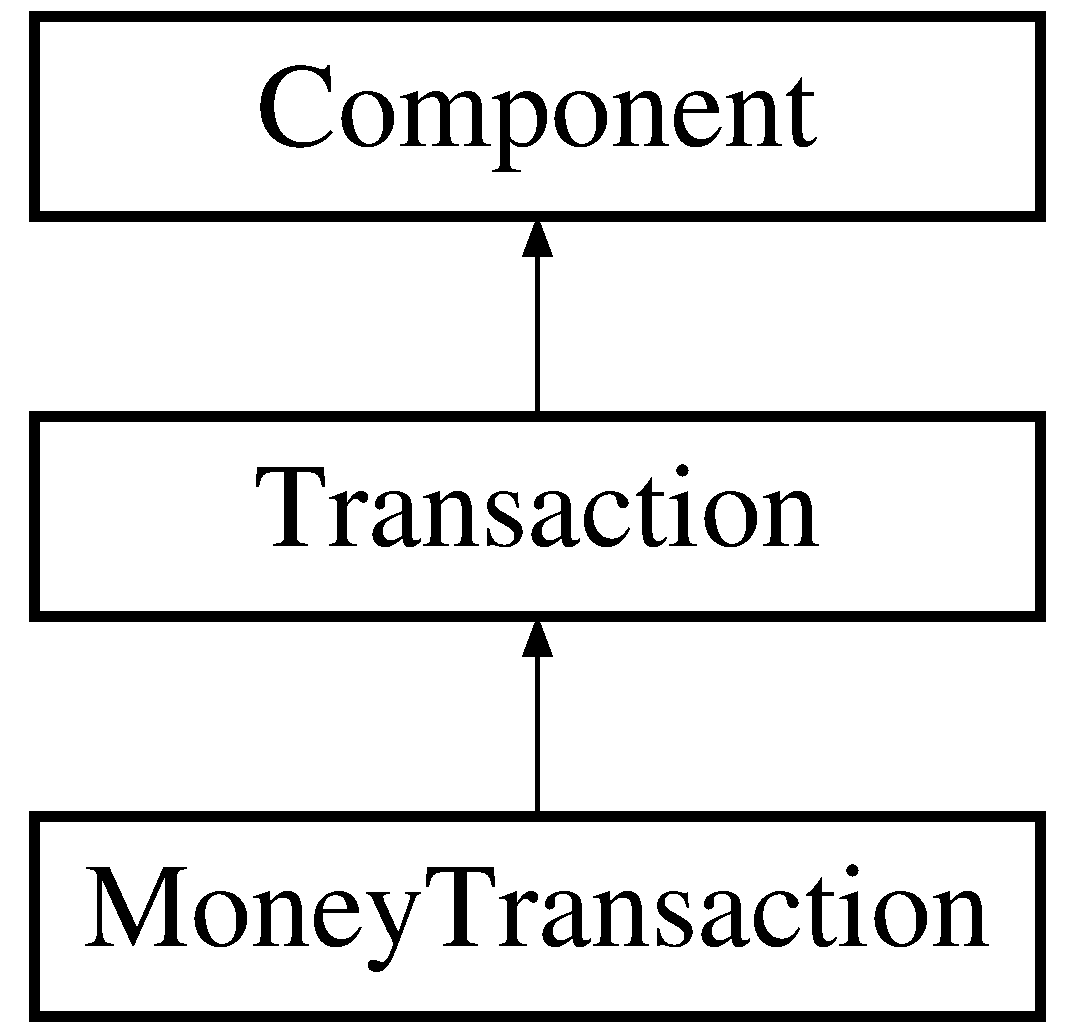
\includegraphics[height=3.000000cm]{classMoneyTransaction}
\end{center}
\end{figure}
\subsection*{Public Member Functions}
\begin{DoxyCompactItemize}
\item 
\mbox{\Hypertarget{classMoneyTransaction_aeb2a694e47dfe8ec64084af9425f8833}\label{classMoneyTransaction_aeb2a694e47dfe8ec64084af9425f8833}} 
bool {\bfseries operator()} () const final
\item 
\mbox{\Hypertarget{classMoneyTransaction_a84adc847266467965014cb04acd48bea}\label{classMoneyTransaction_a84adc847266467965014cb04acd48bea}} 
\mbox{\hyperlink{classElement}{Element}} $\ast$ {\bfseries to\+Element} () const override
\item 
\mbox{\Hypertarget{classMoneyTransaction_a9cd0b36a92155e91a25eb1b1435516d3}\label{classMoneyTransaction_a9cd0b36a92155e91a25eb1b1435516d3}} 
bool {\bfseries operator==} (\mbox{\hyperlink{classTransaction}{Transaction}} $\ast$t) const override
\item 
\mbox{\Hypertarget{classMoneyTransaction_a3ca87ee0b7fc6b84615b691ddcaf9f3c}\label{classMoneyTransaction_a3ca87ee0b7fc6b84615b691ddcaf9f3c}} 
std\+::string {\bfseries to\+\_\+string} () const
\item 
\mbox{\Hypertarget{classMoneyTransaction_a8aa6f693c524d8e1e052b616546f9647}\label{classMoneyTransaction_a8aa6f693c524d8e1e052b616546f9647}} 
std\+::vector$<$ std\+::string $>$ {\bfseries apply} (\mbox{\hyperlink{classRow}{Row}} $\ast$row) override
\item 
\mbox{\Hypertarget{classMoneyTransaction_a53b636ba053baae7705976efce629d21}\label{classMoneyTransaction_a53b636ba053baae7705976efce629d21}} 
\mbox{\hyperlink{classRow}{Row}} $\ast$ {\bfseries create\+Row} () const override
\item 
\mbox{\Hypertarget{classMoneyTransaction_a9eaa71eed1cc8b06ef5773c76c814ad9}\label{classMoneyTransaction_a9eaa71eed1cc8b06ef5773c76c814ad9}} 
void {\bfseries apply\+\_\+reverse} (\mbox{\hyperlink{classRow}{Row}} $\ast$row) override
\item 
\mbox{\Hypertarget{classMoneyTransaction_a20c58901a2aa8c51b73d56000545e82c}\label{classMoneyTransaction_a20c58901a2aa8c51b73d56000545e82c}} 
bool {\bfseries validate} (\mbox{\hyperlink{classRow}{Row}} $\ast$row) const override
\item 
\mbox{\Hypertarget{classMoneyTransaction_a705918a47c0471ee7cf82bcdf0aeb5ef}\label{classMoneyTransaction_a705918a47c0471ee7cf82bcdf0aeb5ef}} 
int {\bfseries get\+\_\+type} () const override
\item 
\mbox{\Hypertarget{classMoneyTransaction_a23b793077f5c5e3157155df148e0d5e1}\label{classMoneyTransaction_a23b793077f5c5e3157155df148e0d5e1}} 
std\+::string {\bfseries description} () const override
\item 
\mbox{\Hypertarget{classMoneyTransaction_a8666737a342f5eb1856006cd970967bf}\label{classMoneyTransaction_a8666737a342f5eb1856006cd970967bf}} 
void {\bfseries fill\+\_\+data} () override
\item 
\mbox{\Hypertarget{classMoneyTransaction_af777b46f577df3c089a44c78c1aebc40}\label{classMoneyTransaction_af777b46f577df3c089a44c78c1aebc40}} 
\mbox{\hyperlink{classTransaction}{Transaction}} $\ast$ {\bfseries clone} () override
\item 
\mbox{\Hypertarget{classTransaction_a1f0df166c34d6a38a991544cf98c0356}\label{classTransaction_a1f0df166c34d6a38a991544cf98c0356}} 
\mbox{\hyperlink{classHash}{Hash}} $\ast$ {\bfseries \+\_\+\+\_\+hash\+\_\+\+\_\+} (const \mbox{\hyperlink{classSerializer}{Serializer}} $\ast$serializer, const char $\ast$encoding) const
\item 
\mbox{\Hypertarget{classComponent_a28212595f8ee85fe009bd233bc99b2fc}\label{classComponent_a28212595f8ee85fe009bd233bc99b2fc}} 
void {\bfseries \+\_\+\+\_\+init\+\_\+\+\_\+} (\mbox{\hyperlink{classElementObject}{Element\+Object}} $\ast$element, const \mbox{\hyperlink{classSerializer}{Serializer}} $\ast$s, const char $\ast$encoding)
\end{DoxyCompactItemize}
\subsection*{Protected Member Functions}
\begin{DoxyCompactItemize}
\item 
\mbox{\Hypertarget{classMoneyTransaction_a6f4672dba3a75e2782d15366d9ed7a1e}\label{classMoneyTransaction_a6f4672dba3a75e2782d15366d9ed7a1e}} 
void {\bfseries from\+Element} (\mbox{\hyperlink{classElementObject}{Element\+Object}} $\ast$, const \mbox{\hyperlink{classSerializer}{Serializer}} $\ast$, const char $\ast$encoding) override
\end{DoxyCompactItemize}


The documentation for this class was generated from the following files\+:\begin{DoxyCompactItemize}
\item 
transactions/Money\+Transaction.\+h\item 
transactions/Money\+Transaction.\+cpp\end{DoxyCompactItemize}

\hypertarget{classNode}{}\section{Node Class Reference}
\label{classNode}\index{Node@{Node}}


{\ttfamily \#include $<$Node.\+h$>$}

\subsection*{Public Member Functions}
\begin{DoxyCompactItemize}
\item 
\mbox{\hyperlink{classNode_a08648d758d45b9dc38de5731c5b83b51}{Node}} (\mbox{\hyperlink{classConfig}{Config}} \&config)
\item 
\mbox{\hyperlink{classNode_aa0840c3cb5c7159be6d992adecd2097c}{$\sim$\+Node}} ()
\item 
void \mbox{\hyperlink{classNode_af8cfc7b3fb2f102914daa5fc3b9c52f6}{close}} ()
\item 
void \mbox{\hyperlink{classNode_a3a3c8197be701cb23a3c9b2a2c981e94}{request\+\_\+transaction}} (\mbox{\hyperlink{classTransaction}{Transaction}} $\ast$transaction)
\item 
void \mbox{\hyperlink{classNode_ade99d966ef536d445f562fa5023ef7f5}{start}} (\mbox{\hyperlink{classTransactionManager}{Transaction\+Manager}} manager)
\end{DoxyCompactItemize}
\subsection*{Static Public Member Functions}
\begin{DoxyCompactItemize}
\item 
static bool \mbox{\hyperlink{classNode_ace919d11ac3ed1853da42eb35602b95b}{default\+Callback}} (\mbox{\hyperlink{classSocket}{Socket}} $\ast$socket, int port, const \mbox{\hyperlink{classSerializer}{Serializer}} $\ast$serializer, \mbox{\hyperlink{classNode}{Node}} $\ast$node)
\end{DoxyCompactItemize}
\subsection*{Friends}
\begin{DoxyCompactItemize}
\item 
\mbox{\Hypertarget{classNode_ab80291af9c262f63b83fa9c16f12014d}\label{classNode_ab80291af9c262f63b83fa9c16f12014d}} 
class {\bfseries Parser}
\item 
\mbox{\Hypertarget{classNode_a9e3cdec4aeecdf3e8af4ce55247056b5}\label{classNode_a9e3cdec4aeecdf3e8af4ce55247056b5}} 
class {\bfseries Peers\+Answer\+Parser}
\item 
\mbox{\Hypertarget{classNode_a4e698afe7d3c1a9bbb147968cd3d0967}\label{classNode_a4e698afe7d3c1a9bbb147968cd3d0967}} 
class {\bfseries Peers\+Ask\+Parser}
\item 
\mbox{\Hypertarget{classNode_aedbc6d52e9be9e8e9b9e185d53352518}\label{classNode_aedbc6d52e9be9e8e9b9e185d53352518}} 
class {\bfseries Sign\+In\+Parser}
\item 
\mbox{\Hypertarget{classNode_ad8b6311fd20b52f64b7ab8838b5c74d1}\label{classNode_ad8b6311fd20b52f64b7ab8838b5c74d1}} 
class {\bfseries Sign\+Out\+Parser}
\item 
\mbox{\Hypertarget{classNode_a760b1478b5214c122458f0f19d45c127}\label{classNode_a760b1478b5214c122458f0f19d45c127}} 
class {\bfseries Transaction\+Parser}
\item 
\mbox{\Hypertarget{classNode_a8428b3aeea6607d1ba12e603ff9d015c}\label{classNode_a8428b3aeea6607d1ba12e603ff9d015c}} 
class {\bfseries Block\+Parser}
\item 
\mbox{\Hypertarget{classNode_a8400d228b4c8e958886ed78dbbce07cf}\label{classNode_a8400d228b4c8e958886ed78dbbce07cf}} 
class {\bfseries Block\+Ask\+Parser}
\item 
\mbox{\Hypertarget{classNode_aec03b63df2dcea2b43f28ba4ede77b27}\label{classNode_aec03b63df2dcea2b43f28ba4ede77b27}} 
class {\bfseries Block\+Answer\+Parser}
\end{DoxyCompactItemize}


\subsection{Detailed Description}
The node is the main entry point of the framework. It needs to be called to initialize the peer. Its work is to connect with peers, to exchange with peers and to ask the user to send its own transactions \begin{DoxySeeAlso}{See also}
\mbox{\hyperlink{classTransaction}{Transaction}} 

\mbox{\hyperlink{classTransactionManager}{Transaction\+Manager}} 

\mbox{\hyperlink{classProof}{Proof}} 

\mbox{\hyperlink{classMessageParser}{Message\+Parser}} 

\mbox{\hyperlink{classSerializer}{Serializer}} 

\mbox{\hyperlink{classSocketServer}{Socket\+Server}} 

\mbox{\hyperlink{classNodeState}{Node\+State}} 

\mbox{\hyperlink{classRSA__Cryptography}{R\+S\+A\+\_\+\+Cryptography}} 

Message\+\_\+action 

\mbox{\hyperlink{classBlock}{Block}}
\end{DoxySeeAlso}
\begin{DoxyAuthor}{Author}
Mathieu Lochet 
\end{DoxyAuthor}
\begin{DoxyVersion}{Version}
6 
\end{DoxyVersion}


\subsection{Constructor \& Destructor Documentation}
\mbox{\Hypertarget{classNode_a08648d758d45b9dc38de5731c5b83b51}\label{classNode_a08648d758d45b9dc38de5731c5b83b51}} 
\index{Node@{Node}!Node@{Node}}
\index{Node@{Node}!Node@{Node}}
\subsubsection{\texorpdfstring{Node()}{Node()}}
{\footnotesize\ttfamily Node\+::\+Node (\begin{DoxyParamCaption}\item[{\mbox{\hyperlink{classConfig}{Config}} \&}]{config }\end{DoxyParamCaption})}

Initialize the \mbox{\hyperlink{classNode}{Node}} with all of its parameters \begin{DoxySeeAlso}{See also}
\mbox{\hyperlink{classConfig}{Config}}
\end{DoxySeeAlso}

\begin{DoxyParams}{Parameters}
{\em config} & The config that contains all of the needed data \\
\hline
\end{DoxyParams}
\mbox{\Hypertarget{classNode_aa0840c3cb5c7159be6d992adecd2097c}\label{classNode_aa0840c3cb5c7159be6d992adecd2097c}} 
\index{Node@{Node}!````~Node@{$\sim$\+Node}}
\index{````~Node@{$\sim$\+Node}!Node@{Node}}
\subsubsection{\texorpdfstring{$\sim$\+Node()}{~Node()}}
{\footnotesize\ttfamily Node\+::$\sim$\+Node (\begin{DoxyParamCaption}{ }\end{DoxyParamCaption})}

A destructor to delete all of the objects and signing out from all of the peers 

\subsection{Member Function Documentation}
\mbox{\Hypertarget{classNode_af8cfc7b3fb2f102914daa5fc3b9c52f6}\label{classNode_af8cfc7b3fb2f102914daa5fc3b9c52f6}} 
\index{Node@{Node}!close@{close}}
\index{close@{close}!Node@{Node}}
\subsubsection{\texorpdfstring{close()}{close()}}
{\footnotesize\ttfamily void Node\+::close (\begin{DoxyParamCaption}{ }\end{DoxyParamCaption})}

Close the connection and sign out from all of the peers \mbox{\Hypertarget{classNode_ace919d11ac3ed1853da42eb35602b95b}\label{classNode_ace919d11ac3ed1853da42eb35602b95b}} 
\index{Node@{Node}!default\+Callback@{default\+Callback}}
\index{default\+Callback@{default\+Callback}!Node@{Node}}
\subsubsection{\texorpdfstring{default\+Callback()}{defaultCallback()}}
{\footnotesize\ttfamily bool Node\+::default\+Callback (\begin{DoxyParamCaption}\item[{\mbox{\hyperlink{classSocket}{Socket}} $\ast$}]{socket,  }\item[{int}]{port,  }\item[{const \mbox{\hyperlink{classSerializer}{Serializer}} $\ast$}]{serializer,  }\item[{\mbox{\hyperlink{classNode}{Node}} $\ast$}]{node }\end{DoxyParamCaption})\hspace{0.3cm}{\ttfamily [static]}}

The callback each socket connection will run. Its goal is to generate messages and to root them to the correct parser. \begin{DoxySeeAlso}{See also}
\mbox{\hyperlink{classMessageParser}{Message\+Parser}} 

\mbox{\hyperlink{classSocket}{Socket}} 

\mbox{\hyperlink{classSerializer}{Serializer}}
\end{DoxySeeAlso}

\begin{DoxyParams}{Parameters}
{\em socket} & The socket in charge of the connection \\
\hline
{\em serializer} & The serializer to serialize and unserialize the packets \\
\hline
{\em node} & The node to compute the requests \\
\hline
\end{DoxyParams}
\begin{DoxyReturn}{Returns}
true once it\textquotesingle{}s done 
\end{DoxyReturn}
\mbox{\Hypertarget{classNode_a3a3c8197be701cb23a3c9b2a2c981e94}\label{classNode_a3a3c8197be701cb23a3c9b2a2c981e94}} 
\index{Node@{Node}!request\+\_\+transaction@{request\+\_\+transaction}}
\index{request\+\_\+transaction@{request\+\_\+transaction}!Node@{Node}}
\subsubsection{\texorpdfstring{request\+\_\+transaction()}{request\_transaction()}}
{\footnotesize\ttfamily void Node\+::request\+\_\+transaction (\begin{DoxyParamCaption}\item[{\mbox{\hyperlink{classTransaction}{Transaction}} $\ast$}]{transaction }\end{DoxyParamCaption})}

Process a transaction and send it to all of the peers \begin{DoxySeeAlso}{See also}
\mbox{\hyperlink{classTransaction}{Transaction}}
\end{DoxySeeAlso}

\begin{DoxyParams}{Parameters}
{\em transaction} & The newly created transaction to process and to send to the peers \\
\hline
\end{DoxyParams}
\mbox{\Hypertarget{classNode_ade99d966ef536d445f562fa5023ef7f5}\label{classNode_ade99d966ef536d445f562fa5023ef7f5}} 
\index{Node@{Node}!start@{start}}
\index{start@{start}!Node@{Node}}
\subsubsection{\texorpdfstring{start()}{start()}}
{\footnotesize\ttfamily void Node\+::start (\begin{DoxyParamCaption}\item[{\mbox{\hyperlink{classTransactionManager}{Transaction\+Manager}}}]{manager }\end{DoxyParamCaption})}

Starts to run the manager and loop on its request, until the manager replies nullptr. \begin{DoxySeeAlso}{See also}
\mbox{\hyperlink{classTransactionManager}{Transaction\+Manager}}
\end{DoxySeeAlso}

\begin{DoxyParams}{Parameters}
{\em manager} & The manager containing the different transactions. \\
\hline
\end{DoxyParams}


The documentation for this class was generated from the following files\+:\begin{DoxyCompactItemize}
\item 
block\+\_\+chain/Node.\+h\item 
block\+\_\+chain/Node.\+cpp\end{DoxyCompactItemize}

\hypertarget{classNodeState}{}\section{Node\+State Class Reference}
\label{classNodeState}\index{Node\+State@{Node\+State}}


{\ttfamily \#include $<$Node\+State.\+h$>$}

\subsection*{Public Member Functions}
\begin{DoxyCompactItemize}
\item 
\mbox{\hyperlink{classNodeState_acd97fc0d223a0037fb60228ef3a8d8fc}{Node\+State}} (const \mbox{\hyperlink{classSerializer}{Serializer}} $\ast$s, int si=64, const char $\ast$e=\char`\"{}json\char`\"{}, const \mbox{\hyperlink{classReward}{Reward}} $\ast$r=nullptr)
\item 
\mbox{\hyperlink{classBlock}{Block}} $\ast$ \mbox{\hyperlink{classNodeState_a132d657fd8413e9f7eb92237cc66b38c}{create\+\_\+block}} () const
\item 
\mbox{\hyperlink{classBlock}{Block}} $\ast$ \mbox{\hyperlink{classNodeState_a010b7e7cb6d050a2d78962e6532aea9d}{add}} (std\+::string transaction, std\+::string public\+\_\+key)
\item 
void \mbox{\hyperlink{classNodeState_a75e2e94448c4b5579b93b5c2fc0671b9}{add}} (\mbox{\hyperlink{classBlock}{Block}} $\ast$block)
\item 
void \mbox{\hyperlink{classNodeState_ae2e3a8a54ab5276bf469af2cf2107f2b}{read\+\_\+blocks}} ()
\item 
bool \mbox{\hyperlink{classNodeState_ad8fac1372753ec35c9fcee92f71d75d6}{check\+\_\+transaction}} (\mbox{\hyperlink{classTransaction}{Transaction}} $\ast$transaction, std\+::string k)
\item 
void \mbox{\hyperlink{classNodeState_aedd8b10b2ca3f51e5c95b7ebed70464c}{show\+\_\+current\+\_\+state}} ()
\item 
bool \mbox{\hyperlink{classNodeState_a771321e4b2c56515ffb79e57da71db30}{get}} (\mbox{\hyperlink{classHash}{Hash}} $\ast$p\+Hash)
\item 
\mbox{\hyperlink{classBlock}{Block}} $\ast$ \mbox{\hyperlink{classNodeState_a130cf13803990afc44bee6bed8dd4e05}{get}} (std\+::string \&hash)
\end{DoxyCompactItemize}


\subsection{Detailed Description}
The \mbox{\hyperlink{classNodeState}{Node\+State}} class contains all the data at a time T. It is in charge of block generation and validation builds the block chain. It also updates the current state of a system with temporal databases. \begin{DoxySeeAlso}{See also}
\mbox{\hyperlink{classSerializer}{Serializer}} 

\mbox{\hyperlink{classChain}{Chain}} 

\mbox{\hyperlink{classHash}{Hash}} 

\mbox{\hyperlink{classTransaction}{Transaction}} 

\mbox{\hyperlink{classBlock}{Block}}
\end{DoxySeeAlso}
\begin{DoxyAuthor}{Author}
Mathieu Lochet 
\end{DoxyAuthor}
\begin{DoxyVersion}{Version}
5 
\end{DoxyVersion}


\subsection{Constructor \& Destructor Documentation}
\mbox{\Hypertarget{classNodeState_acd97fc0d223a0037fb60228ef3a8d8fc}\label{classNodeState_acd97fc0d223a0037fb60228ef3a8d8fc}} 
\index{Node\+State@{Node\+State}!Node\+State@{Node\+State}}
\index{Node\+State@{Node\+State}!Node\+State@{Node\+State}}
\subsubsection{\texorpdfstring{Node\+State()}{NodeState()}}
{\footnotesize\ttfamily Node\+State\+::\+Node\+State (\begin{DoxyParamCaption}\item[{const \mbox{\hyperlink{classSerializer}{Serializer}} $\ast$}]{s,  }\item[{int}]{si = {\ttfamily 64},  }\item[{const char $\ast$}]{e = {\ttfamily \char`\"{}json\char`\"{}},  }\item[{const \mbox{\hyperlink{classReward}{Reward}} $\ast$}]{r = {\ttfamily nullptr} }\end{DoxyParamCaption})\hspace{0.3cm}{\ttfamily [explicit]}}

Creates a new \mbox{\hyperlink{classNodeState}{Node\+State}} object with a root chain a base reward transaction and a size for block generation \begin{DoxySeeAlso}{See also}
\mbox{\hyperlink{classSerializer}{Serializer}}
\end{DoxySeeAlso}

\begin{DoxyParams}{Parameters}
{\em s} & The used serializer \\
\hline
{\em si} & The size of a block \\
\hline
{\em e} & The used encoding \\
\hline
{\em r} & The reward object \\
\hline
\end{DoxyParams}


\subsection{Member Function Documentation}
\mbox{\Hypertarget{classNodeState_a010b7e7cb6d050a2d78962e6532aea9d}\label{classNodeState_a010b7e7cb6d050a2d78962e6532aea9d}} 
\index{Node\+State@{Node\+State}!add@{add}}
\index{add@{add}!Node\+State@{Node\+State}}
\subsubsection{\texorpdfstring{add()}{add()}\hspace{0.1cm}{\footnotesize\ttfamily [1/2]}}
{\footnotesize\ttfamily \mbox{\hyperlink{classBlock}{Block}} $\ast$ Node\+State\+::add (\begin{DoxyParamCaption}\item[{std\+::string}]{transaction,  }\item[{std\+::string}]{public\+\_\+key }\end{DoxyParamCaption})}

Add a transaction. If the number of transaction is equal to the size field, then a new \mbox{\hyperlink{classBlock}{Block}} is created \begin{DoxySeeAlso}{See also}
\mbox{\hyperlink{classBlock}{Block}}
\end{DoxySeeAlso}

\begin{DoxyParams}{Parameters}
{\em transaction} & The serialized and ciphered serialization \\
\hline
{\em public\+\_\+key} & The key to decipher the transaction \\
\hline
\end{DoxyParams}
\begin{DoxyReturn}{Returns}
A new \mbox{\hyperlink{classBlock}{Block}} is the number of transactions equals the size field, nullptr otherwise 
\end{DoxyReturn}
\mbox{\Hypertarget{classNodeState_a75e2e94448c4b5579b93b5c2fc0671b9}\label{classNodeState_a75e2e94448c4b5579b93b5c2fc0671b9}} 
\index{Node\+State@{Node\+State}!add@{add}}
\index{add@{add}!Node\+State@{Node\+State}}
\subsubsection{\texorpdfstring{add()}{add()}\hspace{0.1cm}{\footnotesize\ttfamily [2/2]}}
{\footnotesize\ttfamily void Node\+State\+::add (\begin{DoxyParamCaption}\item[{\mbox{\hyperlink{classBlock}{Block}} $\ast$}]{block }\end{DoxyParamCaption})}

Add a new \mbox{\hyperlink{classBlock}{Block}} to the chain and generate the file. \begin{DoxySeeAlso}{See also}
\mbox{\hyperlink{classBlock}{Block}}
\end{DoxySeeAlso}

\begin{DoxyParams}{Parameters}
{\em block} & the block to add to the block chain \\
\hline
\end{DoxyParams}
\mbox{\Hypertarget{classNodeState_ad8fac1372753ec35c9fcee92f71d75d6}\label{classNodeState_ad8fac1372753ec35c9fcee92f71d75d6}} 
\index{Node\+State@{Node\+State}!check\+\_\+transaction@{check\+\_\+transaction}}
\index{check\+\_\+transaction@{check\+\_\+transaction}!Node\+State@{Node\+State}}
\subsubsection{\texorpdfstring{check\+\_\+transaction()}{check\_transaction()}}
{\footnotesize\ttfamily bool Node\+State\+::check\+\_\+transaction (\begin{DoxyParamCaption}\item[{\mbox{\hyperlink{classTransaction}{Transaction}} $\ast$}]{transaction,  }\item[{std\+::string}]{k }\end{DoxyParamCaption})}

Check if a transaction is valid or not


\begin{DoxyParams}{Parameters}
{\em transaction} & The transaction to check \\
\hline
{\em k} & The key of the transaction\textquotesingle{}s creator \\
\hline
\end{DoxyParams}
\begin{DoxyReturn}{Returns}
true if it is valid, false otherwise 
\end{DoxyReturn}
\mbox{\Hypertarget{classNodeState_a132d657fd8413e9f7eb92237cc66b38c}\label{classNodeState_a132d657fd8413e9f7eb92237cc66b38c}} 
\index{Node\+State@{Node\+State}!create\+\_\+block@{create\+\_\+block}}
\index{create\+\_\+block@{create\+\_\+block}!Node\+State@{Node\+State}}
\subsubsection{\texorpdfstring{create\+\_\+block()}{create\_block()}}
{\footnotesize\ttfamily \mbox{\hyperlink{classBlock}{Block}} $\ast$ Node\+State\+::create\+\_\+block (\begin{DoxyParamCaption}{ }\end{DoxyParamCaption}) const}

Creates a block using the stored transactions \begin{DoxySeeAlso}{See also}
\mbox{\hyperlink{classBlock}{Block}}
\end{DoxySeeAlso}
\begin{DoxyReturn}{Returns}
the newly created \mbox{\hyperlink{classBlock}{Block}} 
\end{DoxyReturn}
\mbox{\Hypertarget{classNodeState_a771321e4b2c56515ffb79e57da71db30}\label{classNodeState_a771321e4b2c56515ffb79e57da71db30}} 
\index{Node\+State@{Node\+State}!get@{get}}
\index{get@{get}!Node\+State@{Node\+State}}
\subsubsection{\texorpdfstring{get()}{get()}\hspace{0.1cm}{\footnotesize\ttfamily [1/2]}}
{\footnotesize\ttfamily bool Node\+State\+::get (\begin{DoxyParamCaption}\item[{\mbox{\hyperlink{classHash}{Hash}} $\ast$}]{p\+Hash }\end{DoxyParamCaption})}

Try to find a given hash in the database \begin{DoxySeeAlso}{See also}
\mbox{\hyperlink{classHash}{Hash}}
\end{DoxySeeAlso}
\begin{DoxyReturn}{Returns}
1 if the fingerprint has been found, 0 otherwise 
\end{DoxyReturn}
\mbox{\Hypertarget{classNodeState_a130cf13803990afc44bee6bed8dd4e05}\label{classNodeState_a130cf13803990afc44bee6bed8dd4e05}} 
\index{Node\+State@{Node\+State}!get@{get}}
\index{get@{get}!Node\+State@{Node\+State}}
\subsubsection{\texorpdfstring{get()}{get()}\hspace{0.1cm}{\footnotesize\ttfamily [2/2]}}
{\footnotesize\ttfamily \mbox{\hyperlink{classBlock}{Block}} $\ast$ Node\+State\+::get (\begin{DoxyParamCaption}\item[{std\+::string \&}]{hash }\end{DoxyParamCaption})}

Try to find a given hash in the database

\begin{DoxyReturn}{Returns}
The corresponding block if it is found, nullptr otherwise 
\end{DoxyReturn}
\mbox{\Hypertarget{classNodeState_ae2e3a8a54ab5276bf469af2cf2107f2b}\label{classNodeState_ae2e3a8a54ab5276bf469af2cf2107f2b}} 
\index{Node\+State@{Node\+State}!read\+\_\+blocks@{read\+\_\+blocks}}
\index{read\+\_\+blocks@{read\+\_\+blocks}!Node\+State@{Node\+State}}
\subsubsection{\texorpdfstring{read\+\_\+blocks()}{read\_blocks()}}
{\footnotesize\ttfamily void Node\+State\+::read\+\_\+blocks (\begin{DoxyParamCaption}{ }\end{DoxyParamCaption})}

Read all of the block files and memorize all of it \mbox{\Hypertarget{classNodeState_aedd8b10b2ca3f51e5c95b7ebed70464c}\label{classNodeState_aedd8b10b2ca3f51e5c95b7ebed70464c}} 
\index{Node\+State@{Node\+State}!show\+\_\+current\+\_\+state@{show\+\_\+current\+\_\+state}}
\index{show\+\_\+current\+\_\+state@{show\+\_\+current\+\_\+state}!Node\+State@{Node\+State}}
\subsubsection{\texorpdfstring{show\+\_\+current\+\_\+state()}{show\_current\_state()}}
{\footnotesize\ttfamily void Node\+State\+::show\+\_\+current\+\_\+state (\begin{DoxyParamCaption}{ }\end{DoxyParamCaption})}

Print the state of the top chain 

The documentation for this class was generated from the following files\+:\begin{DoxyCompactItemize}
\item 
block\+\_\+chain/chain/Node\+State.\+h\item 
block\+\_\+chain/chain/Node\+State.\+cpp\end{DoxyCompactItemize}

\hypertarget{classPeer}{}\section{Peer Class Reference}
\label{classPeer}\index{Peer@{Peer}}


{\ttfamily \#include $<$Peer.\+h$>$}

\subsection*{Public Member Functions}
\begin{DoxyCompactItemize}
\item 
\mbox{\hyperlink{classPeer_a818beac4dac9c4a1d9ebffcfaed2e98f}{Peer}} (std\+::string str, int c)
\item 
void \mbox{\hyperlink{classPeer_a314984f7fd35ec189f125bea9483881b}{close}} ()
\item 
int \mbox{\hyperlink{classPeer_a0f591fdb4807871049e9471f7464fc6a}{send}} (const char $\ast$text)
\item 
std\+::string \mbox{\hyperlink{classPeer_a44641ad4373c7e8f8237e0d976dc8321}{to\+\_\+string}} () const
\item 
bool \mbox{\hyperlink{classPeer_a9a06bb1ad4da0564617bba731099a6eb}{operator==}} (\mbox{\hyperlink{classPeer}{Peer}} const \&p) const
\end{DoxyCompactItemize}
\subsection*{Friends}
\begin{DoxyCompactItemize}
\item 
\mbox{\Hypertarget{classPeer_a6db9d28bd448a131448276ee03de1e6d}\label{classPeer_a6db9d28bd448a131448276ee03de1e6d}} 
class {\bfseries Node}
\item 
\mbox{\Hypertarget{classPeer_a9e3cdec4aeecdf3e8af4ce55247056b5}\label{classPeer_a9e3cdec4aeecdf3e8af4ce55247056b5}} 
class {\bfseries Peers\+Answer\+Parser}
\item 
\mbox{\Hypertarget{classPeer_aedbc6d52e9be9e8e9b9e185d53352518}\label{classPeer_aedbc6d52e9be9e8e9b9e185d53352518}} 
class {\bfseries Sign\+In\+Parser}
\item 
\mbox{\Hypertarget{classPeer_ad8b6311fd20b52f64b7ab8838b5c74d1}\label{classPeer_ad8b6311fd20b52f64b7ab8838b5c74d1}} 
class {\bfseries Sign\+Out\+Parser}
\item 
\mbox{\Hypertarget{classPeer_a760b1478b5214c122458f0f19d45c127}\label{classPeer_a760b1478b5214c122458f0f19d45c127}} 
class {\bfseries Transaction\+Parser}
\item 
\mbox{\Hypertarget{classPeer_a8428b3aeea6607d1ba12e603ff9d015c}\label{classPeer_a8428b3aeea6607d1ba12e603ff9d015c}} 
class {\bfseries Block\+Parser}
\item 
\mbox{\Hypertarget{classPeer_a8400d228b4c8e958886ed78dbbce07cf}\label{classPeer_a8400d228b4c8e958886ed78dbbce07cf}} 
class {\bfseries Block\+Ask\+Parser}
\item 
\mbox{\Hypertarget{classPeer_aec03b63df2dcea2b43f28ba4ede77b27}\label{classPeer_aec03b63df2dcea2b43f28ba4ede77b27}} 
class {\bfseries Block\+Answer\+Parser}
\end{DoxyCompactItemize}


\subsection{Detailed Description}
A peer is a member of a network.

\begin{DoxyAuthor}{Author}
Mathieu Lochet 
\end{DoxyAuthor}
\begin{DoxyVersion}{Version}
1 
\end{DoxyVersion}


\subsection{Constructor \& Destructor Documentation}
\mbox{\Hypertarget{classPeer_a818beac4dac9c4a1d9ebffcfaed2e98f}\label{classPeer_a818beac4dac9c4a1d9ebffcfaed2e98f}} 
\index{Peer@{Peer}!Peer@{Peer}}
\index{Peer@{Peer}!Peer@{Peer}}
\subsubsection{\texorpdfstring{Peer()}{Peer()}}
{\footnotesize\ttfamily Peer\+::\+Peer (\begin{DoxyParamCaption}\item[{std\+::string}]{str,  }\item[{int}]{c }\end{DoxyParamCaption})}

Initialize the peer by creating a socket.


\begin{DoxyParams}{Parameters}
{\em str} & the peer\textquotesingle{}s IP address \\
\hline
{\em c} & the peers\textquotesingle{}s port \\
\hline
\end{DoxyParams}


\subsection{Member Function Documentation}
\mbox{\Hypertarget{classPeer_a314984f7fd35ec189f125bea9483881b}\label{classPeer_a314984f7fd35ec189f125bea9483881b}} 
\index{Peer@{Peer}!close@{close}}
\index{close@{close}!Peer@{Peer}}
\subsubsection{\texorpdfstring{close()}{close()}}
{\footnotesize\ttfamily void Peer\+::close (\begin{DoxyParamCaption}{ }\end{DoxyParamCaption})}

Close the peer\textquotesingle{}s socket \mbox{\Hypertarget{classPeer_a9a06bb1ad4da0564617bba731099a6eb}\label{classPeer_a9a06bb1ad4da0564617bba731099a6eb}} 
\index{Peer@{Peer}!operator==@{operator==}}
\index{operator==@{operator==}!Peer@{Peer}}
\subsubsection{\texorpdfstring{operator==()}{operator==()}}
{\footnotesize\ttfamily bool Peer\+::operator== (\begin{DoxyParamCaption}\item[{\mbox{\hyperlink{classPeer}{Peer}} const \&}]{p }\end{DoxyParamCaption}) const\hspace{0.3cm}{\ttfamily [inline]}}

Check if two peers have the save IP and port


\begin{DoxyParams}{Parameters}
{\em p} & a peer to see if they are the same \\
\hline
\end{DoxyParams}
\begin{DoxyReturn}{Returns}
1 is they are the same, 0 otherwise 
\end{DoxyReturn}
\mbox{\Hypertarget{classPeer_a0f591fdb4807871049e9471f7464fc6a}\label{classPeer_a0f591fdb4807871049e9471f7464fc6a}} 
\index{Peer@{Peer}!send@{send}}
\index{send@{send}!Peer@{Peer}}
\subsubsection{\texorpdfstring{send()}{send()}}
{\footnotesize\ttfamily int Peer\+::send (\begin{DoxyParamCaption}\item[{const char $\ast$}]{text }\end{DoxyParamCaption})}

Send a request to the peer


\begin{DoxyParams}{Parameters}
{\em text} & the text to be sent \\
\hline
\end{DoxyParams}
\begin{DoxyReturn}{Returns}
1 if success, 0 if failure 
\end{DoxyReturn}
\mbox{\Hypertarget{classPeer_a44641ad4373c7e8f8237e0d976dc8321}\label{classPeer_a44641ad4373c7e8f8237e0d976dc8321}} 
\index{Peer@{Peer}!to\+\_\+string@{to\+\_\+string}}
\index{to\+\_\+string@{to\+\_\+string}!Peer@{Peer}}
\subsubsection{\texorpdfstring{to\+\_\+string()}{to\_string()}}
{\footnotesize\ttfamily std\+::string Peer\+::to\+\_\+string (\begin{DoxyParamCaption}{ }\end{DoxyParamCaption}) const}

visual representation of the peer

\begin{DoxyReturn}{Returns}
the string representation of the peer 
\end{DoxyReturn}


The documentation for this class was generated from the following files\+:\begin{DoxyCompactItemize}
\item 
block\+\_\+chain/utils/socket/Peer.\+h\item 
block\+\_\+chain/utils/socket/Peer.\+cpp\end{DoxyCompactItemize}

\hypertarget{classPeersAnswerParser}{}\section{Peers\+Answer\+Parser Class Reference}
\label{classPeersAnswerParser}\index{Peers\+Answer\+Parser@{Peers\+Answer\+Parser}}


{\ttfamily \#include $<$Peers\+Answer\+Parser.\+h$>$}

Inheritance diagram for Peers\+Answer\+Parser\+:\begin{figure}[H]
\begin{center}
\leavevmode
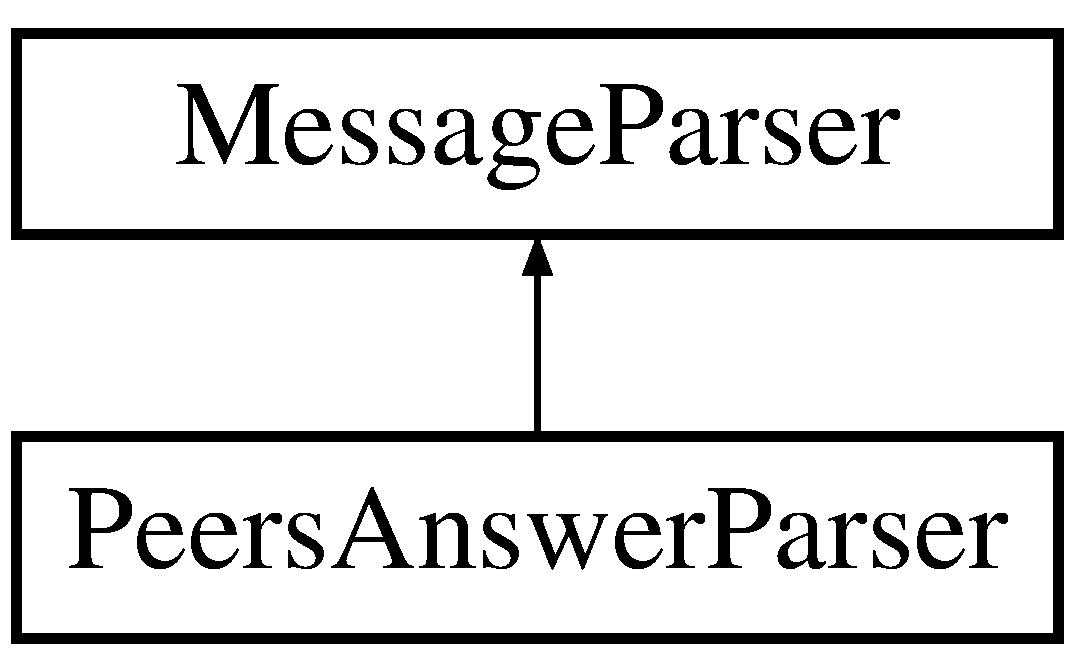
\includegraphics[height=2.000000cm]{classPeersAnswerParser}
\end{center}
\end{figure}
\subsection*{Public Member Functions}
\begin{DoxyCompactItemize}
\item 
void \mbox{\hyperlink{classPeersAnswerParser_ad566095c0594805919e7e4d14f8b076e}{operator()}} (\mbox{\hyperlink{classMessage}{Message}} $\ast$m, \mbox{\hyperlink{classNode}{Node}} $\ast$node) const final
\item 
int \mbox{\hyperlink{classPeersAnswerParser_a5f88ed07616ae3d17726f27b263645a6}{get\+\_\+type}} () const final
\end{DoxyCompactItemize}


\subsection{Detailed Description}
A message parser linked to a \mbox{\hyperlink{classAnswerPeersMessage}{Answer\+Peers\+Message}}. \begin{DoxySeeAlso}{See also}
\mbox{\hyperlink{classMessage}{Message}} 

\mbox{\hyperlink{classAnswerPeersMessage}{Answer\+Peers\+Message}} 

\mbox{\hyperlink{classMessageParser}{Message\+Parser}}
\end{DoxySeeAlso}
\begin{DoxyAuthor}{Author}
Mathieu Lochet 
\end{DoxyAuthor}
\begin{DoxyVersion}{Version}
1 
\end{DoxyVersion}


\subsection{Member Function Documentation}
\mbox{\Hypertarget{classPeersAnswerParser_a5f88ed07616ae3d17726f27b263645a6}\label{classPeersAnswerParser_a5f88ed07616ae3d17726f27b263645a6}} 
\index{Peers\+Answer\+Parser@{Peers\+Answer\+Parser}!get\+\_\+type@{get\+\_\+type}}
\index{get\+\_\+type@{get\+\_\+type}!Peers\+Answer\+Parser@{Peers\+Answer\+Parser}}
\subsubsection{\texorpdfstring{get\+\_\+type()}{get\_type()}}
{\footnotesize\ttfamily int Peers\+Answer\+Parser\+::get\+\_\+type (\begin{DoxyParamCaption}{ }\end{DoxyParamCaption}) const\hspace{0.3cm}{\ttfamily [final]}, {\ttfamily [virtual]}}

Get the type of message the parser is linked to \begin{DoxySeeAlso}{See also}
\mbox{\hyperlink{classMessage}{Message}} 
\end{DoxySeeAlso}


Implements \mbox{\hyperlink{classMessageParser_aa7c495d7b28a394e5752ca25ffff69d8}{Message\+Parser}}.

\mbox{\Hypertarget{classPeersAnswerParser_ad566095c0594805919e7e4d14f8b076e}\label{classPeersAnswerParser_ad566095c0594805919e7e4d14f8b076e}} 
\index{Peers\+Answer\+Parser@{Peers\+Answer\+Parser}!operator()@{operator()}}
\index{operator()@{operator()}!Peers\+Answer\+Parser@{Peers\+Answer\+Parser}}
\subsubsection{\texorpdfstring{operator()()}{operator()()}}
{\footnotesize\ttfamily void Peers\+Answer\+Parser\+::operator() (\begin{DoxyParamCaption}\item[{\mbox{\hyperlink{classMessage}{Message}} $\ast$}]{m,  }\item[{\mbox{\hyperlink{classNode}{Node}} $\ast$}]{node }\end{DoxyParamCaption}) const\hspace{0.3cm}{\ttfamily [final]}, {\ttfamily [virtual]}}

Process the message \begin{DoxySeeAlso}{See also}
\mbox{\hyperlink{classMessage}{Message}} 

\mbox{\hyperlink{classNode}{Node}}
\end{DoxySeeAlso}

\begin{DoxyParams}{Parameters}
{\em m} & The received message \\
\hline
{\em node} & The peer receiving the message \\
\hline
\end{DoxyParams}


Implements \mbox{\hyperlink{classMessageParser_a946f3b936dc01a75d6165329b159ecfe}{Message\+Parser}}.



The documentation for this class was generated from the following files\+:\begin{DoxyCompactItemize}
\item 
block\+\_\+chain/kernel/parsers/Peers\+Answer\+Parser.\+h\item 
block\+\_\+chain/kernel/parsers/Peers\+Answer\+Parser.\+cpp\end{DoxyCompactItemize}

\hypertarget{classPeersAskParser}{}\section{Peers\+Ask\+Parser Class Reference}
\label{classPeersAskParser}\index{Peers\+Ask\+Parser@{Peers\+Ask\+Parser}}
Inheritance diagram for Peers\+Ask\+Parser\+:\begin{figure}[H]
\begin{center}
\leavevmode
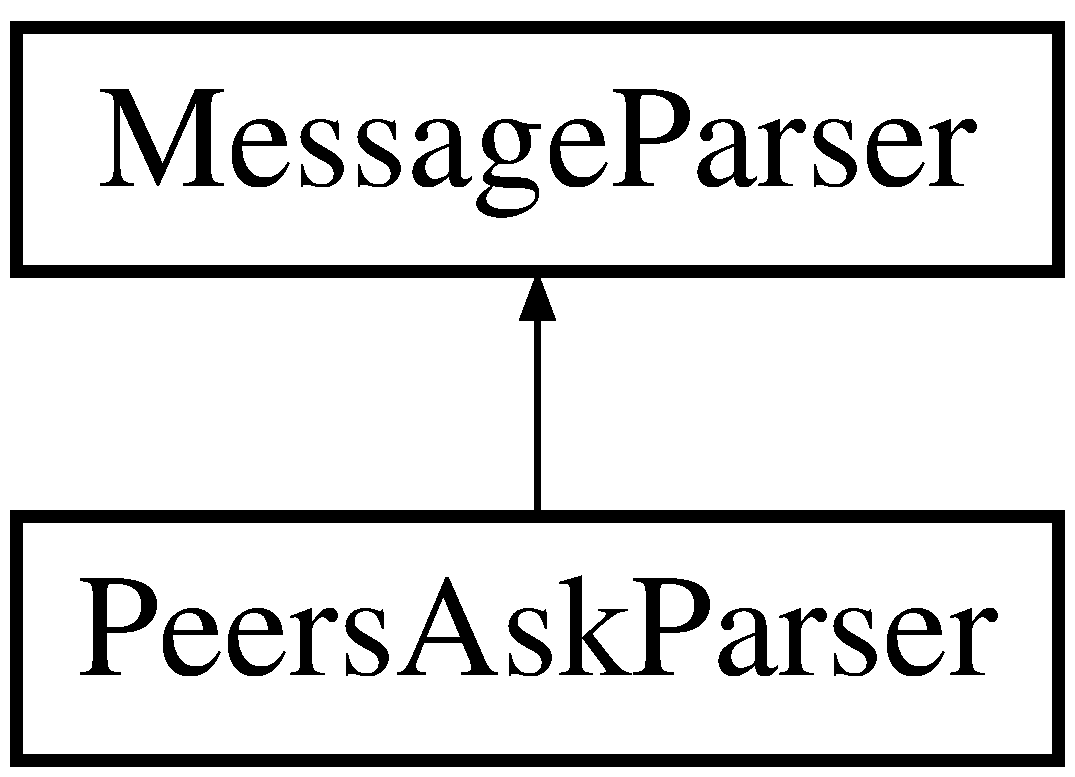
\includegraphics[height=2.000000cm]{classPeersAskParser}
\end{center}
\end{figure}
\subsection*{Public Member Functions}
\begin{DoxyCompactItemize}
\item 
\mbox{\Hypertarget{classPeersAskParser_ac52c9f42fa449029d49faaf9255b2d0d}\label{classPeersAskParser_ac52c9f42fa449029d49faaf9255b2d0d}} 
void {\bfseries operator()} (\mbox{\hyperlink{classMessage}{Message}} $\ast$m, \mbox{\hyperlink{classNode}{Node}} $\ast$node) const final
\item 
\mbox{\Hypertarget{classPeersAskParser_abda1a00fdca208592d3f7e7b039f9ba7}\label{classPeersAskParser_abda1a00fdca208592d3f7e7b039f9ba7}} 
int {\bfseries get\+\_\+type} () const final
\end{DoxyCompactItemize}


The documentation for this class was generated from the following files\+:\begin{DoxyCompactItemize}
\item 
block\+\_\+chain/kernel/parsers/Peers\+Ask\+Parser.\+h\item 
block\+\_\+chain/kernel/parsers/Peers\+Ask\+Parser.\+cpp\end{DoxyCompactItemize}

\hypertarget{classProof}{}\section{Proof Class Reference}
\label{classProof}\index{Proof@{Proof}}


{\ttfamily \#include $<$Proof.\+h$>$}

Inheritance diagram for Proof\+:\begin{figure}[H]
\begin{center}
\leavevmode
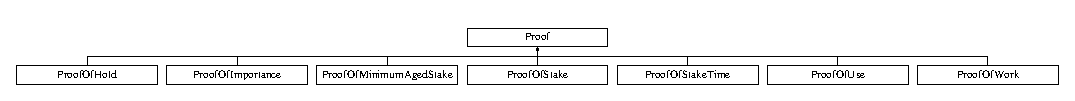
\includegraphics[height=0.914286cm]{classProof}
\end{center}
\end{figure}
\subsection*{Public Member Functions}
\begin{DoxyCompactItemize}
\item 
virtual void \mbox{\hyperlink{classProof_a6ab9f6c3f603447e3a9c7c932b5deac4}{run}} (\mbox{\hyperlink{classBlock}{Block}} $\ast$block, std\+::string key) const =0
\item 
virtual bool \mbox{\hyperlink{classProof_a358b3883eb33b8ecc93f74cb6313679a}{accept}} (\mbox{\hyperlink{classBlock}{Block}} $\ast$block, \mbox{\hyperlink{classMessage}{Message}} $\ast$) const =0
\item 
virtual \mbox{\hyperlink{classProof_a7d4b4e1b7e891dc1d437ef4095f778df}{$\sim$\+Proof}} ()=default
\end{DoxyCompactItemize}
\subsection*{Static Public Member Functions}
\begin{DoxyCompactItemize}
\item 
static void \mbox{\hyperlink{classProof_a71874539fdbcc93c15594b889c95225b}{add\+\_\+proof}} (int id, std\+::function$<$ \mbox{\hyperlink{classProof}{Proof}} $\ast$()$>$ proof)
\item 
static \mbox{\hyperlink{classProof}{Proof}} $\ast$ \mbox{\hyperlink{classProof_a267f0f4587babb59884b5f280e2d54c8}{generate}} (int type)
\end{DoxyCompactItemize}
\subsection*{Static Public Attributes}
\begin{DoxyCompactItemize}
\item 
\mbox{\Hypertarget{classProof_a457d231986439ee6bcc945daacfc28fc}\label{classProof_a457d231986439ee6bcc945daacfc28fc}} 
static const int {\bfseries W\+O\+RK} = 0
\item 
\mbox{\Hypertarget{classProof_acf157976c3c86ef2fd0e838b8c4ac992}\label{classProof_acf157976c3c86ef2fd0e838b8c4ac992}} 
static const int {\bfseries S\+T\+A\+KE} = 1
\item 
\mbox{\Hypertarget{classProof_ae5c2a86640bf558ff5625157e23b3eec}\label{classProof_ae5c2a86640bf558ff5625157e23b3eec}} 
static const int {\bfseries H\+O\+LD} = 2
\item 
\mbox{\Hypertarget{classProof_a4e71a5e5928900794353acdd169ca652}\label{classProof_a4e71a5e5928900794353acdd169ca652}} 
static const int {\bfseries I\+M\+P\+O\+R\+T\+A\+N\+CE} = 3
\item 
\mbox{\Hypertarget{classProof_a1a08ffc465f4fcfde396d4c4feb22eb0}\label{classProof_a1a08ffc465f4fcfde396d4c4feb22eb0}} 
static const int {\bfseries M\+I\+N\+I\+M\+U\+M\+\_\+\+A\+G\+E\+D\+\_\+\+S\+T\+A\+KE} = 4
\item 
\mbox{\Hypertarget{classProof_a1aa2cb91c5be4ca021714ff6fc01da4a}\label{classProof_a1aa2cb91c5be4ca021714ff6fc01da4a}} 
static const int {\bfseries S\+T\+A\+K\+E\+\_\+\+T\+I\+ME} = 5
\item 
\mbox{\Hypertarget{classProof_a3f6898fa1d652d32182c3c387c8e979c}\label{classProof_a3f6898fa1d652d32182c3c387c8e979c}} 
static const int {\bfseries U\+SE} = 6
\end{DoxyCompactItemize}


\subsection{Detailed Description}
An abstract proof and a proof factory. A proof is used to avoid falsification of the block chain Some proofs are provided and a user can create its own proofs and add them into the factory.

\begin{DoxyAuthor}{Author}
Mathieu Lochet 
\end{DoxyAuthor}
\begin{DoxyVersion}{Version}
1 
\end{DoxyVersion}


\subsection{Constructor \& Destructor Documentation}
\mbox{\Hypertarget{classProof_a7d4b4e1b7e891dc1d437ef4095f778df}\label{classProof_a7d4b4e1b7e891dc1d437ef4095f778df}} 
\index{Proof@{Proof}!````~Proof@{$\sim$\+Proof}}
\index{````~Proof@{$\sim$\+Proof}!Proof@{Proof}}
\subsubsection{\texorpdfstring{$\sim$\+Proof()}{~Proof()}}
{\footnotesize\ttfamily virtual Proof\+::$\sim$\+Proof (\begin{DoxyParamCaption}{ }\end{DoxyParamCaption})\hspace{0.3cm}{\ttfamily [virtual]}, {\ttfamily [default]}}

Default destructor 

\subsection{Member Function Documentation}
\mbox{\Hypertarget{classProof_a358b3883eb33b8ecc93f74cb6313679a}\label{classProof_a358b3883eb33b8ecc93f74cb6313679a}} 
\index{Proof@{Proof}!accept@{accept}}
\index{accept@{accept}!Proof@{Proof}}
\subsubsection{\texorpdfstring{accept()}{accept()}}
{\footnotesize\ttfamily virtual bool Proof\+::accept (\begin{DoxyParamCaption}\item[{\mbox{\hyperlink{classBlock}{Block}} $\ast$}]{block,  }\item[{\mbox{\hyperlink{classMessage}{Message}} $\ast$}]{ }\end{DoxyParamCaption}) const\hspace{0.3cm}{\ttfamily [pure virtual]}}

Get a proof result and check if the result is correct Needs to be implemented


\begin{DoxyParams}{Parameters}
{\em block} & The block to check the proof \\
\hline
{\em The} & received message \\
\hline
\end{DoxyParams}


Implemented in \mbox{\hyperlink{classProofOfHold_a4aa0ee52c0a6dcac18ab5ed84aae92e1}{Proof\+Of\+Hold}}, \mbox{\hyperlink{classProofOfImportance_a42a29f16c0c9e5e097fd734b7ee3fcf8}{Proof\+Of\+Importance}}, \mbox{\hyperlink{classProofOfMinimumAgedStake_aa42f7b715bb986143b5dda841782745b}{Proof\+Of\+Minimum\+Aged\+Stake}}, \mbox{\hyperlink{classProofOfStake_a5ee2b37cb25c63e1baa5c5b04e2dfca2}{Proof\+Of\+Stake}}, \mbox{\hyperlink{classProofOfStakeTime_ae05431416e9157fb8af8247b8e756794}{Proof\+Of\+Stake\+Time}}, \mbox{\hyperlink{classProofOfUse_a315614eb2b05b40367bdc11e60b7b8be}{Proof\+Of\+Use}}, and \mbox{\hyperlink{classProofOfWork_aa414484a6dc03fec583996a591f36856}{Proof\+Of\+Work}}.

\mbox{\Hypertarget{classProof_a71874539fdbcc93c15594b889c95225b}\label{classProof_a71874539fdbcc93c15594b889c95225b}} 
\index{Proof@{Proof}!add\+\_\+proof@{add\+\_\+proof}}
\index{add\+\_\+proof@{add\+\_\+proof}!Proof@{Proof}}
\subsubsection{\texorpdfstring{add\+\_\+proof()}{add\_proof()}}
{\footnotesize\ttfamily void Proof\+::add\+\_\+proof (\begin{DoxyParamCaption}\item[{int}]{id,  }\item[{std\+::function$<$ \mbox{\hyperlink{classProof}{Proof}} $\ast$()$>$}]{proof }\end{DoxyParamCaption})\hspace{0.3cm}{\ttfamily [static]}}

Allows the user to add its own proof into the system He the proof id is required


\begin{DoxyParams}{Parameters}
{\em id} & The proof id \\
\hline
{\em proof} & The lambda expression that creates a proof \\
\hline
\end{DoxyParams}
\mbox{\Hypertarget{classProof_a267f0f4587babb59884b5f280e2d54c8}\label{classProof_a267f0f4587babb59884b5f280e2d54c8}} 
\index{Proof@{Proof}!generate@{generate}}
\index{generate@{generate}!Proof@{Proof}}
\subsubsection{\texorpdfstring{generate()}{generate()}}
{\footnotesize\ttfamily \mbox{\hyperlink{classProof}{Proof}} $\ast$ Proof\+::generate (\begin{DoxyParamCaption}\item[{int}]{type }\end{DoxyParamCaption})\hspace{0.3cm}{\ttfamily [static]}}

Generates a proof for a given id


\begin{DoxyParams}{Parameters}
{\em id} & The proof id \\
\hline
\end{DoxyParams}
\begin{DoxyReturn}{Returns}
The created proof object 
\end{DoxyReturn}
\mbox{\Hypertarget{classProof_a6ab9f6c3f603447e3a9c7c932b5deac4}\label{classProof_a6ab9f6c3f603447e3a9c7c932b5deac4}} 
\index{Proof@{Proof}!run@{run}}
\index{run@{run}!Proof@{Proof}}
\subsubsection{\texorpdfstring{run()}{run()}}
{\footnotesize\ttfamily virtual void Proof\+::run (\begin{DoxyParamCaption}\item[{\mbox{\hyperlink{classBlock}{Block}} $\ast$}]{block,  }\item[{std\+::string}]{key }\end{DoxyParamCaption}) const\hspace{0.3cm}{\ttfamily [pure virtual]}}

Run a proof on a block to validate it Needs to be implemented


\begin{DoxyParams}{Parameters}
{\em block} & The block to run the proof on \\
\hline
{\em The} & user\textquotesingle{}s key to use in the process \\
\hline
\end{DoxyParams}


Implemented in \mbox{\hyperlink{classProofOfHold_a3daccb372774a6b4f6ed758be624eaf2}{Proof\+Of\+Hold}}, \mbox{\hyperlink{classProofOfImportance_a08f72d852cefc73c21bc22cbdaf956ff}{Proof\+Of\+Importance}}, \mbox{\hyperlink{classProofOfMinimumAgedStake_aab3c754b7bc7c1c1e2ccebdaa764249b}{Proof\+Of\+Minimum\+Aged\+Stake}}, \mbox{\hyperlink{classProofOfStake_ab5062d721fffffadfd9a599496d939dd}{Proof\+Of\+Stake}}, \mbox{\hyperlink{classProofOfStakeTime_a4081abb2bc76f8039995a73e9617086c}{Proof\+Of\+Stake\+Time}}, \mbox{\hyperlink{classProofOfUse_aefccdad0aa3344b6331acecc05299cc0}{Proof\+Of\+Use}}, and \mbox{\hyperlink{classProofOfWork_a31d9107577bafc58c5ce2374e79f2b3c}{Proof\+Of\+Work}}.



The documentation for this class was generated from the following files\+:\begin{DoxyCompactItemize}
\item 
block\+\_\+chain/chain/block/proof/Proof.\+h\item 
block\+\_\+chain/chain/block/proof/Proof.\+cpp\end{DoxyCompactItemize}

\hypertarget{classProofOfHold}{}\section{Proof\+Of\+Hold Class Reference}
\label{classProofOfHold}\index{Proof\+Of\+Hold@{Proof\+Of\+Hold}}


{\ttfamily \#include $<$Proof\+Of\+Hold.\+h$>$}

Inheritance diagram for Proof\+Of\+Hold\+:\begin{figure}[H]
\begin{center}
\leavevmode
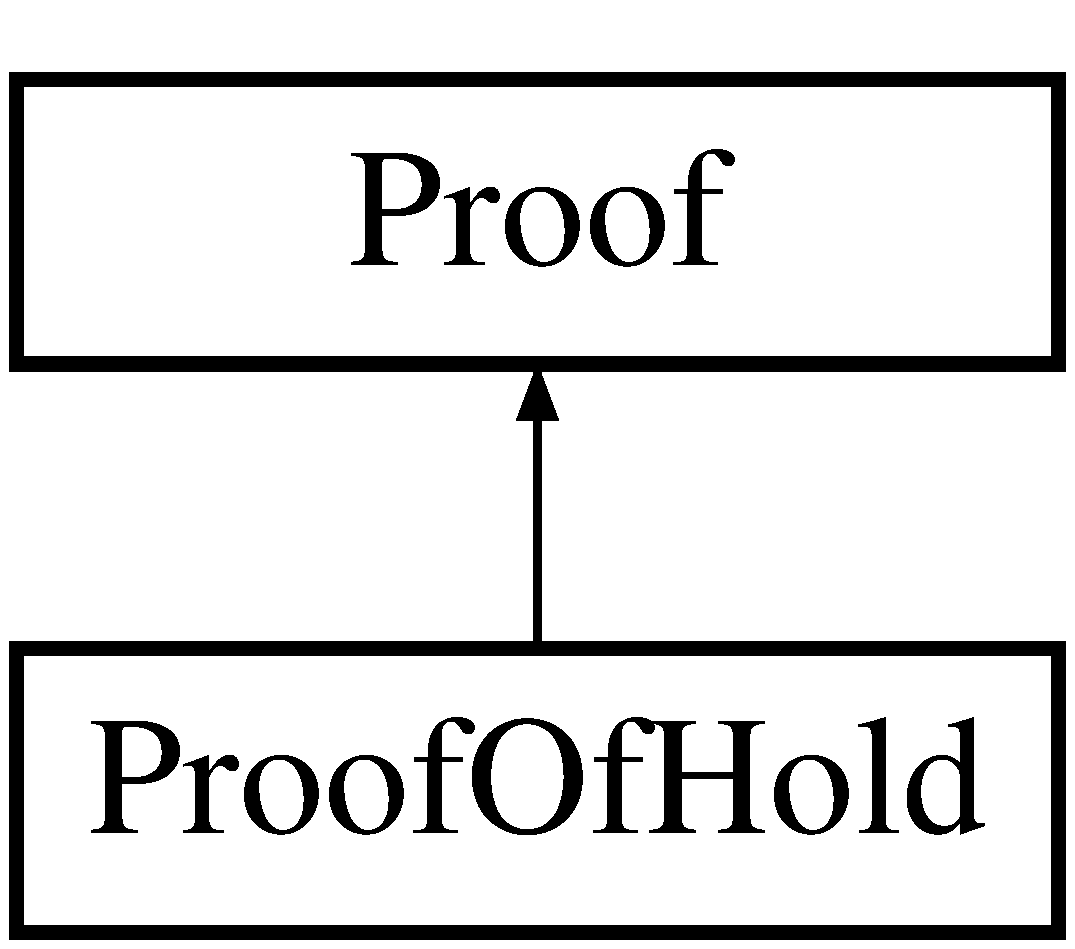
\includegraphics[height=2.000000cm]{classProofOfHold}
\end{center}
\end{figure}
\subsection*{Public Member Functions}
\begin{DoxyCompactItemize}
\item 
void \mbox{\hyperlink{classProofOfHold_a3daccb372774a6b4f6ed758be624eaf2}{run}} (\mbox{\hyperlink{classBlock}{Block}} $\ast$block, std\+::string key) const override
\item 
bool \mbox{\hyperlink{classProofOfHold_a4aa0ee52c0a6dcac18ab5ed84aae92e1}{accept}} (\mbox{\hyperlink{classBlock}{Block}} $\ast$block, \mbox{\hyperlink{classMessage}{Message}} $\ast$message) const override
\end{DoxyCompactItemize}
\subsection*{Static Public Member Functions}
\begin{DoxyCompactItemize}
\item 
static void \mbox{\hyperlink{classProof_a71874539fdbcc93c15594b889c95225b}{add\+\_\+proof}} (int id, std\+::function$<$ \mbox{\hyperlink{classProof}{Proof}} $\ast$()$>$ proof)
\item 
static \mbox{\hyperlink{classProof}{Proof}} $\ast$ \mbox{\hyperlink{classProof_a267f0f4587babb59884b5f280e2d54c8}{generate}} (int type)
\end{DoxyCompactItemize}
\subsection*{Static Public Attributes}
\begin{DoxyCompactItemize}
\item 
\mbox{\Hypertarget{classProof_a457d231986439ee6bcc945daacfc28fc}\label{classProof_a457d231986439ee6bcc945daacfc28fc}} 
static const int {\bfseries W\+O\+RK} = 0
\item 
\mbox{\Hypertarget{classProof_acf157976c3c86ef2fd0e838b8c4ac992}\label{classProof_acf157976c3c86ef2fd0e838b8c4ac992}} 
static const int {\bfseries S\+T\+A\+KE} = 1
\item 
\mbox{\Hypertarget{classProof_ae5c2a86640bf558ff5625157e23b3eec}\label{classProof_ae5c2a86640bf558ff5625157e23b3eec}} 
static const int {\bfseries H\+O\+LD} = 2
\item 
\mbox{\Hypertarget{classProof_a4e71a5e5928900794353acdd169ca652}\label{classProof_a4e71a5e5928900794353acdd169ca652}} 
static const int {\bfseries I\+M\+P\+O\+R\+T\+A\+N\+CE} = 3
\item 
\mbox{\Hypertarget{classProof_a1a08ffc465f4fcfde396d4c4feb22eb0}\label{classProof_a1a08ffc465f4fcfde396d4c4feb22eb0}} 
static const int {\bfseries M\+I\+N\+I\+M\+U\+M\+\_\+\+A\+G\+E\+D\+\_\+\+S\+T\+A\+KE} = 4
\item 
\mbox{\Hypertarget{classProof_a1aa2cb91c5be4ca021714ff6fc01da4a}\label{classProof_a1aa2cb91c5be4ca021714ff6fc01da4a}} 
static const int {\bfseries S\+T\+A\+K\+E\+\_\+\+T\+I\+ME} = 5
\item 
\mbox{\Hypertarget{classProof_a3f6898fa1d652d32182c3c387c8e979c}\label{classProof_a3f6898fa1d652d32182c3c387c8e979c}} 
static const int {\bfseries U\+SE} = 6
\end{DoxyCompactItemize}


\subsection{Detailed Description}
A basic proof of hold \begin{DoxySeeAlso}{See also}
\mbox{\hyperlink{classProof}{Proof}} 

Proof\+::\+H\+O\+LD
\end{DoxySeeAlso}
\begin{DoxyAuthor}{Author}
Mathieu Lochet 
\end{DoxyAuthor}
\begin{DoxyVersion}{Version}
1 
\end{DoxyVersion}


\subsection{Member Function Documentation}
\mbox{\Hypertarget{classProofOfHold_a4aa0ee52c0a6dcac18ab5ed84aae92e1}\label{classProofOfHold_a4aa0ee52c0a6dcac18ab5ed84aae92e1}} 
\index{Proof\+Of\+Hold@{Proof\+Of\+Hold}!accept@{accept}}
\index{accept@{accept}!Proof\+Of\+Hold@{Proof\+Of\+Hold}}
\subsubsection{\texorpdfstring{accept()}{accept()}}
{\footnotesize\ttfamily bool Proof\+Of\+Hold\+::accept (\begin{DoxyParamCaption}\item[{\mbox{\hyperlink{classBlock}{Block}} $\ast$}]{block,  }\item[{\mbox{\hyperlink{classMessage}{Message}} $\ast$}]{ }\end{DoxyParamCaption}) const\hspace{0.3cm}{\ttfamily [override]}, {\ttfamily [virtual]}}

Get a proof result and check if the result is correct Needs to be implemented


\begin{DoxyParams}{Parameters}
{\em block} & The block to check the proof \\
\hline
{\em The} & received message \\
\hline
\end{DoxyParams}


Implements \mbox{\hyperlink{classProof_a358b3883eb33b8ecc93f74cb6313679a}{Proof}}.

\mbox{\Hypertarget{classProof_a71874539fdbcc93c15594b889c95225b}\label{classProof_a71874539fdbcc93c15594b889c95225b}} 
\index{Proof\+Of\+Hold@{Proof\+Of\+Hold}!add\+\_\+proof@{add\+\_\+proof}}
\index{add\+\_\+proof@{add\+\_\+proof}!Proof\+Of\+Hold@{Proof\+Of\+Hold}}
\subsubsection{\texorpdfstring{add\+\_\+proof()}{add\_proof()}}
{\footnotesize\ttfamily void Proof\+::add\+\_\+proof (\begin{DoxyParamCaption}\item[{int}]{id,  }\item[{std\+::function$<$ \mbox{\hyperlink{classProof}{Proof}} $\ast$()$>$}]{proof }\end{DoxyParamCaption})\hspace{0.3cm}{\ttfamily [static]}, {\ttfamily [inherited]}}

Allows the user to add its own proof into the system He the proof id is required


\begin{DoxyParams}{Parameters}
{\em id} & The proof id \\
\hline
{\em proof} & The lambda expression that creates a proof \\
\hline
\end{DoxyParams}
\mbox{\Hypertarget{classProof_a267f0f4587babb59884b5f280e2d54c8}\label{classProof_a267f0f4587babb59884b5f280e2d54c8}} 
\index{Proof\+Of\+Hold@{Proof\+Of\+Hold}!generate@{generate}}
\index{generate@{generate}!Proof\+Of\+Hold@{Proof\+Of\+Hold}}
\subsubsection{\texorpdfstring{generate()}{generate()}}
{\footnotesize\ttfamily \mbox{\hyperlink{classProof}{Proof}} $\ast$ Proof\+::generate (\begin{DoxyParamCaption}\item[{int}]{type }\end{DoxyParamCaption})\hspace{0.3cm}{\ttfamily [static]}, {\ttfamily [inherited]}}

Generates a proof for a given id


\begin{DoxyParams}{Parameters}
{\em id} & The proof id \\
\hline
\end{DoxyParams}
\begin{DoxyReturn}{Returns}
The created proof object 
\end{DoxyReturn}
\mbox{\Hypertarget{classProofOfHold_a3daccb372774a6b4f6ed758be624eaf2}\label{classProofOfHold_a3daccb372774a6b4f6ed758be624eaf2}} 
\index{Proof\+Of\+Hold@{Proof\+Of\+Hold}!run@{run}}
\index{run@{run}!Proof\+Of\+Hold@{Proof\+Of\+Hold}}
\subsubsection{\texorpdfstring{run()}{run()}}
{\footnotesize\ttfamily void Proof\+Of\+Hold\+::run (\begin{DoxyParamCaption}\item[{\mbox{\hyperlink{classBlock}{Block}} $\ast$}]{block,  }\item[{std\+::string}]{key }\end{DoxyParamCaption}) const\hspace{0.3cm}{\ttfamily [override]}, {\ttfamily [virtual]}}

Run a proof on a block to validate it Needs to be implemented


\begin{DoxyParams}{Parameters}
{\em block} & The block to run the proof on \\
\hline
{\em The} & user\textquotesingle{}s key to use in the process \\
\hline
\end{DoxyParams}


Implements \mbox{\hyperlink{classProof_a6ab9f6c3f603447e3a9c7c932b5deac4}{Proof}}.



The documentation for this class was generated from the following files\+:\begin{DoxyCompactItemize}
\item 
block\+\_\+chain/chain/block/proof/Proof\+Of\+Hold.\+h\item 
block\+\_\+chain/chain/block/proof/Proof\+Of\+Hold.\+cpp\end{DoxyCompactItemize}

\hypertarget{classProofOfImportance}{}\section{Proof\+Of\+Importance Class Reference}
\label{classProofOfImportance}\index{Proof\+Of\+Importance@{Proof\+Of\+Importance}}
Inheritance diagram for Proof\+Of\+Importance\+:\begin{figure}[H]
\begin{center}
\leavevmode
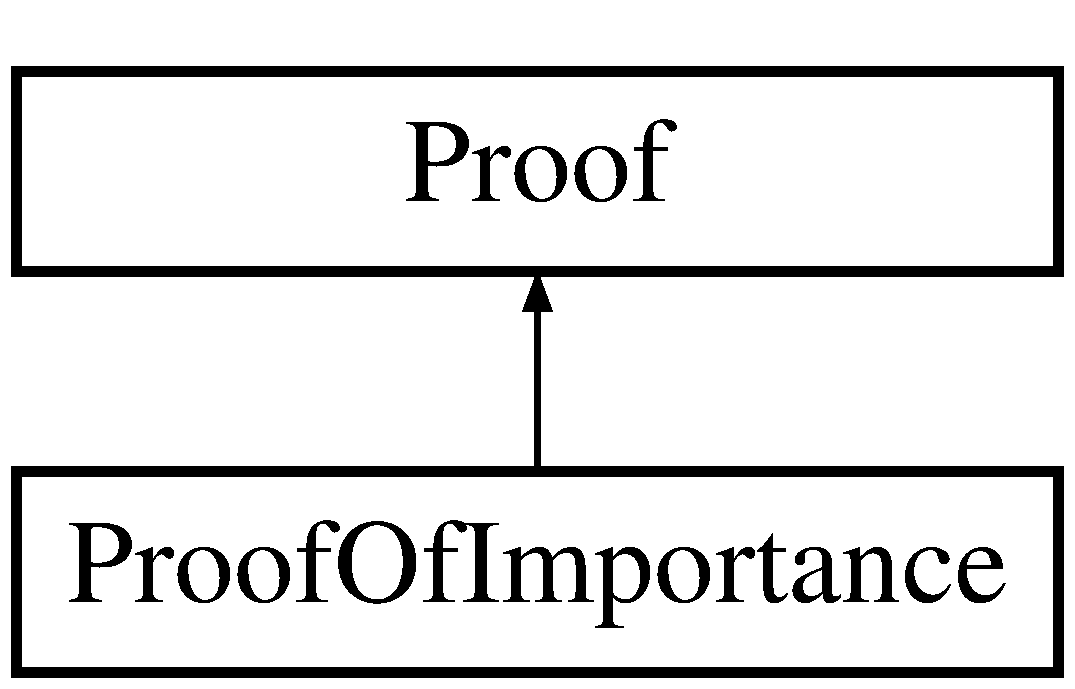
\includegraphics[height=2.000000cm]{classProofOfImportance}
\end{center}
\end{figure}
\subsection*{Public Member Functions}
\begin{DoxyCompactItemize}
\item 
\mbox{\Hypertarget{classProofOfImportance_afb53c930bf8afc5371ae91da04927415}\label{classProofOfImportance_afb53c930bf8afc5371ae91da04927415}} 
void {\bfseries run} (\mbox{\hyperlink{classBlock}{Block}} $\ast$block, std\+::string key) override
\item 
\mbox{\Hypertarget{classProofOfImportance_ab40da85ecfe7b87f21c63641d255f94e}\label{classProofOfImportance_ab40da85ecfe7b87f21c63641d255f94e}} 
bool {\bfseries accept} (\mbox{\hyperlink{classBlock}{Block}} $\ast$block, \mbox{\hyperlink{classMessage}{Message}} $\ast$message) override
\end{DoxyCompactItemize}
\subsection*{Static Public Member Functions}
\begin{DoxyCompactItemize}
\item 
\mbox{\Hypertarget{classProof_a93208e5161d25f8533849ac2dac8d6b8}\label{classProof_a93208e5161d25f8533849ac2dac8d6b8}} 
static void {\bfseries add\+\_\+proof} (int id, std\+::function$<$ \mbox{\hyperlink{classProof}{Proof}} $\ast$()$>$)
\item 
\mbox{\Hypertarget{classProof_a267f0f4587babb59884b5f280e2d54c8}\label{classProof_a267f0f4587babb59884b5f280e2d54c8}} 
static \mbox{\hyperlink{classProof}{Proof}} $\ast$ {\bfseries generate} (int type)
\end{DoxyCompactItemize}
\subsection*{Static Public Attributes}
\begin{DoxyCompactItemize}
\item 
\mbox{\Hypertarget{classProof_a457d231986439ee6bcc945daacfc28fc}\label{classProof_a457d231986439ee6bcc945daacfc28fc}} 
static const int {\bfseries W\+O\+RK} = 0
\item 
\mbox{\Hypertarget{classProof_acf157976c3c86ef2fd0e838b8c4ac992}\label{classProof_acf157976c3c86ef2fd0e838b8c4ac992}} 
static const int {\bfseries S\+T\+A\+KE} = 1
\item 
\mbox{\Hypertarget{classProof_ae5c2a86640bf558ff5625157e23b3eec}\label{classProof_ae5c2a86640bf558ff5625157e23b3eec}} 
static const int {\bfseries H\+O\+LD} = 2
\item 
\mbox{\Hypertarget{classProof_a4e71a5e5928900794353acdd169ca652}\label{classProof_a4e71a5e5928900794353acdd169ca652}} 
static const int {\bfseries I\+M\+P\+O\+R\+T\+A\+N\+CE} = 3
\item 
\mbox{\Hypertarget{classProof_a1a08ffc465f4fcfde396d4c4feb22eb0}\label{classProof_a1a08ffc465f4fcfde396d4c4feb22eb0}} 
static const int {\bfseries M\+I\+N\+I\+M\+U\+M\+\_\+\+A\+G\+E\+D\+\_\+\+S\+T\+A\+KE} = 4
\item 
\mbox{\Hypertarget{classProof_a1aa2cb91c5be4ca021714ff6fc01da4a}\label{classProof_a1aa2cb91c5be4ca021714ff6fc01da4a}} 
static const int {\bfseries S\+T\+A\+K\+E\+\_\+\+T\+I\+ME} = 5
\item 
\mbox{\Hypertarget{classProof_a3f6898fa1d652d32182c3c387c8e979c}\label{classProof_a3f6898fa1d652d32182c3c387c8e979c}} 
static const int {\bfseries U\+SE} = 6
\end{DoxyCompactItemize}


The documentation for this class was generated from the following files\+:\begin{DoxyCompactItemize}
\item 
block\+\_\+chain/chain/block/proof/Proof\+Of\+Importance.\+h\item 
block\+\_\+chain/chain/block/proof/Proof\+Of\+Importance.\+cpp\end{DoxyCompactItemize}

\hypertarget{classProofOfMinimumAgedStake}{}\section{Proof\+Of\+Minimum\+Aged\+Stake Class Reference}
\label{classProofOfMinimumAgedStake}\index{Proof\+Of\+Minimum\+Aged\+Stake@{Proof\+Of\+Minimum\+Aged\+Stake}}
Inheritance diagram for Proof\+Of\+Minimum\+Aged\+Stake\+:\begin{figure}[H]
\begin{center}
\leavevmode
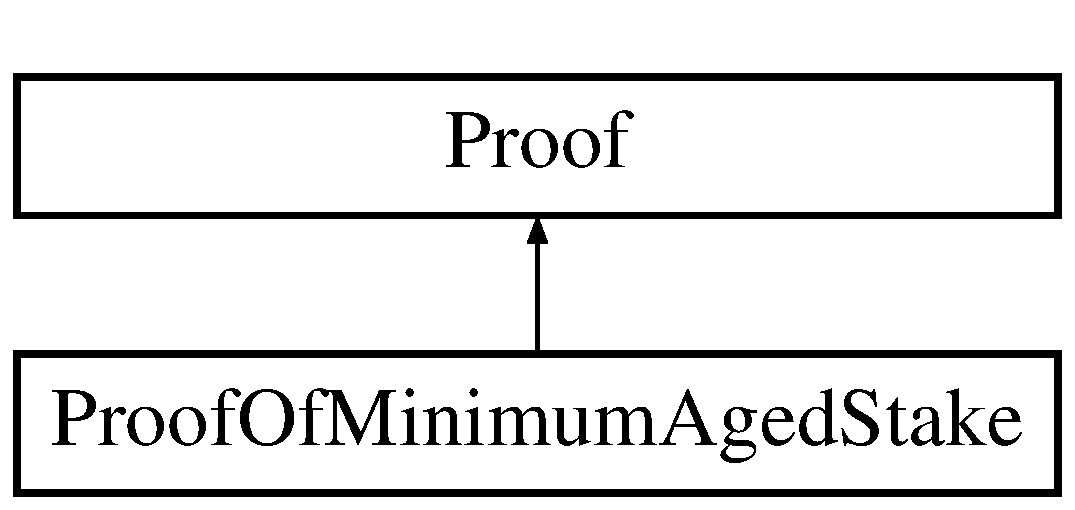
\includegraphics[height=2.000000cm]{classProofOfMinimumAgedStake}
\end{center}
\end{figure}
\subsection*{Public Member Functions}
\begin{DoxyCompactItemize}
\item 
\mbox{\Hypertarget{classProofOfMinimumAgedStake_aa850369d6f8ebf7fa833821a43049147}\label{classProofOfMinimumAgedStake_aa850369d6f8ebf7fa833821a43049147}} 
void {\bfseries run} (\mbox{\hyperlink{classBlock}{Block}} $\ast$block, std\+::string key) override
\item 
\mbox{\Hypertarget{classProofOfMinimumAgedStake_add68213606b37c50390cf1a0dd16c17b}\label{classProofOfMinimumAgedStake_add68213606b37c50390cf1a0dd16c17b}} 
bool {\bfseries accept} (\mbox{\hyperlink{classBlock}{Block}} $\ast$block, \mbox{\hyperlink{classMessage}{Message}} $\ast$message) override
\end{DoxyCompactItemize}
\subsection*{Static Public Member Functions}
\begin{DoxyCompactItemize}
\item 
\mbox{\Hypertarget{classProof_a93208e5161d25f8533849ac2dac8d6b8}\label{classProof_a93208e5161d25f8533849ac2dac8d6b8}} 
static void {\bfseries add\+\_\+proof} (int id, std\+::function$<$ \mbox{\hyperlink{classProof}{Proof}} $\ast$()$>$)
\item 
\mbox{\Hypertarget{classProof_a267f0f4587babb59884b5f280e2d54c8}\label{classProof_a267f0f4587babb59884b5f280e2d54c8}} 
static \mbox{\hyperlink{classProof}{Proof}} $\ast$ {\bfseries generate} (int type)
\end{DoxyCompactItemize}
\subsection*{Static Public Attributes}
\begin{DoxyCompactItemize}
\item 
\mbox{\Hypertarget{classProof_a457d231986439ee6bcc945daacfc28fc}\label{classProof_a457d231986439ee6bcc945daacfc28fc}} 
static const int {\bfseries W\+O\+RK} = 0
\item 
\mbox{\Hypertarget{classProof_acf157976c3c86ef2fd0e838b8c4ac992}\label{classProof_acf157976c3c86ef2fd0e838b8c4ac992}} 
static const int {\bfseries S\+T\+A\+KE} = 1
\item 
\mbox{\Hypertarget{classProof_ae5c2a86640bf558ff5625157e23b3eec}\label{classProof_ae5c2a86640bf558ff5625157e23b3eec}} 
static const int {\bfseries H\+O\+LD} = 2
\item 
\mbox{\Hypertarget{classProof_a4e71a5e5928900794353acdd169ca652}\label{classProof_a4e71a5e5928900794353acdd169ca652}} 
static const int {\bfseries I\+M\+P\+O\+R\+T\+A\+N\+CE} = 3
\item 
\mbox{\Hypertarget{classProof_a1a08ffc465f4fcfde396d4c4feb22eb0}\label{classProof_a1a08ffc465f4fcfde396d4c4feb22eb0}} 
static const int {\bfseries M\+I\+N\+I\+M\+U\+M\+\_\+\+A\+G\+E\+D\+\_\+\+S\+T\+A\+KE} = 4
\item 
\mbox{\Hypertarget{classProof_a1aa2cb91c5be4ca021714ff6fc01da4a}\label{classProof_a1aa2cb91c5be4ca021714ff6fc01da4a}} 
static const int {\bfseries S\+T\+A\+K\+E\+\_\+\+T\+I\+ME} = 5
\item 
\mbox{\Hypertarget{classProof_a3f6898fa1d652d32182c3c387c8e979c}\label{classProof_a3f6898fa1d652d32182c3c387c8e979c}} 
static const int {\bfseries U\+SE} = 6
\end{DoxyCompactItemize}


The documentation for this class was generated from the following files\+:\begin{DoxyCompactItemize}
\item 
block\+\_\+chain/chain/block/proof/Proof\+Of\+Minimum\+Aged\+Stake.\+h\item 
block\+\_\+chain/chain/block/proof/Proof\+Of\+Minimum\+Aged\+Stake.\+cpp\end{DoxyCompactItemize}

\hypertarget{classProofOfStake}{}\section{Proof\+Of\+Stake Class Reference}
\label{classProofOfStake}\index{Proof\+Of\+Stake@{Proof\+Of\+Stake}}


{\ttfamily \#include $<$Proof\+Of\+Stake.\+h$>$}

Inheritance diagram for Proof\+Of\+Stake\+:\begin{figure}[H]
\begin{center}
\leavevmode
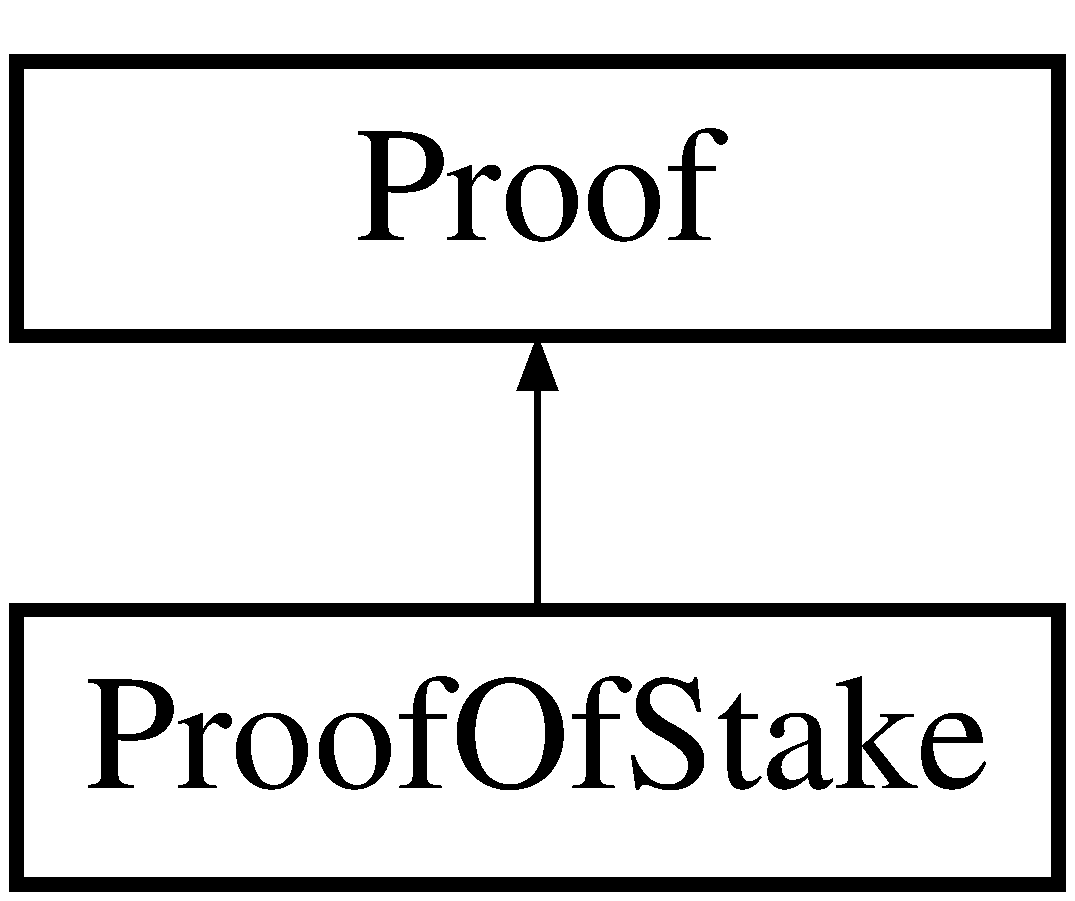
\includegraphics[height=2.000000cm]{classProofOfStake}
\end{center}
\end{figure}
\subsection*{Public Member Functions}
\begin{DoxyCompactItemize}
\item 
void \mbox{\hyperlink{classProofOfStake_ab5062d721fffffadfd9a599496d939dd}{run}} (\mbox{\hyperlink{classBlock}{Block}} $\ast$block, std\+::string key) const override
\item 
bool \mbox{\hyperlink{classProofOfStake_a5ee2b37cb25c63e1baa5c5b04e2dfca2}{accept}} (\mbox{\hyperlink{classBlock}{Block}} $\ast$block, \mbox{\hyperlink{classMessage}{Message}} $\ast$message) const override
\end{DoxyCompactItemize}
\subsection*{Static Public Member Functions}
\begin{DoxyCompactItemize}
\item 
static void \mbox{\hyperlink{classProof_a71874539fdbcc93c15594b889c95225b}{add\+\_\+proof}} (int id, std\+::function$<$ \mbox{\hyperlink{classProof}{Proof}} $\ast$()$>$ proof)
\item 
static \mbox{\hyperlink{classProof}{Proof}} $\ast$ \mbox{\hyperlink{classProof_a267f0f4587babb59884b5f280e2d54c8}{generate}} (int type)
\end{DoxyCompactItemize}
\subsection*{Static Public Attributes}
\begin{DoxyCompactItemize}
\item 
\mbox{\Hypertarget{classProof_a457d231986439ee6bcc945daacfc28fc}\label{classProof_a457d231986439ee6bcc945daacfc28fc}} 
static const int {\bfseries W\+O\+RK} = 0
\item 
\mbox{\Hypertarget{classProof_acf157976c3c86ef2fd0e838b8c4ac992}\label{classProof_acf157976c3c86ef2fd0e838b8c4ac992}} 
static const int {\bfseries S\+T\+A\+KE} = 1
\item 
\mbox{\Hypertarget{classProof_ae5c2a86640bf558ff5625157e23b3eec}\label{classProof_ae5c2a86640bf558ff5625157e23b3eec}} 
static const int {\bfseries H\+O\+LD} = 2
\item 
\mbox{\Hypertarget{classProof_a4e71a5e5928900794353acdd169ca652}\label{classProof_a4e71a5e5928900794353acdd169ca652}} 
static const int {\bfseries I\+M\+P\+O\+R\+T\+A\+N\+CE} = 3
\item 
\mbox{\Hypertarget{classProof_a1a08ffc465f4fcfde396d4c4feb22eb0}\label{classProof_a1a08ffc465f4fcfde396d4c4feb22eb0}} 
static const int {\bfseries M\+I\+N\+I\+M\+U\+M\+\_\+\+A\+G\+E\+D\+\_\+\+S\+T\+A\+KE} = 4
\item 
\mbox{\Hypertarget{classProof_a1aa2cb91c5be4ca021714ff6fc01da4a}\label{classProof_a1aa2cb91c5be4ca021714ff6fc01da4a}} 
static const int {\bfseries S\+T\+A\+K\+E\+\_\+\+T\+I\+ME} = 5
\item 
\mbox{\Hypertarget{classProof_a3f6898fa1d652d32182c3c387c8e979c}\label{classProof_a3f6898fa1d652d32182c3c387c8e979c}} 
static const int {\bfseries U\+SE} = 6
\end{DoxyCompactItemize}


\subsection{Detailed Description}
A basic proof of stake \begin{DoxySeeAlso}{See also}
\mbox{\hyperlink{classProof}{Proof}} 

Proof\+::\+S\+T\+A\+KE
\end{DoxySeeAlso}
\begin{DoxyAuthor}{Author}
Mathieu Lochet 
\end{DoxyAuthor}
\begin{DoxyVersion}{Version}
1 
\end{DoxyVersion}


\subsection{Member Function Documentation}
\mbox{\Hypertarget{classProofOfStake_a5ee2b37cb25c63e1baa5c5b04e2dfca2}\label{classProofOfStake_a5ee2b37cb25c63e1baa5c5b04e2dfca2}} 
\index{Proof\+Of\+Stake@{Proof\+Of\+Stake}!accept@{accept}}
\index{accept@{accept}!Proof\+Of\+Stake@{Proof\+Of\+Stake}}
\subsubsection{\texorpdfstring{accept()}{accept()}}
{\footnotesize\ttfamily bool Proof\+Of\+Stake\+::accept (\begin{DoxyParamCaption}\item[{\mbox{\hyperlink{classBlock}{Block}} $\ast$}]{block,  }\item[{\mbox{\hyperlink{classMessage}{Message}} $\ast$}]{ }\end{DoxyParamCaption}) const\hspace{0.3cm}{\ttfamily [override]}, {\ttfamily [virtual]}}

Get a proof result and check if the result is correct Needs to be implemented


\begin{DoxyParams}{Parameters}
{\em block} & The block to check the proof \\
\hline
{\em The} & received message \\
\hline
\end{DoxyParams}


Implements \mbox{\hyperlink{classProof_a358b3883eb33b8ecc93f74cb6313679a}{Proof}}.

\mbox{\Hypertarget{classProof_a71874539fdbcc93c15594b889c95225b}\label{classProof_a71874539fdbcc93c15594b889c95225b}} 
\index{Proof\+Of\+Stake@{Proof\+Of\+Stake}!add\+\_\+proof@{add\+\_\+proof}}
\index{add\+\_\+proof@{add\+\_\+proof}!Proof\+Of\+Stake@{Proof\+Of\+Stake}}
\subsubsection{\texorpdfstring{add\+\_\+proof()}{add\_proof()}}
{\footnotesize\ttfamily void Proof\+::add\+\_\+proof (\begin{DoxyParamCaption}\item[{int}]{id,  }\item[{std\+::function$<$ \mbox{\hyperlink{classProof}{Proof}} $\ast$()$>$}]{proof }\end{DoxyParamCaption})\hspace{0.3cm}{\ttfamily [static]}, {\ttfamily [inherited]}}

Allows the user to add its own proof into the system He the proof id is required


\begin{DoxyParams}{Parameters}
{\em id} & The proof id \\
\hline
{\em proof} & The lambda expression that creates a proof \\
\hline
\end{DoxyParams}
\mbox{\Hypertarget{classProof_a267f0f4587babb59884b5f280e2d54c8}\label{classProof_a267f0f4587babb59884b5f280e2d54c8}} 
\index{Proof\+Of\+Stake@{Proof\+Of\+Stake}!generate@{generate}}
\index{generate@{generate}!Proof\+Of\+Stake@{Proof\+Of\+Stake}}
\subsubsection{\texorpdfstring{generate()}{generate()}}
{\footnotesize\ttfamily \mbox{\hyperlink{classProof}{Proof}} $\ast$ Proof\+::generate (\begin{DoxyParamCaption}\item[{int}]{type }\end{DoxyParamCaption})\hspace{0.3cm}{\ttfamily [static]}, {\ttfamily [inherited]}}

Generates a proof for a given id


\begin{DoxyParams}{Parameters}
{\em id} & The proof id \\
\hline
\end{DoxyParams}
\begin{DoxyReturn}{Returns}
The created proof object 
\end{DoxyReturn}
\mbox{\Hypertarget{classProofOfStake_ab5062d721fffffadfd9a599496d939dd}\label{classProofOfStake_ab5062d721fffffadfd9a599496d939dd}} 
\index{Proof\+Of\+Stake@{Proof\+Of\+Stake}!run@{run}}
\index{run@{run}!Proof\+Of\+Stake@{Proof\+Of\+Stake}}
\subsubsection{\texorpdfstring{run()}{run()}}
{\footnotesize\ttfamily void Proof\+Of\+Stake\+::run (\begin{DoxyParamCaption}\item[{\mbox{\hyperlink{classBlock}{Block}} $\ast$}]{block,  }\item[{std\+::string}]{key }\end{DoxyParamCaption}) const\hspace{0.3cm}{\ttfamily [override]}, {\ttfamily [virtual]}}

Run a proof on a block to validate it Needs to be implemented


\begin{DoxyParams}{Parameters}
{\em block} & The block to run the proof on \\
\hline
{\em The} & user\textquotesingle{}s key to use in the process \\
\hline
\end{DoxyParams}


Implements \mbox{\hyperlink{classProof_a6ab9f6c3f603447e3a9c7c932b5deac4}{Proof}}.



The documentation for this class was generated from the following files\+:\begin{DoxyCompactItemize}
\item 
block\+\_\+chain/chain/block/proof/Proof\+Of\+Stake.\+h\item 
block\+\_\+chain/chain/block/proof/Proof\+Of\+Stake.\+cpp\end{DoxyCompactItemize}

\hypertarget{classProofOfStakeTime}{}\section{Proof\+Of\+Stake\+Time Class Reference}
\label{classProofOfStakeTime}\index{Proof\+Of\+Stake\+Time@{Proof\+Of\+Stake\+Time}}


{\ttfamily \#include $<$Proof\+Of\+Stake\+Time.\+h$>$}

Inheritance diagram for Proof\+Of\+Stake\+Time\+:\begin{figure}[H]
\begin{center}
\leavevmode
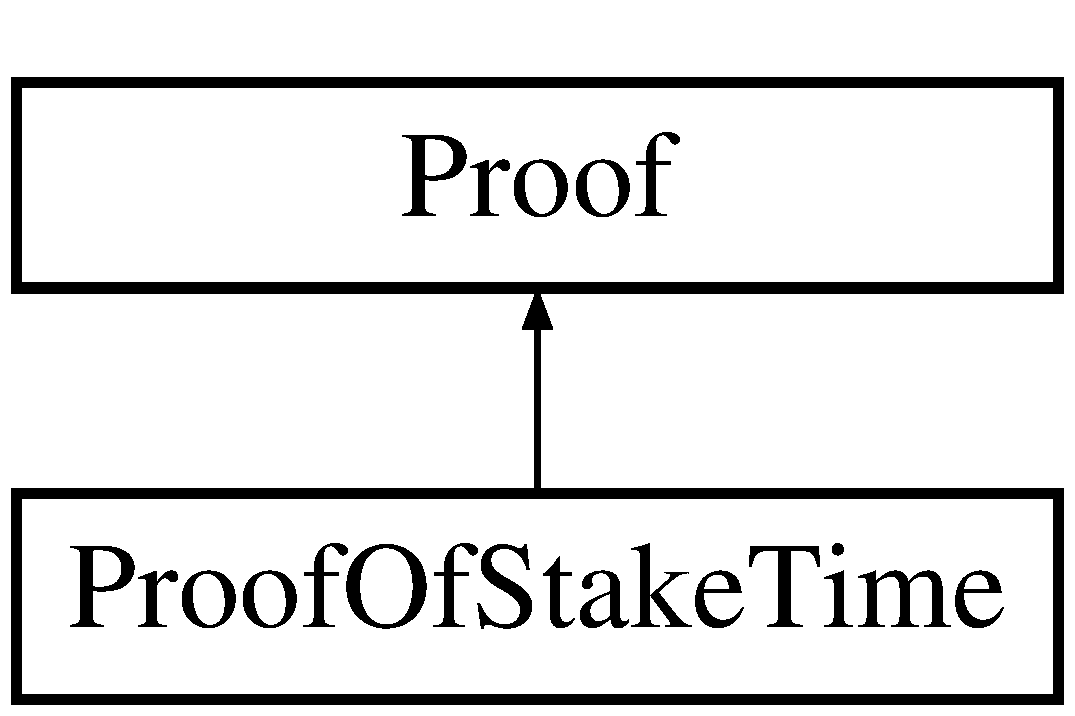
\includegraphics[height=2.000000cm]{classProofOfStakeTime}
\end{center}
\end{figure}
\subsection*{Public Member Functions}
\begin{DoxyCompactItemize}
\item 
void \mbox{\hyperlink{classProofOfStakeTime_a4081abb2bc76f8039995a73e9617086c}{run}} (\mbox{\hyperlink{classBlock}{Block}} $\ast$block, std\+::string key) const override
\item 
bool \mbox{\hyperlink{classProofOfStakeTime_ae05431416e9157fb8af8247b8e756794}{accept}} (\mbox{\hyperlink{classBlock}{Block}} $\ast$block, \mbox{\hyperlink{classMessage}{Message}} $\ast$message) const override
\end{DoxyCompactItemize}
\subsection*{Static Public Member Functions}
\begin{DoxyCompactItemize}
\item 
static void \mbox{\hyperlink{classProof_a71874539fdbcc93c15594b889c95225b}{add\+\_\+proof}} (int id, std\+::function$<$ \mbox{\hyperlink{classProof}{Proof}} $\ast$()$>$ proof)
\item 
static \mbox{\hyperlink{classProof}{Proof}} $\ast$ \mbox{\hyperlink{classProof_a267f0f4587babb59884b5f280e2d54c8}{generate}} (int type)
\end{DoxyCompactItemize}
\subsection*{Static Public Attributes}
\begin{DoxyCompactItemize}
\item 
\mbox{\Hypertarget{classProof_a457d231986439ee6bcc945daacfc28fc}\label{classProof_a457d231986439ee6bcc945daacfc28fc}} 
static const int {\bfseries W\+O\+RK} = 0
\item 
\mbox{\Hypertarget{classProof_acf157976c3c86ef2fd0e838b8c4ac992}\label{classProof_acf157976c3c86ef2fd0e838b8c4ac992}} 
static const int {\bfseries S\+T\+A\+KE} = 1
\item 
\mbox{\Hypertarget{classProof_ae5c2a86640bf558ff5625157e23b3eec}\label{classProof_ae5c2a86640bf558ff5625157e23b3eec}} 
static const int {\bfseries H\+O\+LD} = 2
\item 
\mbox{\Hypertarget{classProof_a4e71a5e5928900794353acdd169ca652}\label{classProof_a4e71a5e5928900794353acdd169ca652}} 
static const int {\bfseries I\+M\+P\+O\+R\+T\+A\+N\+CE} = 3
\item 
\mbox{\Hypertarget{classProof_a1a08ffc465f4fcfde396d4c4feb22eb0}\label{classProof_a1a08ffc465f4fcfde396d4c4feb22eb0}} 
static const int {\bfseries M\+I\+N\+I\+M\+U\+M\+\_\+\+A\+G\+E\+D\+\_\+\+S\+T\+A\+KE} = 4
\item 
\mbox{\Hypertarget{classProof_a1aa2cb91c5be4ca021714ff6fc01da4a}\label{classProof_a1aa2cb91c5be4ca021714ff6fc01da4a}} 
static const int {\bfseries S\+T\+A\+K\+E\+\_\+\+T\+I\+ME} = 5
\item 
\mbox{\Hypertarget{classProof_a3f6898fa1d652d32182c3c387c8e979c}\label{classProof_a3f6898fa1d652d32182c3c387c8e979c}} 
static const int {\bfseries U\+SE} = 6
\end{DoxyCompactItemize}


\subsection{Detailed Description}
A basic proof of stake over time \begin{DoxySeeAlso}{See also}
\mbox{\hyperlink{classProof}{Proof}} 

Proof\+::\+S\+T\+A\+K\+E\+\_\+\+T\+I\+ME
\end{DoxySeeAlso}
\begin{DoxyAuthor}{Author}
Mathieu Lochet 
\end{DoxyAuthor}
\begin{DoxyVersion}{Version}
1 
\end{DoxyVersion}


\subsection{Member Function Documentation}
\mbox{\Hypertarget{classProofOfStakeTime_ae05431416e9157fb8af8247b8e756794}\label{classProofOfStakeTime_ae05431416e9157fb8af8247b8e756794}} 
\index{Proof\+Of\+Stake\+Time@{Proof\+Of\+Stake\+Time}!accept@{accept}}
\index{accept@{accept}!Proof\+Of\+Stake\+Time@{Proof\+Of\+Stake\+Time}}
\subsubsection{\texorpdfstring{accept()}{accept()}}
{\footnotesize\ttfamily bool Proof\+Of\+Stake\+Time\+::accept (\begin{DoxyParamCaption}\item[{\mbox{\hyperlink{classBlock}{Block}} $\ast$}]{block,  }\item[{\mbox{\hyperlink{classMessage}{Message}} $\ast$}]{ }\end{DoxyParamCaption}) const\hspace{0.3cm}{\ttfamily [override]}, {\ttfamily [virtual]}}

Get a proof result and check if the result is correct Needs to be implemented


\begin{DoxyParams}{Parameters}
{\em block} & The block to check the proof \\
\hline
{\em The} & received message \\
\hline
\end{DoxyParams}


Implements \mbox{\hyperlink{classProof_a358b3883eb33b8ecc93f74cb6313679a}{Proof}}.

\mbox{\Hypertarget{classProof_a71874539fdbcc93c15594b889c95225b}\label{classProof_a71874539fdbcc93c15594b889c95225b}} 
\index{Proof\+Of\+Stake\+Time@{Proof\+Of\+Stake\+Time}!add\+\_\+proof@{add\+\_\+proof}}
\index{add\+\_\+proof@{add\+\_\+proof}!Proof\+Of\+Stake\+Time@{Proof\+Of\+Stake\+Time}}
\subsubsection{\texorpdfstring{add\+\_\+proof()}{add\_proof()}}
{\footnotesize\ttfamily void Proof\+::add\+\_\+proof (\begin{DoxyParamCaption}\item[{int}]{id,  }\item[{std\+::function$<$ \mbox{\hyperlink{classProof}{Proof}} $\ast$()$>$}]{proof }\end{DoxyParamCaption})\hspace{0.3cm}{\ttfamily [static]}, {\ttfamily [inherited]}}

Allows the user to add its own proof into the system He the proof id is required


\begin{DoxyParams}{Parameters}
{\em id} & The proof id \\
\hline
{\em proof} & The lambda expression that creates a proof \\
\hline
\end{DoxyParams}
\mbox{\Hypertarget{classProof_a267f0f4587babb59884b5f280e2d54c8}\label{classProof_a267f0f4587babb59884b5f280e2d54c8}} 
\index{Proof\+Of\+Stake\+Time@{Proof\+Of\+Stake\+Time}!generate@{generate}}
\index{generate@{generate}!Proof\+Of\+Stake\+Time@{Proof\+Of\+Stake\+Time}}
\subsubsection{\texorpdfstring{generate()}{generate()}}
{\footnotesize\ttfamily \mbox{\hyperlink{classProof}{Proof}} $\ast$ Proof\+::generate (\begin{DoxyParamCaption}\item[{int}]{type }\end{DoxyParamCaption})\hspace{0.3cm}{\ttfamily [static]}, {\ttfamily [inherited]}}

Generates a proof for a given id


\begin{DoxyParams}{Parameters}
{\em id} & The proof id \\
\hline
\end{DoxyParams}
\begin{DoxyReturn}{Returns}
The created proof object 
\end{DoxyReturn}
\mbox{\Hypertarget{classProofOfStakeTime_a4081abb2bc76f8039995a73e9617086c}\label{classProofOfStakeTime_a4081abb2bc76f8039995a73e9617086c}} 
\index{Proof\+Of\+Stake\+Time@{Proof\+Of\+Stake\+Time}!run@{run}}
\index{run@{run}!Proof\+Of\+Stake\+Time@{Proof\+Of\+Stake\+Time}}
\subsubsection{\texorpdfstring{run()}{run()}}
{\footnotesize\ttfamily void Proof\+Of\+Stake\+Time\+::run (\begin{DoxyParamCaption}\item[{\mbox{\hyperlink{classBlock}{Block}} $\ast$}]{block,  }\item[{std\+::string}]{key }\end{DoxyParamCaption}) const\hspace{0.3cm}{\ttfamily [override]}, {\ttfamily [virtual]}}

Run a proof on a block to validate it Needs to be implemented


\begin{DoxyParams}{Parameters}
{\em block} & The block to run the proof on \\
\hline
{\em The} & user\textquotesingle{}s key to use in the process \\
\hline
\end{DoxyParams}


Implements \mbox{\hyperlink{classProof_a6ab9f6c3f603447e3a9c7c932b5deac4}{Proof}}.



The documentation for this class was generated from the following files\+:\begin{DoxyCompactItemize}
\item 
block\+\_\+chain/chain/block/proof/Proof\+Of\+Stake\+Time.\+h\item 
block\+\_\+chain/chain/block/proof/Proof\+Of\+Stake\+Time.\+cpp\end{DoxyCompactItemize}

\hypertarget{classProofOfUse}{}\section{Proof\+Of\+Use Class Reference}
\label{classProofOfUse}\index{Proof\+Of\+Use@{Proof\+Of\+Use}}


{\ttfamily \#include $<$Proof\+Of\+Use.\+h$>$}

Inheritance diagram for Proof\+Of\+Use\+:\begin{figure}[H]
\begin{center}
\leavevmode
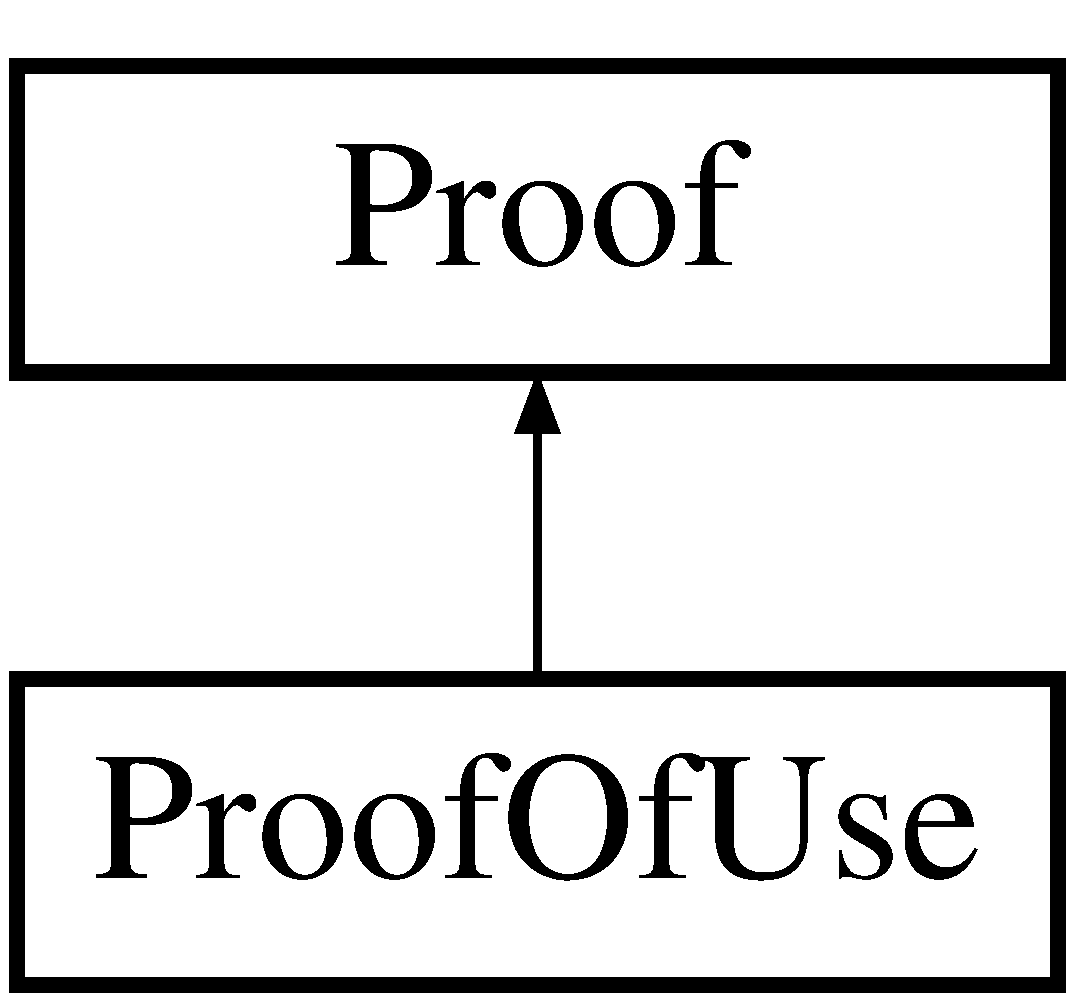
\includegraphics[height=2.000000cm]{classProofOfUse}
\end{center}
\end{figure}
\subsection*{Public Member Functions}
\begin{DoxyCompactItemize}
\item 
void \mbox{\hyperlink{classProofOfUse_aefccdad0aa3344b6331acecc05299cc0}{run}} (\mbox{\hyperlink{classBlock}{Block}} $\ast$block, std\+::string key) const override
\item 
bool \mbox{\hyperlink{classProofOfUse_a315614eb2b05b40367bdc11e60b7b8be}{accept}} (\mbox{\hyperlink{classBlock}{Block}} $\ast$block, \mbox{\hyperlink{classMessage}{Message}} $\ast$message) const override
\end{DoxyCompactItemize}
\subsection*{Static Public Member Functions}
\begin{DoxyCompactItemize}
\item 
static void \mbox{\hyperlink{classProof_a71874539fdbcc93c15594b889c95225b}{add\+\_\+proof}} (int id, std\+::function$<$ \mbox{\hyperlink{classProof}{Proof}} $\ast$()$>$ proof)
\item 
static \mbox{\hyperlink{classProof}{Proof}} $\ast$ \mbox{\hyperlink{classProof_a267f0f4587babb59884b5f280e2d54c8}{generate}} (int type)
\end{DoxyCompactItemize}
\subsection*{Static Public Attributes}
\begin{DoxyCompactItemize}
\item 
\mbox{\Hypertarget{classProof_a457d231986439ee6bcc945daacfc28fc}\label{classProof_a457d231986439ee6bcc945daacfc28fc}} 
static const int {\bfseries W\+O\+RK} = 0
\item 
\mbox{\Hypertarget{classProof_acf157976c3c86ef2fd0e838b8c4ac992}\label{classProof_acf157976c3c86ef2fd0e838b8c4ac992}} 
static const int {\bfseries S\+T\+A\+KE} = 1
\item 
\mbox{\Hypertarget{classProof_ae5c2a86640bf558ff5625157e23b3eec}\label{classProof_ae5c2a86640bf558ff5625157e23b3eec}} 
static const int {\bfseries H\+O\+LD} = 2
\item 
\mbox{\Hypertarget{classProof_a4e71a5e5928900794353acdd169ca652}\label{classProof_a4e71a5e5928900794353acdd169ca652}} 
static const int {\bfseries I\+M\+P\+O\+R\+T\+A\+N\+CE} = 3
\item 
\mbox{\Hypertarget{classProof_a1a08ffc465f4fcfde396d4c4feb22eb0}\label{classProof_a1a08ffc465f4fcfde396d4c4feb22eb0}} 
static const int {\bfseries M\+I\+N\+I\+M\+U\+M\+\_\+\+A\+G\+E\+D\+\_\+\+S\+T\+A\+KE} = 4
\item 
\mbox{\Hypertarget{classProof_a1aa2cb91c5be4ca021714ff6fc01da4a}\label{classProof_a1aa2cb91c5be4ca021714ff6fc01da4a}} 
static const int {\bfseries S\+T\+A\+K\+E\+\_\+\+T\+I\+ME} = 5
\item 
\mbox{\Hypertarget{classProof_a3f6898fa1d652d32182c3c387c8e979c}\label{classProof_a3f6898fa1d652d32182c3c387c8e979c}} 
static const int {\bfseries U\+SE} = 6
\end{DoxyCompactItemize}


\subsection{Detailed Description}
A basic proof of use \begin{DoxySeeAlso}{See also}
\mbox{\hyperlink{classProof}{Proof}} 

Proof\+::\+U\+SE
\end{DoxySeeAlso}
\begin{DoxyAuthor}{Author}
Mathieu Lochet 
\end{DoxyAuthor}
\begin{DoxyVersion}{Version}
1 
\end{DoxyVersion}


\subsection{Member Function Documentation}
\mbox{\Hypertarget{classProofOfUse_a315614eb2b05b40367bdc11e60b7b8be}\label{classProofOfUse_a315614eb2b05b40367bdc11e60b7b8be}} 
\index{Proof\+Of\+Use@{Proof\+Of\+Use}!accept@{accept}}
\index{accept@{accept}!Proof\+Of\+Use@{Proof\+Of\+Use}}
\subsubsection{\texorpdfstring{accept()}{accept()}}
{\footnotesize\ttfamily bool Proof\+Of\+Use\+::accept (\begin{DoxyParamCaption}\item[{\mbox{\hyperlink{classBlock}{Block}} $\ast$}]{block,  }\item[{\mbox{\hyperlink{classMessage}{Message}} $\ast$}]{ }\end{DoxyParamCaption}) const\hspace{0.3cm}{\ttfamily [override]}, {\ttfamily [virtual]}}

Get a proof result and check if the result is correct Needs to be implemented


\begin{DoxyParams}{Parameters}
{\em block} & The block to check the proof \\
\hline
{\em The} & received message \\
\hline
\end{DoxyParams}


Implements \mbox{\hyperlink{classProof_a358b3883eb33b8ecc93f74cb6313679a}{Proof}}.

\mbox{\Hypertarget{classProof_a71874539fdbcc93c15594b889c95225b}\label{classProof_a71874539fdbcc93c15594b889c95225b}} 
\index{Proof\+Of\+Use@{Proof\+Of\+Use}!add\+\_\+proof@{add\+\_\+proof}}
\index{add\+\_\+proof@{add\+\_\+proof}!Proof\+Of\+Use@{Proof\+Of\+Use}}
\subsubsection{\texorpdfstring{add\+\_\+proof()}{add\_proof()}}
{\footnotesize\ttfamily void Proof\+::add\+\_\+proof (\begin{DoxyParamCaption}\item[{int}]{id,  }\item[{std\+::function$<$ \mbox{\hyperlink{classProof}{Proof}} $\ast$()$>$}]{proof }\end{DoxyParamCaption})\hspace{0.3cm}{\ttfamily [static]}, {\ttfamily [inherited]}}

Allows the user to add its own proof into the system He the proof id is required


\begin{DoxyParams}{Parameters}
{\em id} & The proof id \\
\hline
{\em proof} & The lambda expression that creates a proof \\
\hline
\end{DoxyParams}
\mbox{\Hypertarget{classProof_a267f0f4587babb59884b5f280e2d54c8}\label{classProof_a267f0f4587babb59884b5f280e2d54c8}} 
\index{Proof\+Of\+Use@{Proof\+Of\+Use}!generate@{generate}}
\index{generate@{generate}!Proof\+Of\+Use@{Proof\+Of\+Use}}
\subsubsection{\texorpdfstring{generate()}{generate()}}
{\footnotesize\ttfamily \mbox{\hyperlink{classProof}{Proof}} $\ast$ Proof\+::generate (\begin{DoxyParamCaption}\item[{int}]{type }\end{DoxyParamCaption})\hspace{0.3cm}{\ttfamily [static]}, {\ttfamily [inherited]}}

Generates a proof for a given id


\begin{DoxyParams}{Parameters}
{\em id} & The proof id \\
\hline
\end{DoxyParams}
\begin{DoxyReturn}{Returns}
The created proof object 
\end{DoxyReturn}
\mbox{\Hypertarget{classProofOfUse_aefccdad0aa3344b6331acecc05299cc0}\label{classProofOfUse_aefccdad0aa3344b6331acecc05299cc0}} 
\index{Proof\+Of\+Use@{Proof\+Of\+Use}!run@{run}}
\index{run@{run}!Proof\+Of\+Use@{Proof\+Of\+Use}}
\subsubsection{\texorpdfstring{run()}{run()}}
{\footnotesize\ttfamily void Proof\+Of\+Use\+::run (\begin{DoxyParamCaption}\item[{\mbox{\hyperlink{classBlock}{Block}} $\ast$}]{block,  }\item[{std\+::string}]{key }\end{DoxyParamCaption}) const\hspace{0.3cm}{\ttfamily [override]}, {\ttfamily [virtual]}}

Run a proof on a block to validate it Needs to be implemented


\begin{DoxyParams}{Parameters}
{\em block} & The block to run the proof on \\
\hline
{\em The} & user\textquotesingle{}s key to use in the process \\
\hline
\end{DoxyParams}


Implements \mbox{\hyperlink{classProof_a6ab9f6c3f603447e3a9c7c932b5deac4}{Proof}}.



The documentation for this class was generated from the following files\+:\begin{DoxyCompactItemize}
\item 
block\+\_\+chain/chain/block/proof/Proof\+Of\+Use.\+h\item 
block\+\_\+chain/chain/block/proof/Proof\+Of\+Use.\+cpp\end{DoxyCompactItemize}

\hypertarget{classProofOfWork}{}\section{Proof\+Of\+Work Class Reference}
\label{classProofOfWork}\index{Proof\+Of\+Work@{Proof\+Of\+Work}}


{\ttfamily \#include $<$Proof\+Of\+Work.\+h$>$}

Inheritance diagram for Proof\+Of\+Work\+:\begin{figure}[H]
\begin{center}
\leavevmode
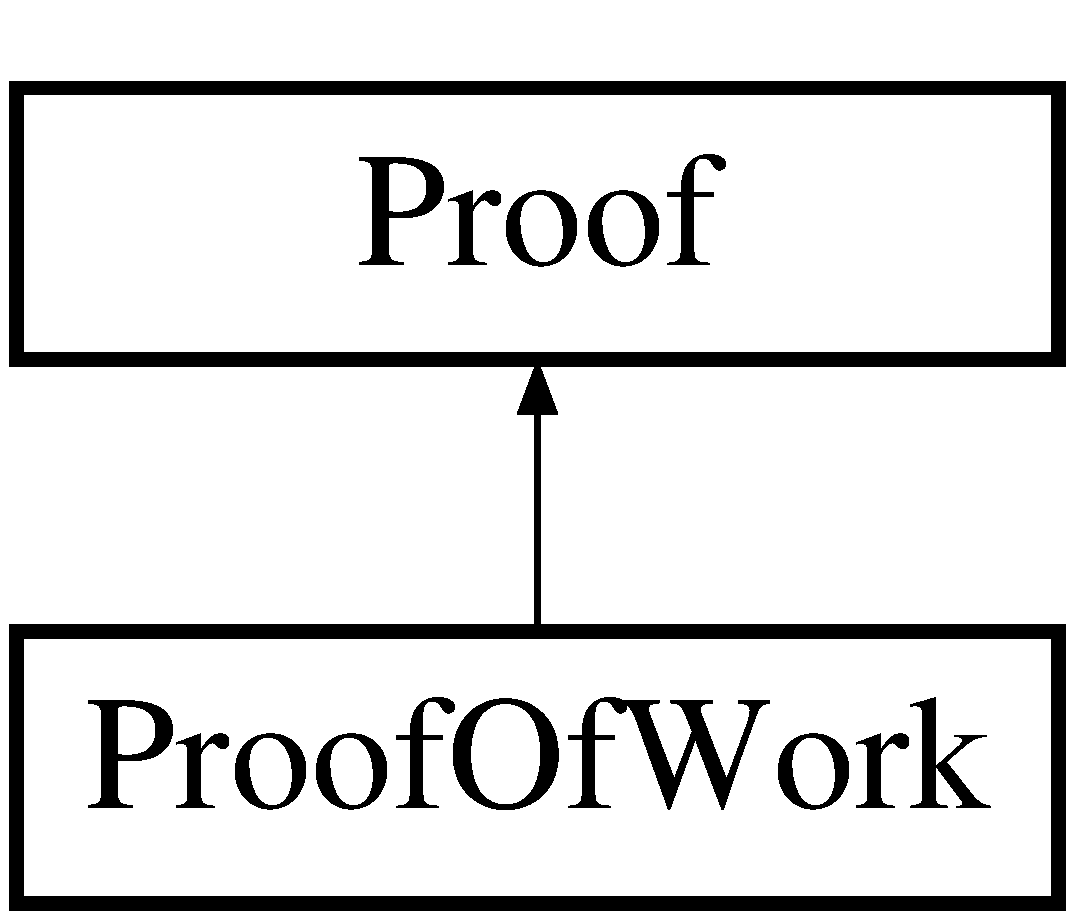
\includegraphics[height=2.000000cm]{classProofOfWork}
\end{center}
\end{figure}
\subsection*{Public Member Functions}
\begin{DoxyCompactItemize}
\item 
void \mbox{\hyperlink{classProofOfWork_a80cbd012ee3f9e92a8497efac84bf689}{run}} (\mbox{\hyperlink{classBlock}{Block}} $\ast$block, std\+::string key) override
\item 
bool \mbox{\hyperlink{classProofOfWork_abe3dba92dad383eec07f70acccaa802d}{accept}} (\mbox{\hyperlink{classBlock}{Block}} $\ast$block, \mbox{\hyperlink{classMessage}{Message}} $\ast$) override
\end{DoxyCompactItemize}
\subsection*{Static Public Member Functions}
\begin{DoxyCompactItemize}
\item 
static void \mbox{\hyperlink{classProof_a71874539fdbcc93c15594b889c95225b}{add\+\_\+proof}} (int id, std\+::function$<$ \mbox{\hyperlink{classProof}{Proof}} $\ast$()$>$ proof)
\item 
static \mbox{\hyperlink{classProof}{Proof}} $\ast$ \mbox{\hyperlink{classProof_a267f0f4587babb59884b5f280e2d54c8}{generate}} (int type)
\end{DoxyCompactItemize}
\subsection*{Static Public Attributes}
\begin{DoxyCompactItemize}
\item 
\mbox{\Hypertarget{classProof_a457d231986439ee6bcc945daacfc28fc}\label{classProof_a457d231986439ee6bcc945daacfc28fc}} 
static const int {\bfseries W\+O\+RK} = 0
\item 
\mbox{\Hypertarget{classProof_acf157976c3c86ef2fd0e838b8c4ac992}\label{classProof_acf157976c3c86ef2fd0e838b8c4ac992}} 
static const int {\bfseries S\+T\+A\+KE} = 1
\item 
\mbox{\Hypertarget{classProof_ae5c2a86640bf558ff5625157e23b3eec}\label{classProof_ae5c2a86640bf558ff5625157e23b3eec}} 
static const int {\bfseries H\+O\+LD} = 2
\item 
\mbox{\Hypertarget{classProof_a4e71a5e5928900794353acdd169ca652}\label{classProof_a4e71a5e5928900794353acdd169ca652}} 
static const int {\bfseries I\+M\+P\+O\+R\+T\+A\+N\+CE} = 3
\item 
\mbox{\Hypertarget{classProof_a1a08ffc465f4fcfde396d4c4feb22eb0}\label{classProof_a1a08ffc465f4fcfde396d4c4feb22eb0}} 
static const int {\bfseries M\+I\+N\+I\+M\+U\+M\+\_\+\+A\+G\+E\+D\+\_\+\+S\+T\+A\+KE} = 4
\item 
\mbox{\Hypertarget{classProof_a1aa2cb91c5be4ca021714ff6fc01da4a}\label{classProof_a1aa2cb91c5be4ca021714ff6fc01da4a}} 
static const int {\bfseries S\+T\+A\+K\+E\+\_\+\+T\+I\+ME} = 5
\item 
\mbox{\Hypertarget{classProof_a3f6898fa1d652d32182c3c387c8e979c}\label{classProof_a3f6898fa1d652d32182c3c387c8e979c}} 
static const int {\bfseries U\+SE} = 6
\end{DoxyCompactItemize}


\subsection{Detailed Description}
A basic proof of work \begin{DoxySeeAlso}{See also}
\mbox{\hyperlink{classProof}{Proof}} 

Proof\+::\+W\+O\+RK
\end{DoxySeeAlso}
\begin{DoxyAuthor}{Author}
Mathieu Lochet 
\end{DoxyAuthor}
\begin{DoxyVersion}{Version}
1 
\end{DoxyVersion}


\subsection{Member Function Documentation}
\mbox{\Hypertarget{classProofOfWork_abe3dba92dad383eec07f70acccaa802d}\label{classProofOfWork_abe3dba92dad383eec07f70acccaa802d}} 
\index{Proof\+Of\+Work@{Proof\+Of\+Work}!accept@{accept}}
\index{accept@{accept}!Proof\+Of\+Work@{Proof\+Of\+Work}}
\subsubsection{\texorpdfstring{accept()}{accept()}}
{\footnotesize\ttfamily bool Proof\+Of\+Work\+::accept (\begin{DoxyParamCaption}\item[{\mbox{\hyperlink{classBlock}{Block}} $\ast$}]{block,  }\item[{\mbox{\hyperlink{classMessage}{Message}} $\ast$}]{ }\end{DoxyParamCaption})\hspace{0.3cm}{\ttfamily [override]}, {\ttfamily [virtual]}}

Get a proof result and check if the result is correct Needs to be implemented


\begin{DoxyParams}{Parameters}
{\em block} & The block to check the proof \\
\hline
{\em The} & received message \\
\hline
\end{DoxyParams}


Implements \mbox{\hyperlink{classProof_ad52fee058ea617a186133cb6a008fe6e}{Proof}}.

\mbox{\Hypertarget{classProof_a71874539fdbcc93c15594b889c95225b}\label{classProof_a71874539fdbcc93c15594b889c95225b}} 
\index{Proof\+Of\+Work@{Proof\+Of\+Work}!add\+\_\+proof@{add\+\_\+proof}}
\index{add\+\_\+proof@{add\+\_\+proof}!Proof\+Of\+Work@{Proof\+Of\+Work}}
\subsubsection{\texorpdfstring{add\+\_\+proof()}{add\_proof()}}
{\footnotesize\ttfamily void Proof\+::add\+\_\+proof (\begin{DoxyParamCaption}\item[{int}]{id,  }\item[{std\+::function$<$ \mbox{\hyperlink{classProof}{Proof}} $\ast$()$>$}]{proof }\end{DoxyParamCaption})\hspace{0.3cm}{\ttfamily [static]}, {\ttfamily [inherited]}}

Allows the user to add its own proof into the system He the proof id is required


\begin{DoxyParams}{Parameters}
{\em id} & The proof id \\
\hline
{\em proof} & The lambda expression that creates a proof \\
\hline
\end{DoxyParams}
\mbox{\Hypertarget{classProof_a267f0f4587babb59884b5f280e2d54c8}\label{classProof_a267f0f4587babb59884b5f280e2d54c8}} 
\index{Proof\+Of\+Work@{Proof\+Of\+Work}!generate@{generate}}
\index{generate@{generate}!Proof\+Of\+Work@{Proof\+Of\+Work}}
\subsubsection{\texorpdfstring{generate()}{generate()}}
{\footnotesize\ttfamily \mbox{\hyperlink{classProof}{Proof}} $\ast$ Proof\+::generate (\begin{DoxyParamCaption}\item[{int}]{type }\end{DoxyParamCaption})\hspace{0.3cm}{\ttfamily [static]}, {\ttfamily [inherited]}}

Generates a proof for a given id


\begin{DoxyParams}{Parameters}
{\em id} & The proof id \\
\hline
\end{DoxyParams}
\begin{DoxyReturn}{Returns}
The created proof object 
\end{DoxyReturn}
\mbox{\Hypertarget{classProofOfWork_a80cbd012ee3f9e92a8497efac84bf689}\label{classProofOfWork_a80cbd012ee3f9e92a8497efac84bf689}} 
\index{Proof\+Of\+Work@{Proof\+Of\+Work}!run@{run}}
\index{run@{run}!Proof\+Of\+Work@{Proof\+Of\+Work}}
\subsubsection{\texorpdfstring{run()}{run()}}
{\footnotesize\ttfamily void Proof\+Of\+Work\+::run (\begin{DoxyParamCaption}\item[{\mbox{\hyperlink{classBlock}{Block}} $\ast$}]{block,  }\item[{std\+::string}]{key }\end{DoxyParamCaption})\hspace{0.3cm}{\ttfamily [override]}, {\ttfamily [virtual]}}

Run a proof on a block to validate it Needs to be implemented


\begin{DoxyParams}{Parameters}
{\em block} & The block to run the proof on \\
\hline
{\em The} & user\textquotesingle{}s key to use in the process \\
\hline
\end{DoxyParams}


Implements \mbox{\hyperlink{classProof_a8a43fcb7c997da54d627e0f257adb86f}{Proof}}.



The documentation for this class was generated from the following files\+:\begin{DoxyCompactItemize}
\item 
block\+\_\+chain/chain/block/proof/Proof\+Of\+Work.\+h\item 
block\+\_\+chain/chain/block/proof/Proof\+Of\+Work.\+cpp\end{DoxyCompactItemize}

\hypertarget{classProofOfWorkMetadata}{}\section{Proof\+Of\+Work\+Metadata Class Reference}
\label{classProofOfWorkMetadata}\index{Proof\+Of\+Work\+Metadata@{Proof\+Of\+Work\+Metadata}}


{\ttfamily \#include $<$Proof\+Of\+Work\+Metadata.\+h$>$}

Inheritance diagram for Proof\+Of\+Work\+Metadata\+:\begin{figure}[H]
\begin{center}
\leavevmode
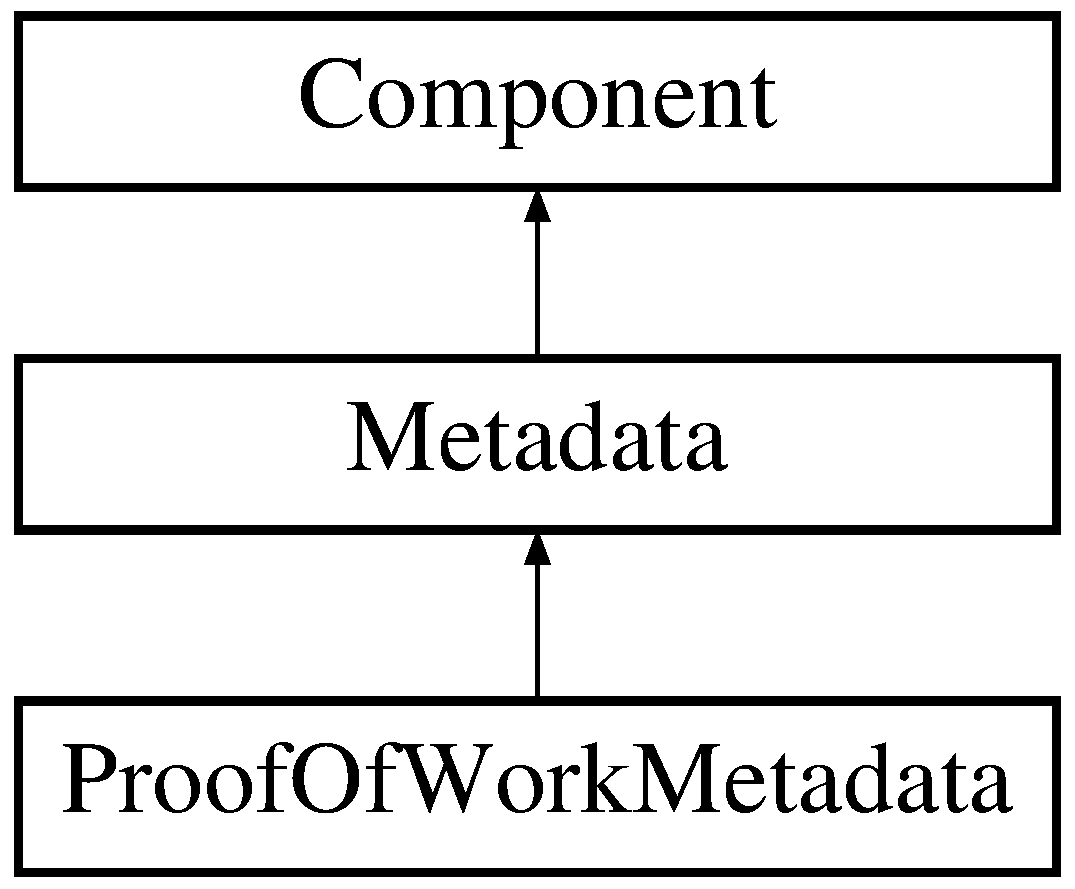
\includegraphics[height=3.000000cm]{classProofOfWorkMetadata}
\end{center}
\end{figure}
\subsection*{Public Member Functions}
\begin{DoxyCompactItemize}
\item 
\mbox{\hyperlink{classProofOfWorkMetadata_a8fe975e4a12a0782becb25d1d5683a21}{Proof\+Of\+Work\+Metadata}} (long long int i1, long long int i2, std\+::string str)
\item 
bool \mbox{\hyperlink{classProofOfWorkMetadata_ae490506a28967c7180163fc156dd5d51}{operator==}} (\mbox{\hyperlink{classMetadata}{Metadata}} \&m) const override
\item 
\mbox{\hyperlink{classElement}{Element}} $\ast$ \mbox{\hyperlink{classProofOfWorkMetadata_a2aab4c26afb3a85a712cc065028274d9}{to\+Element}} () const override
\item 
\mbox{\hyperlink{classHash}{Hash}} $\ast$ \mbox{\hyperlink{classProofOfWorkMetadata_af29f8f40d4b438eaa9434b51c1aff7c6}{hash}} () override
\item 
void \mbox{\hyperlink{classProofOfWorkMetadata_add9667954ffeaee75f3329c6c832e8b7}{update\+\_\+database}} (\mbox{\hyperlink{classDatabase}{Database}} $\ast$p\+Database) override
\item 
void \mbox{\hyperlink{classComponent_a28212595f8ee85fe009bd233bc99b2fc}{\+\_\+\+\_\+init\+\_\+\+\_\+}} (\mbox{\hyperlink{classElementObject}{Element\+Object}} $\ast$element, const \mbox{\hyperlink{classSerializer}{Serializer}} $\ast$s, const char $\ast$encoding)
\end{DoxyCompactItemize}
\subsection*{Protected Member Functions}
\begin{DoxyCompactItemize}
\item 
void \mbox{\hyperlink{classProofOfWorkMetadata_afac533eee3123bce72615ab90f7c9669}{from\+Element}} (\mbox{\hyperlink{classElementObject}{Element\+Object}} $\ast$e, const \mbox{\hyperlink{classSerializer}{Serializer}} $\ast$s, const char $\ast$encoding) override
\end{DoxyCompactItemize}
\subsection*{Friends}
\begin{DoxyCompactItemize}
\item 
\mbox{\Hypertarget{classProofOfWorkMetadata_a5493b64dfe8bc707452f326c6ec29f14}\label{classProofOfWorkMetadata_a5493b64dfe8bc707452f326c6ec29f14}} 
class {\bfseries Proof\+Of\+Work}
\end{DoxyCompactItemize}


\subsection{Detailed Description}
An metadata class for the proof of work. \begin{DoxySeeAlso}{See also}
\mbox{\hyperlink{classBlock}{Block}} 

\mbox{\hyperlink{classProofOfWork}{Proof\+Of\+Work}}
\end{DoxySeeAlso}
\begin{DoxyAuthor}{Author}
Mathieu Lochet 
\end{DoxyAuthor}
\begin{DoxyVersion}{Version}
1 
\end{DoxyVersion}


\subsection{Constructor \& Destructor Documentation}
\mbox{\Hypertarget{classProofOfWorkMetadata_a8fe975e4a12a0782becb25d1d5683a21}\label{classProofOfWorkMetadata_a8fe975e4a12a0782becb25d1d5683a21}} 
\index{Proof\+Of\+Work\+Metadata@{Proof\+Of\+Work\+Metadata}!Proof\+Of\+Work\+Metadata@{Proof\+Of\+Work\+Metadata}}
\index{Proof\+Of\+Work\+Metadata@{Proof\+Of\+Work\+Metadata}!Proof\+Of\+Work\+Metadata@{Proof\+Of\+Work\+Metadata}}
\subsubsection{\texorpdfstring{Proof\+Of\+Work\+Metadata()}{ProofOfWorkMetadata()}}
{\footnotesize\ttfamily Proof\+Of\+Work\+Metadata\+::\+Proof\+Of\+Work\+Metadata (\begin{DoxyParamCaption}\item[{long long int}]{i1,  }\item[{long long int}]{i2,  }\item[{std\+::string}]{str }\end{DoxyParamCaption})}

Generated the metadata with the given parameters


\begin{DoxyParams}{Parameters}
{\em i1} & The first hash parameter \\
\hline
{\em i2} & The second hash parameter \\
\hline
{\em str} & The winner\textquotesingle{}s public key \\
\hline
\end{DoxyParams}


\subsection{Member Function Documentation}
\mbox{\Hypertarget{classComponent_a28212595f8ee85fe009bd233bc99b2fc}\label{classComponent_a28212595f8ee85fe009bd233bc99b2fc}} 
\index{Proof\+Of\+Work\+Metadata@{Proof\+Of\+Work\+Metadata}!\+\_\+\+\_\+init\+\_\+\+\_\+@{\+\_\+\+\_\+init\+\_\+\+\_\+}}
\index{\+\_\+\+\_\+init\+\_\+\+\_\+@{\+\_\+\+\_\+init\+\_\+\+\_\+}!Proof\+Of\+Work\+Metadata@{Proof\+Of\+Work\+Metadata}}
\subsubsection{\texorpdfstring{\+\_\+\+\_\+init\+\_\+\+\_\+()}{\_\_init\_\_()}}
{\footnotesize\ttfamily void Component\+::\+\_\+\+\_\+init\+\_\+\+\_\+ (\begin{DoxyParamCaption}\item[{\mbox{\hyperlink{classElementObject}{Element\+Object}} $\ast$}]{element,  }\item[{const \mbox{\hyperlink{classSerializer}{Serializer}} $\ast$}]{s,  }\item[{const char $\ast$}]{encoding }\end{DoxyParamCaption})\hspace{0.3cm}{\ttfamily [inline]}, {\ttfamily [inherited]}}

The function called by the serializer to initialize the object if it is empty \begin{DoxySeeAlso}{See also}
\mbox{\hyperlink{classElementObject}{Element\+Object}} 

\mbox{\hyperlink{classSerializer}{Serializer}}
\end{DoxySeeAlso}

\begin{DoxyParams}{Parameters}
{\em element} & The \mbox{\hyperlink{classElement}{Element}} representation of the object \\
\hline
{\em s} & The serializer (Can be used if serialization of some elements is needed) \\
\hline
{\em encoding} & The encoding that has been used to create the \mbox{\hyperlink{classElement}{Element}} representation of the object (Can be used if serialization of some elements is needed) \\
\hline
\end{DoxyParams}
\mbox{\Hypertarget{classProofOfWorkMetadata_afac533eee3123bce72615ab90f7c9669}\label{classProofOfWorkMetadata_afac533eee3123bce72615ab90f7c9669}} 
\index{Proof\+Of\+Work\+Metadata@{Proof\+Of\+Work\+Metadata}!from\+Element@{from\+Element}}
\index{from\+Element@{from\+Element}!Proof\+Of\+Work\+Metadata@{Proof\+Of\+Work\+Metadata}}
\subsubsection{\texorpdfstring{from\+Element()}{fromElement()}}
{\footnotesize\ttfamily void Proof\+Of\+Work\+Metadata\+::from\+Element (\begin{DoxyParamCaption}\item[{\mbox{\hyperlink{classElementObject}{Element\+Object}} $\ast$}]{,  }\item[{const \mbox{\hyperlink{classSerializer}{Serializer}} $\ast$}]{,  }\item[{const char $\ast$}]{encoding }\end{DoxyParamCaption})\hspace{0.3cm}{\ttfamily [override]}, {\ttfamily [protected]}, {\ttfamily [virtual]}}

The function used to build the object from its element representation. the object if it is empty \begin{DoxySeeAlso}{See also}
\mbox{\hyperlink{classElementObject}{Element\+Object}} 

\mbox{\hyperlink{classSerializer}{Serializer}}
\end{DoxySeeAlso}

\begin{DoxyParams}{Parameters}
{\em element} & The \mbox{\hyperlink{classElement}{Element}} representation of the object \\
\hline
{\em s} & The serializer (Can be used if serialization of some elements is needed) \\
\hline
{\em encoding} & The encoding that has been used to create the \mbox{\hyperlink{classElement}{Element}} representation of the object (Can be used if serialization of some elements is needed) \\
\hline
\end{DoxyParams}


Implements \mbox{\hyperlink{classComponent_a2ded18881226d0077dc393e0e9304bb1}{Component}}.

\mbox{\Hypertarget{classProofOfWorkMetadata_af29f8f40d4b438eaa9434b51c1aff7c6}\label{classProofOfWorkMetadata_af29f8f40d4b438eaa9434b51c1aff7c6}} 
\index{Proof\+Of\+Work\+Metadata@{Proof\+Of\+Work\+Metadata}!hash@{hash}}
\index{hash@{hash}!Proof\+Of\+Work\+Metadata@{Proof\+Of\+Work\+Metadata}}
\subsubsection{\texorpdfstring{hash()}{hash()}}
{\footnotesize\ttfamily \mbox{\hyperlink{classHash}{Hash}} $\ast$ Proof\+Of\+Work\+Metadata\+::hash (\begin{DoxyParamCaption}{ }\end{DoxyParamCaption})\hspace{0.3cm}{\ttfamily [override]}, {\ttfamily [virtual]}}

Get the hash ofthe user who validated the block

\begin{DoxyReturn}{Returns}
The hash ofthe user who validated the block 
\end{DoxyReturn}


Implements \mbox{\hyperlink{classMetadata_a893b85a8fe38060c72bdda20818a7334}{Metadata}}.

\mbox{\Hypertarget{classProofOfWorkMetadata_ae490506a28967c7180163fc156dd5d51}\label{classProofOfWorkMetadata_ae490506a28967c7180163fc156dd5d51}} 
\index{Proof\+Of\+Work\+Metadata@{Proof\+Of\+Work\+Metadata}!operator==@{operator==}}
\index{operator==@{operator==}!Proof\+Of\+Work\+Metadata@{Proof\+Of\+Work\+Metadata}}
\subsubsection{\texorpdfstring{operator==()}{operator==()}}
{\footnotesize\ttfamily bool Proof\+Of\+Work\+Metadata\+::operator== (\begin{DoxyParamCaption}\item[{\mbox{\hyperlink{classMetadata}{Metadata}} \&}]{m }\end{DoxyParamCaption}) const\hspace{0.3cm}{\ttfamily [inline]}, {\ttfamily [override]}, {\ttfamily [virtual]}}

Overriding the == operator


\begin{DoxyParams}{Parameters}
{\em m} & A metadata to be compared \\
\hline
\end{DoxyParams}
\begin{DoxyReturn}{Returns}
true if the conditions are satisfied, false otherwise 
\end{DoxyReturn}


Reimplemented from \mbox{\hyperlink{classMetadata_a2721356452a5d366d58275dd1fc1209c}{Metadata}}.

\mbox{\Hypertarget{classProofOfWorkMetadata_a2aab4c26afb3a85a712cc065028274d9}\label{classProofOfWorkMetadata_a2aab4c26afb3a85a712cc065028274d9}} 
\index{Proof\+Of\+Work\+Metadata@{Proof\+Of\+Work\+Metadata}!to\+Element@{to\+Element}}
\index{to\+Element@{to\+Element}!Proof\+Of\+Work\+Metadata@{Proof\+Of\+Work\+Metadata}}
\subsubsection{\texorpdfstring{to\+Element()}{toElement()}}
{\footnotesize\ttfamily \mbox{\hyperlink{classElement}{Element}} $\ast$ Proof\+Of\+Work\+Metadata\+::to\+Element (\begin{DoxyParamCaption}{ }\end{DoxyParamCaption}) const\hspace{0.3cm}{\ttfamily [override]}, {\ttfamily [virtual]}}

The method used by the serializer to transform an object into an \mbox{\hyperlink{classElement}{Element}} representation. \begin{DoxySeeAlso}{See also}
\mbox{\hyperlink{classElement}{Element}}
\end{DoxySeeAlso}
\begin{DoxyReturn}{Returns}
The \mbox{\hyperlink{classElement}{Element}} representation of the object 
\end{DoxyReturn}


Implements \mbox{\hyperlink{classComponent_a3e63d8c993e417a4af3f56d65ebfc7ea}{Component}}.

\mbox{\Hypertarget{classProofOfWorkMetadata_add9667954ffeaee75f3329c6c832e8b7}\label{classProofOfWorkMetadata_add9667954ffeaee75f3329c6c832e8b7}} 
\index{Proof\+Of\+Work\+Metadata@{Proof\+Of\+Work\+Metadata}!update\+\_\+database@{update\+\_\+database}}
\index{update\+\_\+database@{update\+\_\+database}!Proof\+Of\+Work\+Metadata@{Proof\+Of\+Work\+Metadata}}
\subsubsection{\texorpdfstring{update\+\_\+database()}{update\_database()}}
{\footnotesize\ttfamily void Proof\+Of\+Work\+Metadata\+::update\+\_\+database (\begin{DoxyParamCaption}\item[{\mbox{\hyperlink{classDatabase}{Database}} $\ast$}]{d }\end{DoxyParamCaption})\hspace{0.3cm}{\ttfamily [override]}, {\ttfamily [virtual]}}

Update the database with the reward transaction when the block is validated


\begin{DoxyParams}{Parameters}
{\em d} & The database to update \\
\hline
\end{DoxyParams}


Implements \mbox{\hyperlink{classMetadata_a501ab1977aac6a75f92309284e17de30}{Metadata}}.



The documentation for this class was generated from the following files\+:\begin{DoxyCompactItemize}
\item 
block\+\_\+chain/chain/block/proof/metadatas/Proof\+Of\+Work\+Metadata.\+h\item 
block\+\_\+chain/chain/block/proof/metadatas/Proof\+Of\+Work\+Metadata.\+cpp\end{DoxyCompactItemize}

\hypertarget{classReward}{}\section{Reward Class Reference}
\label{classReward}\index{Reward@{Reward}}


{\ttfamily \#include $<$Reward.\+h$>$}

Inheritance diagram for Reward\+:\begin{figure}[H]
\begin{center}
\leavevmode
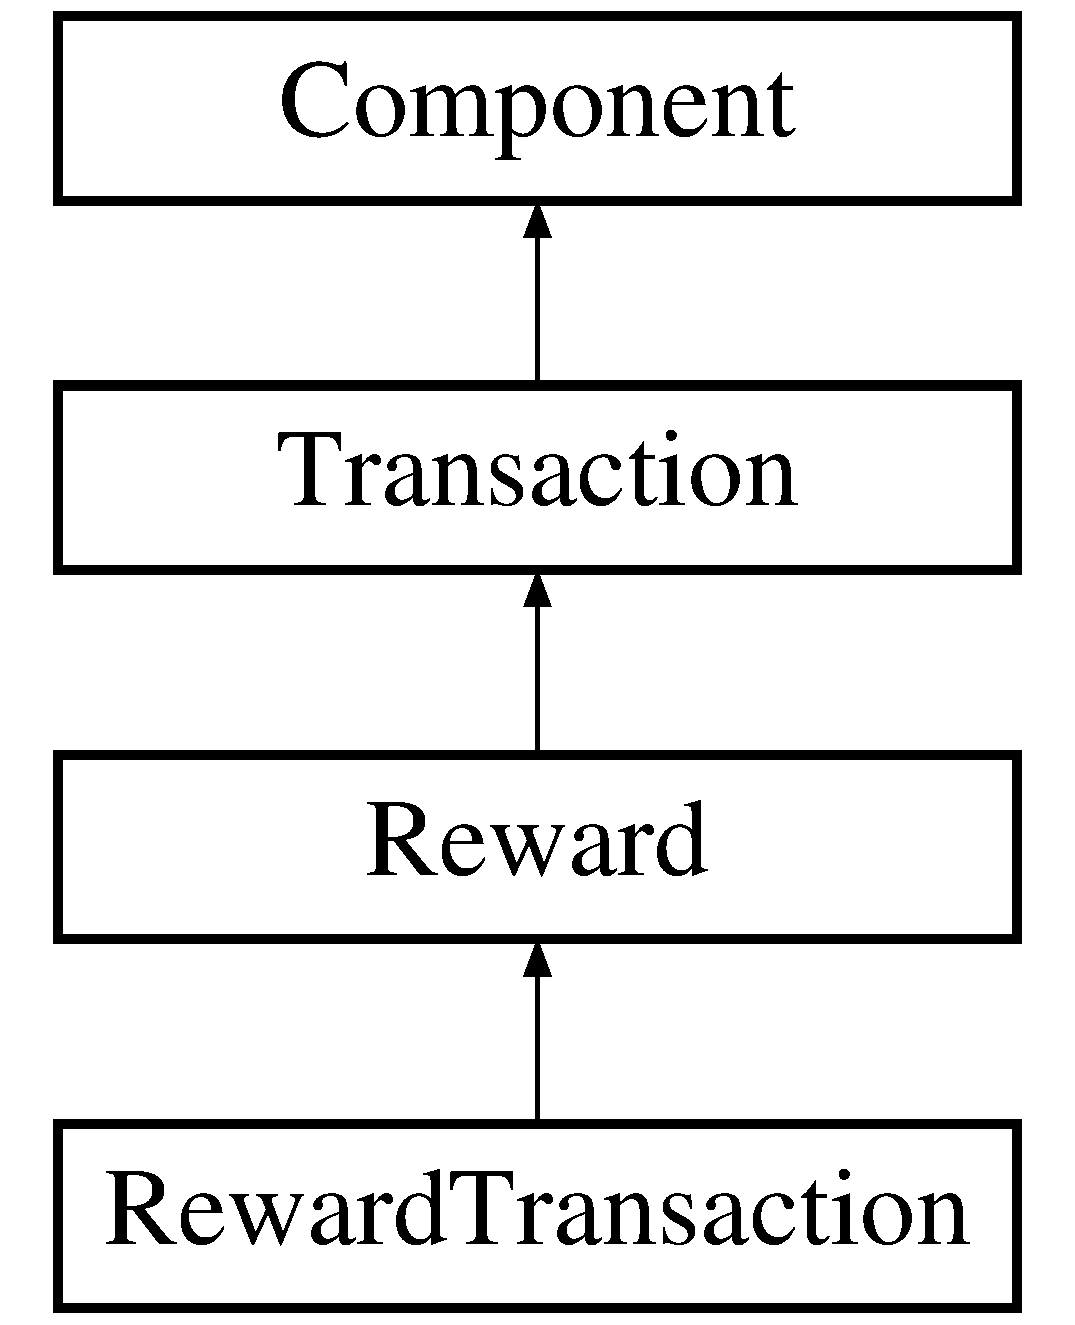
\includegraphics[height=4.000000cm]{classReward}
\end{center}
\end{figure}
\subsection*{Public Member Functions}
\begin{DoxyCompactItemize}
\item 
\mbox{\hyperlink{classElement}{Element}} $\ast$ \mbox{\hyperlink{classReward_a0ecd536148463880f9980fe415b6eb1d}{to\+Element}} () const final
\item 
bool \mbox{\hyperlink{classReward_ab2cd65f16c670e3e9d8cfe84a6dc56cb}{operator==}} (\mbox{\hyperlink{classTransaction}{Transaction}} $\ast$t) const final
\item 
\mbox{\Hypertarget{classReward_a0d65cd39eb260091d1f2cf19e2e71de7}\label{classReward_a0d65cd39eb260091d1f2cf19e2e71de7}} 
std\+::string {\bfseries to\+\_\+string} () const
\item 
void \mbox{\hyperlink{classReward_a494c9d6e0a220729f675fd6131cfb9af}{apply\+\_\+reverse}} (\mbox{\hyperlink{classRow}{Row}} $\ast$row) final
\item 
bool \mbox{\hyperlink{classReward_a9c9a3219ba6b8b068f7f1cccc779b1b5}{validate}} (\mbox{\hyperlink{classRow}{Row}} $\ast$row) const final
\item 
int \mbox{\hyperlink{classReward_a1d3d05263d54771a314927d09585968c}{get\+\_\+type}} () const final
\item 
std\+::string \mbox{\hyperlink{classReward_a95e98fc9dbbc9da47cee243adc1932d2}{description}} () const final
\item 
void \mbox{\hyperlink{classReward_a30a40e2eefd0aea969fab46d1e22d145}{fill\+\_\+data}} () final
\item 
std\+::vector$<$ std\+::string $>$ \mbox{\hyperlink{classReward_aae55ec2aa2aa31cc365c80cb42be9ab5}{apply}} (\mbox{\hyperlink{classRow}{Row}} $\ast$row) override
\item 
\mbox{\hyperlink{classHash}{Hash}} $\ast$ \mbox{\hyperlink{classTransaction_a1f0df166c34d6a38a991544cf98c0356}{\+\_\+\+\_\+hash\+\_\+\+\_\+}} (const \mbox{\hyperlink{classSerializer}{Serializer}} $\ast$serializer, const char $\ast$encoding) const
\item 
virtual \mbox{\hyperlink{classRow}{Row}} $\ast$ \mbox{\hyperlink{classTransaction_aa80b621537fe480dcb4444bba703abe5}{create\+Row}} () const =0
\item 
virtual \mbox{\hyperlink{classTransaction}{Transaction}} $\ast$ \mbox{\hyperlink{classTransaction_ad6ee9c5e4067b2f5c950c6aad131b3e4}{clone}} ()=0
\item 
void \mbox{\hyperlink{classComponent_a28212595f8ee85fe009bd233bc99b2fc}{\+\_\+\+\_\+init\+\_\+\+\_\+}} (\mbox{\hyperlink{classElementObject}{Element\+Object}} $\ast$element, const \mbox{\hyperlink{classSerializer}{Serializer}} $\ast$s, const char $\ast$encoding)
\end{DoxyCompactItemize}
\subsection*{Protected Member Functions}
\begin{DoxyCompactItemize}
\item 
void \mbox{\hyperlink{classReward_a6d16e21b60b7f11c7aaf0098a53118a2}{from\+Element}} (\mbox{\hyperlink{classElementObject}{Element\+Object}} $\ast$, const \mbox{\hyperlink{classSerializer}{Serializer}} $\ast$, const char $\ast$encoding) final
\end{DoxyCompactItemize}


\subsection{Detailed Description}
An abstract reward class. It is a special case of \mbox{\hyperlink{classTransaction}{Transaction}} With only a few method to override. It is needed to update the database when there is a \mbox{\hyperlink{classBlock}{Block}} validation \begin{DoxySeeAlso}{See also}
\mbox{\hyperlink{classReward}{Reward}}
\end{DoxySeeAlso}
\begin{DoxyAuthor}{Author}
Mathieu Lochet 
\end{DoxyAuthor}
\begin{DoxyVersion}{Version}
1 
\end{DoxyVersion}


\subsection{Member Function Documentation}
\mbox{\Hypertarget{classTransaction_a1f0df166c34d6a38a991544cf98c0356}\label{classTransaction_a1f0df166c34d6a38a991544cf98c0356}} 
\index{Reward@{Reward}!\+\_\+\+\_\+hash\+\_\+\+\_\+@{\+\_\+\+\_\+hash\+\_\+\+\_\+}}
\index{\+\_\+\+\_\+hash\+\_\+\+\_\+@{\+\_\+\+\_\+hash\+\_\+\+\_\+}!Reward@{Reward}}
\subsubsection{\texorpdfstring{\+\_\+\+\_\+hash\+\_\+\+\_\+()}{\_\_hash\_\_()}}
{\footnotesize\ttfamily \mbox{\hyperlink{classHash}{Hash}} $\ast$ Transaction\+::\+\_\+\+\_\+hash\+\_\+\+\_\+ (\begin{DoxyParamCaption}\item[{const \mbox{\hyperlink{classSerializer}{Serializer}} $\ast$}]{serializer,  }\item[{const char $\ast$}]{encoding }\end{DoxyParamCaption}) const\hspace{0.3cm}{\ttfamily [inherited]}}

Generates the hash for the transaction \begin{DoxySeeAlso}{See also}
\mbox{\hyperlink{classHash}{Hash}}
\end{DoxySeeAlso}

\begin{DoxyParams}{Parameters}
{\em serializer} & The serializer \\
\hline
{\em encoding} & The encoding that has been used to create the \mbox{\hyperlink{classElement}{Element}} representation of the object \\
\hline
\end{DoxyParams}
\begin{DoxyReturn}{Returns}
the \mbox{\hyperlink{classHash}{Hash}} of the \mbox{\hyperlink{classTransaction}{Transaction}} 
\end{DoxyReturn}
\mbox{\Hypertarget{classComponent_a28212595f8ee85fe009bd233bc99b2fc}\label{classComponent_a28212595f8ee85fe009bd233bc99b2fc}} 
\index{Reward@{Reward}!\+\_\+\+\_\+init\+\_\+\+\_\+@{\+\_\+\+\_\+init\+\_\+\+\_\+}}
\index{\+\_\+\+\_\+init\+\_\+\+\_\+@{\+\_\+\+\_\+init\+\_\+\+\_\+}!Reward@{Reward}}
\subsubsection{\texorpdfstring{\+\_\+\+\_\+init\+\_\+\+\_\+()}{\_\_init\_\_()}}
{\footnotesize\ttfamily void Component\+::\+\_\+\+\_\+init\+\_\+\+\_\+ (\begin{DoxyParamCaption}\item[{\mbox{\hyperlink{classElementObject}{Element\+Object}} $\ast$}]{element,  }\item[{const \mbox{\hyperlink{classSerializer}{Serializer}} $\ast$}]{s,  }\item[{const char $\ast$}]{encoding }\end{DoxyParamCaption})\hspace{0.3cm}{\ttfamily [inline]}, {\ttfamily [inherited]}}

The function called by the serializer to initialize the object if it is empty \begin{DoxySeeAlso}{See also}
\mbox{\hyperlink{classElementObject}{Element\+Object}} 

\mbox{\hyperlink{classSerializer}{Serializer}}
\end{DoxySeeAlso}

\begin{DoxyParams}{Parameters}
{\em element} & The \mbox{\hyperlink{classElement}{Element}} representation of the object \\
\hline
{\em s} & The serializer (Can be used if serialization of some elements is needed) \\
\hline
{\em encoding} & The encoding that has been used to create the \mbox{\hyperlink{classElement}{Element}} representation of the object (Can be used if serialization of some elements is needed) \\
\hline
\end{DoxyParams}
\mbox{\Hypertarget{classReward_aae55ec2aa2aa31cc365c80cb42be9ab5}\label{classReward_aae55ec2aa2aa31cc365c80cb42be9ab5}} 
\index{Reward@{Reward}!apply@{apply}}
\index{apply@{apply}!Reward@{Reward}}
\subsubsection{\texorpdfstring{apply()}{apply()}}
{\footnotesize\ttfamily std\+::vector$<$ std\+::string $>$ Reward\+::apply (\begin{DoxyParamCaption}\item[{\mbox{\hyperlink{classRow}{Row}} $\ast$}]{row }\end{DoxyParamCaption})\hspace{0.3cm}{\ttfamily [override]}, {\ttfamily [virtual]}}

Apply the transaction to a row \begin{DoxySeeAlso}{See also}
\mbox{\hyperlink{classRow}{Row}}
\end{DoxySeeAlso}

\begin{DoxyParams}{Parameters}
{\em row} & The row to update \\
\hline
\end{DoxyParams}
\begin{DoxyReturn}{Returns}
The list of the peers that have to be updated by the reverse transaction 
\end{DoxyReturn}


Implements \mbox{\hyperlink{classTransaction_a6ea269280c8cc641878f6e5775f270ca}{Transaction}}.

\mbox{\Hypertarget{classReward_a494c9d6e0a220729f675fd6131cfb9af}\label{classReward_a494c9d6e0a220729f675fd6131cfb9af}} 
\index{Reward@{Reward}!apply\+\_\+reverse@{apply\+\_\+reverse}}
\index{apply\+\_\+reverse@{apply\+\_\+reverse}!Reward@{Reward}}
\subsubsection{\texorpdfstring{apply\+\_\+reverse()}{apply\_reverse()}}
{\footnotesize\ttfamily void Reward\+::apply\+\_\+reverse (\begin{DoxyParamCaption}\item[{\mbox{\hyperlink{classRow}{Row}} $\ast$}]{row }\end{DoxyParamCaption})\hspace{0.3cm}{\ttfamily [final]}, {\ttfamily [virtual]}}

Apply the reverse transaction than apply \begin{DoxySeeAlso}{See also}
\mbox{\hyperlink{classRow}{Row}}
\end{DoxySeeAlso}

\begin{DoxyParams}{Parameters}
{\em row} & The row to update \\
\hline
\end{DoxyParams}


Implements \mbox{\hyperlink{classTransaction_a1ef3b245f37c217f50f8f76fceebca4a}{Transaction}}.

\mbox{\Hypertarget{classTransaction_ad6ee9c5e4067b2f5c950c6aad131b3e4}\label{classTransaction_ad6ee9c5e4067b2f5c950c6aad131b3e4}} 
\index{Reward@{Reward}!clone@{clone}}
\index{clone@{clone}!Reward@{Reward}}
\subsubsection{\texorpdfstring{clone()}{clone()}}
{\footnotesize\ttfamily virtual \mbox{\hyperlink{classTransaction}{Transaction}}$\ast$ Transaction\+::clone (\begin{DoxyParamCaption}{ }\end{DoxyParamCaption})\hspace{0.3cm}{\ttfamily [pure virtual]}, {\ttfamily [inherited]}}

Creates an empty transaction from the same class

\begin{DoxyReturn}{Returns}
the newly created \mbox{\hyperlink{classTransaction}{Transaction}} 
\end{DoxyReturn}


Implemented in \mbox{\hyperlink{classMessagesTransaction_a290e38ea445bba3f62956c660607c03f}{Messages\+Transaction}}, \mbox{\hyperlink{classMoneyTransaction_af777b46f577df3c089a44c78c1aebc40}{Money\+Transaction}}, \mbox{\hyperlink{classStatusTransaction_ac920c5dfe6f75a650e74b92899310400}{Status\+Transaction}}, and \mbox{\hyperlink{classRewardTransaction_a414728d857fcf05295a7f3f4fa024dc1}{Reward\+Transaction}}.

\mbox{\Hypertarget{classTransaction_aa80b621537fe480dcb4444bba703abe5}\label{classTransaction_aa80b621537fe480dcb4444bba703abe5}} 
\index{Reward@{Reward}!create\+Row@{create\+Row}}
\index{create\+Row@{create\+Row}!Reward@{Reward}}
\subsubsection{\texorpdfstring{create\+Row()}{createRow()}}
{\footnotesize\ttfamily virtual \mbox{\hyperlink{classRow}{Row}}$\ast$ Transaction\+::create\+Row (\begin{DoxyParamCaption}{ }\end{DoxyParamCaption}) const\hspace{0.3cm}{\ttfamily [pure virtual]}, {\ttfamily [inherited]}}

Creates a new row \begin{DoxySeeAlso}{See also}
\mbox{\hyperlink{classRow}{Row}}
\end{DoxySeeAlso}
\begin{DoxyReturn}{Returns}
A newly created \mbox{\hyperlink{classRow}{Row}} 
\end{DoxyReturn}


Implemented in \mbox{\hyperlink{classMessagesTransaction_a3eec18f09aa102b3cee7f215c225a8fb}{Messages\+Transaction}}, \mbox{\hyperlink{classStatusTransaction_adbd4d2730ccd884e64f9a6bd30487a3c}{Status\+Transaction}}, \mbox{\hyperlink{classMoneyTransaction_a53b636ba053baae7705976efce629d21}{Money\+Transaction}}, and \mbox{\hyperlink{classRewardTransaction_ad43c1d706406f40d43f433b0d0b0b510}{Reward\+Transaction}}.

\mbox{\Hypertarget{classReward_a95e98fc9dbbc9da47cee243adc1932d2}\label{classReward_a95e98fc9dbbc9da47cee243adc1932d2}} 
\index{Reward@{Reward}!description@{description}}
\index{description@{description}!Reward@{Reward}}
\subsubsection{\texorpdfstring{description()}{description()}}
{\footnotesize\ttfamily std\+::string Reward\+::description (\begin{DoxyParamCaption}{ }\end{DoxyParamCaption}) const\hspace{0.3cm}{\ttfamily [final]}, {\ttfamily [virtual]}}

Get the description of the transaction

\begin{DoxyReturn}{Returns}
The description of the transaction 
\end{DoxyReturn}


Implements \mbox{\hyperlink{classTransaction_ad27fb61fcd91863c57ba96a7159b4e8a}{Transaction}}.

\mbox{\Hypertarget{classReward_a30a40e2eefd0aea969fab46d1e22d145}\label{classReward_a30a40e2eefd0aea969fab46d1e22d145}} 
\index{Reward@{Reward}!fill\+\_\+data@{fill\+\_\+data}}
\index{fill\+\_\+data@{fill\+\_\+data}!Reward@{Reward}}
\subsubsection{\texorpdfstring{fill\+\_\+data()}{fill\_data()}}
{\footnotesize\ttfamily void Reward\+::fill\+\_\+data (\begin{DoxyParamCaption}{ }\end{DoxyParamCaption})\hspace{0.3cm}{\ttfamily [final]}, {\ttfamily [virtual]}}

Ask the user\textquotesingle{}s input to fill the transaction 

Implements \mbox{\hyperlink{classTransaction_a73b16e3d7e4c24e5b4da203740691e65}{Transaction}}.

\mbox{\Hypertarget{classReward_a6d16e21b60b7f11c7aaf0098a53118a2}\label{classReward_a6d16e21b60b7f11c7aaf0098a53118a2}} 
\index{Reward@{Reward}!from\+Element@{from\+Element}}
\index{from\+Element@{from\+Element}!Reward@{Reward}}
\subsubsection{\texorpdfstring{from\+Element()}{fromElement()}}
{\footnotesize\ttfamily void Reward\+::from\+Element (\begin{DoxyParamCaption}\item[{\mbox{\hyperlink{classElementObject}{Element\+Object}} $\ast$}]{,  }\item[{const \mbox{\hyperlink{classSerializer}{Serializer}} $\ast$}]{,  }\item[{const char $\ast$}]{encoding }\end{DoxyParamCaption})\hspace{0.3cm}{\ttfamily [final]}, {\ttfamily [protected]}, {\ttfamily [virtual]}}

The function used to build the object from its element representation. the object if it is empty \begin{DoxySeeAlso}{See also}
\mbox{\hyperlink{classElementObject}{Element\+Object}} 

\mbox{\hyperlink{classSerializer}{Serializer}}
\end{DoxySeeAlso}

\begin{DoxyParams}{Parameters}
{\em element} & The \mbox{\hyperlink{classElement}{Element}} representation of the object \\
\hline
{\em s} & The serializer (Can be used if serialization of some elements is needed) \\
\hline
{\em encoding} & The encoding that has been used to create the \mbox{\hyperlink{classElement}{Element}} representation of the object (Can be used if serialization of some elements is needed) \\
\hline
\end{DoxyParams}


Implements \mbox{\hyperlink{classComponent_a2ded18881226d0077dc393e0e9304bb1}{Component}}.

\mbox{\Hypertarget{classReward_a1d3d05263d54771a314927d09585968c}\label{classReward_a1d3d05263d54771a314927d09585968c}} 
\index{Reward@{Reward}!get\+\_\+type@{get\+\_\+type}}
\index{get\+\_\+type@{get\+\_\+type}!Reward@{Reward}}
\subsubsection{\texorpdfstring{get\+\_\+type()}{get\_type()}}
{\footnotesize\ttfamily int Reward\+::get\+\_\+type (\begin{DoxyParamCaption}{ }\end{DoxyParamCaption}) const\hspace{0.3cm}{\ttfamily [final]}, {\ttfamily [virtual]}}

Get the type of the transaction

\begin{DoxyReturn}{Returns}
The type of the transaction 
\end{DoxyReturn}


Implements \mbox{\hyperlink{classTransaction_a4cf9b81505b83a889bab80229f455589}{Transaction}}.

\mbox{\Hypertarget{classReward_ab2cd65f16c670e3e9d8cfe84a6dc56cb}\label{classReward_ab2cd65f16c670e3e9d8cfe84a6dc56cb}} 
\index{Reward@{Reward}!operator==@{operator==}}
\index{operator==@{operator==}!Reward@{Reward}}
\subsubsection{\texorpdfstring{operator==()}{operator==()}}
{\footnotesize\ttfamily bool Reward\+::operator== (\begin{DoxyParamCaption}\item[{\mbox{\hyperlink{classTransaction}{Transaction}} $\ast$}]{s }\end{DoxyParamCaption}) const\hspace{0.3cm}{\ttfamily [inline]}, {\ttfamily [final]}, {\ttfamily [virtual]}}

Check if two transactions are the same


\begin{DoxyParams}{Parameters}
{\em s} & \mbox{\hyperlink{classTransaction}{Transaction}} to compare to \\
\hline
\end{DoxyParams}
\begin{DoxyReturn}{Returns}
true if the transactions are the same, false otherwise 
\end{DoxyReturn}


Implements \mbox{\hyperlink{classTransaction_a9a17c97fdcda6791484ad6d07b34470e}{Transaction}}.

\mbox{\Hypertarget{classReward_a0ecd536148463880f9980fe415b6eb1d}\label{classReward_a0ecd536148463880f9980fe415b6eb1d}} 
\index{Reward@{Reward}!to\+Element@{to\+Element}}
\index{to\+Element@{to\+Element}!Reward@{Reward}}
\subsubsection{\texorpdfstring{to\+Element()}{toElement()}}
{\footnotesize\ttfamily \mbox{\hyperlink{classElement}{Element}} $\ast$ Reward\+::to\+Element (\begin{DoxyParamCaption}{ }\end{DoxyParamCaption}) const\hspace{0.3cm}{\ttfamily [final]}, {\ttfamily [virtual]}}

The method used by the serializer to transform an object into an \mbox{\hyperlink{classElement}{Element}} representation. \begin{DoxySeeAlso}{See also}
\mbox{\hyperlink{classElement}{Element}}
\end{DoxySeeAlso}
\begin{DoxyReturn}{Returns}
The \mbox{\hyperlink{classElement}{Element}} representation of the object 
\end{DoxyReturn}


Implements \mbox{\hyperlink{classComponent_a3e63d8c993e417a4af3f56d65ebfc7ea}{Component}}.

\mbox{\Hypertarget{classReward_a9c9a3219ba6b8b068f7f1cccc779b1b5}\label{classReward_a9c9a3219ba6b8b068f7f1cccc779b1b5}} 
\index{Reward@{Reward}!validate@{validate}}
\index{validate@{validate}!Reward@{Reward}}
\subsubsection{\texorpdfstring{validate()}{validate()}}
{\footnotesize\ttfamily bool Reward\+::validate (\begin{DoxyParamCaption}\item[{\mbox{\hyperlink{classRow}{Row}} $\ast$}]{row }\end{DoxyParamCaption}) const\hspace{0.3cm}{\ttfamily [final]}, {\ttfamily [virtual]}}

Check if the transaction is valid compared to the current state of the row \begin{DoxySeeAlso}{See also}
\mbox{\hyperlink{classRow}{Row}}
\end{DoxySeeAlso}
\begin{DoxyReturn}{Returns}
true if the transaction is validm false otherwise 
\end{DoxyReturn}


Implements \mbox{\hyperlink{classTransaction_a638518143f0defde1c3c73e33db1b7f1}{Transaction}}.



The documentation for this class was generated from the following files\+:\begin{DoxyCompactItemize}
\item 
block\+\_\+chain/chain/block/transaction/Reward.\+h\item 
block\+\_\+chain/chain/block/transaction/Reward.\+cpp\end{DoxyCompactItemize}

\hypertarget{classRewardTransaction}{}\section{Reward\+Transaction Class Reference}
\label{classRewardTransaction}\index{Reward\+Transaction@{Reward\+Transaction}}
Inheritance diagram for Reward\+Transaction\+:\begin{figure}[H]
\begin{center}
\leavevmode
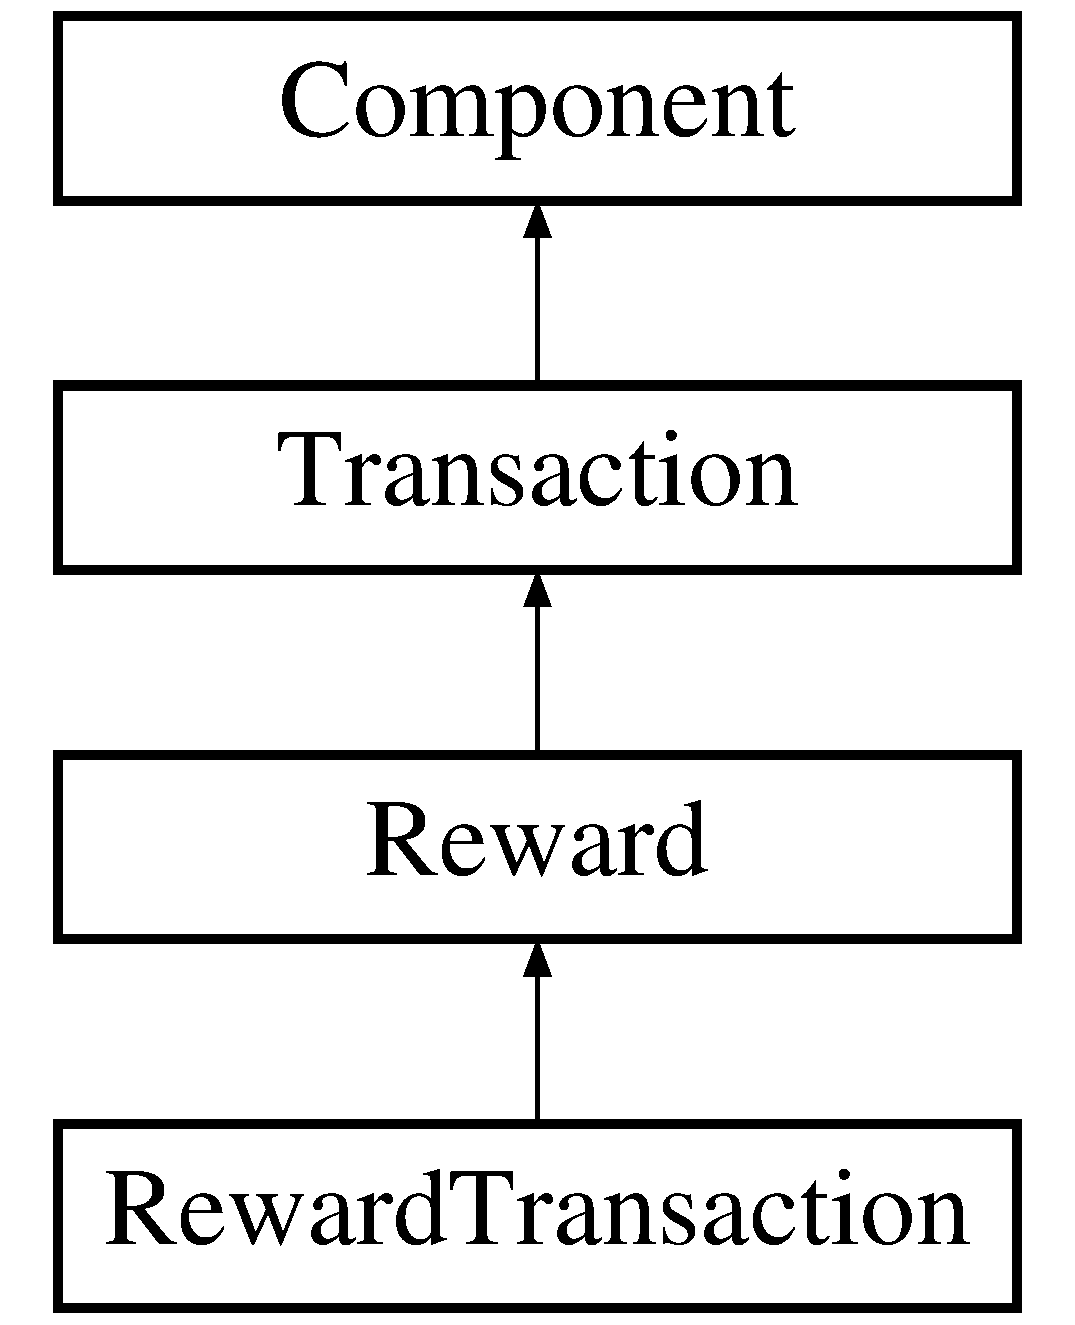
\includegraphics[height=4.000000cm]{classRewardTransaction}
\end{center}
\end{figure}
\subsection*{Public Member Functions}
\begin{DoxyCompactItemize}
\item 
\mbox{\Hypertarget{classRewardTransaction_a414728d857fcf05295a7f3f4fa024dc1}\label{classRewardTransaction_a414728d857fcf05295a7f3f4fa024dc1}} 
\mbox{\hyperlink{classTransaction}{Transaction}} $\ast$ {\bfseries clone} () override
\item 
\mbox{\Hypertarget{classRewardTransaction_ad43c1d706406f40d43f433b0d0b0b510}\label{classRewardTransaction_ad43c1d706406f40d43f433b0d0b0b510}} 
\mbox{\hyperlink{classRow}{Row}} $\ast$ {\bfseries create\+Row} () const override
\item 
\mbox{\Hypertarget{classReward_a1d04370c094170b0d166c341daa1644e}\label{classReward_a1d04370c094170b0d166c341daa1644e}} 
bool {\bfseries operator()} () const final
\item 
\mbox{\Hypertarget{classReward_a0ecd536148463880f9980fe415b6eb1d}\label{classReward_a0ecd536148463880f9980fe415b6eb1d}} 
\mbox{\hyperlink{classElement}{Element}} $\ast$ {\bfseries to\+Element} () const final
\item 
\mbox{\Hypertarget{classReward_ab2cd65f16c670e3e9d8cfe84a6dc56cb}\label{classReward_ab2cd65f16c670e3e9d8cfe84a6dc56cb}} 
bool {\bfseries operator==} (\mbox{\hyperlink{classTransaction}{Transaction}} $\ast$t) const final
\item 
\mbox{\Hypertarget{classReward_a0d65cd39eb260091d1f2cf19e2e71de7}\label{classReward_a0d65cd39eb260091d1f2cf19e2e71de7}} 
std\+::string {\bfseries to\+\_\+string} () const
\item 
\mbox{\Hypertarget{classReward_a494c9d6e0a220729f675fd6131cfb9af}\label{classReward_a494c9d6e0a220729f675fd6131cfb9af}} 
void {\bfseries apply\+\_\+reverse} (\mbox{\hyperlink{classRow}{Row}} $\ast$row) final
\item 
\mbox{\Hypertarget{classReward_a9c9a3219ba6b8b068f7f1cccc779b1b5}\label{classReward_a9c9a3219ba6b8b068f7f1cccc779b1b5}} 
bool {\bfseries validate} (\mbox{\hyperlink{classRow}{Row}} $\ast$row) const final
\item 
\mbox{\Hypertarget{classReward_a1d3d05263d54771a314927d09585968c}\label{classReward_a1d3d05263d54771a314927d09585968c}} 
int {\bfseries get\+\_\+type} () const final
\item 
\mbox{\Hypertarget{classReward_a95e98fc9dbbc9da47cee243adc1932d2}\label{classReward_a95e98fc9dbbc9da47cee243adc1932d2}} 
std\+::string {\bfseries description} () const final
\item 
\mbox{\Hypertarget{classReward_a30a40e2eefd0aea969fab46d1e22d145}\label{classReward_a30a40e2eefd0aea969fab46d1e22d145}} 
void {\bfseries fill\+\_\+data} () final
\item 
\mbox{\Hypertarget{classReward_aae55ec2aa2aa31cc365c80cb42be9ab5}\label{classReward_aae55ec2aa2aa31cc365c80cb42be9ab5}} 
std\+::vector$<$ std\+::string $>$ {\bfseries apply} (\mbox{\hyperlink{classRow}{Row}} $\ast$row) override
\item 
\mbox{\Hypertarget{classTransaction_a1f0df166c34d6a38a991544cf98c0356}\label{classTransaction_a1f0df166c34d6a38a991544cf98c0356}} 
\mbox{\hyperlink{classHash}{Hash}} $\ast$ {\bfseries \+\_\+\+\_\+hash\+\_\+\+\_\+} (const \mbox{\hyperlink{classSerializer}{Serializer}} $\ast$serializer, const char $\ast$encoding) const
\item 
\mbox{\Hypertarget{classComponent_a28212595f8ee85fe009bd233bc99b2fc}\label{classComponent_a28212595f8ee85fe009bd233bc99b2fc}} 
void {\bfseries \+\_\+\+\_\+init\+\_\+\+\_\+} (\mbox{\hyperlink{classElementObject}{Element\+Object}} $\ast$element, const \mbox{\hyperlink{classSerializer}{Serializer}} $\ast$s, const char $\ast$encoding)
\end{DoxyCompactItemize}
\subsection*{Protected Member Functions}
\begin{DoxyCompactItemize}
\item 
\mbox{\Hypertarget{classReward_a6d16e21b60b7f11c7aaf0098a53118a2}\label{classReward_a6d16e21b60b7f11c7aaf0098a53118a2}} 
void {\bfseries from\+Element} (\mbox{\hyperlink{classElementObject}{Element\+Object}} $\ast$, const \mbox{\hyperlink{classSerializer}{Serializer}} $\ast$, const char $\ast$encoding) final
\end{DoxyCompactItemize}


The documentation for this class was generated from the following files\+:\begin{DoxyCompactItemize}
\item 
reward/Reward\+Transaction.\+h\item 
reward/Reward\+Transaction.\+cpp\end{DoxyCompactItemize}

\hypertarget{classRow}{}\section{Row Class Reference}
\label{classRow}\index{Row@{Row}}
Inheritance diagram for Row\+:\begin{figure}[H]
\begin{center}
\leavevmode
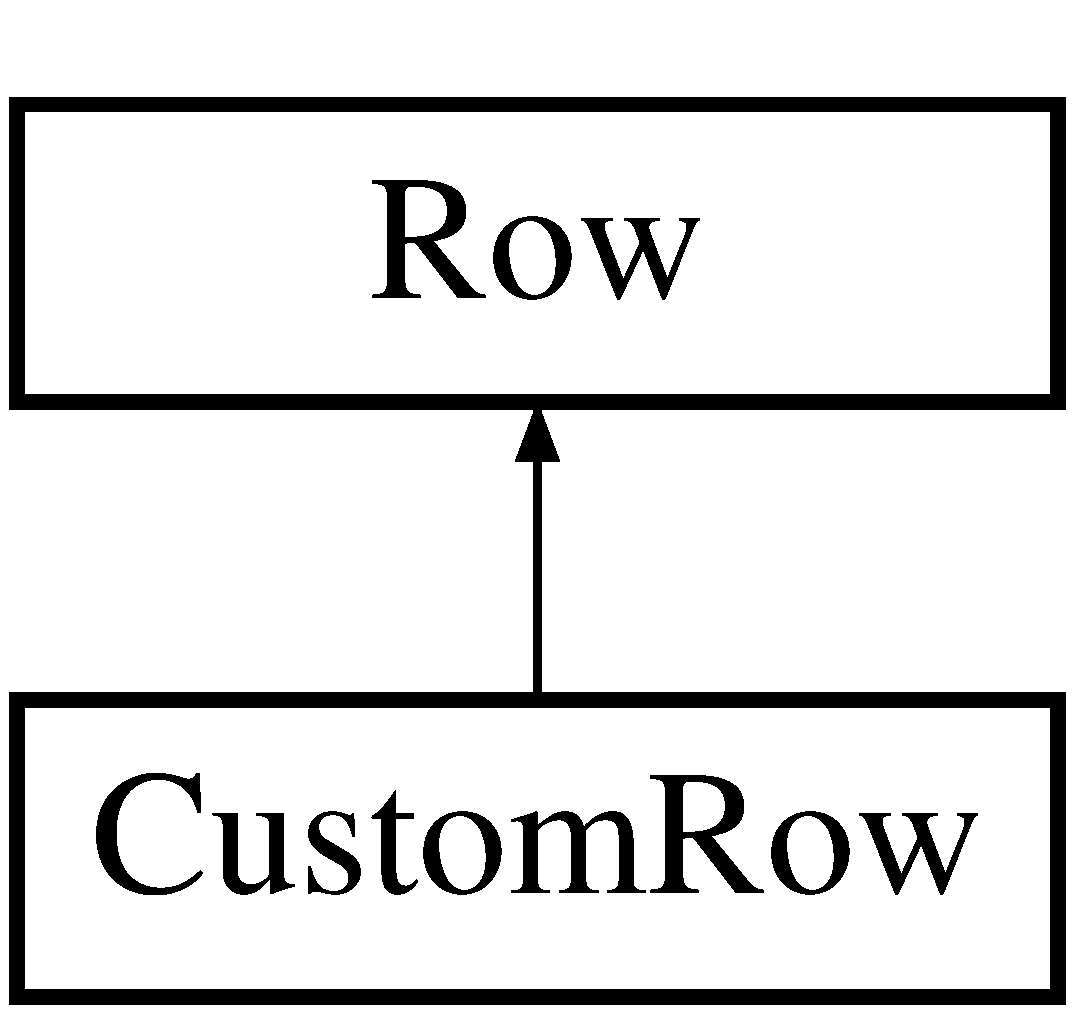
\includegraphics[height=2.000000cm]{classRow}
\end{center}
\end{figure}
\subsection*{Public Member Functions}
\begin{DoxyCompactItemize}
\item 
\mbox{\Hypertarget{classRow_ae3e9c3aaa17ebc4f0e280cdec722440a}\label{classRow_ae3e9c3aaa17ebc4f0e280cdec722440a}} 
virtual \mbox{\hyperlink{classRow}{Row}} $\ast$ {\bfseries clone} () const =0
\item 
\mbox{\Hypertarget{classRow_ae7b1aba7a4c868914700432850c2848d}\label{classRow_ae7b1aba7a4c868914700432850c2848d}} 
virtual std\+::string {\bfseries to\+\_\+string} () const =0
\item 
\mbox{\Hypertarget{classRow_a851b728fa55ecb26f8ebbc87e614581b}\label{classRow_a851b728fa55ecb26f8ebbc87e614581b}} 
virtual void {\bfseries reward} ()=0
\end{DoxyCompactItemize}


The documentation for this class was generated from the following file\+:\begin{DoxyCompactItemize}
\item 
block\+\_\+chain/chain/state/Row.\+h\end{DoxyCompactItemize}

\hypertarget{classRSA__Cryptography}{}\section{R\+S\+A\+\_\+\+Cryptography Class Reference}
\label{classRSA__Cryptography}\index{R\+S\+A\+\_\+\+Cryptography@{R\+S\+A\+\_\+\+Cryptography}}


{\ttfamily \#include $<$R\+S\+A.\+h$>$}

\subsection*{Public Member Functions}
\begin{DoxyCompactItemize}
\item 
\mbox{\hyperlink{classRSA__Cryptography_aeca5b9b416a49fea20e7fc69ca18d641}{R\+S\+A\+\_\+\+Cryptography}} ()
\item 
\mbox{\hyperlink{classRSA__Cryptography_ae2cd6fb565102dc8007de9d305026e45}{R\+S\+A\+\_\+\+Cryptography}} (std\+::string key)
\item 
std\+::string \mbox{\hyperlink{classRSA__Cryptography_a8ea8d421dcb5012ffc8fd23660bae1bc}{encrypt}} (std\+::string message)
\item 
std\+::string \mbox{\hyperlink{classRSA__Cryptography_a03760e4f7eae8e7b961f8b948c0dafb1}{decrypt}} (std\+::string message, int size)
\item 
void \mbox{\hyperlink{classRSA__Cryptography_a7772b886bb2f27b95df33019d04eee69}{write}} (void($\ast$fun)(B\+IO $\ast$, R\+SA $\ast$), std\+::string file)
\item 
std\+::string \mbox{\hyperlink{classRSA__Cryptography_a9692bde79db1e43da95511fe0d0c1a0b}{get\+Public\+Key}} ()
\item 
std\+::string \mbox{\hyperlink{classRSA__Cryptography_aecdd6715cb222a98b5810f49103c34d7}{get\+Private\+Key}} ()
\item 
void \mbox{\hyperlink{classRSA__Cryptography_aaf500fcdcc050fa8d18a0dbe43176d17}{generate}} (const char $\ast$private\+\_\+file, const char $\ast$public\+\_\+file)
\item 
bool \mbox{\hyperlink{classRSA__Cryptography_ae3ccf77d8754acdfb444dbab6fb6a4dd}{backup}} (const char $\ast$private\+\_\+file, const char $\ast$public\+\_\+file)
\item 
virtual \mbox{\hyperlink{classRSA__Cryptography_ae8a837cfb0a55afd707af939261acc52}{$\sim$\+R\+S\+A\+\_\+\+Cryptography}} ()
\end{DoxyCompactItemize}


\subsection{Detailed Description}
A class for R\+SA cryptography, based on Open\+S\+LL

\begin{DoxyAuthor}{Author}
Mathieu Lochet 
\end{DoxyAuthor}
\begin{DoxyVersion}{Version}
2 
\end{DoxyVersion}


\subsection{Constructor \& Destructor Documentation}
\mbox{\Hypertarget{classRSA__Cryptography_aeca5b9b416a49fea20e7fc69ca18d641}\label{classRSA__Cryptography_aeca5b9b416a49fea20e7fc69ca18d641}} 
\index{R\+S\+A\+\_\+\+Cryptography@{R\+S\+A\+\_\+\+Cryptography}!R\+S\+A\+\_\+\+Cryptography@{R\+S\+A\+\_\+\+Cryptography}}
\index{R\+S\+A\+\_\+\+Cryptography@{R\+S\+A\+\_\+\+Cryptography}!R\+S\+A\+\_\+\+Cryptography@{R\+S\+A\+\_\+\+Cryptography}}
\subsubsection{\texorpdfstring{R\+S\+A\+\_\+\+Cryptography()}{RSA\_Cryptography()}\hspace{0.1cm}{\footnotesize\ttfamily [1/2]}}
{\footnotesize\ttfamily R\+S\+A\+\_\+\+Cryptography\+::\+R\+S\+A\+\_\+\+Cryptography (\begin{DoxyParamCaption}{ }\end{DoxyParamCaption})}

A default constructor initializing the size of the key \mbox{\Hypertarget{classRSA__Cryptography_ae2cd6fb565102dc8007de9d305026e45}\label{classRSA__Cryptography_ae2cd6fb565102dc8007de9d305026e45}} 
\index{R\+S\+A\+\_\+\+Cryptography@{R\+S\+A\+\_\+\+Cryptography}!R\+S\+A\+\_\+\+Cryptography@{R\+S\+A\+\_\+\+Cryptography}}
\index{R\+S\+A\+\_\+\+Cryptography@{R\+S\+A\+\_\+\+Cryptography}!R\+S\+A\+\_\+\+Cryptography@{R\+S\+A\+\_\+\+Cryptography}}
\subsubsection{\texorpdfstring{R\+S\+A\+\_\+\+Cryptography()}{RSA\_Cryptography()}\hspace{0.1cm}{\footnotesize\ttfamily [2/2]}}
{\footnotesize\ttfamily R\+S\+A\+\_\+\+Cryptography\+::\+R\+S\+A\+\_\+\+Cryptography (\begin{DoxyParamCaption}\item[{std\+::string}]{key }\end{DoxyParamCaption})\hspace{0.3cm}{\ttfamily [explicit]}}

A constructor with a given public key. It creates an object that can decrypt or encrypt using public key


\begin{DoxyParams}{Parameters}
{\em key} & The known public key \\
\hline
\end{DoxyParams}
\mbox{\Hypertarget{classRSA__Cryptography_ae8a837cfb0a55afd707af939261acc52}\label{classRSA__Cryptography_ae8a837cfb0a55afd707af939261acc52}} 
\index{R\+S\+A\+\_\+\+Cryptography@{R\+S\+A\+\_\+\+Cryptography}!````~R\+S\+A\+\_\+\+Cryptography@{$\sim$\+R\+S\+A\+\_\+\+Cryptography}}
\index{````~R\+S\+A\+\_\+\+Cryptography@{$\sim$\+R\+S\+A\+\_\+\+Cryptography}!R\+S\+A\+\_\+\+Cryptography@{R\+S\+A\+\_\+\+Cryptography}}
\subsubsection{\texorpdfstring{$\sim$\+R\+S\+A\+\_\+\+Cryptography()}{~RSA\_Cryptography()}}
{\footnotesize\ttfamily R\+S\+A\+\_\+\+Cryptography\+::$\sim$\+R\+S\+A\+\_\+\+Cryptography (\begin{DoxyParamCaption}{ }\end{DoxyParamCaption})\hspace{0.3cm}{\ttfamily [virtual]}}

Frees R\+SA key ressources 

\subsection{Member Function Documentation}
\mbox{\Hypertarget{classRSA__Cryptography_ae3ccf77d8754acdfb444dbab6fb6a4dd}\label{classRSA__Cryptography_ae3ccf77d8754acdfb444dbab6fb6a4dd}} 
\index{R\+S\+A\+\_\+\+Cryptography@{R\+S\+A\+\_\+\+Cryptography}!backup@{backup}}
\index{backup@{backup}!R\+S\+A\+\_\+\+Cryptography@{R\+S\+A\+\_\+\+Cryptography}}
\subsubsection{\texorpdfstring{backup()}{backup()}}
{\footnotesize\ttfamily bool R\+S\+A\+\_\+\+Cryptography\+::backup (\begin{DoxyParamCaption}\item[{const char $\ast$}]{private\+\_\+file,  }\item[{const char $\ast$}]{public\+\_\+file }\end{DoxyParamCaption})}

Read the key from files


\begin{DoxyParams}{Parameters}
{\em private\+\_\+file} & The file in which to read the private key \\
\hline
{\em public\+\_\+file} & The file in which to read the public key \\
\hline
\end{DoxyParams}
\mbox{\Hypertarget{classRSA__Cryptography_a03760e4f7eae8e7b961f8b948c0dafb1}\label{classRSA__Cryptography_a03760e4f7eae8e7b961f8b948c0dafb1}} 
\index{R\+S\+A\+\_\+\+Cryptography@{R\+S\+A\+\_\+\+Cryptography}!decrypt@{decrypt}}
\index{decrypt@{decrypt}!R\+S\+A\+\_\+\+Cryptography@{R\+S\+A\+\_\+\+Cryptography}}
\subsubsection{\texorpdfstring{decrypt()}{decrypt()}}
{\footnotesize\ttfamily std\+::string R\+S\+A\+\_\+\+Cryptography\+::decrypt (\begin{DoxyParamCaption}\item[{std\+::string}]{message,  }\item[{int}]{size }\end{DoxyParamCaption})}

Decrypt a message using private key


\begin{DoxyParams}{Parameters}
{\em message} & The message to decrypt \\
\hline
{\em size} & The size of the message to decrypt \\
\hline
\end{DoxyParams}
\begin{DoxyReturn}{Returns}
The decrypted message 
\end{DoxyReturn}
\mbox{\Hypertarget{classRSA__Cryptography_a8ea8d421dcb5012ffc8fd23660bae1bc}\label{classRSA__Cryptography_a8ea8d421dcb5012ffc8fd23660bae1bc}} 
\index{R\+S\+A\+\_\+\+Cryptography@{R\+S\+A\+\_\+\+Cryptography}!encrypt@{encrypt}}
\index{encrypt@{encrypt}!R\+S\+A\+\_\+\+Cryptography@{R\+S\+A\+\_\+\+Cryptography}}
\subsubsection{\texorpdfstring{encrypt()}{encrypt()}}
{\footnotesize\ttfamily std\+::string R\+S\+A\+\_\+\+Cryptography\+::encrypt (\begin{DoxyParamCaption}\item[{std\+::string}]{message }\end{DoxyParamCaption})}

Encrypt a message using private key


\begin{DoxyParams}{Parameters}
{\em message} & The message to encrypt \\
\hline
\end{DoxyParams}
\begin{DoxyReturn}{Returns}
The encrypted message 
\end{DoxyReturn}
\mbox{\Hypertarget{classRSA__Cryptography_aaf500fcdcc050fa8d18a0dbe43176d17}\label{classRSA__Cryptography_aaf500fcdcc050fa8d18a0dbe43176d17}} 
\index{R\+S\+A\+\_\+\+Cryptography@{R\+S\+A\+\_\+\+Cryptography}!generate@{generate}}
\index{generate@{generate}!R\+S\+A\+\_\+\+Cryptography@{R\+S\+A\+\_\+\+Cryptography}}
\subsubsection{\texorpdfstring{generate()}{generate()}}
{\footnotesize\ttfamily void R\+S\+A\+\_\+\+Cryptography\+::generate (\begin{DoxyParamCaption}\item[{const char $\ast$}]{private\+\_\+file,  }\item[{const char $\ast$}]{public\+\_\+file }\end{DoxyParamCaption})}

Generates new R\+SA key and writes it into a file


\begin{DoxyParams}{Parameters}
{\em private\+\_\+file} & The file in which to write the private key \\
\hline
{\em public\+\_\+file} & The file in which to write the public key \\
\hline
\end{DoxyParams}
\mbox{\Hypertarget{classRSA__Cryptography_aecdd6715cb222a98b5810f49103c34d7}\label{classRSA__Cryptography_aecdd6715cb222a98b5810f49103c34d7}} 
\index{R\+S\+A\+\_\+\+Cryptography@{R\+S\+A\+\_\+\+Cryptography}!get\+Private\+Key@{get\+Private\+Key}}
\index{get\+Private\+Key@{get\+Private\+Key}!R\+S\+A\+\_\+\+Cryptography@{R\+S\+A\+\_\+\+Cryptography}}
\subsubsection{\texorpdfstring{get\+Private\+Key()}{getPrivateKey()}}
{\footnotesize\ttfamily std\+::string R\+S\+A\+\_\+\+Cryptography\+::get\+Private\+Key (\begin{DoxyParamCaption}{ }\end{DoxyParamCaption})}

Get the private key

\begin{DoxyReturn}{Returns}
The private key 
\end{DoxyReturn}
\mbox{\Hypertarget{classRSA__Cryptography_a9692bde79db1e43da95511fe0d0c1a0b}\label{classRSA__Cryptography_a9692bde79db1e43da95511fe0d0c1a0b}} 
\index{R\+S\+A\+\_\+\+Cryptography@{R\+S\+A\+\_\+\+Cryptography}!get\+Public\+Key@{get\+Public\+Key}}
\index{get\+Public\+Key@{get\+Public\+Key}!R\+S\+A\+\_\+\+Cryptography@{R\+S\+A\+\_\+\+Cryptography}}
\subsubsection{\texorpdfstring{get\+Public\+Key()}{getPublicKey()}}
{\footnotesize\ttfamily std\+::string R\+S\+A\+\_\+\+Cryptography\+::get\+Public\+Key (\begin{DoxyParamCaption}{ }\end{DoxyParamCaption})}

Get the public key

\begin{DoxyReturn}{Returns}
The public key 
\end{DoxyReturn}
\mbox{\Hypertarget{classRSA__Cryptography_a7772b886bb2f27b95df33019d04eee69}\label{classRSA__Cryptography_a7772b886bb2f27b95df33019d04eee69}} 
\index{R\+S\+A\+\_\+\+Cryptography@{R\+S\+A\+\_\+\+Cryptography}!write@{write}}
\index{write@{write}!R\+S\+A\+\_\+\+Cryptography@{R\+S\+A\+\_\+\+Cryptography}}
\subsubsection{\texorpdfstring{write()}{write()}}
{\footnotesize\ttfamily void R\+S\+A\+\_\+\+Cryptography\+::write (\begin{DoxyParamCaption}\item[{void($\ast$)(B\+IO $\ast$, R\+SA $\ast$)}]{fun,  }\item[{std\+::string}]{file }\end{DoxyParamCaption})}

Write a key inside a file


\begin{DoxyParams}{Parameters}
{\em fun} & The function that will choose which key to write \\
\hline
{\em file} & The file name \\
\hline
\end{DoxyParams}


The documentation for this class was generated from the following files\+:\begin{DoxyCompactItemize}
\item 
block\+\_\+chain/algorithm/R\+S\+A.\+h\item 
block\+\_\+chain/algorithm/R\+S\+A.\+cpp\end{DoxyCompactItemize}

\hypertarget{classSerializer}{}\section{Serializer Class Reference}
\label{classSerializer}\index{Serializer@{Serializer}}


{\ttfamily \#include $<$Serializer.\+h$>$}

Inheritance diagram for Serializer\+:\begin{figure}[H]
\begin{center}
\leavevmode
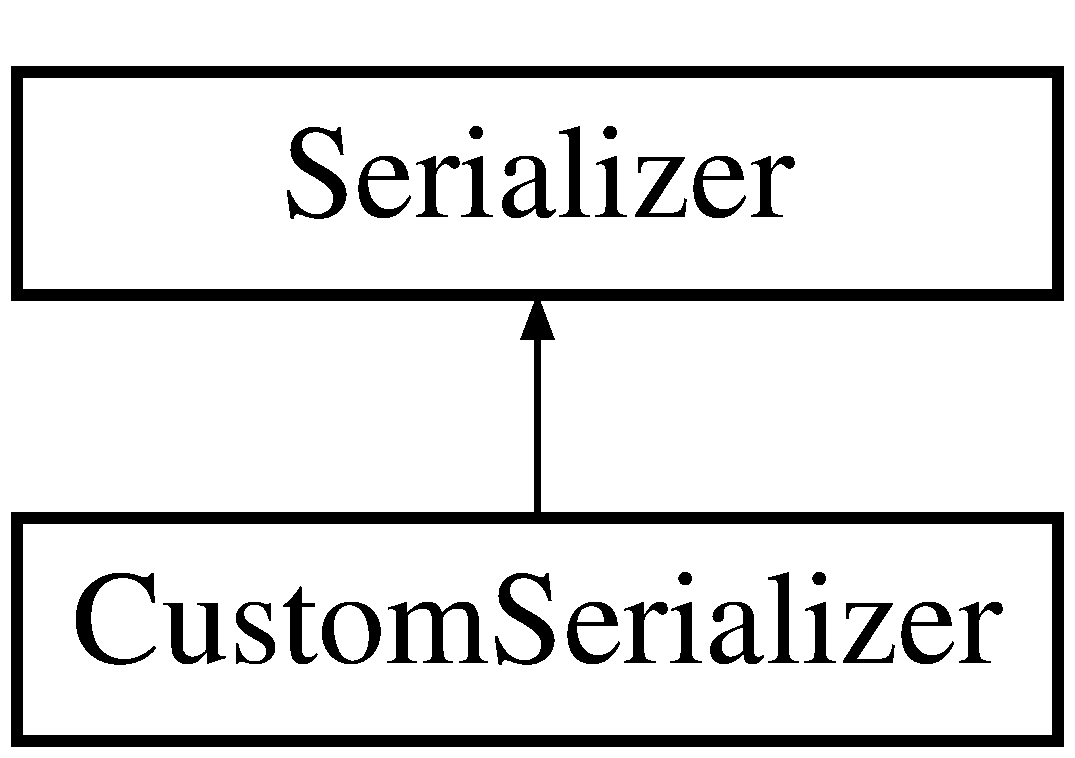
\includegraphics[height=2.000000cm]{classSerializer}
\end{center}
\end{figure}
\subsection*{Public Member Functions}
\begin{DoxyCompactItemize}
\item 
\mbox{\hyperlink{classSerializer_a9fe7f31924098f75278d059f8443fd5b}{Serializer}} ()
\item 
virtual \mbox{\hyperlink{classSerializer_a42a7d2d8e622ad1ef5f869813b498aa9}{$\sim$\+Serializer}} ()
\item 
virtual char $\ast$ \mbox{\hyperlink{classSerializer_a5cfe31eb70f4d0c92f2d68c22f39e885}{serialize}} (const \mbox{\hyperlink{classComponent}{Component}} $\ast$component, const char $\ast$encoding) const
\item 
virtual char $\ast$ \mbox{\hyperlink{classSerializer_a38bec517fb3b3cc0778c75b807cb930c}{serialize}} (\mbox{\hyperlink{classElement}{Element}} $\ast$element, const char $\ast$encoding) const
\item 
virtual \mbox{\hyperlink{classTransaction}{Transaction}} $\ast$ \mbox{\hyperlink{classSerializer_ab5fa979a8486be6f49ad10f4810509d7}{unserialize\+Transaction}} (std\+::string transaction, const char $\ast$encoding) const
\item 
virtual \mbox{\hyperlink{classBlock}{Block}} $\ast$ \mbox{\hyperlink{classSerializer_a423fb7c43ca9c23e07000dba0c5a432a}{unserialize\+Block}} (std\+::string block, const char $\ast$encoding) const
\item 
virtual \mbox{\hyperlink{classMessage}{Message}} $\ast$ \mbox{\hyperlink{classSerializer_a1d16df9f35a7580da06a497dfbddffe8}{unserialize\+Message}} (std\+::string message, const char $\ast$encoding) const
\item 
virtual \mbox{\hyperlink{classMetadata}{Metadata}} $\ast$ \mbox{\hyperlink{classSerializer_a64b858f0c2968e888cf796b6f09eed7b}{unserialize\+Metadata}} (std\+::string message, const char $\ast$encoding) const
\item 
\mbox{\hyperlink{classElementObject}{Element\+Object}} $\ast$ \mbox{\hyperlink{classSerializer_ab3bcdbd49167109de13e03878337018a}{get\+Element}} (std\+::string str, const char $\ast$encoding) const
\item 
void \mbox{\hyperlink{classSerializer_aee483f1845ca1b7f7ac4243de9902750}{set\+\_\+serializer}} (\mbox{\hyperlink{classContentCreator}{Content\+Creator}} $\ast$creator)
\item 
void \mbox{\hyperlink{classSerializer_a74ea868b820b4a8472da98c0045418fa}{set\+\_\+unserializer}} (\mbox{\hyperlink{classContentParser}{Content\+Parser}} $\ast$parser)
\end{DoxyCompactItemize}
\subsection*{Protected Attributes}
\begin{DoxyCompactItemize}
\item 
\mbox{\hyperlink{classFactory}{Factory}}$<$ \mbox{\hyperlink{classContentCreator}{Content\+Creator}} $\ast$ $>$ \mbox{\hyperlink{classSerializer_a7d26e865966b304350653b1246ec3340}{creators}}
\item 
\mbox{\hyperlink{classFactory}{Factory}}$<$ \mbox{\hyperlink{classContentParser}{Content\+Parser}} $\ast$ $>$ \mbox{\hyperlink{classSerializer_a96f96c01e6a471513669621751591fd9}{parsers}}
\end{DoxyCompactItemize}


\subsection{Detailed Description}
An abstract serializer. The class \mbox{\hyperlink{classSerializer}{Serializer}} implements almost all of the serialization and unserialization methods. However, it doesn\textquotesingle{}t implements the transaction unserialization, therefore, this class has to be override. \begin{DoxySeeAlso}{See also}
\mbox{\hyperlink{classContentCreator}{Content\+Creator}} 

\mbox{\hyperlink{classContentParser}{Content\+Parser}} 

\mbox{\hyperlink{classElement}{Element}} 

\mbox{\hyperlink{classElementObject}{Element\+Object}} 

\mbox{\hyperlink{classComponent}{Component}} 

\mbox{\hyperlink{classTransaction}{Transaction}} 

\mbox{\hyperlink{classBlock}{Block}} 

\mbox{\hyperlink{classMessage}{Message}} 

\mbox{\hyperlink{classMetadata}{Metadata}}
\end{DoxySeeAlso}
\begin{DoxyAuthor}{Author}
Mathieu Lochet 
\end{DoxyAuthor}
\begin{DoxyVersion}{Version}
3 
\end{DoxyVersion}


\subsection{Constructor \& Destructor Documentation}
\mbox{\Hypertarget{classSerializer_a9fe7f31924098f75278d059f8443fd5b}\label{classSerializer_a9fe7f31924098f75278d059f8443fd5b}} 
\index{Serializer@{Serializer}!Serializer@{Serializer}}
\index{Serializer@{Serializer}!Serializer@{Serializer}}
\subsubsection{\texorpdfstring{Serializer()}{Serializer()}}
{\footnotesize\ttfamily Serializer\+::\+Serializer (\begin{DoxyParamCaption}{ }\end{DoxyParamCaption})}

Initialize the \mbox{\hyperlink{classSerializer}{Serializer}} with default readers\+:
\begin{DoxyItemize}
\item json creator
\item json parser They can be used as encoding \begin{DoxySeeAlso}{See also}
\mbox{\hyperlink{classJsonCreator}{Json\+Creator}} 

\mbox{\hyperlink{classJsonParser}{Json\+Parser}} 
\end{DoxySeeAlso}

\end{DoxyItemize}\mbox{\Hypertarget{classSerializer_a42a7d2d8e622ad1ef5f869813b498aa9}\label{classSerializer_a42a7d2d8e622ad1ef5f869813b498aa9}} 
\index{Serializer@{Serializer}!````~Serializer@{$\sim$\+Serializer}}
\index{````~Serializer@{$\sim$\+Serializer}!Serializer@{Serializer}}
\subsubsection{\texorpdfstring{$\sim$\+Serializer()}{~Serializer()}}
{\footnotesize\ttfamily Serializer\+::$\sim$\+Serializer (\begin{DoxyParamCaption}{ }\end{DoxyParamCaption})\hspace{0.3cm}{\ttfamily [virtual]}}

Default destructor that clears the factories 

\subsection{Member Function Documentation}
\mbox{\Hypertarget{classSerializer_ab3bcdbd49167109de13e03878337018a}\label{classSerializer_ab3bcdbd49167109de13e03878337018a}} 
\index{Serializer@{Serializer}!get\+Element@{get\+Element}}
\index{get\+Element@{get\+Element}!Serializer@{Serializer}}
\subsubsection{\texorpdfstring{get\+Element()}{getElement()}}
{\footnotesize\ttfamily \mbox{\hyperlink{classElementObject}{Element\+Object}} $\ast$ Serializer\+::get\+Element (\begin{DoxyParamCaption}\item[{std\+::string}]{str,  }\item[{const char $\ast$}]{encoding }\end{DoxyParamCaption}) const}

Unserialize a given string to obtain a \mbox{\hyperlink{classMetadata}{Metadata}} \begin{DoxySeeAlso}{See also}
\mbox{\hyperlink{classContentParser}{Content\+Parser}} 

\mbox{\hyperlink{classElementObject}{Element\+Object}}
\end{DoxySeeAlso}

\begin{DoxyParams}{Parameters}
{\em str} & the string to be unserialized \\
\hline
{\em encoding} & the key to choose the parser \\
\hline
\end{DoxyParams}
\begin{DoxyReturn}{Returns}
The \mbox{\hyperlink{classElement}{Element}} representation of the string 
\end{DoxyReturn}
\mbox{\Hypertarget{classSerializer_a5cfe31eb70f4d0c92f2d68c22f39e885}\label{classSerializer_a5cfe31eb70f4d0c92f2d68c22f39e885}} 
\index{Serializer@{Serializer}!serialize@{serialize}}
\index{serialize@{serialize}!Serializer@{Serializer}}
\subsubsection{\texorpdfstring{serialize()}{serialize()}\hspace{0.1cm}{\footnotesize\ttfamily [1/2]}}
{\footnotesize\ttfamily char $\ast$ Serializer\+::serialize (\begin{DoxyParamCaption}\item[{const \mbox{\hyperlink{classComponent}{Component}} $\ast$}]{component,  }\item[{const char $\ast$}]{encoding }\end{DoxyParamCaption}) const\hspace{0.3cm}{\ttfamily [virtual]}}

Serialize a \mbox{\hyperlink{classComponent}{Component}} object \begin{DoxySeeAlso}{See also}
\mbox{\hyperlink{classComponent}{Component}} 

\mbox{\hyperlink{classContentCreator}{Content\+Creator}}
\end{DoxySeeAlso}

\begin{DoxyParams}{Parameters}
{\em component} & the component to be serialized \\
\hline
{\em encoding} & the key to choose the creator \\
\hline
\end{DoxyParams}
\begin{DoxyReturn}{Returns}
the serialized string 
\end{DoxyReturn}
\mbox{\Hypertarget{classSerializer_a38bec517fb3b3cc0778c75b807cb930c}\label{classSerializer_a38bec517fb3b3cc0778c75b807cb930c}} 
\index{Serializer@{Serializer}!serialize@{serialize}}
\index{serialize@{serialize}!Serializer@{Serializer}}
\subsubsection{\texorpdfstring{serialize()}{serialize()}\hspace{0.1cm}{\footnotesize\ttfamily [2/2]}}
{\footnotesize\ttfamily char $\ast$ Serializer\+::serialize (\begin{DoxyParamCaption}\item[{\mbox{\hyperlink{classElement}{Element}} $\ast$}]{element,  }\item[{const char $\ast$}]{encoding }\end{DoxyParamCaption}) const\hspace{0.3cm}{\ttfamily [virtual]}}

Serialize an \mbox{\hyperlink{classElement}{Element}} object \begin{DoxySeeAlso}{See also}
\mbox{\hyperlink{classElement}{Element}} 

\mbox{\hyperlink{classContentCreator}{Content\+Creator}}
\end{DoxySeeAlso}

\begin{DoxyParams}{Parameters}
{\em element} & the element to be serialized \\
\hline
{\em encoding} & the key to choose the creator \\
\hline
\end{DoxyParams}
\begin{DoxyReturn}{Returns}
the serialized string 
\end{DoxyReturn}
\mbox{\Hypertarget{classSerializer_aee483f1845ca1b7f7ac4243de9902750}\label{classSerializer_aee483f1845ca1b7f7ac4243de9902750}} 
\index{Serializer@{Serializer}!set\+\_\+serializer@{set\+\_\+serializer}}
\index{set\+\_\+serializer@{set\+\_\+serializer}!Serializer@{Serializer}}
\subsubsection{\texorpdfstring{set\+\_\+serializer()}{set\_serializer()}}
{\footnotesize\ttfamily void Serializer\+::set\+\_\+serializer (\begin{DoxyParamCaption}\item[{\mbox{\hyperlink{classContentCreator}{Content\+Creator}} $\ast$}]{creator }\end{DoxyParamCaption})}

Add a custom creator to the list \begin{DoxySeeAlso}{See also}
\mbox{\hyperlink{classContentCreator}{Content\+Creator}}
\end{DoxySeeAlso}

\begin{DoxyParams}{Parameters}
{\em creator} & the creator object to use \\
\hline
\end{DoxyParams}
\mbox{\Hypertarget{classSerializer_a74ea868b820b4a8472da98c0045418fa}\label{classSerializer_a74ea868b820b4a8472da98c0045418fa}} 
\index{Serializer@{Serializer}!set\+\_\+unserializer@{set\+\_\+unserializer}}
\index{set\+\_\+unserializer@{set\+\_\+unserializer}!Serializer@{Serializer}}
\subsubsection{\texorpdfstring{set\+\_\+unserializer()}{set\_unserializer()}}
{\footnotesize\ttfamily void Serializer\+::set\+\_\+unserializer (\begin{DoxyParamCaption}\item[{\mbox{\hyperlink{classContentParser}{Content\+Parser}} $\ast$}]{parser }\end{DoxyParamCaption})}

Add a custom parser to the list \begin{DoxySeeAlso}{See also}
\mbox{\hyperlink{classContentParser}{Content\+Parser}}
\end{DoxySeeAlso}

\begin{DoxyParams}{Parameters}
{\em creator} & the parser object \\
\hline
\end{DoxyParams}
\mbox{\Hypertarget{classSerializer_a423fb7c43ca9c23e07000dba0c5a432a}\label{classSerializer_a423fb7c43ca9c23e07000dba0c5a432a}} 
\index{Serializer@{Serializer}!unserialize\+Block@{unserialize\+Block}}
\index{unserialize\+Block@{unserialize\+Block}!Serializer@{Serializer}}
\subsubsection{\texorpdfstring{unserialize\+Block()}{unserializeBlock()}}
{\footnotesize\ttfamily \mbox{\hyperlink{classBlock}{Block}} $\ast$ Serializer\+::unserialize\+Block (\begin{DoxyParamCaption}\item[{std\+::string}]{block,  }\item[{const char $\ast$}]{encoding }\end{DoxyParamCaption}) const\hspace{0.3cm}{\ttfamily [virtual]}}

Unserialize an given string to obtain a \mbox{\hyperlink{classBlock}{Block}} \begin{DoxySeeAlso}{See also}
\mbox{\hyperlink{classContentParser}{Content\+Parser}} 

\mbox{\hyperlink{classBlock}{Block}}
\end{DoxySeeAlso}

\begin{DoxyParams}{Parameters}
{\em block} & the string to be unserialized \\
\hline
{\em encoding} & the key to choose the parser \\
\hline
\end{DoxyParams}
\begin{DoxyReturn}{Returns}
The \mbox{\hyperlink{classBlock}{Block}} object 
\end{DoxyReturn}
\mbox{\Hypertarget{classSerializer_a1d16df9f35a7580da06a497dfbddffe8}\label{classSerializer_a1d16df9f35a7580da06a497dfbddffe8}} 
\index{Serializer@{Serializer}!unserialize\+Message@{unserialize\+Message}}
\index{unserialize\+Message@{unserialize\+Message}!Serializer@{Serializer}}
\subsubsection{\texorpdfstring{unserialize\+Message()}{unserializeMessage()}}
{\footnotesize\ttfamily \mbox{\hyperlink{classMessage}{Message}} $\ast$ Serializer\+::unserialize\+Message (\begin{DoxyParamCaption}\item[{std\+::string}]{message,  }\item[{const char $\ast$}]{encoding }\end{DoxyParamCaption}) const\hspace{0.3cm}{\ttfamily [virtual]}}

Unserialize an given string to obtain a \mbox{\hyperlink{classMessage}{Message}} \begin{DoxySeeAlso}{See also}
\mbox{\hyperlink{classContentParser}{Content\+Parser}} 

\mbox{\hyperlink{classMessage}{Message}}
\end{DoxySeeAlso}

\begin{DoxyParams}{Parameters}
{\em message} & the string to be unserialized \\
\hline
{\em encoding} & the key to choose the parser \\
\hline
\end{DoxyParams}
\begin{DoxyReturn}{Returns}
The \mbox{\hyperlink{classMessage}{Message}} object 
\end{DoxyReturn}
\mbox{\Hypertarget{classSerializer_a64b858f0c2968e888cf796b6f09eed7b}\label{classSerializer_a64b858f0c2968e888cf796b6f09eed7b}} 
\index{Serializer@{Serializer}!unserialize\+Metadata@{unserialize\+Metadata}}
\index{unserialize\+Metadata@{unserialize\+Metadata}!Serializer@{Serializer}}
\subsubsection{\texorpdfstring{unserialize\+Metadata()}{unserializeMetadata()}}
{\footnotesize\ttfamily \mbox{\hyperlink{classMetadata}{Metadata}} $\ast$ Serializer\+::unserialize\+Metadata (\begin{DoxyParamCaption}\item[{std\+::string}]{message,  }\item[{const char $\ast$}]{encoding }\end{DoxyParamCaption}) const\hspace{0.3cm}{\ttfamily [virtual]}}

Unserialize an given string to obtain a \mbox{\hyperlink{classMetadata}{Metadata}} \begin{DoxySeeAlso}{See also}
\mbox{\hyperlink{classContentParser}{Content\+Parser}} 

\mbox{\hyperlink{classMetadata}{Metadata}}
\end{DoxySeeAlso}

\begin{DoxyParams}{Parameters}
{\em message} & the string to be unserialized \\
\hline
{\em encoding} & the key to choose the parser \\
\hline
\end{DoxyParams}
\begin{DoxyReturn}{Returns}
The \mbox{\hyperlink{classMetadata}{Metadata}} object 
\end{DoxyReturn}
\mbox{\Hypertarget{classSerializer_ab5fa979a8486be6f49ad10f4810509d7}\label{classSerializer_ab5fa979a8486be6f49ad10f4810509d7}} 
\index{Serializer@{Serializer}!unserialize\+Transaction@{unserialize\+Transaction}}
\index{unserialize\+Transaction@{unserialize\+Transaction}!Serializer@{Serializer}}
\subsubsection{\texorpdfstring{unserialize\+Transaction()}{unserializeTransaction()}}
{\footnotesize\ttfamily \mbox{\hyperlink{classTransaction}{Transaction}} $\ast$ Serializer\+::unserialize\+Transaction (\begin{DoxyParamCaption}\item[{std\+::string}]{transaction,  }\item[{const char $\ast$}]{encoding }\end{DoxyParamCaption}) const\hspace{0.3cm}{\ttfamily [virtual]}}

Unserialize an given string to obtain a \mbox{\hyperlink{classTransaction}{Transaction}} (needs override) \begin{DoxySeeAlso}{See also}
\mbox{\hyperlink{classContentParser}{Content\+Parser}} 

\mbox{\hyperlink{classTransaction}{Transaction}}
\end{DoxySeeAlso}

\begin{DoxyParams}{Parameters}
{\em transaction} & the string to be unserialized \\
\hline
{\em encoding} & the key to choose the parser \\
\hline
\end{DoxyParams}
\begin{DoxyReturn}{Returns}
The \mbox{\hyperlink{classTransaction}{Transaction}} object 
\end{DoxyReturn}


Reimplemented in \mbox{\hyperlink{classCustomSerializer_abff58f1a955c2f399127b7e3cae23223}{Custom\+Serializer}}.



\subsection{Member Data Documentation}
\mbox{\Hypertarget{classSerializer_a7d26e865966b304350653b1246ec3340}\label{classSerializer_a7d26e865966b304350653b1246ec3340}} 
\index{Serializer@{Serializer}!creators@{creators}}
\index{creators@{creators}!Serializer@{Serializer}}
\subsubsection{\texorpdfstring{creators}{creators}}
{\footnotesize\ttfamily \mbox{\hyperlink{classFactory}{Factory}}$<$\mbox{\hyperlink{classContentCreator}{Content\+Creator}}$\ast$$>$ Serializer\+::creators\hspace{0.3cm}{\ttfamily [protected]}}

The factory of different creators \begin{DoxySeeAlso}{See also}
\mbox{\hyperlink{classFactory}{Factory}} 

\mbox{\hyperlink{classContentCreator}{Content\+Creator}} 
\end{DoxySeeAlso}
\mbox{\Hypertarget{classSerializer_a96f96c01e6a471513669621751591fd9}\label{classSerializer_a96f96c01e6a471513669621751591fd9}} 
\index{Serializer@{Serializer}!parsers@{parsers}}
\index{parsers@{parsers}!Serializer@{Serializer}}
\subsubsection{\texorpdfstring{parsers}{parsers}}
{\footnotesize\ttfamily \mbox{\hyperlink{classFactory}{Factory}}$<$\mbox{\hyperlink{classContentParser}{Content\+Parser}}$\ast$$>$ Serializer\+::parsers\hspace{0.3cm}{\ttfamily [protected]}}

The factory of different parsers \begin{DoxySeeAlso}{See also}
\mbox{\hyperlink{classFactory}{Factory}} 

\mbox{\hyperlink{classContentParser}{Content\+Parser}} 
\end{DoxySeeAlso}


The documentation for this class was generated from the following files\+:\begin{DoxyCompactItemize}
\item 
block\+\_\+chain/utils/serialization/Serializer.\+h\item 
block\+\_\+chain/utils/serialization/Serializer.\+cpp\end{DoxyCompactItemize}

\hypertarget{classSignInMessage}{}\section{Sign\+In\+Message Class Reference}
\label{classSignInMessage}\index{Sign\+In\+Message@{Sign\+In\+Message}}
Inheritance diagram for Sign\+In\+Message\+:\begin{figure}[H]
\begin{center}
\leavevmode
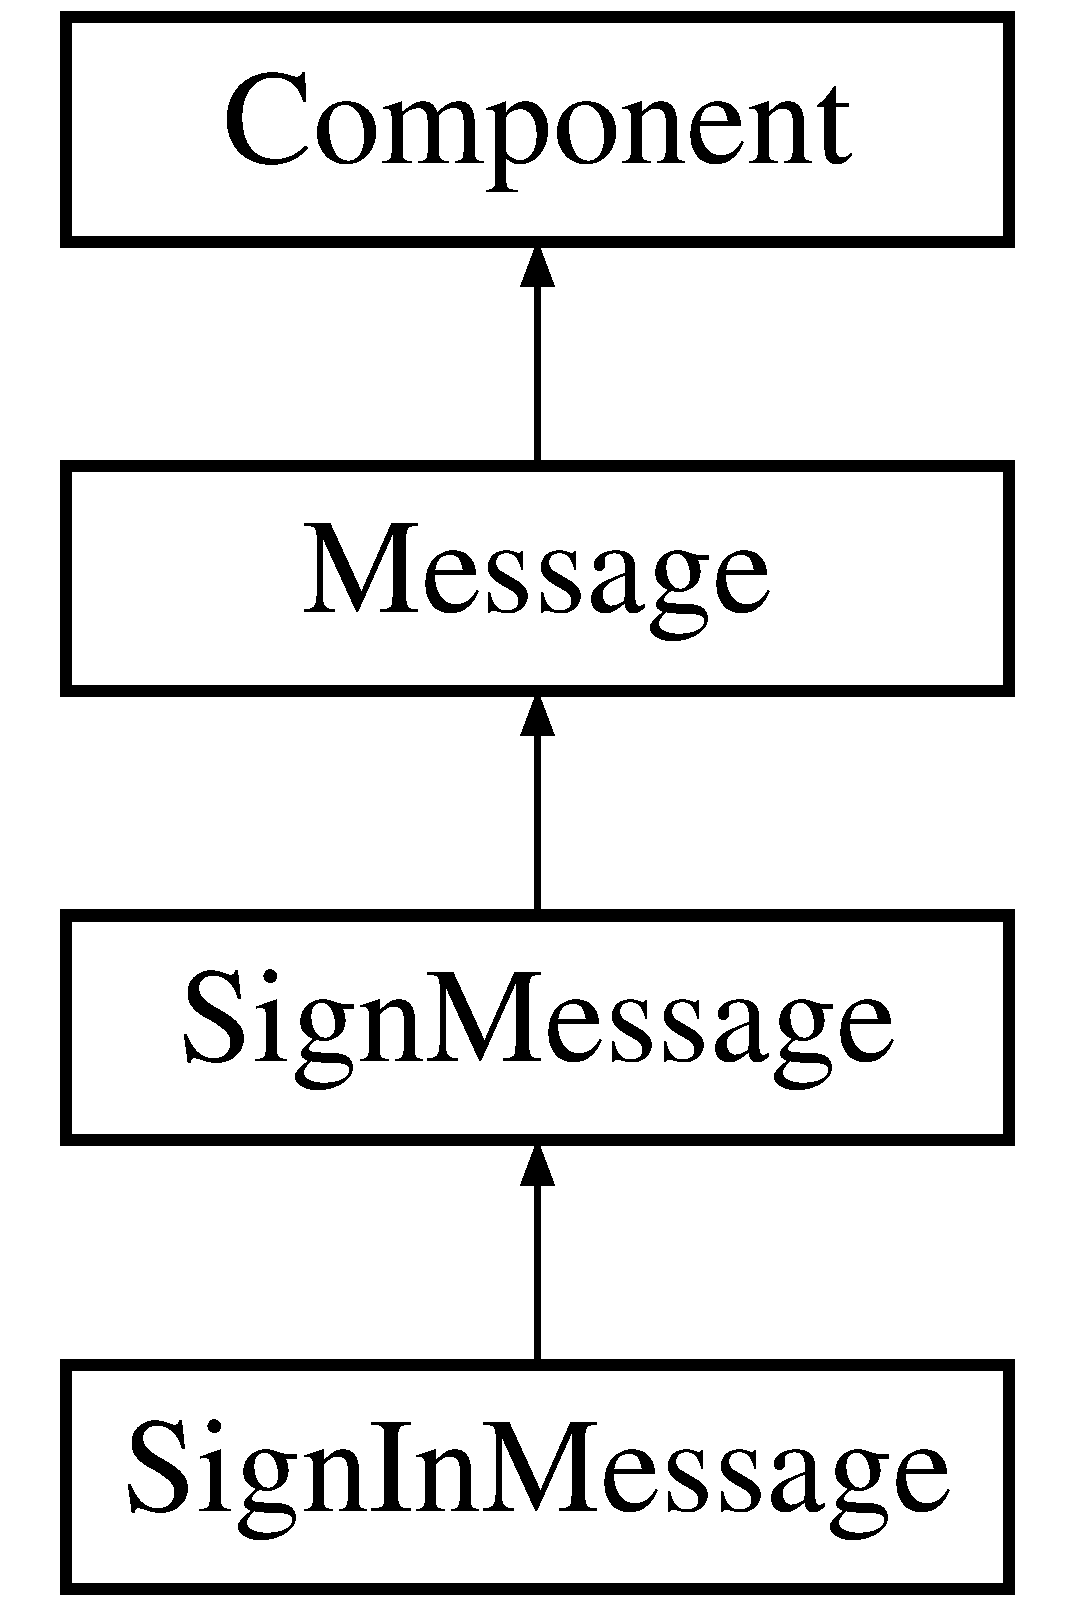
\includegraphics[height=4.000000cm]{classSignInMessage}
\end{center}
\end{figure}
\subsection*{Public Member Functions}
\begin{DoxyCompactItemize}
\item 
\mbox{\Hypertarget{classSignInMessage_accb3dfaad2cca80d6709873a783f895b}\label{classSignInMessage_accb3dfaad2cca80d6709873a783f895b}} 
{\bfseries Sign\+In\+Message} (std\+::string p)
\item 
\mbox{\Hypertarget{classSignMessage_aee897c4bf78df966b8cca95e589566e4}\label{classSignMessage_aee897c4bf78df966b8cca95e589566e4}} 
\mbox{\hyperlink{classElement}{Element}} $\ast$ {\bfseries to\+Element} () const override
\item 
\mbox{\Hypertarget{classMessage_a2a576dcffd45c4574fcdf2897ec26086}\label{classMessage_a2a576dcffd45c4574fcdf2897ec26086}} 
const int {\bfseries get\+\_\+type} () const
\item 
\mbox{\Hypertarget{classComponent_a28212595f8ee85fe009bd233bc99b2fc}\label{classComponent_a28212595f8ee85fe009bd233bc99b2fc}} 
void {\bfseries \+\_\+\+\_\+init\+\_\+\+\_\+} (\mbox{\hyperlink{classElementObject}{Element\+Object}} $\ast$element, const \mbox{\hyperlink{classSerializer}{Serializer}} $\ast$s, const char $\ast$encoding)
\end{DoxyCompactItemize}
\subsection*{Static Public Member Functions}
\begin{DoxyCompactItemize}
\item 
\mbox{\Hypertarget{classMessage_ad92a0e1cfa5b5a503ec9c61833e3e5ea}\label{classMessage_ad92a0e1cfa5b5a503ec9c61833e3e5ea}} 
static \mbox{\hyperlink{classMessage}{Message}} $\ast$ {\bfseries generate} (int id)
\end{DoxyCompactItemize}
\subsection*{Static Public Attributes}
\begin{DoxyCompactItemize}
\item 
\mbox{\Hypertarget{classMessage_a18a7a0d3879210c798f3d84c820f03c1}\label{classMessage_a18a7a0d3879210c798f3d84c820f03c1}} 
static const int {\bfseries T\+R\+A\+N\+S\+A\+C\+T\+I\+ON} = 4
\item 
\mbox{\Hypertarget{classMessage_a3d3ef3111518cd65c0b7f5ec6660888a}\label{classMessage_a3d3ef3111518cd65c0b7f5ec6660888a}} 
static const int {\bfseries B\+L\+O\+CK} = 5
\item 
\mbox{\Hypertarget{classMessage_a9810d3cefb1b33e709cb393583a7a877}\label{classMessage_a9810d3cefb1b33e709cb393583a7a877}} 
static const int {\bfseries A\+S\+K\+\_\+\+P\+E\+E\+RS} = 0
\item 
\mbox{\Hypertarget{classMessage_aa33f42e5795c4df01c7437961d512eaa}\label{classMessage_aa33f42e5795c4df01c7437961d512eaa}} 
static const int {\bfseries A\+N\+S\+W\+E\+R\+\_\+\+P\+E\+E\+RS} = 1
\item 
\mbox{\Hypertarget{classMessage_a64b7688dfdd50a6254bf45b51d2118d4}\label{classMessage_a64b7688dfdd50a6254bf45b51d2118d4}} 
static const int {\bfseries S\+I\+G\+N\+\_\+\+IN} = 2
\item 
\mbox{\Hypertarget{classMessage_aba70c352293fee66004d729ccef3ee48}\label{classMessage_aba70c352293fee66004d729ccef3ee48}} 
static const int {\bfseries S\+I\+G\+N\+\_\+\+O\+UT} = 3
\item 
\mbox{\Hypertarget{classMessage_a62ac5b91838e79a11079869015261e14}\label{classMessage_a62ac5b91838e79a11079869015261e14}} 
static const int {\bfseries A\+S\+K\+\_\+\+B\+L\+O\+CK} = 6
\item 
\mbox{\Hypertarget{classMessage_a1580f4a26d125f71e2af1ef6001ac656}\label{classMessage_a1580f4a26d125f71e2af1ef6001ac656}} 
static const int {\bfseries A\+N\+S\+W\+E\+R\+\_\+\+B\+L\+O\+CK} = 7
\end{DoxyCompactItemize}
\subsection*{Protected Member Functions}
\begin{DoxyCompactItemize}
\item 
\mbox{\Hypertarget{classSignMessage_a35855647925ec76036ed4602743ed118}\label{classSignMessage_a35855647925ec76036ed4602743ed118}} 
void {\bfseries from\+Element} (\mbox{\hyperlink{classElementObject}{Element\+Object}} $\ast$, const \mbox{\hyperlink{classSerializer}{Serializer}} $\ast$serializer, const char $\ast$encoding) override
\end{DoxyCompactItemize}
\subsection*{Protected Attributes}
\begin{DoxyCompactItemize}
\item 
\mbox{\Hypertarget{classMessage_afbfb481c98b13d0deba0bac443bebe29}\label{classMessage_afbfb481c98b13d0deba0bac443bebe29}} 
int {\bfseries type}
\end{DoxyCompactItemize}


The documentation for this class was generated from the following files\+:\begin{DoxyCompactItemize}
\item 
block\+\_\+chain/kernel/messages/Sign\+In\+Message.\+h\item 
block\+\_\+chain/kernel/messages/Sign\+In\+Message.\+cpp\end{DoxyCompactItemize}

\hypertarget{classSignInParser}{}\section{Sign\+In\+Parser Class Reference}
\label{classSignInParser}\index{Sign\+In\+Parser@{Sign\+In\+Parser}}
Inheritance diagram for Sign\+In\+Parser\+:\begin{figure}[H]
\begin{center}
\leavevmode
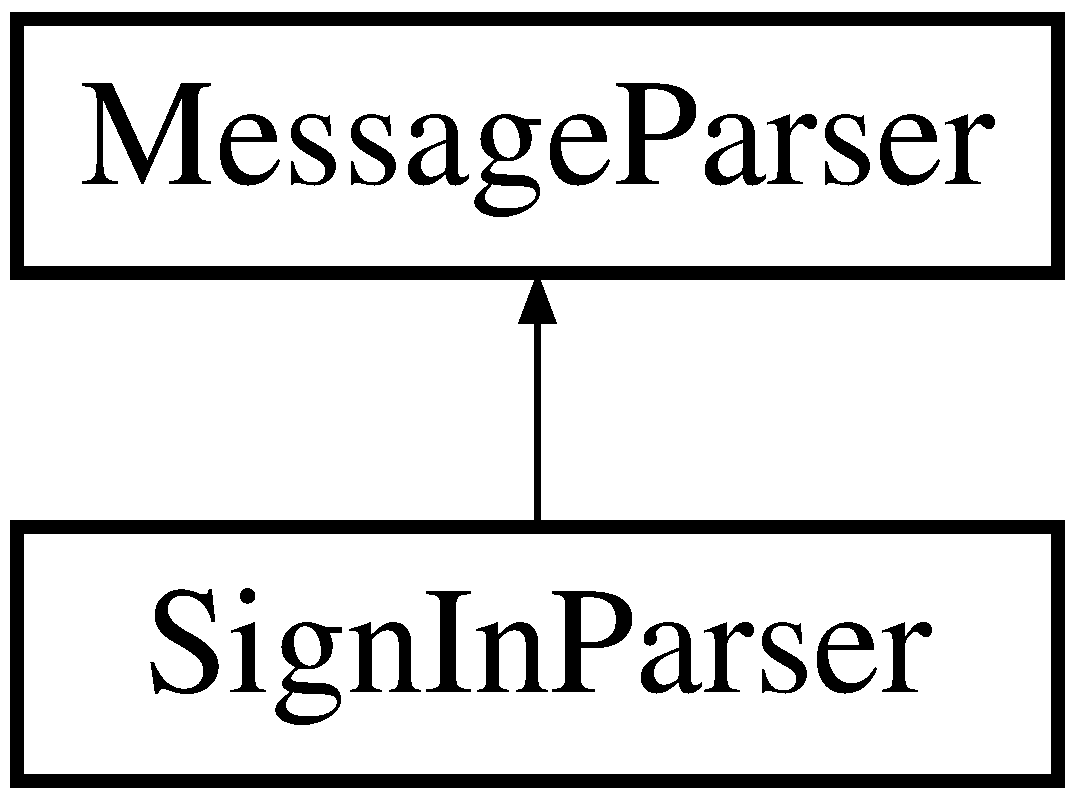
\includegraphics[height=2.000000cm]{classSignInParser}
\end{center}
\end{figure}
\subsection*{Public Member Functions}
\begin{DoxyCompactItemize}
\item 
\mbox{\Hypertarget{classSignInParser_aa73b5113c2c03361469149c456ef9cc0}\label{classSignInParser_aa73b5113c2c03361469149c456ef9cc0}} 
void {\bfseries operator()} (\mbox{\hyperlink{classMessage}{Message}} $\ast$m, \mbox{\hyperlink{classNode}{Node}} $\ast$node) const final
\item 
\mbox{\Hypertarget{classSignInParser_a30af4fa4b99e704e48848aab284d6a24}\label{classSignInParser_a30af4fa4b99e704e48848aab284d6a24}} 
int {\bfseries get\+\_\+type} () const final
\end{DoxyCompactItemize}


The documentation for this class was generated from the following files\+:\begin{DoxyCompactItemize}
\item 
block\+\_\+chain/kernel/parsers/Sign\+In\+Parser.\+h\item 
block\+\_\+chain/kernel/parsers/Sign\+In\+Parser.\+cpp\end{DoxyCompactItemize}

\hypertarget{classSignMessage}{}\section{Sign\+Message Class Reference}
\label{classSignMessage}\index{Sign\+Message@{Sign\+Message}}
Inheritance diagram for Sign\+Message\+:\begin{figure}[H]
\begin{center}
\leavevmode
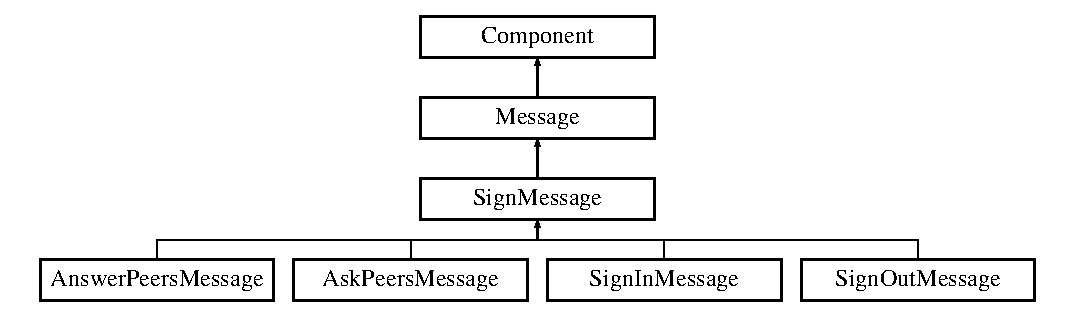
\includegraphics[height=3.809524cm]{classSignMessage}
\end{center}
\end{figure}
\subsection*{Public Member Functions}
\begin{DoxyCompactItemize}
\item 
\mbox{\Hypertarget{classSignMessage_ac1df326e20a41acee483fc8893e791ae}\label{classSignMessage_ac1df326e20a41acee483fc8893e791ae}} 
{\bfseries Sign\+Message} (std\+::string p, int t)
\item 
\mbox{\Hypertarget{classSignMessage_aee897c4bf78df966b8cca95e589566e4}\label{classSignMessage_aee897c4bf78df966b8cca95e589566e4}} 
\mbox{\hyperlink{classElement}{Element}} $\ast$ {\bfseries to\+Element} () const override
\item 
\mbox{\Hypertarget{classMessage_a2a576dcffd45c4574fcdf2897ec26086}\label{classMessage_a2a576dcffd45c4574fcdf2897ec26086}} 
const int {\bfseries get\+\_\+type} () const
\item 
\mbox{\Hypertarget{classComponent_a28212595f8ee85fe009bd233bc99b2fc}\label{classComponent_a28212595f8ee85fe009bd233bc99b2fc}} 
void {\bfseries \+\_\+\+\_\+init\+\_\+\+\_\+} (\mbox{\hyperlink{classElementObject}{Element\+Object}} $\ast$element, const \mbox{\hyperlink{classSerializer}{Serializer}} $\ast$s, const char $\ast$encoding)
\end{DoxyCompactItemize}
\subsection*{Static Public Member Functions}
\begin{DoxyCompactItemize}
\item 
\mbox{\Hypertarget{classMessage_ad92a0e1cfa5b5a503ec9c61833e3e5ea}\label{classMessage_ad92a0e1cfa5b5a503ec9c61833e3e5ea}} 
static \mbox{\hyperlink{classMessage}{Message}} $\ast$ {\bfseries generate} (int id)
\end{DoxyCompactItemize}
\subsection*{Static Public Attributes}
\begin{DoxyCompactItemize}
\item 
\mbox{\Hypertarget{classMessage_a18a7a0d3879210c798f3d84c820f03c1}\label{classMessage_a18a7a0d3879210c798f3d84c820f03c1}} 
static const int {\bfseries T\+R\+A\+N\+S\+A\+C\+T\+I\+ON} = 4
\item 
\mbox{\Hypertarget{classMessage_a3d3ef3111518cd65c0b7f5ec6660888a}\label{classMessage_a3d3ef3111518cd65c0b7f5ec6660888a}} 
static const int {\bfseries B\+L\+O\+CK} = 5
\item 
\mbox{\Hypertarget{classMessage_a9810d3cefb1b33e709cb393583a7a877}\label{classMessage_a9810d3cefb1b33e709cb393583a7a877}} 
static const int {\bfseries A\+S\+K\+\_\+\+P\+E\+E\+RS} = 0
\item 
\mbox{\Hypertarget{classMessage_aa33f42e5795c4df01c7437961d512eaa}\label{classMessage_aa33f42e5795c4df01c7437961d512eaa}} 
static const int {\bfseries A\+N\+S\+W\+E\+R\+\_\+\+P\+E\+E\+RS} = 1
\item 
\mbox{\Hypertarget{classMessage_a64b7688dfdd50a6254bf45b51d2118d4}\label{classMessage_a64b7688dfdd50a6254bf45b51d2118d4}} 
static const int {\bfseries S\+I\+G\+N\+\_\+\+IN} = 2
\item 
\mbox{\Hypertarget{classMessage_aba70c352293fee66004d729ccef3ee48}\label{classMessage_aba70c352293fee66004d729ccef3ee48}} 
static const int {\bfseries S\+I\+G\+N\+\_\+\+O\+UT} = 3
\item 
\mbox{\Hypertarget{classMessage_a62ac5b91838e79a11079869015261e14}\label{classMessage_a62ac5b91838e79a11079869015261e14}} 
static const int {\bfseries A\+S\+K\+\_\+\+B\+L\+O\+CK} = 6
\item 
\mbox{\Hypertarget{classMessage_a1580f4a26d125f71e2af1ef6001ac656}\label{classMessage_a1580f4a26d125f71e2af1ef6001ac656}} 
static const int {\bfseries A\+N\+S\+W\+E\+R\+\_\+\+B\+L\+O\+CK} = 7
\end{DoxyCompactItemize}
\subsection*{Protected Member Functions}
\begin{DoxyCompactItemize}
\item 
\mbox{\Hypertarget{classSignMessage_a35855647925ec76036ed4602743ed118}\label{classSignMessage_a35855647925ec76036ed4602743ed118}} 
void {\bfseries from\+Element} (\mbox{\hyperlink{classElementObject}{Element\+Object}} $\ast$, const \mbox{\hyperlink{classSerializer}{Serializer}} $\ast$serializer, const char $\ast$encoding) override
\end{DoxyCompactItemize}
\subsection*{Protected Attributes}
\begin{DoxyCompactItemize}
\item 
\mbox{\Hypertarget{classMessage_afbfb481c98b13d0deba0bac443bebe29}\label{classMessage_afbfb481c98b13d0deba0bac443bebe29}} 
int {\bfseries type}
\end{DoxyCompactItemize}
\subsection*{Friends}
\begin{DoxyCompactItemize}
\item 
\mbox{\Hypertarget{classSignMessage_aedbc6d52e9be9e8e9b9e185d53352518}\label{classSignMessage_aedbc6d52e9be9e8e9b9e185d53352518}} 
class {\bfseries Sign\+In\+Parser}
\item 
\mbox{\Hypertarget{classSignMessage_ad8b6311fd20b52f64b7ab8838b5c74d1}\label{classSignMessage_ad8b6311fd20b52f64b7ab8838b5c74d1}} 
class {\bfseries Sign\+Out\+Parser}
\item 
\mbox{\Hypertarget{classSignMessage_a4e698afe7d3c1a9bbb147968cd3d0967}\label{classSignMessage_a4e698afe7d3c1a9bbb147968cd3d0967}} 
class {\bfseries Peers\+Ask\+Parser}
\item 
\mbox{\Hypertarget{classSignMessage_a9e3cdec4aeecdf3e8af4ce55247056b5}\label{classSignMessage_a9e3cdec4aeecdf3e8af4ce55247056b5}} 
class {\bfseries Peers\+Answer\+Parser}
\end{DoxyCompactItemize}


The documentation for this class was generated from the following files\+:\begin{DoxyCompactItemize}
\item 
block\+\_\+chain/kernel/messages/Sign\+Message.\+h\item 
block\+\_\+chain/kernel/messages/Sign\+Message.\+cpp\end{DoxyCompactItemize}

\hypertarget{classSignOutMessage}{}\section{Sign\+Out\+Message Class Reference}
\label{classSignOutMessage}\index{Sign\+Out\+Message@{Sign\+Out\+Message}}
Inheritance diagram for Sign\+Out\+Message\+:\begin{figure}[H]
\begin{center}
\leavevmode
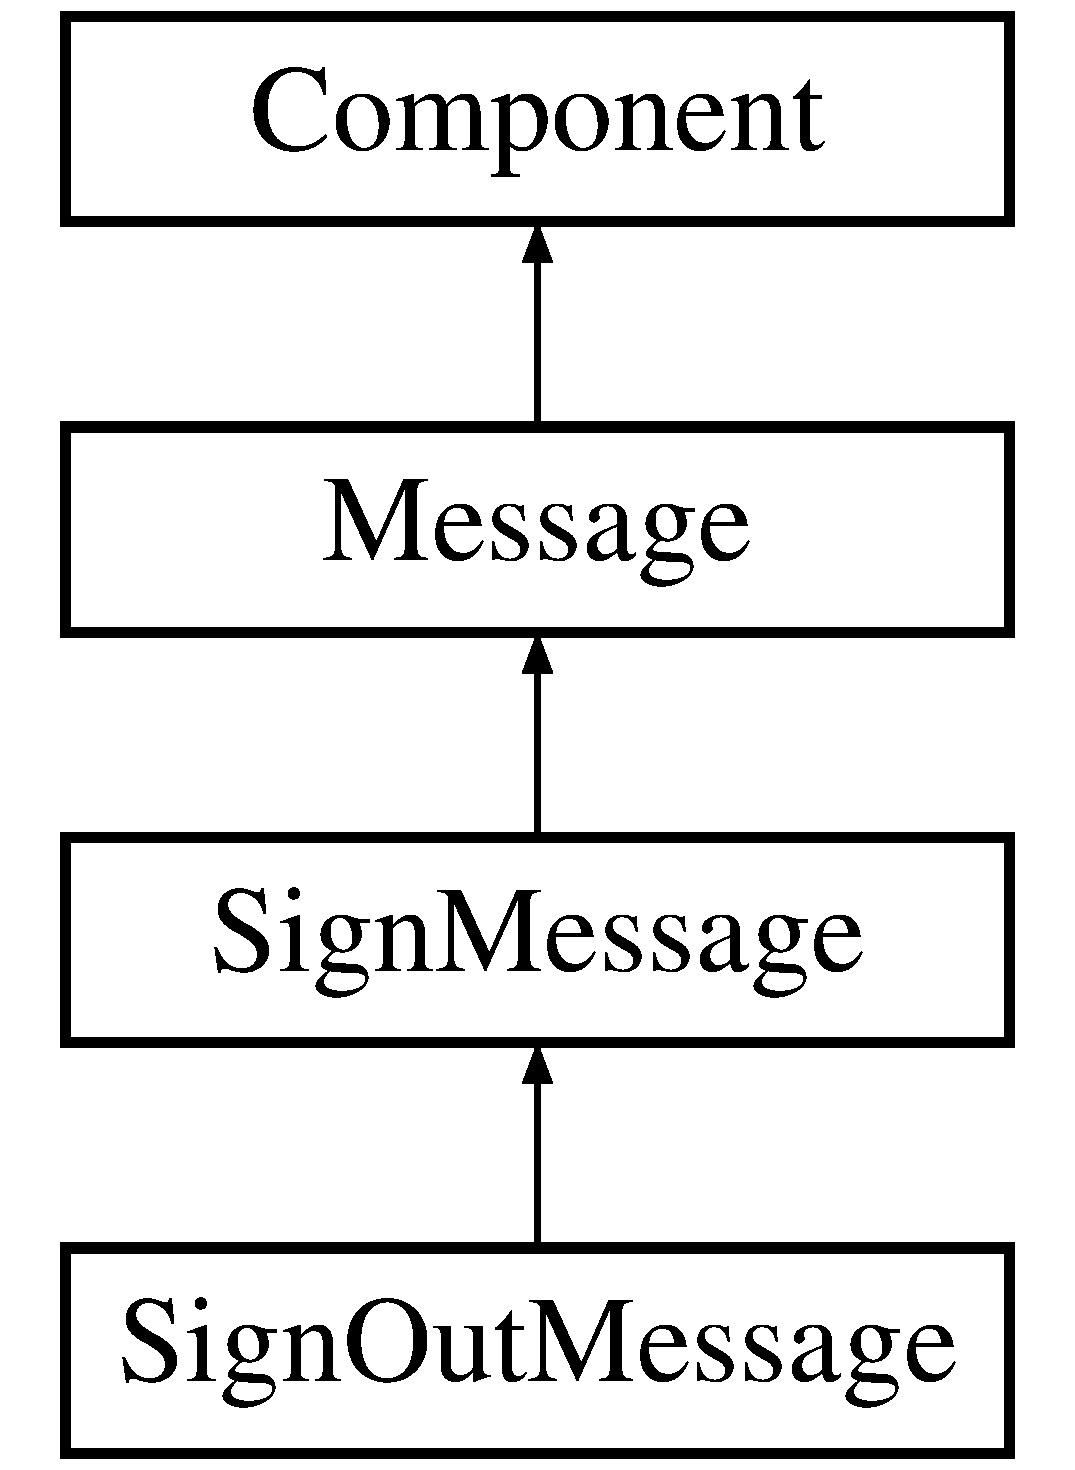
\includegraphics[height=4.000000cm]{classSignOutMessage}
\end{center}
\end{figure}
\subsection*{Public Member Functions}
\begin{DoxyCompactItemize}
\item 
\mbox{\Hypertarget{classSignOutMessage_afbc16960cf71f0259ed990e88cf19f38}\label{classSignOutMessage_afbc16960cf71f0259ed990e88cf19f38}} 
{\bfseries Sign\+Out\+Message} (std\+::string p)
\item 
\mbox{\Hypertarget{classSignMessage_aee897c4bf78df966b8cca95e589566e4}\label{classSignMessage_aee897c4bf78df966b8cca95e589566e4}} 
\mbox{\hyperlink{classElement}{Element}} $\ast$ {\bfseries to\+Element} () const override
\item 
\mbox{\Hypertarget{classMessage_a2a576dcffd45c4574fcdf2897ec26086}\label{classMessage_a2a576dcffd45c4574fcdf2897ec26086}} 
const int {\bfseries get\+\_\+type} () const
\item 
\mbox{\Hypertarget{classComponent_a28212595f8ee85fe009bd233bc99b2fc}\label{classComponent_a28212595f8ee85fe009bd233bc99b2fc}} 
void {\bfseries \+\_\+\+\_\+init\+\_\+\+\_\+} (\mbox{\hyperlink{classElementObject}{Element\+Object}} $\ast$element, const \mbox{\hyperlink{classSerializer}{Serializer}} $\ast$s, const char $\ast$encoding)
\end{DoxyCompactItemize}
\subsection*{Static Public Member Functions}
\begin{DoxyCompactItemize}
\item 
\mbox{\Hypertarget{classMessage_ad92a0e1cfa5b5a503ec9c61833e3e5ea}\label{classMessage_ad92a0e1cfa5b5a503ec9c61833e3e5ea}} 
static \mbox{\hyperlink{classMessage}{Message}} $\ast$ {\bfseries generate} (int id)
\end{DoxyCompactItemize}
\subsection*{Static Public Attributes}
\begin{DoxyCompactItemize}
\item 
\mbox{\Hypertarget{classMessage_a18a7a0d3879210c798f3d84c820f03c1}\label{classMessage_a18a7a0d3879210c798f3d84c820f03c1}} 
static const int {\bfseries T\+R\+A\+N\+S\+A\+C\+T\+I\+ON} = 4
\item 
\mbox{\Hypertarget{classMessage_a3d3ef3111518cd65c0b7f5ec6660888a}\label{classMessage_a3d3ef3111518cd65c0b7f5ec6660888a}} 
static const int {\bfseries B\+L\+O\+CK} = 5
\item 
\mbox{\Hypertarget{classMessage_a9810d3cefb1b33e709cb393583a7a877}\label{classMessage_a9810d3cefb1b33e709cb393583a7a877}} 
static const int {\bfseries A\+S\+K\+\_\+\+P\+E\+E\+RS} = 0
\item 
\mbox{\Hypertarget{classMessage_aa33f42e5795c4df01c7437961d512eaa}\label{classMessage_aa33f42e5795c4df01c7437961d512eaa}} 
static const int {\bfseries A\+N\+S\+W\+E\+R\+\_\+\+P\+E\+E\+RS} = 1
\item 
\mbox{\Hypertarget{classMessage_a64b7688dfdd50a6254bf45b51d2118d4}\label{classMessage_a64b7688dfdd50a6254bf45b51d2118d4}} 
static const int {\bfseries S\+I\+G\+N\+\_\+\+IN} = 2
\item 
\mbox{\Hypertarget{classMessage_aba70c352293fee66004d729ccef3ee48}\label{classMessage_aba70c352293fee66004d729ccef3ee48}} 
static const int {\bfseries S\+I\+G\+N\+\_\+\+O\+UT} = 3
\item 
\mbox{\Hypertarget{classMessage_a62ac5b91838e79a11079869015261e14}\label{classMessage_a62ac5b91838e79a11079869015261e14}} 
static const int {\bfseries A\+S\+K\+\_\+\+B\+L\+O\+CK} = 6
\item 
\mbox{\Hypertarget{classMessage_a1580f4a26d125f71e2af1ef6001ac656}\label{classMessage_a1580f4a26d125f71e2af1ef6001ac656}} 
static const int {\bfseries A\+N\+S\+W\+E\+R\+\_\+\+B\+L\+O\+CK} = 7
\end{DoxyCompactItemize}
\subsection*{Protected Member Functions}
\begin{DoxyCompactItemize}
\item 
\mbox{\Hypertarget{classSignMessage_a35855647925ec76036ed4602743ed118}\label{classSignMessage_a35855647925ec76036ed4602743ed118}} 
void {\bfseries from\+Element} (\mbox{\hyperlink{classElementObject}{Element\+Object}} $\ast$, const \mbox{\hyperlink{classSerializer}{Serializer}} $\ast$serializer, const char $\ast$encoding) override
\end{DoxyCompactItemize}
\subsection*{Protected Attributes}
\begin{DoxyCompactItemize}
\item 
\mbox{\Hypertarget{classMessage_afbfb481c98b13d0deba0bac443bebe29}\label{classMessage_afbfb481c98b13d0deba0bac443bebe29}} 
int {\bfseries type}
\end{DoxyCompactItemize}


The documentation for this class was generated from the following files\+:\begin{DoxyCompactItemize}
\item 
block\+\_\+chain/kernel/messages/Sign\+Out\+Message.\+h\item 
block\+\_\+chain/kernel/messages/Sign\+Out\+Message.\+cpp\end{DoxyCompactItemize}

\hypertarget{classSignOutParser}{}\section{Sign\+Out\+Parser Class Reference}
\label{classSignOutParser}\index{Sign\+Out\+Parser@{Sign\+Out\+Parser}}
Inheritance diagram for Sign\+Out\+Parser\+:\begin{figure}[H]
\begin{center}
\leavevmode
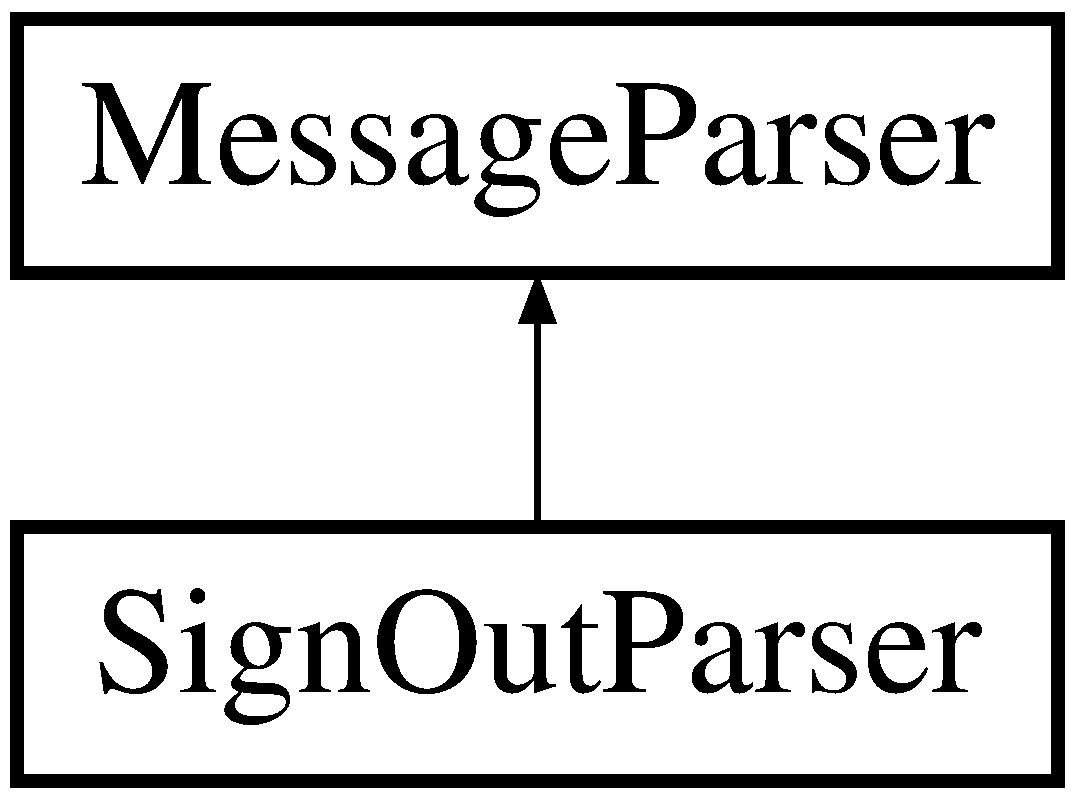
\includegraphics[height=2.000000cm]{classSignOutParser}
\end{center}
\end{figure}
\subsection*{Public Member Functions}
\begin{DoxyCompactItemize}
\item 
\mbox{\Hypertarget{classSignOutParser_a29ec80b982d783c10d46a431947bb319}\label{classSignOutParser_a29ec80b982d783c10d46a431947bb319}} 
void {\bfseries operator()} (\mbox{\hyperlink{classMessage}{Message}} $\ast$m, \mbox{\hyperlink{classNode}{Node}} $\ast$node) const final
\item 
\mbox{\Hypertarget{classSignOutParser_afe949de785ce36746d69e19515a72d24}\label{classSignOutParser_afe949de785ce36746d69e19515a72d24}} 
int {\bfseries get\+\_\+type} () const final
\end{DoxyCompactItemize}


The documentation for this class was generated from the following files\+:\begin{DoxyCompactItemize}
\item 
block\+\_\+chain/kernel/parsers/Sign\+Out\+Parser.\+h\item 
block\+\_\+chain/kernel/parsers/Sign\+Out\+Parser.\+cpp\end{DoxyCompactItemize}

\hypertarget{classSocket}{}\section{Socket Class Reference}
\label{classSocket}\index{Socket@{Socket}}


{\ttfamily \#include $<$Socket.\+h$>$}

\subsection*{Public Member Functions}
\begin{DoxyCompactItemize}
\item 
\mbox{\hyperlink{classSocket_a4c7a40e6c1513edf63e53b74b4f32b80}{Socket}} (std\+::string i, int port)
\item 
\mbox{\hyperlink{classSocket_a7e2193bd6a9b6846f90eaf4786cfc41b}{Socket}} (S\+O\+C\+K\+ET s)
\item 
void \mbox{\hyperlink{classSocket_ab7c6b44800e7a621df9edae86d5fdfa8}{\+\_\+bind}} (sockaddr\+\_\+in $\ast$sin)
\item 
void \mbox{\hyperlink{classSocket_ac54a69178584b414d8137170156ad742}{\+\_\+listen}} ()
\item 
void \mbox{\hyperlink{classSocket_a284f2130a4115a77ebce742427fd0bdb}{\+\_\+close}} ()
\item 
int \mbox{\hyperlink{classSocket_a74fc13f1e87009d84871d73949a664b2}{read}} (std\+::string \&buffer)
\item 
int \mbox{\hyperlink{classSocket_ae2f8cf0b7d27c59600dc5ddf65f8a884}{write}} (const char $\ast$buffer)
\item 
\mbox{\hyperlink{classSocket}{Socket}} $\ast$ \mbox{\hyperlink{classSocket_a153f0c90d33f1d60133b3ab565679013}{\+\_\+accept}} (sockaddr\+\_\+in $\ast$csin, accept\+\_\+size size)
\item 
\mbox{\hyperlink{classSocket_aeac4eb6379a543d38ed88977d3b6630a}{$\sim$\+Socket}} ()
\end{DoxyCompactItemize}
\subsection*{Static Public Member Functions}
\begin{DoxyCompactItemize}
\item 
static std\+::string \mbox{\hyperlink{classSocket_a5f78c7dbb42b062df843a66431acd0de}{get\+IP}} ()
\end{DoxyCompactItemize}


\subsection{Detailed Description}
The class that listen to the port

\begin{DoxyAuthor}{Author}
Mathieu Lochet 
\end{DoxyAuthor}
\begin{DoxyVersion}{Version}
3 
\end{DoxyVersion}


\subsection{Constructor \& Destructor Documentation}
\mbox{\Hypertarget{classSocket_a4c7a40e6c1513edf63e53b74b4f32b80}\label{classSocket_a4c7a40e6c1513edf63e53b74b4f32b80}} 
\index{Socket@{Socket}!Socket@{Socket}}
\index{Socket@{Socket}!Socket@{Socket}}
\subsubsection{\texorpdfstring{Socket()}{Socket()}\hspace{0.1cm}{\footnotesize\ttfamily [1/2]}}
{\footnotesize\ttfamily Socket\+::\+Socket (\begin{DoxyParamCaption}\item[{std\+::string}]{i,  }\item[{int}]{port }\end{DoxyParamCaption})}

The constructor that generates a socket with a given IP and port


\begin{DoxyParams}{Parameters}
{\em i} & the IP to connect to \\
\hline
{\em port} & the port the connect to \\
\hline
\end{DoxyParams}
\mbox{\Hypertarget{classSocket_a7e2193bd6a9b6846f90eaf4786cfc41b}\label{classSocket_a7e2193bd6a9b6846f90eaf4786cfc41b}} 
\index{Socket@{Socket}!Socket@{Socket}}
\index{Socket@{Socket}!Socket@{Socket}}
\subsubsection{\texorpdfstring{Socket()}{Socket()}\hspace{0.1cm}{\footnotesize\ttfamily [2/2]}}
{\footnotesize\ttfamily Socket\+::\+Socket (\begin{DoxyParamCaption}\item[{S\+O\+C\+K\+ET}]{s }\end{DoxyParamCaption})\hspace{0.3cm}{\ttfamily [explicit]}}

The constructor that generates a socket with a S\+O\+C\+K\+ET value


\begin{DoxyParams}{Parameters}
{\em s} & the S\+O\+C\+K\+ET value \\
\hline
\end{DoxyParams}
\mbox{\Hypertarget{classSocket_aeac4eb6379a543d38ed88977d3b6630a}\label{classSocket_aeac4eb6379a543d38ed88977d3b6630a}} 
\index{Socket@{Socket}!````~Socket@{$\sim$\+Socket}}
\index{````~Socket@{$\sim$\+Socket}!Socket@{Socket}}
\subsubsection{\texorpdfstring{$\sim$\+Socket()}{~Socket()}}
{\footnotesize\ttfamily Socket\+::$\sim$\+Socket (\begin{DoxyParamCaption}{ }\end{DoxyParamCaption})}

Close the socket connection 

\subsection{Member Function Documentation}
\mbox{\Hypertarget{classSocket_a153f0c90d33f1d60133b3ab565679013}\label{classSocket_a153f0c90d33f1d60133b3ab565679013}} 
\index{Socket@{Socket}!\+\_\+accept@{\+\_\+accept}}
\index{\+\_\+accept@{\+\_\+accept}!Socket@{Socket}}
\subsubsection{\texorpdfstring{\+\_\+accept()}{\_accept()}}
{\footnotesize\ttfamily \mbox{\hyperlink{classSocket}{Socket}} $\ast$ Socket\+::\+\_\+accept (\begin{DoxyParamCaption}\item[{sockaddr\+\_\+in $\ast$}]{csin,  }\item[{accept\+\_\+size}]{size }\end{DoxyParamCaption})}

Wait and accepts a connection on the server


\begin{DoxyParams}{Parameters}
{\em csin} & a socket address \\
\hline
{\em size} & the size of the socket address \\
\hline
\end{DoxyParams}
\begin{DoxyReturn}{Returns}
1 if success, 0 if failure 
\end{DoxyReturn}
\mbox{\Hypertarget{classSocket_ab7c6b44800e7a621df9edae86d5fdfa8}\label{classSocket_ab7c6b44800e7a621df9edae86d5fdfa8}} 
\index{Socket@{Socket}!\+\_\+bind@{\+\_\+bind}}
\index{\+\_\+bind@{\+\_\+bind}!Socket@{Socket}}
\subsubsection{\texorpdfstring{\+\_\+bind()}{\_bind()}}
{\footnotesize\ttfamily void Socket\+::\+\_\+bind (\begin{DoxyParamCaption}\item[{sockaddr\+\_\+in $\ast$}]{sin }\end{DoxyParamCaption})}

Bind the socket to a given address so it can listen to connections


\begin{DoxyParams}{Parameters}
{\em sin} & the given address \\
\hline
\end{DoxyParams}
\mbox{\Hypertarget{classSocket_a284f2130a4115a77ebce742427fd0bdb}\label{classSocket_a284f2130a4115a77ebce742427fd0bdb}} 
\index{Socket@{Socket}!\+\_\+close@{\+\_\+close}}
\index{\+\_\+close@{\+\_\+close}!Socket@{Socket}}
\subsubsection{\texorpdfstring{\+\_\+close()}{\_close()}}
{\footnotesize\ttfamily void Socket\+::\+\_\+close (\begin{DoxyParamCaption}{ }\end{DoxyParamCaption})}

Close the socket connection \mbox{\Hypertarget{classSocket_ac54a69178584b414d8137170156ad742}\label{classSocket_ac54a69178584b414d8137170156ad742}} 
\index{Socket@{Socket}!\+\_\+listen@{\+\_\+listen}}
\index{\+\_\+listen@{\+\_\+listen}!Socket@{Socket}}
\subsubsection{\texorpdfstring{\+\_\+listen()}{\_listen()}}
{\footnotesize\ttfamily void Socket\+::\+\_\+listen (\begin{DoxyParamCaption}{ }\end{DoxyParamCaption})}

Listen to connections \mbox{\Hypertarget{classSocket_a5f78c7dbb42b062df843a66431acd0de}\label{classSocket_a5f78c7dbb42b062df843a66431acd0de}} 
\index{Socket@{Socket}!get\+IP@{get\+IP}}
\index{get\+IP@{get\+IP}!Socket@{Socket}}
\subsubsection{\texorpdfstring{get\+I\+P()}{getIP()}}
{\footnotesize\ttfamily std\+::string Socket\+::get\+IP (\begin{DoxyParamCaption}{ }\end{DoxyParamCaption})\hspace{0.3cm}{\ttfamily [static]}}

Generate the IP of the computer

\begin{DoxyReturn}{Returns}
The IP of the computer 
\end{DoxyReturn}
\mbox{\Hypertarget{classSocket_a74fc13f1e87009d84871d73949a664b2}\label{classSocket_a74fc13f1e87009d84871d73949a664b2}} 
\index{Socket@{Socket}!read@{read}}
\index{read@{read}!Socket@{Socket}}
\subsubsection{\texorpdfstring{read()}{read()}}
{\footnotesize\ttfamily int Socket\+::read (\begin{DoxyParamCaption}\item[{std\+::string \&}]{buffer }\end{DoxyParamCaption})}

Read values from the socket when a packet in received


\begin{DoxyParams}{Parameters}
{\em buffer} & the buffer in which to write the packet \\
\hline
\end{DoxyParams}
\begin{DoxyReturn}{Returns}
1 if success, 0 if failure 
\end{DoxyReturn}
\mbox{\Hypertarget{classSocket_ae2f8cf0b7d27c59600dc5ddf65f8a884}\label{classSocket_ae2f8cf0b7d27c59600dc5ddf65f8a884}} 
\index{Socket@{Socket}!write@{write}}
\index{write@{write}!Socket@{Socket}}
\subsubsection{\texorpdfstring{write()}{write()}}
{\footnotesize\ttfamily int Socket\+::write (\begin{DoxyParamCaption}\item[{const char $\ast$}]{buffer }\end{DoxyParamCaption})}

Write a packet to a given packet


\begin{DoxyParams}{Parameters}
{\em buffer} & the buffer to send to the peer \\
\hline
\end{DoxyParams}
\begin{DoxyReturn}{Returns}
1 if success, 0 if failure 
\end{DoxyReturn}


The documentation for this class was generated from the following files\+:\begin{DoxyCompactItemize}
\item 
block\+\_\+chain/utils/socket/Socket.\+h\item 
block\+\_\+chain/utils/socket/Socket.\+cpp\end{DoxyCompactItemize}

\hypertarget{classSocketServer}{}\section{Socket\+Server Class Reference}
\label{classSocketServer}\index{Socket\+Server@{Socket\+Server}}


{\ttfamily \#include $<$Socket\+Server.\+h$>$}

\subsection*{Public Member Functions}
\begin{DoxyCompactItemize}
\item 
\mbox{\hyperlink{classSocketServer_a73939197c857f63eede6fc2f0c6ab433}{Socket\+Server}} (int port)
\item 
void \mbox{\hyperlink{classSocketServer_aba550d54be7cb671b850085280b29506}{run}} (std\+::function$<$ bool(\mbox{\hyperlink{classSocket}{Socket}} $\ast$, int, \mbox{\hyperlink{classSerializer}{Serializer}} $\ast$serializer, \mbox{\hyperlink{classNode}{Node}} $\ast$node)$>$ func, \mbox{\hyperlink{classSerializer}{Serializer}} $\ast$serializer, \mbox{\hyperlink{classNode}{Node}} $\ast$node)
\item 
void \mbox{\hyperlink{classSocketServer_aaaa3c5145b286c3d492f9bf1bec5a5dc}{run}} (\mbox{\hyperlink{classSerializer}{Serializer}} $\ast$serializer, \mbox{\hyperlink{classNode}{Node}} $\ast$node)
\item 
\mbox{\hyperlink{classSocketServer_af0e595690e453ef4b8e8da174069aba9}{$\sim$\+Socket\+Server}} ()
\item 
void \mbox{\hyperlink{classSocketServer_a1e673e526a459bdb3ca92e103ec212ae}{close}} ()
\end{DoxyCompactItemize}


\subsection{Detailed Description}
The class that listen to the port

\begin{DoxyAuthor}{Author}
Mathieu Lochet 
\end{DoxyAuthor}
\begin{DoxyVersion}{Version}
3 
\end{DoxyVersion}


\subsection{Constructor \& Destructor Documentation}
\mbox{\Hypertarget{classSocketServer_a73939197c857f63eede6fc2f0c6ab433}\label{classSocketServer_a73939197c857f63eede6fc2f0c6ab433}} 
\index{Socket\+Server@{Socket\+Server}!Socket\+Server@{Socket\+Server}}
\index{Socket\+Server@{Socket\+Server}!Socket\+Server@{Socket\+Server}}
\subsubsection{\texorpdfstring{Socket\+Server()}{SocketServer()}}
{\footnotesize\ttfamily Socket\+Server\+::\+Socket\+Server (\begin{DoxyParamCaption}\item[{int}]{port }\end{DoxyParamCaption})\hspace{0.3cm}{\ttfamily [explicit]}}

The constructor that generates the connection on the given port \begin{DoxySeeAlso}{See also}
\mbox{\hyperlink{classSocket}{Socket}}
\end{DoxySeeAlso}

\begin{DoxyParams}{Parameters}
{\em port} & the port the listen to \\
\hline
\end{DoxyParams}
\mbox{\Hypertarget{classSocketServer_af0e595690e453ef4b8e8da174069aba9}\label{classSocketServer_af0e595690e453ef4b8e8da174069aba9}} 
\index{Socket\+Server@{Socket\+Server}!````~Socket\+Server@{$\sim$\+Socket\+Server}}
\index{````~Socket\+Server@{$\sim$\+Socket\+Server}!Socket\+Server@{Socket\+Server}}
\subsubsection{\texorpdfstring{$\sim$\+Socket\+Server()}{~SocketServer()}}
{\footnotesize\ttfamily Socket\+Server\+::$\sim$\+Socket\+Server (\begin{DoxyParamCaption}{ }\end{DoxyParamCaption})}

The destructor closes the connection with the other peers 

\subsection{Member Function Documentation}
\mbox{\Hypertarget{classSocketServer_a1e673e526a459bdb3ca92e103ec212ae}\label{classSocketServer_a1e673e526a459bdb3ca92e103ec212ae}} 
\index{Socket\+Server@{Socket\+Server}!close@{close}}
\index{close@{close}!Socket\+Server@{Socket\+Server}}
\subsubsection{\texorpdfstring{close()}{close()}}
{\footnotesize\ttfamily void Socket\+Server\+::close (\begin{DoxyParamCaption}{ }\end{DoxyParamCaption})}

Closes the connection with the other peers \mbox{\Hypertarget{classSocketServer_aba550d54be7cb671b850085280b29506}\label{classSocketServer_aba550d54be7cb671b850085280b29506}} 
\index{Socket\+Server@{Socket\+Server}!run@{run}}
\index{run@{run}!Socket\+Server@{Socket\+Server}}
\subsubsection{\texorpdfstring{run()}{run()}\hspace{0.1cm}{\footnotesize\ttfamily [1/2]}}
{\footnotesize\ttfamily void Socket\+Server\+::run (\begin{DoxyParamCaption}\item[{std\+::function$<$ bool(\mbox{\hyperlink{classSocket}{Socket}} $\ast$, int, \mbox{\hyperlink{classSerializer}{Serializer}} $\ast$serializer, \mbox{\hyperlink{classNode}{Node}} $\ast$node)$>$}]{func,  }\item[{\mbox{\hyperlink{classSerializer}{Serializer}} $\ast$}]{serializer,  }\item[{\mbox{\hyperlink{classNode}{Node}} $\ast$}]{node }\end{DoxyParamCaption})}

Run the server with a given callback \begin{DoxySeeAlso}{See also}
\mbox{\hyperlink{classSocket}{Socket}} 

\mbox{\hyperlink{classSerializer}{Serializer}} 

\mbox{\hyperlink{classNode}{Node}}
\end{DoxySeeAlso}

\begin{DoxyParams}{Parameters}
{\em func} & the callback to use with each client. The callback must have a prototype such as \char`\"{}bool (\+Socket$\ast$, Serializer$\ast$, Node$\ast$)\char`\"{} \\
\hline
{\em serializer} & the serializer to use to parse packets \\
\hline
{\em node} & the client that uses the server \\
\hline
\end{DoxyParams}
\mbox{\Hypertarget{classSocketServer_aaaa3c5145b286c3d492f9bf1bec5a5dc}\label{classSocketServer_aaaa3c5145b286c3d492f9bf1bec5a5dc}} 
\index{Socket\+Server@{Socket\+Server}!run@{run}}
\index{run@{run}!Socket\+Server@{Socket\+Server}}
\subsubsection{\texorpdfstring{run()}{run()}\hspace{0.1cm}{\footnotesize\ttfamily [2/2]}}
{\footnotesize\ttfamily void Socket\+Server\+::run (\begin{DoxyParamCaption}\item[{\mbox{\hyperlink{classSerializer}{Serializer}} $\ast$}]{serializer,  }\item[{\mbox{\hyperlink{classNode}{Node}} $\ast$}]{node }\end{DoxyParamCaption})}

Run the server with a default callback \begin{DoxyRefDesc}{Deprecated}
\item[\mbox{\hyperlink{deprecated__deprecated000001}{Deprecated}}]\end{DoxyRefDesc}
\begin{DoxySeeAlso}{See also}
\mbox{\hyperlink{classSerializer}{Serializer}} 

\mbox{\hyperlink{classNode}{Node}}
\end{DoxySeeAlso}

\begin{DoxyParams}{Parameters}
{\em serializer} & the serializer to use to parse packets \\
\hline
{\em node} & the client that uses the server \\
\hline
\end{DoxyParams}


The documentation for this class was generated from the following files\+:\begin{DoxyCompactItemize}
\item 
block\+\_\+chain/utils/socket/Socket\+Server.\+h\item 
block\+\_\+chain/utils/socket/Socket\+Server.\+cpp\end{DoxyCompactItemize}

\hypertarget{classStatusTransaction}{}\section{Status\+Transaction Class Reference}
\label{classStatusTransaction}\index{Status\+Transaction@{Status\+Transaction}}
Inheritance diagram for Status\+Transaction\+:\begin{figure}[H]
\begin{center}
\leavevmode
\includegraphics[height=3.000000cm]{classStatusTransaction}
\end{center}
\end{figure}
\subsection*{Public Member Functions}
\begin{DoxyCompactItemize}
\item 
\mbox{\Hypertarget{classStatusTransaction_a29621e2caa076e885fd533d32b305dbc}\label{classStatusTransaction_a29621e2caa076e885fd533d32b305dbc}} 
bool {\bfseries operator()} () const final
\item 
\mbox{\Hypertarget{classStatusTransaction_aed42f2d61f2d50ec07bb6b35473f61f2}\label{classStatusTransaction_aed42f2d61f2d50ec07bb6b35473f61f2}} 
\mbox{\hyperlink{classElement}{Element}} $\ast$ {\bfseries to\+Element} () const override
\item 
\mbox{\Hypertarget{classStatusTransaction_a4d4c3a2be0d52e7f54675033cdf66881}\label{classStatusTransaction_a4d4c3a2be0d52e7f54675033cdf66881}} 
bool {\bfseries operator==} (\mbox{\hyperlink{classTransaction}{Transaction}} $\ast$t) const override
\item 
\mbox{\Hypertarget{classStatusTransaction_a184e95e0177fdb8e55f7b9100dcda1c7}\label{classStatusTransaction_a184e95e0177fdb8e55f7b9100dcda1c7}} 
std\+::string {\bfseries to\+\_\+string} () const
\item 
\mbox{\Hypertarget{classStatusTransaction_a77d1d73cf3faa9d9e10753420536377a}\label{classStatusTransaction_a77d1d73cf3faa9d9e10753420536377a}} 
std\+::vector$<$ std\+::string $>$ {\bfseries apply} (\mbox{\hyperlink{classRow}{Row}} $\ast$row) override
\item 
\mbox{\Hypertarget{classStatusTransaction_adbd4d2730ccd884e64f9a6bd30487a3c}\label{classStatusTransaction_adbd4d2730ccd884e64f9a6bd30487a3c}} 
\mbox{\hyperlink{classRow}{Row}} $\ast$ {\bfseries create\+Row} () const override
\item 
\mbox{\Hypertarget{classStatusTransaction_abbb21cfeacda7753503f1fabeb9a3a87}\label{classStatusTransaction_abbb21cfeacda7753503f1fabeb9a3a87}} 
void {\bfseries apply\+\_\+reverse} (\mbox{\hyperlink{classRow}{Row}} $\ast$row) override
\item 
\mbox{\Hypertarget{classStatusTransaction_a828dd6b4d51a33193b69454933be1cf4}\label{classStatusTransaction_a828dd6b4d51a33193b69454933be1cf4}} 
bool {\bfseries validate} (\mbox{\hyperlink{classRow}{Row}} $\ast$row) const override
\item 
\mbox{\Hypertarget{classStatusTransaction_a3c92b20549b681508ae7f49d282fdedc}\label{classStatusTransaction_a3c92b20549b681508ae7f49d282fdedc}} 
int {\bfseries get\+\_\+type} () const override
\item 
\mbox{\Hypertarget{classStatusTransaction_a1f6c6fd3f04ba1483028aee23bd862da}\label{classStatusTransaction_a1f6c6fd3f04ba1483028aee23bd862da}} 
std\+::string {\bfseries description} () const override
\item 
\mbox{\Hypertarget{classStatusTransaction_a5abd3cf04705bd7cd3f37b628dcf21a4}\label{classStatusTransaction_a5abd3cf04705bd7cd3f37b628dcf21a4}} 
void {\bfseries fill\+\_\+data} () override
\item 
\mbox{\Hypertarget{classStatusTransaction_ac920c5dfe6f75a650e74b92899310400}\label{classStatusTransaction_ac920c5dfe6f75a650e74b92899310400}} 
\mbox{\hyperlink{classTransaction}{Transaction}} $\ast$ {\bfseries clone} () override
\item 
\mbox{\Hypertarget{classTransaction_a1f0df166c34d6a38a991544cf98c0356}\label{classTransaction_a1f0df166c34d6a38a991544cf98c0356}} 
\mbox{\hyperlink{classHash}{Hash}} $\ast$ {\bfseries \+\_\+\+\_\+hash\+\_\+\+\_\+} (const \mbox{\hyperlink{classSerializer}{Serializer}} $\ast$serializer, const char $\ast$encoding) const
\item 
\mbox{\Hypertarget{classComponent_a28212595f8ee85fe009bd233bc99b2fc}\label{classComponent_a28212595f8ee85fe009bd233bc99b2fc}} 
void {\bfseries \+\_\+\+\_\+init\+\_\+\+\_\+} (\mbox{\hyperlink{classElementObject}{Element\+Object}} $\ast$element, const \mbox{\hyperlink{classSerializer}{Serializer}} $\ast$s, const char $\ast$encoding)
\end{DoxyCompactItemize}
\subsection*{Protected Member Functions}
\begin{DoxyCompactItemize}
\item 
\mbox{\Hypertarget{classStatusTransaction_aa05e4be5f990e8a9533383b3b7dc1382}\label{classStatusTransaction_aa05e4be5f990e8a9533383b3b7dc1382}} 
void {\bfseries from\+Element} (\mbox{\hyperlink{classElementObject}{Element\+Object}} $\ast$, const \mbox{\hyperlink{classSerializer}{Serializer}} $\ast$, const char $\ast$encoding) override
\end{DoxyCompactItemize}


The documentation for this class was generated from the following files\+:\begin{DoxyCompactItemize}
\item 
transactions/Status\+Transaction.\+h\item 
transactions/Status\+Transaction.\+cpp\end{DoxyCompactItemize}

\hypertarget{classTransaction}{}\section{Transaction Class Reference}
\label{classTransaction}\index{Transaction@{Transaction}}


{\ttfamily \#include $<$Transaction.\+h$>$}

Inheritance diagram for Transaction\+:\begin{figure}[H]
\begin{center}
\leavevmode
\includegraphics[height=3.916084cm]{classTransaction}
\end{center}
\end{figure}
\subsection*{Public Member Functions}
\begin{DoxyCompactItemize}
\item 
virtual bool \mbox{\hyperlink{classTransaction_a9a17c97fdcda6791484ad6d07b34470e}{operator==}} (\mbox{\hyperlink{classTransaction}{Transaction}} $\ast$s) const =0
\item 
\mbox{\hyperlink{classHash}{Hash}} $\ast$ \mbox{\hyperlink{classTransaction_a1f0df166c34d6a38a991544cf98c0356}{\+\_\+\+\_\+hash\+\_\+\+\_\+}} (const \mbox{\hyperlink{classSerializer}{Serializer}} $\ast$serializer, const char $\ast$encoding) const
\item 
virtual std\+::vector$<$ std\+::string $>$ \mbox{\hyperlink{classTransaction_a6ea269280c8cc641878f6e5775f270ca}{apply}} (\mbox{\hyperlink{classRow}{Row}} $\ast$row)=0
\item 
virtual void \mbox{\hyperlink{classTransaction_a1ef3b245f37c217f50f8f76fceebca4a}{apply\+\_\+reverse}} (\mbox{\hyperlink{classRow}{Row}} $\ast$row)=0
\item 
virtual \mbox{\hyperlink{classRow}{Row}} $\ast$ \mbox{\hyperlink{classTransaction_aa80b621537fe480dcb4444bba703abe5}{create\+Row}} () const =0
\item 
virtual bool \mbox{\hyperlink{classTransaction_a638518143f0defde1c3c73e33db1b7f1}{validate}} (\mbox{\hyperlink{classRow}{Row}} $\ast$row) const =0
\item 
virtual int \mbox{\hyperlink{classTransaction_a4cf9b81505b83a889bab80229f455589}{get\+\_\+type}} () const =0
\item 
virtual std\+::string \mbox{\hyperlink{classTransaction_ad27fb61fcd91863c57ba96a7159b4e8a}{description}} () const =0
\item 
virtual void \mbox{\hyperlink{classTransaction_a73b16e3d7e4c24e5b4da203740691e65}{fill\+\_\+data}} ()=0
\item 
virtual \mbox{\hyperlink{classTransaction}{Transaction}} $\ast$ \mbox{\hyperlink{classTransaction_ad6ee9c5e4067b2f5c950c6aad131b3e4}{clone}} ()=0
\item 
virtual \mbox{\hyperlink{classElement}{Element}} $\ast$ \mbox{\hyperlink{classComponent_a3e63d8c993e417a4af3f56d65ebfc7ea}{to\+Element}} () const =0
\item 
void \mbox{\hyperlink{classComponent_a28212595f8ee85fe009bd233bc99b2fc}{\+\_\+\+\_\+init\+\_\+\+\_\+}} (\mbox{\hyperlink{classElementObject}{Element\+Object}} $\ast$element, const \mbox{\hyperlink{classSerializer}{Serializer}} $\ast$s, const char $\ast$encoding)
\end{DoxyCompactItemize}
\subsection*{Protected Member Functions}
\begin{DoxyCompactItemize}
\item 
virtual void \mbox{\hyperlink{classComponent_a2ded18881226d0077dc393e0e9304bb1}{from\+Element}} (\mbox{\hyperlink{classElementObject}{Element\+Object}} $\ast$, const \mbox{\hyperlink{classSerializer}{Serializer}} $\ast$, const char $\ast$encoding)=0
\end{DoxyCompactItemize}


\subsection{Detailed Description}
A pure abstract \mbox{\hyperlink{classTransaction}{Transaction}} class. It is the most important class to be implemented. It is used to represent the transaction in a block chain.

\begin{DoxyAuthor}{Author}
Mathieu Lochet 
\end{DoxyAuthor}
\begin{DoxyVersion}{Version}
3 
\end{DoxyVersion}


\subsection{Member Function Documentation}
\mbox{\Hypertarget{classTransaction_a1f0df166c34d6a38a991544cf98c0356}\label{classTransaction_a1f0df166c34d6a38a991544cf98c0356}} 
\index{Transaction@{Transaction}!\+\_\+\+\_\+hash\+\_\+\+\_\+@{\+\_\+\+\_\+hash\+\_\+\+\_\+}}
\index{\+\_\+\+\_\+hash\+\_\+\+\_\+@{\+\_\+\+\_\+hash\+\_\+\+\_\+}!Transaction@{Transaction}}
\subsubsection{\texorpdfstring{\+\_\+\+\_\+hash\+\_\+\+\_\+()}{\_\_hash\_\_()}}
{\footnotesize\ttfamily \mbox{\hyperlink{classHash}{Hash}} $\ast$ Transaction\+::\+\_\+\+\_\+hash\+\_\+\+\_\+ (\begin{DoxyParamCaption}\item[{const \mbox{\hyperlink{classSerializer}{Serializer}} $\ast$}]{serializer,  }\item[{const char $\ast$}]{encoding }\end{DoxyParamCaption}) const}

Generates the hash for the transaction \begin{DoxySeeAlso}{See also}
\mbox{\hyperlink{classHash}{Hash}}
\end{DoxySeeAlso}

\begin{DoxyParams}{Parameters}
{\em serializer} & The serializer \\
\hline
{\em encoding} & The encoding that has been used to create the \mbox{\hyperlink{classElement}{Element}} representation of the object \\
\hline
\end{DoxyParams}
\begin{DoxyReturn}{Returns}
the \mbox{\hyperlink{classHash}{Hash}} of the \mbox{\hyperlink{classTransaction}{Transaction}} 
\end{DoxyReturn}
\mbox{\Hypertarget{classComponent_a28212595f8ee85fe009bd233bc99b2fc}\label{classComponent_a28212595f8ee85fe009bd233bc99b2fc}} 
\index{Transaction@{Transaction}!\+\_\+\+\_\+init\+\_\+\+\_\+@{\+\_\+\+\_\+init\+\_\+\+\_\+}}
\index{\+\_\+\+\_\+init\+\_\+\+\_\+@{\+\_\+\+\_\+init\+\_\+\+\_\+}!Transaction@{Transaction}}
\subsubsection{\texorpdfstring{\+\_\+\+\_\+init\+\_\+\+\_\+()}{\_\_init\_\_()}}
{\footnotesize\ttfamily void Component\+::\+\_\+\+\_\+init\+\_\+\+\_\+ (\begin{DoxyParamCaption}\item[{\mbox{\hyperlink{classElementObject}{Element\+Object}} $\ast$}]{element,  }\item[{const \mbox{\hyperlink{classSerializer}{Serializer}} $\ast$}]{s,  }\item[{const char $\ast$}]{encoding }\end{DoxyParamCaption})\hspace{0.3cm}{\ttfamily [inline]}, {\ttfamily [inherited]}}

The function called by the serializer to initialize the object if it is empty \begin{DoxySeeAlso}{See also}
\mbox{\hyperlink{classElementObject}{Element\+Object}} 

\mbox{\hyperlink{classSerializer}{Serializer}}
\end{DoxySeeAlso}

\begin{DoxyParams}{Parameters}
{\em element} & The \mbox{\hyperlink{classElement}{Element}} representation of the object \\
\hline
{\em s} & The serializer (Can be used if serialization of some elements is needed) \\
\hline
{\em encoding} & The encoding that has been used to create the \mbox{\hyperlink{classElement}{Element}} representation of the object (Can be used if serialization of some elements is needed) \\
\hline
\end{DoxyParams}
\mbox{\Hypertarget{classTransaction_a6ea269280c8cc641878f6e5775f270ca}\label{classTransaction_a6ea269280c8cc641878f6e5775f270ca}} 
\index{Transaction@{Transaction}!apply@{apply}}
\index{apply@{apply}!Transaction@{Transaction}}
\subsubsection{\texorpdfstring{apply()}{apply()}}
{\footnotesize\ttfamily virtual std\+::vector$<$std\+::string$>$ Transaction\+::apply (\begin{DoxyParamCaption}\item[{\mbox{\hyperlink{classRow}{Row}} $\ast$}]{row }\end{DoxyParamCaption})\hspace{0.3cm}{\ttfamily [pure virtual]}}

Apply the transaction to a row \begin{DoxySeeAlso}{See also}
\mbox{\hyperlink{classRow}{Row}}
\end{DoxySeeAlso}

\begin{DoxyParams}{Parameters}
{\em row} & The row to update \\
\hline
\end{DoxyParams}
\begin{DoxyReturn}{Returns}
The list of the peers that have to be updated by the reverse transaction 
\end{DoxyReturn}


Implemented in \mbox{\hyperlink{classReward_aae55ec2aa2aa31cc365c80cb42be9ab5}{Reward}}, \mbox{\hyperlink{classMessagesTransaction_af39b2220f345169fa3276597f38681d5}{Messages\+Transaction}}, \mbox{\hyperlink{classStatusTransaction_a77d1d73cf3faa9d9e10753420536377a}{Status\+Transaction}}, and \mbox{\hyperlink{classMoneyTransaction_a8aa6f693c524d8e1e052b616546f9647}{Money\+Transaction}}.

\mbox{\Hypertarget{classTransaction_a1ef3b245f37c217f50f8f76fceebca4a}\label{classTransaction_a1ef3b245f37c217f50f8f76fceebca4a}} 
\index{Transaction@{Transaction}!apply\+\_\+reverse@{apply\+\_\+reverse}}
\index{apply\+\_\+reverse@{apply\+\_\+reverse}!Transaction@{Transaction}}
\subsubsection{\texorpdfstring{apply\+\_\+reverse()}{apply\_reverse()}}
{\footnotesize\ttfamily virtual void Transaction\+::apply\+\_\+reverse (\begin{DoxyParamCaption}\item[{\mbox{\hyperlink{classRow}{Row}} $\ast$}]{row }\end{DoxyParamCaption})\hspace{0.3cm}{\ttfamily [pure virtual]}}

Apply the reverse transaction than apply \begin{DoxySeeAlso}{See also}
\mbox{\hyperlink{classRow}{Row}}
\end{DoxySeeAlso}

\begin{DoxyParams}{Parameters}
{\em row} & The row to update \\
\hline
\end{DoxyParams}


Implemented in \mbox{\hyperlink{classReward_a494c9d6e0a220729f675fd6131cfb9af}{Reward}}, \mbox{\hyperlink{classMessagesTransaction_ad44d1a3d26383c153360d3836606b7ce}{Messages\+Transaction}}, \mbox{\hyperlink{classMoneyTransaction_a9eaa71eed1cc8b06ef5773c76c814ad9}{Money\+Transaction}}, and \mbox{\hyperlink{classStatusTransaction_abbb21cfeacda7753503f1fabeb9a3a87}{Status\+Transaction}}.

\mbox{\Hypertarget{classTransaction_ad6ee9c5e4067b2f5c950c6aad131b3e4}\label{classTransaction_ad6ee9c5e4067b2f5c950c6aad131b3e4}} 
\index{Transaction@{Transaction}!clone@{clone}}
\index{clone@{clone}!Transaction@{Transaction}}
\subsubsection{\texorpdfstring{clone()}{clone()}}
{\footnotesize\ttfamily virtual \mbox{\hyperlink{classTransaction}{Transaction}}$\ast$ Transaction\+::clone (\begin{DoxyParamCaption}{ }\end{DoxyParamCaption})\hspace{0.3cm}{\ttfamily [pure virtual]}}

Creates an empty transaction from the same class

\begin{DoxyReturn}{Returns}
the newly created \mbox{\hyperlink{classTransaction}{Transaction}} 
\end{DoxyReturn}


Implemented in \mbox{\hyperlink{classMessagesTransaction_a290e38ea445bba3f62956c660607c03f}{Messages\+Transaction}}, \mbox{\hyperlink{classMoneyTransaction_af777b46f577df3c089a44c78c1aebc40}{Money\+Transaction}}, \mbox{\hyperlink{classStatusTransaction_ac920c5dfe6f75a650e74b92899310400}{Status\+Transaction}}, and \mbox{\hyperlink{classRewardTransaction_a414728d857fcf05295a7f3f4fa024dc1}{Reward\+Transaction}}.

\mbox{\Hypertarget{classTransaction_aa80b621537fe480dcb4444bba703abe5}\label{classTransaction_aa80b621537fe480dcb4444bba703abe5}} 
\index{Transaction@{Transaction}!create\+Row@{create\+Row}}
\index{create\+Row@{create\+Row}!Transaction@{Transaction}}
\subsubsection{\texorpdfstring{create\+Row()}{createRow()}}
{\footnotesize\ttfamily virtual \mbox{\hyperlink{classRow}{Row}}$\ast$ Transaction\+::create\+Row (\begin{DoxyParamCaption}{ }\end{DoxyParamCaption}) const\hspace{0.3cm}{\ttfamily [pure virtual]}}

Creates a new row \begin{DoxySeeAlso}{See also}
\mbox{\hyperlink{classRow}{Row}}
\end{DoxySeeAlso}
\begin{DoxyReturn}{Returns}
A newly created \mbox{\hyperlink{classRow}{Row}} 
\end{DoxyReturn}


Implemented in \mbox{\hyperlink{classMessagesTransaction_a3eec18f09aa102b3cee7f215c225a8fb}{Messages\+Transaction}}, \mbox{\hyperlink{classStatusTransaction_adbd4d2730ccd884e64f9a6bd30487a3c}{Status\+Transaction}}, \mbox{\hyperlink{classMoneyTransaction_a53b636ba053baae7705976efce629d21}{Money\+Transaction}}, and \mbox{\hyperlink{classRewardTransaction_ad43c1d706406f40d43f433b0d0b0b510}{Reward\+Transaction}}.

\mbox{\Hypertarget{classTransaction_ad27fb61fcd91863c57ba96a7159b4e8a}\label{classTransaction_ad27fb61fcd91863c57ba96a7159b4e8a}} 
\index{Transaction@{Transaction}!description@{description}}
\index{description@{description}!Transaction@{Transaction}}
\subsubsection{\texorpdfstring{description()}{description()}}
{\footnotesize\ttfamily virtual std\+::string Transaction\+::description (\begin{DoxyParamCaption}{ }\end{DoxyParamCaption}) const\hspace{0.3cm}{\ttfamily [pure virtual]}}

Get the description of the transaction

\begin{DoxyReturn}{Returns}
The description of the transaction 
\end{DoxyReturn}


Implemented in \mbox{\hyperlink{classReward_a95e98fc9dbbc9da47cee243adc1932d2}{Reward}}, \mbox{\hyperlink{classMessagesTransaction_a8cf65215291254275a1dd989f0971bd4}{Messages\+Transaction}}, \mbox{\hyperlink{classMoneyTransaction_a23b793077f5c5e3157155df148e0d5e1}{Money\+Transaction}}, and \mbox{\hyperlink{classStatusTransaction_a1f6c6fd3f04ba1483028aee23bd862da}{Status\+Transaction}}.

\mbox{\Hypertarget{classTransaction_a73b16e3d7e4c24e5b4da203740691e65}\label{classTransaction_a73b16e3d7e4c24e5b4da203740691e65}} 
\index{Transaction@{Transaction}!fill\+\_\+data@{fill\+\_\+data}}
\index{fill\+\_\+data@{fill\+\_\+data}!Transaction@{Transaction}}
\subsubsection{\texorpdfstring{fill\+\_\+data()}{fill\_data()}}
{\footnotesize\ttfamily virtual void Transaction\+::fill\+\_\+data (\begin{DoxyParamCaption}{ }\end{DoxyParamCaption})\hspace{0.3cm}{\ttfamily [pure virtual]}}

Ask the user\textquotesingle{}s input to fill the transaction 

Implemented in \mbox{\hyperlink{classMessagesTransaction_aeca5802e7f1bd57e38468dc3394e2825}{Messages\+Transaction}}, \mbox{\hyperlink{classReward_a30a40e2eefd0aea969fab46d1e22d145}{Reward}}, \mbox{\hyperlink{classMoneyTransaction_a8666737a342f5eb1856006cd970967bf}{Money\+Transaction}}, and \mbox{\hyperlink{classStatusTransaction_a5abd3cf04705bd7cd3f37b628dcf21a4}{Status\+Transaction}}.

\mbox{\Hypertarget{classComponent_a2ded18881226d0077dc393e0e9304bb1}\label{classComponent_a2ded18881226d0077dc393e0e9304bb1}} 
\index{Transaction@{Transaction}!from\+Element@{from\+Element}}
\index{from\+Element@{from\+Element}!Transaction@{Transaction}}
\subsubsection{\texorpdfstring{from\+Element()}{fromElement()}}
{\footnotesize\ttfamily virtual void Component\+::from\+Element (\begin{DoxyParamCaption}\item[{\mbox{\hyperlink{classElementObject}{Element\+Object}} $\ast$}]{,  }\item[{const \mbox{\hyperlink{classSerializer}{Serializer}} $\ast$}]{,  }\item[{const char $\ast$}]{encoding }\end{DoxyParamCaption})\hspace{0.3cm}{\ttfamily [protected]}, {\ttfamily [pure virtual]}, {\ttfamily [inherited]}}

The function used to build the object from its element representation. the object if it is empty \begin{DoxySeeAlso}{See also}
\mbox{\hyperlink{classElementObject}{Element\+Object}} 

\mbox{\hyperlink{classSerializer}{Serializer}}
\end{DoxySeeAlso}

\begin{DoxyParams}{Parameters}
{\em element} & The \mbox{\hyperlink{classElement}{Element}} representation of the object \\
\hline
{\em s} & The serializer (Can be used if serialization of some elements is needed) \\
\hline
{\em encoding} & The encoding that has been used to create the \mbox{\hyperlink{classElement}{Element}} representation of the object (Can be used if serialization of some elements is needed) \\
\hline
\end{DoxyParams}


Implemented in \mbox{\hyperlink{classBlock_ab21c6536cf7a26fdf2a2e889a84fcb9d}{Block}}, \mbox{\hyperlink{classTransactionMessage_a2fbe322d67154d3bcbcc44943eeeb1ef}{Transaction\+Message}}, \mbox{\hyperlink{classBlockMessage_adda957e60057d72e1bc55d7b9c617188}{Block\+Message}}, \mbox{\hyperlink{classProofOfWorkMetadata_afac533eee3123bce72615ab90f7c9669}{Proof\+Of\+Work\+Metadata}}, \mbox{\hyperlink{classSignMessage_a35855647925ec76036ed4602743ed118}{Sign\+Message}}, \mbox{\hyperlink{classMessagesTransaction_aa70ed75ff16f6afa61d82458488069d4}{Messages\+Transaction}}, \mbox{\hyperlink{classReward_a6d16e21b60b7f11c7aaf0098a53118a2}{Reward}}, \mbox{\hyperlink{classMoneyTransaction_a6f4672dba3a75e2782d15366d9ed7a1e}{Money\+Transaction}}, \mbox{\hyperlink{classBlockAskMessage_a25875b2446d7ecc5f644c568c8f12df3}{Block\+Ask\+Message}}, \mbox{\hyperlink{classBlockAnswerMessage_affa76e8a95365baf5c9eb409a0a19b9d}{Block\+Answer\+Message}}, \mbox{\hyperlink{classStatusTransaction_aa05e4be5f990e8a9533383b3b7dc1382}{Status\+Transaction}}, and \mbox{\hyperlink{classMerkleTree_a083ad348bfd770f2400f190112ff39a3}{Merkle\+Tree}}.

\mbox{\Hypertarget{classTransaction_a4cf9b81505b83a889bab80229f455589}\label{classTransaction_a4cf9b81505b83a889bab80229f455589}} 
\index{Transaction@{Transaction}!get\+\_\+type@{get\+\_\+type}}
\index{get\+\_\+type@{get\+\_\+type}!Transaction@{Transaction}}
\subsubsection{\texorpdfstring{get\+\_\+type()}{get\_type()}}
{\footnotesize\ttfamily virtual int Transaction\+::get\+\_\+type (\begin{DoxyParamCaption}{ }\end{DoxyParamCaption}) const\hspace{0.3cm}{\ttfamily [pure virtual]}}

Get the type of the transaction

\begin{DoxyReturn}{Returns}
The type of the transaction 
\end{DoxyReturn}


Implemented in \mbox{\hyperlink{classReward_a1d3d05263d54771a314927d09585968c}{Reward}}, \mbox{\hyperlink{classMessagesTransaction_a1893ac38468108811eb396366a3c0454}{Messages\+Transaction}}, \mbox{\hyperlink{classMoneyTransaction_a705918a47c0471ee7cf82bcdf0aeb5ef}{Money\+Transaction}}, and \mbox{\hyperlink{classStatusTransaction_a3c92b20549b681508ae7f49d282fdedc}{Status\+Transaction}}.

\mbox{\Hypertarget{classTransaction_a9a17c97fdcda6791484ad6d07b34470e}\label{classTransaction_a9a17c97fdcda6791484ad6d07b34470e}} 
\index{Transaction@{Transaction}!operator==@{operator==}}
\index{operator==@{operator==}!Transaction@{Transaction}}
\subsubsection{\texorpdfstring{operator==()}{operator==()}}
{\footnotesize\ttfamily virtual bool Transaction\+::operator== (\begin{DoxyParamCaption}\item[{\mbox{\hyperlink{classTransaction}{Transaction}} $\ast$}]{s }\end{DoxyParamCaption}) const\hspace{0.3cm}{\ttfamily [pure virtual]}}

Check if two transactions are the same


\begin{DoxyParams}{Parameters}
{\em s} & \mbox{\hyperlink{classTransaction}{Transaction}} to compare to \\
\hline
\end{DoxyParams}
\begin{DoxyReturn}{Returns}
true if the transactions are the same, false otherwise 
\end{DoxyReturn}


Implemented in \mbox{\hyperlink{classReward_ab2cd65f16c670e3e9d8cfe84a6dc56cb}{Reward}}, \mbox{\hyperlink{classMessagesTransaction_aeeffbaa69d8432b6c12ca8fdf66e2e8b}{Messages\+Transaction}}, \mbox{\hyperlink{classStatusTransaction_a4d4c3a2be0d52e7f54675033cdf66881}{Status\+Transaction}}, and \mbox{\hyperlink{classMoneyTransaction_a9cd0b36a92155e91a25eb1b1435516d3}{Money\+Transaction}}.

\mbox{\Hypertarget{classComponent_a3e63d8c993e417a4af3f56d65ebfc7ea}\label{classComponent_a3e63d8c993e417a4af3f56d65ebfc7ea}} 
\index{Transaction@{Transaction}!to\+Element@{to\+Element}}
\index{to\+Element@{to\+Element}!Transaction@{Transaction}}
\subsubsection{\texorpdfstring{to\+Element()}{toElement()}}
{\footnotesize\ttfamily virtual \mbox{\hyperlink{classElement}{Element}}$\ast$ Component\+::to\+Element (\begin{DoxyParamCaption}{ }\end{DoxyParamCaption}) const\hspace{0.3cm}{\ttfamily [pure virtual]}, {\ttfamily [inherited]}}

The method used by the serializer to transform an object into an \mbox{\hyperlink{classElement}{Element}} representation. \begin{DoxySeeAlso}{See also}
\mbox{\hyperlink{classElement}{Element}}
\end{DoxySeeAlso}
\begin{DoxyReturn}{Returns}
The \mbox{\hyperlink{classElement}{Element}} representation of the object 
\end{DoxyReturn}


Implemented in \mbox{\hyperlink{classBlock_aa289363a40f0d3ba88720ad0bc71f34f}{Block}}, \mbox{\hyperlink{classTransactionMessage_ae20e7d6a7b5811bb56a32ec6af59b8e2}{Transaction\+Message}}, \mbox{\hyperlink{classBlockMessage_ab47afd5cfb7d6d5c544d8def5d0f9737}{Block\+Message}}, \mbox{\hyperlink{classSignMessage_aee897c4bf78df966b8cca95e589566e4}{Sign\+Message}}, \mbox{\hyperlink{classProofOfWorkMetadata_a2aab4c26afb3a85a712cc065028274d9}{Proof\+Of\+Work\+Metadata}}, \mbox{\hyperlink{classBlockAskMessage_a0bc20076f19423855ab5772003fb65f6}{Block\+Ask\+Message}}, \mbox{\hyperlink{classBlockAnswerMessage_ac7f35ec9f7f2fbcd726628c2a984518b}{Block\+Answer\+Message}}, \mbox{\hyperlink{classReward_a0ecd536148463880f9980fe415b6eb1d}{Reward}}, \mbox{\hyperlink{classMerkleTree_a4e72819c6cbc49ed8ce092f464711a5f}{Merkle\+Tree}}, \mbox{\hyperlink{classMessagesTransaction_a0ef8ec080a2698a02ad8b1b95d243720}{Messages\+Transaction}}, \mbox{\hyperlink{classStatusTransaction_aed42f2d61f2d50ec07bb6b35473f61f2}{Status\+Transaction}}, and \mbox{\hyperlink{classMoneyTransaction_a84adc847266467965014cb04acd48bea}{Money\+Transaction}}.

\mbox{\Hypertarget{classTransaction_a638518143f0defde1c3c73e33db1b7f1}\label{classTransaction_a638518143f0defde1c3c73e33db1b7f1}} 
\index{Transaction@{Transaction}!validate@{validate}}
\index{validate@{validate}!Transaction@{Transaction}}
\subsubsection{\texorpdfstring{validate()}{validate()}}
{\footnotesize\ttfamily virtual bool Transaction\+::validate (\begin{DoxyParamCaption}\item[{\mbox{\hyperlink{classRow}{Row}} $\ast$}]{row }\end{DoxyParamCaption}) const\hspace{0.3cm}{\ttfamily [pure virtual]}}

Check if the transaction is valid compared to the current state of the row \begin{DoxySeeAlso}{See also}
\mbox{\hyperlink{classRow}{Row}}
\end{DoxySeeAlso}
\begin{DoxyReturn}{Returns}
true if the transaction is validm false otherwise 
\end{DoxyReturn}


Implemented in \mbox{\hyperlink{classReward_a9c9a3219ba6b8b068f7f1cccc779b1b5}{Reward}}, \mbox{\hyperlink{classMessagesTransaction_a59a0d03ac175701616ce341947f9cd64}{Messages\+Transaction}}, \mbox{\hyperlink{classMoneyTransaction_a20c58901a2aa8c51b73d56000545e82c}{Money\+Transaction}}, and \mbox{\hyperlink{classStatusTransaction_a828dd6b4d51a33193b69454933be1cf4}{Status\+Transaction}}.



The documentation for this class was generated from the following files\+:\begin{DoxyCompactItemize}
\item 
block\+\_\+chain/chain/block/transaction/Transaction.\+h\item 
block\+\_\+chain/chain/block/transaction/Transaction.\+cpp\end{DoxyCompactItemize}

\hypertarget{classTransactionManager}{}\section{Transaction\+Manager Class Reference}
\label{classTransactionManager}\index{Transaction\+Manager@{Transaction\+Manager}}


{\ttfamily \#include $<$Transaction\+Manager.\+h$>$}

\subsection*{Public Member Functions}
\begin{DoxyCompactItemize}
\item 
\mbox{\hyperlink{classTransactionManager_ac5ced818a8f63f5981ab0e1e2dbf2e5c}{Transaction\+Manager}} ()
\item 
\mbox{\hyperlink{classTransactionManager_ab48dc6bf966c5c98e0734e1b1d819ef9}{$\sim$\+Transaction\+Manager}} ()
\item 
void \mbox{\hyperlink{classTransactionManager_a7956f511249bba3466ce3f3b57ee4518}{put}} (\mbox{\hyperlink{classTransaction}{Transaction}} $\ast$t)
\item 
\mbox{\hyperlink{classTransaction}{Transaction}} $\ast$ \mbox{\hyperlink{classTransactionManager_a27147afb36545b306a277697cd9a773d}{run}} ()
\end{DoxyCompactItemize}


\subsection{Detailed Description}
The manager class of all transactions. It generates transactions based on the ones it indexed \begin{DoxySeeAlso}{See also}
\mbox{\hyperlink{classTransaction}{Transaction}}
\end{DoxySeeAlso}
\begin{DoxyAuthor}{Author}
Mathieu Lochet 
\end{DoxyAuthor}
\begin{DoxyVersion}{Version}
1 
\end{DoxyVersion}


\subsection{Constructor \& Destructor Documentation}
\mbox{\Hypertarget{classTransactionManager_ac5ced818a8f63f5981ab0e1e2dbf2e5c}\label{classTransactionManager_ac5ced818a8f63f5981ab0e1e2dbf2e5c}} 
\index{Transaction\+Manager@{Transaction\+Manager}!Transaction\+Manager@{Transaction\+Manager}}
\index{Transaction\+Manager@{Transaction\+Manager}!Transaction\+Manager@{Transaction\+Manager}}
\subsubsection{\texorpdfstring{Transaction\+Manager()}{TransactionManager()}}
{\footnotesize\ttfamily Transaction\+Manager\+::\+Transaction\+Manager (\begin{DoxyParamCaption}{ }\end{DoxyParamCaption})\hspace{0.3cm}{\ttfamily [default]}}

Default constructor to initialize the manager \mbox{\Hypertarget{classTransactionManager_ab48dc6bf966c5c98e0734e1b1d819ef9}\label{classTransactionManager_ab48dc6bf966c5c98e0734e1b1d819ef9}} 
\index{Transaction\+Manager@{Transaction\+Manager}!````~Transaction\+Manager@{$\sim$\+Transaction\+Manager}}
\index{````~Transaction\+Manager@{$\sim$\+Transaction\+Manager}!Transaction\+Manager@{Transaction\+Manager}}
\subsubsection{\texorpdfstring{$\sim$\+Transaction\+Manager()}{~TransactionManager()}}
{\footnotesize\ttfamily Transaction\+Manager\+::$\sim$\+Transaction\+Manager (\begin{DoxyParamCaption}{ }\end{DoxyParamCaption})}

The destructor frees all of the indexed transactions 

\subsection{Member Function Documentation}
\mbox{\Hypertarget{classTransactionManager_a7956f511249bba3466ce3f3b57ee4518}\label{classTransactionManager_a7956f511249bba3466ce3f3b57ee4518}} 
\index{Transaction\+Manager@{Transaction\+Manager}!put@{put}}
\index{put@{put}!Transaction\+Manager@{Transaction\+Manager}}
\subsubsection{\texorpdfstring{put()}{put()}}
{\footnotesize\ttfamily void Transaction\+Manager\+::put (\begin{DoxyParamCaption}\item[{\mbox{\hyperlink{classTransaction}{Transaction}} $\ast$}]{t }\end{DoxyParamCaption})}

Add a new transaction to the list of transactions \begin{DoxySeeAlso}{See also}
\mbox{\hyperlink{classTransaction}{Transaction}}
\end{DoxySeeAlso}

\begin{DoxyParams}{Parameters}
{\em t} & The new transaction to add to the manager\textquotesingle{}s index \\
\hline
\end{DoxyParams}
\mbox{\Hypertarget{classTransactionManager_a27147afb36545b306a277697cd9a773d}\label{classTransactionManager_a27147afb36545b306a277697cd9a773d}} 
\index{Transaction\+Manager@{Transaction\+Manager}!run@{run}}
\index{run@{run}!Transaction\+Manager@{Transaction\+Manager}}
\subsubsection{\texorpdfstring{run()}{run()}}
{\footnotesize\ttfamily \mbox{\hyperlink{classTransaction}{Transaction}} $\ast$ Transaction\+Manager\+::run (\begin{DoxyParamCaption}{ }\end{DoxyParamCaption})}

Run the manager and generates transactions based on user\textquotesingle{}s input\+\_\+iterator \begin{DoxySeeAlso}{See also}
\mbox{\hyperlink{classTransaction}{Transaction}}
\end{DoxySeeAlso}
\begin{DoxyReturn}{Returns}
The newly created \mbox{\hyperlink{classTransaction}{Transaction}} (-\/1 if show the database and nullptr otherwise) 
\end{DoxyReturn}


The documentation for this class was generated from the following files\+:\begin{DoxyCompactItemize}
\item 
block\+\_\+chain/Transaction\+Manager.\+h\item 
block\+\_\+chain/Transaction\+Manager.\+cpp\end{DoxyCompactItemize}

\hypertarget{classTransactionMessage}{}\section{Transaction\+Message Class Reference}
\label{classTransactionMessage}\index{Transaction\+Message@{Transaction\+Message}}


{\ttfamily \#include $<$Transaction\+Message.\+h$>$}

Inheritance diagram for Transaction\+Message\+:\begin{figure}[H]
\begin{center}
\leavevmode
\includegraphics[height=3.000000cm]{classTransactionMessage}
\end{center}
\end{figure}
\subsection*{Public Member Functions}
\begin{DoxyCompactItemize}
\item 
\mbox{\hyperlink{classTransactionMessage_a1be404df5185ea0912d23da9f2918649}{Transaction\+Message}} (std\+::string p, std\+::string c, std\+::string k, \mbox{\hyperlink{classMerkleTree}{Merkle\+Tree}} $\ast$t)
\item 
\mbox{\hyperlink{classElement}{Element}} $\ast$ \mbox{\hyperlink{classTransactionMessage_ae20e7d6a7b5811bb56a32ec6af59b8e2}{to\+Element}} () const override
\item 
std\+::string \mbox{\hyperlink{classTransactionMessage_abca09bbc62737a7d896f5478f3b3389a}{get\+Cipher}} ()
\item 
const int \mbox{\hyperlink{classMessage_a2a576dcffd45c4574fcdf2897ec26086}{get\+\_\+type}} () const
\item 
void \mbox{\hyperlink{classComponent_a28212595f8ee85fe009bd233bc99b2fc}{\+\_\+\+\_\+init\+\_\+\+\_\+}} (\mbox{\hyperlink{classElementObject}{Element\+Object}} $\ast$element, const \mbox{\hyperlink{classSerializer}{Serializer}} $\ast$s, const char $\ast$encoding)
\end{DoxyCompactItemize}
\subsection*{Static Public Member Functions}
\begin{DoxyCompactItemize}
\item 
static \mbox{\hyperlink{classMessage}{Message}} $\ast$ \mbox{\hyperlink{classMessage_ad92a0e1cfa5b5a503ec9c61833e3e5ea}{generate}} (int id)
\end{DoxyCompactItemize}
\subsection*{Static Public Attributes}
\begin{DoxyCompactItemize}
\item 
\mbox{\Hypertarget{classMessage_a18a7a0d3879210c798f3d84c820f03c1}\label{classMessage_a18a7a0d3879210c798f3d84c820f03c1}} 
static const int {\bfseries T\+R\+A\+N\+S\+A\+C\+T\+I\+ON} = 4
\item 
\mbox{\Hypertarget{classMessage_a3d3ef3111518cd65c0b7f5ec6660888a}\label{classMessage_a3d3ef3111518cd65c0b7f5ec6660888a}} 
static const int {\bfseries B\+L\+O\+CK} = 5
\item 
\mbox{\Hypertarget{classMessage_a9810d3cefb1b33e709cb393583a7a877}\label{classMessage_a9810d3cefb1b33e709cb393583a7a877}} 
static const int {\bfseries A\+S\+K\+\_\+\+P\+E\+E\+RS} = 0
\item 
\mbox{\Hypertarget{classMessage_aa33f42e5795c4df01c7437961d512eaa}\label{classMessage_aa33f42e5795c4df01c7437961d512eaa}} 
static const int {\bfseries A\+N\+S\+W\+E\+R\+\_\+\+P\+E\+E\+RS} = 1
\item 
\mbox{\Hypertarget{classMessage_a64b7688dfdd50a6254bf45b51d2118d4}\label{classMessage_a64b7688dfdd50a6254bf45b51d2118d4}} 
static const int {\bfseries S\+I\+G\+N\+\_\+\+IN} = 2
\item 
\mbox{\Hypertarget{classMessage_aba70c352293fee66004d729ccef3ee48}\label{classMessage_aba70c352293fee66004d729ccef3ee48}} 
static const int {\bfseries S\+I\+G\+N\+\_\+\+O\+UT} = 3
\item 
\mbox{\Hypertarget{classMessage_a62ac5b91838e79a11079869015261e14}\label{classMessage_a62ac5b91838e79a11079869015261e14}} 
static const int {\bfseries A\+S\+K\+\_\+\+B\+L\+O\+CK} = 6
\item 
\mbox{\Hypertarget{classMessage_a1580f4a26d125f71e2af1ef6001ac656}\label{classMessage_a1580f4a26d125f71e2af1ef6001ac656}} 
static const int {\bfseries A\+N\+S\+W\+E\+R\+\_\+\+B\+L\+O\+CK} = 7
\end{DoxyCompactItemize}
\subsection*{Protected Member Functions}
\begin{DoxyCompactItemize}
\item 
void \mbox{\hyperlink{classTransactionMessage_a2fbe322d67154d3bcbcc44943eeeb1ef}{from\+Element}} (\mbox{\hyperlink{classElementObject}{Element\+Object}} $\ast$, const \mbox{\hyperlink{classSerializer}{Serializer}} $\ast$serializer, const char $\ast$encoding) override
\end{DoxyCompactItemize}
\subsection*{Protected Attributes}
\begin{DoxyCompactItemize}
\item 
int \mbox{\hyperlink{classMessage_afbfb481c98b13d0deba0bac443bebe29}{type}}
\end{DoxyCompactItemize}
\subsection*{Friends}
\begin{DoxyCompactItemize}
\item 
\mbox{\Hypertarget{classTransactionMessage_a760b1478b5214c122458f0f19d45c127}\label{classTransactionMessage_a760b1478b5214c122458f0f19d45c127}} 
class {\bfseries Transaction\+Parser}
\end{DoxyCompactItemize}


\subsection{Detailed Description}
An transaction message contains everything about a transaction\+:
\begin{DoxyItemize}
\item the public key of the creator
\item the serialized transaction
\item the ciphered serialized transaction
\item the \mbox{\hyperlink{classMerkleTree}{Merkle\+Tree}} of that transaction \begin{DoxySeeAlso}{See also}
\mbox{\hyperlink{classMessage}{Message}} 

\mbox{\hyperlink{classMerkleTree}{Merkle\+Tree}}
\end{DoxySeeAlso}
\begin{DoxyAuthor}{Author}
Mathieu Lochet 
\end{DoxyAuthor}
\begin{DoxyVersion}{Version}
1 
\end{DoxyVersion}

\end{DoxyItemize}

\subsection{Constructor \& Destructor Documentation}
\mbox{\Hypertarget{classTransactionMessage_a1be404df5185ea0912d23da9f2918649}\label{classTransactionMessage_a1be404df5185ea0912d23da9f2918649}} 
\index{Transaction\+Message@{Transaction\+Message}!Transaction\+Message@{Transaction\+Message}}
\index{Transaction\+Message@{Transaction\+Message}!Transaction\+Message@{Transaction\+Message}}
\subsubsection{\texorpdfstring{Transaction\+Message()}{TransactionMessage()}}
{\footnotesize\ttfamily Transaction\+Message\+::\+Transaction\+Message (\begin{DoxyParamCaption}\item[{std\+::string}]{p,  }\item[{std\+::string}]{c,  }\item[{std\+::string}]{k,  }\item[{\mbox{\hyperlink{classMerkleTree}{Merkle\+Tree}} $\ast$}]{t }\end{DoxyParamCaption})}

Creates a transaction message Calls the super constructor with the type value \begin{DoxySeeAlso}{See also}
Message\+::\+T\+R\+A\+N\+S\+A\+C\+T\+I\+ON
\end{DoxySeeAlso}

\begin{DoxyParams}{Parameters}
{\em p} & The plain text. \\
\hline
{\em c} & The ciphered text. \\
\hline
{\em p} & The user\textquotesingle{}s key. \\
\hline
{\em t} & The Merkle tree for that transaction. \\
\hline
\end{DoxyParams}


\subsection{Member Function Documentation}
\mbox{\Hypertarget{classComponent_a28212595f8ee85fe009bd233bc99b2fc}\label{classComponent_a28212595f8ee85fe009bd233bc99b2fc}} 
\index{Transaction\+Message@{Transaction\+Message}!\+\_\+\+\_\+init\+\_\+\+\_\+@{\+\_\+\+\_\+init\+\_\+\+\_\+}}
\index{\+\_\+\+\_\+init\+\_\+\+\_\+@{\+\_\+\+\_\+init\+\_\+\+\_\+}!Transaction\+Message@{Transaction\+Message}}
\subsubsection{\texorpdfstring{\+\_\+\+\_\+init\+\_\+\+\_\+()}{\_\_init\_\_()}}
{\footnotesize\ttfamily void Component\+::\+\_\+\+\_\+init\+\_\+\+\_\+ (\begin{DoxyParamCaption}\item[{\mbox{\hyperlink{classElementObject}{Element\+Object}} $\ast$}]{element,  }\item[{const \mbox{\hyperlink{classSerializer}{Serializer}} $\ast$}]{s,  }\item[{const char $\ast$}]{encoding }\end{DoxyParamCaption})\hspace{0.3cm}{\ttfamily [inline]}, {\ttfamily [inherited]}}

The function called by the serializer to initialize the object if it is empty \begin{DoxySeeAlso}{See also}
\mbox{\hyperlink{classElementObject}{Element\+Object}} 

\mbox{\hyperlink{classSerializer}{Serializer}}
\end{DoxySeeAlso}

\begin{DoxyParams}{Parameters}
{\em element} & The \mbox{\hyperlink{classElement}{Element}} representation of the object \\
\hline
{\em s} & The serializer (Can be used if serialization of some elements is needed) \\
\hline
{\em encoding} & The encoding that has been used to create the \mbox{\hyperlink{classElement}{Element}} representation of the object (Can be used if serialization of some elements is needed) \\
\hline
\end{DoxyParams}
\mbox{\Hypertarget{classTransactionMessage_a2fbe322d67154d3bcbcc44943eeeb1ef}\label{classTransactionMessage_a2fbe322d67154d3bcbcc44943eeeb1ef}} 
\index{Transaction\+Message@{Transaction\+Message}!from\+Element@{from\+Element}}
\index{from\+Element@{from\+Element}!Transaction\+Message@{Transaction\+Message}}
\subsubsection{\texorpdfstring{from\+Element()}{fromElement()}}
{\footnotesize\ttfamily void Transaction\+Message\+::from\+Element (\begin{DoxyParamCaption}\item[{\mbox{\hyperlink{classElementObject}{Element\+Object}} $\ast$}]{,  }\item[{const \mbox{\hyperlink{classSerializer}{Serializer}} $\ast$}]{,  }\item[{const char $\ast$}]{encoding }\end{DoxyParamCaption})\hspace{0.3cm}{\ttfamily [override]}, {\ttfamily [protected]}, {\ttfamily [virtual]}}

The function used to build the object from its element representation. the object if it is empty \begin{DoxySeeAlso}{See also}
\mbox{\hyperlink{classElementObject}{Element\+Object}} 

\mbox{\hyperlink{classSerializer}{Serializer}}
\end{DoxySeeAlso}

\begin{DoxyParams}{Parameters}
{\em element} & The \mbox{\hyperlink{classElement}{Element}} representation of the object \\
\hline
{\em s} & The serializer (Can be used if serialization of some elements is needed) \\
\hline
{\em encoding} & The encoding that has been used to create the \mbox{\hyperlink{classElement}{Element}} representation of the object (Can be used if serialization of some elements is needed) \\
\hline
\end{DoxyParams}


Implements \mbox{\hyperlink{classComponent_a2ded18881226d0077dc393e0e9304bb1}{Component}}.

\mbox{\Hypertarget{classMessage_ad92a0e1cfa5b5a503ec9c61833e3e5ea}\label{classMessage_ad92a0e1cfa5b5a503ec9c61833e3e5ea}} 
\index{Transaction\+Message@{Transaction\+Message}!generate@{generate}}
\index{generate@{generate}!Transaction\+Message@{Transaction\+Message}}
\subsubsection{\texorpdfstring{generate()}{generate()}}
{\footnotesize\ttfamily \mbox{\hyperlink{classMessage}{Message}} $\ast$ Message\+::generate (\begin{DoxyParamCaption}\item[{int}]{id }\end{DoxyParamCaption})\hspace{0.3cm}{\ttfamily [static]}, {\ttfamily [inherited]}}

The message factory\+: creates the corresponding type of message with a given type. The generated message is empty and needs to be fill. \begin{DoxySeeAlso}{See also}
\mbox{\hyperlink{classComponent}{Component}}\+:\+:{\bfseries init}
\end{DoxySeeAlso}

\begin{DoxyParams}{Parameters}
{\em id} & the given type of the wanted message \\
\hline
\end{DoxyParams}
\begin{DoxyReturn}{Returns}
The type of the message 
\end{DoxyReturn}
\mbox{\Hypertarget{classMessage_a2a576dcffd45c4574fcdf2897ec26086}\label{classMessage_a2a576dcffd45c4574fcdf2897ec26086}} 
\index{Transaction\+Message@{Transaction\+Message}!get\+\_\+type@{get\+\_\+type}}
\index{get\+\_\+type@{get\+\_\+type}!Transaction\+Message@{Transaction\+Message}}
\subsubsection{\texorpdfstring{get\+\_\+type()}{get\_type()}}
{\footnotesize\ttfamily const int Message\+::get\+\_\+type (\begin{DoxyParamCaption}{ }\end{DoxyParamCaption}) const\hspace{0.3cm}{\ttfamily [inherited]}}

Get the type of the message

\begin{DoxyReturn}{Returns}
The type of the message 
\end{DoxyReturn}
\mbox{\Hypertarget{classTransactionMessage_abca09bbc62737a7d896f5478f3b3389a}\label{classTransactionMessage_abca09bbc62737a7d896f5478f3b3389a}} 
\index{Transaction\+Message@{Transaction\+Message}!get\+Cipher@{get\+Cipher}}
\index{get\+Cipher@{get\+Cipher}!Transaction\+Message@{Transaction\+Message}}
\subsubsection{\texorpdfstring{get\+Cipher()}{getCipher()}}
{\footnotesize\ttfamily std\+::string Transaction\+Message\+::get\+Cipher (\begin{DoxyParamCaption}{ }\end{DoxyParamCaption})}

Get the ciphered text

\begin{DoxyReturn}{Returns}
The ciphered text in A\+S\+C\+II form 
\end{DoxyReturn}
\mbox{\Hypertarget{classTransactionMessage_ae20e7d6a7b5811bb56a32ec6af59b8e2}\label{classTransactionMessage_ae20e7d6a7b5811bb56a32ec6af59b8e2}} 
\index{Transaction\+Message@{Transaction\+Message}!to\+Element@{to\+Element}}
\index{to\+Element@{to\+Element}!Transaction\+Message@{Transaction\+Message}}
\subsubsection{\texorpdfstring{to\+Element()}{toElement()}}
{\footnotesize\ttfamily \mbox{\hyperlink{classElement}{Element}} $\ast$ Transaction\+Message\+::to\+Element (\begin{DoxyParamCaption}{ }\end{DoxyParamCaption}) const\hspace{0.3cm}{\ttfamily [override]}, {\ttfamily [virtual]}}

The method used by the serializer to transform an object into an \mbox{\hyperlink{classElement}{Element}} representation. \begin{DoxySeeAlso}{See also}
\mbox{\hyperlink{classElement}{Element}}
\end{DoxySeeAlso}
\begin{DoxyReturn}{Returns}
The \mbox{\hyperlink{classElement}{Element}} representation of the object 
\end{DoxyReturn}


Implements \mbox{\hyperlink{classComponent_a3e63d8c993e417a4af3f56d65ebfc7ea}{Component}}.



\subsection{Member Data Documentation}
\mbox{\Hypertarget{classMessage_afbfb481c98b13d0deba0bac443bebe29}\label{classMessage_afbfb481c98b13d0deba0bac443bebe29}} 
\index{Transaction\+Message@{Transaction\+Message}!type@{type}}
\index{type@{type}!Transaction\+Message@{Transaction\+Message}}
\subsubsection{\texorpdfstring{type}{type}}
{\footnotesize\ttfamily int Message\+::type\hspace{0.3cm}{\ttfamily [protected]}, {\ttfamily [inherited]}}

The type of the message 

The documentation for this class was generated from the following files\+:\begin{DoxyCompactItemize}
\item 
block\+\_\+chain/kernel/messages/Transaction\+Message.\+h\item 
block\+\_\+chain/kernel/messages/Transaction\+Message.\+cpp\end{DoxyCompactItemize}

\hypertarget{classTransactionParser}{}\section{Transaction\+Parser Class Reference}
\label{classTransactionParser}\index{Transaction\+Parser@{Transaction\+Parser}}


{\ttfamily \#include $<$Transaction\+Parser.\+h$>$}

Inheritance diagram for Transaction\+Parser\+:\begin{figure}[H]
\begin{center}
\leavevmode
\includegraphics[height=2.000000cm]{classTransactionParser}
\end{center}
\end{figure}
\subsection*{Public Member Functions}
\begin{DoxyCompactItemize}
\item 
void \mbox{\hyperlink{classTransactionParser_addb18b5cb23a07ef6a46c4d89a1c9f23}{operator()}} (\mbox{\hyperlink{classMessage}{Message}} $\ast$m, \mbox{\hyperlink{classNode}{Node}} $\ast$node) const final
\item 
int \mbox{\hyperlink{classTransactionParser_a34bed6ceb924ae378b3b2e89a29ae230}{get\+\_\+type}} () const final
\end{DoxyCompactItemize}


\subsection{Detailed Description}
A message parser linked to a \mbox{\hyperlink{classTransactionMessage}{Transaction\+Message}}. \begin{DoxySeeAlso}{See also}
\mbox{\hyperlink{classMessage}{Message}} 

\mbox{\hyperlink{classTransactionMessage}{Transaction\+Message}} 

\mbox{\hyperlink{classMessageParser}{Message\+Parser}}
\end{DoxySeeAlso}
\begin{DoxyAuthor}{Author}
Mathieu Lochet 
\end{DoxyAuthor}
\begin{DoxyVersion}{Version}
1 
\end{DoxyVersion}


\subsection{Member Function Documentation}
\mbox{\Hypertarget{classTransactionParser_a34bed6ceb924ae378b3b2e89a29ae230}\label{classTransactionParser_a34bed6ceb924ae378b3b2e89a29ae230}} 
\index{Transaction\+Parser@{Transaction\+Parser}!get\+\_\+type@{get\+\_\+type}}
\index{get\+\_\+type@{get\+\_\+type}!Transaction\+Parser@{Transaction\+Parser}}
\subsubsection{\texorpdfstring{get\+\_\+type()}{get\_type()}}
{\footnotesize\ttfamily int Transaction\+Parser\+::get\+\_\+type (\begin{DoxyParamCaption}{ }\end{DoxyParamCaption}) const\hspace{0.3cm}{\ttfamily [final]}, {\ttfamily [virtual]}}

Get the type of message the parser is linked to \begin{DoxySeeAlso}{See also}
\mbox{\hyperlink{classMessage}{Message}} 
\end{DoxySeeAlso}


Implements \mbox{\hyperlink{classMessageParser_aa7c495d7b28a394e5752ca25ffff69d8}{Message\+Parser}}.

\mbox{\Hypertarget{classTransactionParser_addb18b5cb23a07ef6a46c4d89a1c9f23}\label{classTransactionParser_addb18b5cb23a07ef6a46c4d89a1c9f23}} 
\index{Transaction\+Parser@{Transaction\+Parser}!operator()@{operator()}}
\index{operator()@{operator()}!Transaction\+Parser@{Transaction\+Parser}}
\subsubsection{\texorpdfstring{operator()()}{operator()()}}
{\footnotesize\ttfamily void Transaction\+Parser\+::operator() (\begin{DoxyParamCaption}\item[{\mbox{\hyperlink{classMessage}{Message}} $\ast$}]{m,  }\item[{\mbox{\hyperlink{classNode}{Node}} $\ast$}]{node }\end{DoxyParamCaption}) const\hspace{0.3cm}{\ttfamily [final]}, {\ttfamily [virtual]}}

Process the message \begin{DoxySeeAlso}{See also}
\mbox{\hyperlink{classMessage}{Message}} 

\mbox{\hyperlink{classNode}{Node}}
\end{DoxySeeAlso}

\begin{DoxyParams}{Parameters}
{\em m} & The received message \\
\hline
{\em node} & The peer receiving the message \\
\hline
\end{DoxyParams}


Implements \mbox{\hyperlink{classMessageParser_a946f3b936dc01a75d6165329b159ecfe}{Message\+Parser}}.



The documentation for this class was generated from the following files\+:\begin{DoxyCompactItemize}
\item 
block\+\_\+chain/kernel/parsers/Transaction\+Parser.\+h\item 
block\+\_\+chain/kernel/parsers/Transaction\+Parser.\+cpp\end{DoxyCompactItemize}

%--- End generated contents ---

% Index
\backmatter
\newpage
\phantomsection
\clearemptydoublepage
\addcontentsline{toc}{chapter}{Index}
\printindex

\end{document}
